\section{Results and discussion for the Boussinesq approximation}
\label{sec:boussinesq}

\subsection{Verification of the method against direct numerical simulations}
\label{subsec:dns_verification}
Having described the framework, we now present the results of our analysis, beginning with the
Boussinesq model. Given the novelty and stochastic character of
the framework, we first validate the formulation by comparing the predicted mean energy growth
with ensembles of three-dimensional direct numerical simulations.
The simulations are performed using the triply periodic pseudospectral solver
PsDNS\footnote{\url{https://github.com/lanl/PsDNS.git}}, developed at LANL to solve the
incompressible Navier-Stokes equations with buoyancy forcing. All simulations use
\(\Sch=\Rey=1\) and \(\delta_0=1\), with the velocity field initially set to
zero. The triply periodic domain has dimensions
\(L_x\times L_y\times L_z=80\pi\times80\pi\times20\pi\) and is discretized using
\(N_x\times N_y\times N_z=256\times256\times256\) Fourier modes and a time step
\(\Delta t=0.008\). Time advancement uses an explicit fourth-order Runge-Kutta scheme. The
computational grid is chosen to represent all modes within \(2k_{\min}\leq k\leq k_{\max}\),
where \(k_{\min}=0.025\) and \(k_{\max}=2\), and to capture their evolution during the linear
stage. The simulations are stopped well before the fully nonlinear regime is reached, given the limited
computational grid.

The simulations are initialized by prescribing an interface perturbation
\(z_i(x,y)=L_z/2+\eta(x,y)\), where
\begin{equation}
  \eta(x,y)
  =
  \sum_{(p,q)\in\mathcal{I}}
  A_{pq}
  \cos\!\left(\frac{2\pi p}{L_x}x+\varphi_{pq}\right)
  \cos\!\left(\frac{2\pi q}{L_y}y+\psi_{pq}\right).
  \label{eq:dns_eta_construction}
\end{equation}
Here, \(\mathcal{I}\) denotes the set of index pairs associated with the wavenumbers represented on
the horizontal grid,
\begin{equation}
  \mathcal{I}
  =
  \left\{
    (p,q)\in\mathbb{Z}^2:
    k_{\min}^2
    \leq
    \left(\frac{2\pi p}{L_x}\right)^2
    +
    \left(\frac{2\pi q}{L_y}\right)^2
    \leq k_{\max}^2
  \right\}.
  \label{eq:dns_retained_wavevectors}
\end{equation}
The phases \(\varphi_{pq}\) and \(\psi_{pq}\) are
independently sampled from \(\mathcal{U}[0,2\pi)\), while the modal amplitudes \(A_{pq}\) are
zero-mean Gaussian random variables satisfying
\begin{equation}
  \mean{A_{pq}A_{p'q'}}
  =
  \mean{A_{pq}^{2}}\,\delta_{pp'}\delta_{qq'}.
  \label{eq:dns_uncorrelated_amplitudes}
\end{equation}
Both the phases and the amplitudes are sampled independently for every realization, and therefore
the two-point correlation in space can be shown to be
\begin{equation}
  C_{\eta\eta}(r_x,r_y)
  =
  \frac{1}{4}
  \sum_{(p,q)\in\mathcal{I}}
  \mean{A_{pq}^{2}}
  \cos\!\left(\frac{2\pi p}{L_x}r_x\right)
  \cos\!\left(\frac{2\pi q}{L_y}r_y\right),
  \label{eq:dns_eta_correlation}
\end{equation}
which depends only on the separation \((r_x,r_y)\).
\begin{figure}[t]
  \centering
  \begin{minipage}{0.48\textwidth}
    \centering
    % This file was created by matlab2tikz.
%
\definecolor{mycolor1}{rgb}{0.91400,0.56100,0.47800}%
\definecolor{mycolor2}{rgb}{0.83900,0.37600,0.30200}%
\definecolor{mycolor3}{rgb}{0.64700,0.12900,0.14500}%
\definecolor{mycolor4}{rgb}{0.40400,0.00000,0.12200}%
%
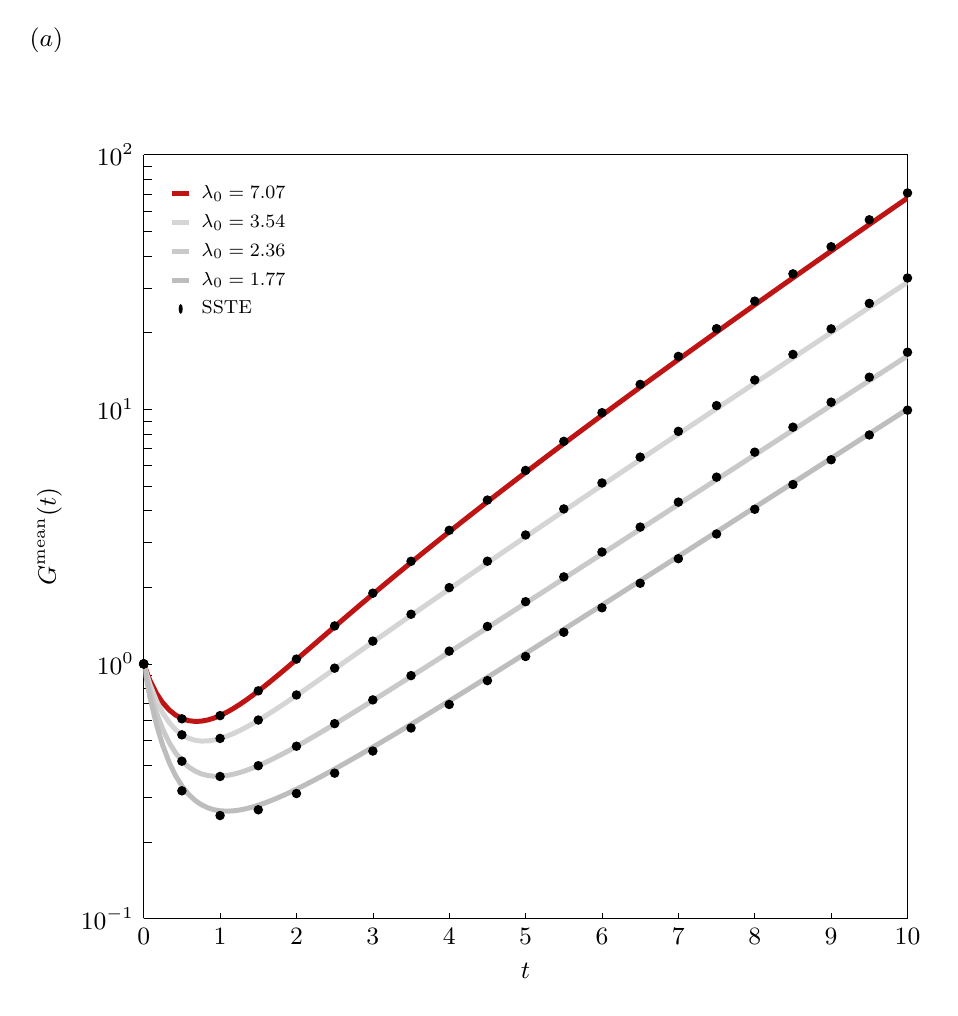
\begin{tikzpicture}

\begin{axis}[%
width=11.252in,
height=7.131in,
at={(1.887in,0.962in)},
scale only axis,
clip=true,
separate axis lines,
every outer x axis line/.append style={black},
every x tick label/.append style={font=\color{black}},
every x tick/.append style={black},
xmin=0,
xmax=10,
xlabel={$t$},
every outer y axis line/.append style={black},
every y tick label/.append style={font=\color{black}},
every y tick/.append style={black},
ymode=log,
ymin=0.1,
ymax=100,
yminorticks=true,
ylabel={$\mathscr{G}^{\mathrm{mean}}(t)$},
axis background/.style={fill=white},
legend style={at={(0.03,0.97)}, anchor=north west, legend cell align=left, align=left},
clip=true,
clip mode=individual,
axis lines=box,
xtick pos=bottom,
ytick pos=left,
tick align=inside,
major tick length=2pt,
width=0.8\linewidth,
height=0.8\linewidth,
every axis/.append style={font=\fontsize{9}{9}\selectfont},xlabel style={font=\fontsize{9}{9}\selectfont},title style={font=\fontsize{9}{9}\selectfont},
legend style={font=\fontsize{8}{9}\selectfont,inner sep=1pt,row sep=1pt,column sep=2pt,nodes={scale=0.85},draw=none},legend image post style={xscale=0.35},
legend columns=1,
scaled x ticks=false,
tick label style={/pgf/number format/fixed,/pgf/number format/precision=2},
every x tick label/.append style={font=\fontsize{9}{9}\selectfont\color{black}},
every y tick label/.append style={font=\fontsize{9}{9}\selectfont\color{black}},
,,
colormap={sigmamap}{rgb(0.0000)=(0.0200,0.1880,0.3800); rgb(0.1000)=(0.0743,0.3456,0.5616); rgb(0.2000)=(0.1918,0.4980,0.7060); rgb(0.3000)=(0.3890,0.6708,0.8226); rgb(0.4000)=(0.7552,0.8682,0.9228); rgb(0.5000)=(0.9690,0.9689,0.9689); rgb(0.6000)=(0.9425,0.8044,0.7614); rgb(0.7000)=(0.8767,0.4910,0.4020); rgb(0.8000)=(0.7869,0.2866,0.2470); rgb(0.9000)=(0.6186,0.1239,0.1568); rgb(1.0000)=(0.4040,0.0000,0.1220)}
]
\addplot [color=mycolor1, line width=1.8pt]
  table[row sep=crcr]{%
0	1\\
0.08	0.863137158521505\\
0.168	0.765296195121739\\
0.248	0.70474397683936\\
0.336	0.658588067607769\\
0.416	0.629965624874714\\
0.504	0.609519584109834\\
0.584	0.598892908179321\\
0.672	0.594352800620287\\
0.752000000000001	0.595723893901938\\
0.840000000000001	0.602453019766551\\
0.920000000000001	0.612775592295249\\
1	0.626711973705201\\
1.088	0.645872140261718\\
1.168	0.666532028500899\\
1.256	0.692615375910713\\
1.336	0.719241218543471\\
1.424	0.75161809759949\\
1.504	0.783785847991089\\
1.592	0.822122085993051\\
1.672	0.859627742041189\\
1.752	0.899650303696986\\
1.84	0.94658590309429\\
1.92	0.991917281242138\\
2.008	1.04474302259802\\
2.088	1.09549773591915\\
2.176	1.15438823944275\\
2.256	1.21076558561448\\
2.344	1.27598138132431\\
2.424	1.33825346035854\\
2.512	1.41013060368432\\
2.592	1.47863494697464\\
2.672	1.55024351361084\\
2.76	1.63271408325125\\
2.84	1.71116430192978\\
2.928	1.80141989337375\\
3.008	1.88719744834199\\
3.096	1.98580457936394\\
3.176	2.07945400275672\\
3.264	2.18704447946353\\
3.344	2.28917040355475\\
3.432	2.40644321391367\\
3.512	2.51771252197615\\
3.592	2.6335889910158\\
3.68	2.76658138177793\\
3.76	2.89270580804419\\
3.848	3.03742035263772\\
3.928	3.1746277528457\\
4.016	3.33202369135629\\
4.096	3.48122430690785\\
4.184	3.65234635855449\\
4.264	3.81453076764412\\
4.344	3.98327082575806\\
4.432	4.17675989630082\\
4.512	4.36010508177377\\
4.6	4.57031481138781\\
4.68	4.76948043259263\\
4.768	4.99780315637551\\
4.848	5.21410727490269\\
4.936	5.46205258737654\\
5.016	5.69692387401654\\
5.104	5.96612764098106\\
5.184	6.22111391381719\\
5.264	6.48625964894577\\
5.352	6.79012553863693\\
5.432	7.07790869573738\\
5.52	7.40769197688594\\
5.6	7.71999688768499\\
5.688	8.07785384695352\\
5.768	8.41671957503659\\
5.856	8.80498325633162\\
5.936	9.17261573798088\\
6.024	9.59380981525452\\
6.104	9.99259495760747\\
6.184	10.407109026888\\
6.272	10.8819664995123\\
6.352	11.3315143903061\\
6.44	11.8464706574774\\
6.52	12.3339470364914\\
6.608	12.8923125156637\\
6.68800000000001	13.4208459890154\\
6.77600000000001	14.0261982991293\\
6.85600000000001	14.5991696840653\\
6.93600000000001	15.1945683338136\\
7.02400000000001	15.876436477224\\
7.10400000000001	16.5217667285783\\
7.19200000000001	17.2607682106632\\
7.27200000000001	17.9601231757078\\
7.36000000000001	18.7609370534059\\
7.44000000000001	19.5187369929625\\
7.52800000000001	20.3864158406654\\
7.60800000000001	21.207433434276\\
7.69600000000001	22.1474321520764\\
7.77600000000001	23.0368196368196\\
7.85600000000001	23.9606924910561\\
7.94400000000001	25.0183446871354\\
8.024	26.018949051088\\
8.11199999999999	27.1643640821777\\
8.19199999999998	28.2479219793519\\
8.27999999999997	29.4882088762784\\
8.35999999999997	30.6614326209336\\
8.44799999999996	32.0042598205101\\
8.52799999999995	33.2743891696673\\
8.61599999999994	34.7280268165682\\
8.69599999999993	36.1028687705243\\
8.77599999999992	37.5304930532827\\
8.86399999999991	39.1642054407962\\
8.9439999999999	40.7091946766412\\
9.03199999999989	42.4770841710685\\
9.11199999999988	44.1488397483288\\
9.19999999999987	46.0616415823677\\
9.27999999999986	47.870293520584\\
9.36799999999985	49.9395735308096\\
9.44799999999985	51.8960342800602\\
9.52799999999984	53.9269569894389\\
9.61599999999983	56.2502719535687\\
9.69599999999982	58.4466649750828\\
9.78399999999981	60.9590746898465\\
9.8639999999998	63.3340433754666\\
9.95199999999979	66.0505038538592\\
10.0319999999998	68.6181527059567\\
10.1199999999998	71.5547578800136\\
10.1999999999998	74.3302622980936\\
10.2879999999998	77.504325438466\\
10.3679999999997	80.5040080619984\\
10.4479999999997	83.6165323444928\\
10.5359999999997	87.17556024128\\
10.6159999999997	90.5386279632922\\
10.7039999999997	94.3838016223578\\
10.7839999999997	98.0169362234784\\
10.8719999999997	102.17051665725\\
10.9519999999997	106.09469307459\\
11.0399999999997	110.580591951725\\
11.1199999999997	114.818336213295\\
11.2079999999997	119.66222855866\\
11.2879999999996	124.237723147983\\
11.3679999999996	128.983059192458\\
11.4559999999996	134.406361683826\\
11.5359999999996	139.528410766155\\
11.6239999999996	145.381653212772\\
11.7039999999996	150.909191711203\\
11.7919999999996	157.225149158398\\
11.8719999999996	163.189023685422\\
11.9599999999996	170.002820882748\\
12.0399999999996	176.436081620031\\
12.1199999999996	183.105150249691\\
12.2079999999995	190.723383948328\\
12.2879999999995	197.914952576998\\
12.3759999999995	206.129096813346\\
12.4559999999995	213.882288496777\\
12.5439999999995	222.736852337883\\
12.6239999999995	231.093508923673\\
12.7119999999995	240.636080951151\\
12.7919999999995	249.640926243071\\
12.8799999999995	259.922357664499\\
12.9599999999995	269.623167158641\\
13.0399999999995	279.673109577726\\
13.1279999999994	291.14553911633\\
13.2079999999994	301.967923572421\\
13.2959999999994	314.320409887543\\
13.3759999999994	325.971339675488\\
13.4639999999994	339.267599744497\\
13.5439999999994	351.806868281739\\
13.6319999999994	366.114785496255\\
13.7119999999994	379.60607263263\\
13.7919999999994	393.574261837076\\
13.8799999999994	409.508988640465\\
13.9599999999993	424.530730198167\\
14.0479999999993	441.664553958808\\
14.1279999999993	457.814025783034\\
14.2159999999993	476.231044880986\\
14.2959999999993	493.587027276652\\
14.3839999999993	513.376519419052\\
14.4639999999993	532.02260770615\\
14.5519999999993	553.279264672947\\
14.6319999999993	573.304083115019\\
14.7119999999993	594.018101769329\\
14.7999999999993	617.62566226783\\
14.8799999999992	639.858881816661\\
14.9679999999992	665.192894843786\\
15.0479999999992	689.047311133611\\
15.1359999999992	716.223115297006\\
15.2159999999992	741.806489943681\\
15.3039999999992	770.94587927322\\
15.3839999999992	798.371943886715\\
15.4719999999992	829.603389177732\\
15.5519999999992	858.992043137176\\
15.6319999999992	889.359242283781\\
15.7199999999992	923.928405098054\\
15.7999999999991	956.446859195702\\
15.8879999999991	993.456276516502\\
15.9679999999991	1028.26195046884\\
16.0559999999991	1067.86489056044\\
16.1359999999991	1105.10052651647\\
16.2239999999991	1147.45779408721\\
16.3039999999991	1187.27305534548\\
16.3839999999991	1228.37135237476\\
16.4719999999991	1275.10473645266\\
16.5519999999991	1319.01650020257\\
16.6399999999991	1368.93573177344\\
16.719999999999	1415.82825788342\\
16.807999999999	1469.12134783689\\
16.887999999999	1519.16919198034\\
16.975999999999	1576.032162967\\
17.055999999999	1629.41718024179\\
17.143999999999	1690.05409305365\\
17.223999999999	1746.9654457506\\
17.303999999999	1805.62460539367\\
17.391999999999	1872.22251949208\\
17.471999999999	1934.70054200388\\
17.559999999999	2005.61212405685\\
17.6399999999989	2072.11606621728\\
17.7279999999989	2147.57297085521\\
17.8079999999989	2218.31692861305\\
17.8959999999989	2298.55846287473\\
17.9759999999989	2373.76339420429\\
18.0639999999989	2459.03629466115\\
18.1439999999989	2538.92979045099\\
18.2239999999989	2621.13778212532\\
18.3119999999989	2714.30393956954\\
18.3919999999989	2801.54796650997\\
18.4799999999989	2900.38646595288\\
18.5599999999988	2992.90918580977\\
18.6479999999988	3097.68996918807\\
18.7279999999988	3195.73940996572\\
18.8159999999988	3306.73805286356\\
18.8959999999988	3410.56709685279\\
18.9759999999988	3517.23847523236\\
19.0639999999988	3637.9299897827\\
19.1439999999988	3750.76186920952\\
19.2319999999988	3878.3737456284\\
19.3119999999988	3997.62830110731\\
19.3999999999988	4132.45038329951\\
19.4799999999987	4258.39221937926\\
19.5679999999987	4400.71654244535\\
19.6479999999987	4533.61179447231\\
19.7359999999987	4683.73154260114\\
19.8159999999987	4823.84687966257\\
19.8959999999987	4967.49396010987\\
19.9839999999987	5129.65675901201\\
20.0639999999987	5280.91619927742\\
20.1519999999987	5451.59767458955\\
20.2319999999987	5610.73250814424\\
20.3199999999987	5790.22012642598\\
20.3999999999986	5957.48963623982\\
20.4879999999986	6146.06594037093\\
20.5679999999986	6321.72418019434\\
20.6559999999986	6519.66510112123\\
20.7359999999986	6703.95930470078\\
20.8159999999986	6892.45036347861\\
20.9039999999986	7104.70122936248\\
20.9839999999986	7302.17711952195\\
21.0719999999986	7524.43548575096\\
21.1519999999986	7731.11899942858\\
21.2399999999985	7963.62295259907\\
21.3199999999985	8179.72368748792\\
21.4079999999985	8422.69568105594\\
21.4879999999985	8648.40798319373\\
21.5679999999985	8878.76056699721\\
21.6559999999985	9137.55334768161\\
21.7359999999985	9377.77195965913\\
21.8239999999985	9647.50128907282\\
21.9039999999985	9897.73313659324\\
21.9919999999985	10178.5486148553\\
22.0719999999985	10438.9179203066\\
22.1599999999984	10730.9425847312\\
22.2399999999984	11001.5482536085\\
22.3279999999984	11304.876003637\\
22.4079999999984	11585.7892803033\\
22.4879999999984	11871.6273688968\\
22.5759999999984	12191.7444388079\\
22.6559999999984	12487.9398226717\\
22.7439999999984	12819.4506258254\\
22.8239999999984	13125.9961152975\\
22.9119999999984	13468.8734906897\\
22.9919999999984	13785.7263701486\\
23.0799999999983	14139.902931539\\
23.1599999999983	14466.9829120455\\
23.2479999999983	14832.3488873319\\
23.3279999999983	15169.536238794\\
23.4079999999983	15511.4826799179\\
23.4959999999983	15893.0714475953\\
23.5759999999983	16244.873025402\\
23.6639999999983	16637.1852018458\\
23.7439999999983	16998.6180422679\\
23.8319999999983	17401.3833149078\\
23.9119999999983	17772.1796362877\\
23.9999999999982	18185.0790511946\\
24.0799999999982	18564.92664146\\
24.1599999999982	18948.9616998966\\
24.2479999999982	19376.134378848\\
24.3279999999982	19768.6785234199\\
24.4159999999982	20204.9851312068\\
24.4959999999982	20605.616638405\\
24.5839999999982	21050.5695218467\\
24.6639999999982	21458.823763223\\
24.7519999999982	21911.8887809043\\
24.8319999999982	22327.2596114919\\
24.9199999999981	22787.8578890932\\
24.9999999999981	23209.7994473818\\
};
\addlegendentry{$\lambda_0=7.07$}

\addplot [color=mycolor2, line width=1.8pt]
  table[row sep=crcr]{%
0	1\\
0.08	0.832819704066107\\
0.168	0.714683253153248\\
0.248	0.64222558102442\\
0.336	0.587026730695588\\
0.416	0.552268248773759\\
0.504	0.526239770653693\\
0.584	0.510957051120003\\
0.672	0.501266897007025\\
0.752000000000001	0.497634260728043\\
0.840000000000001	0.498268853598173\\
0.920000000000001	0.502365080522346\\
1	0.509317320266773\\
1.088	0.519829321027364\\
1.168	0.531685881906803\\
1.256	0.546992780402698\\
1.336	0.562786767973008\\
1.424	0.582069226497625\\
1.504	0.601228389733645\\
1.592	0.624005492144949\\
1.672	0.646200559436219\\
1.752	0.669773530817573\\
1.84	0.697265048201602\\
1.92	0.723660903198896\\
2.008	0.754233967753364\\
2.088	0.783428720554656\\
2.176	0.817096398143766\\
2.256	0.849133119079866\\
2.344	0.885972878230917\\
2.424	0.920946386854043\\
2.512	0.961086678958327\\
2.592	0.999133822099627\\
2.672	1.03870327442045\\
2.76	1.08403907359157\\
2.84	1.12694859775924\\
2.928	1.17607504326586\\
3.008	1.22254394253983\\
3.096	1.27571855160338\\
3.176	1.32599548507158\\
3.264	1.38350763017961\\
3.344	1.4378700240055\\
3.432	1.50004071072415\\
3.512	1.55879489320505\\
3.592	1.61975661699255\\
3.68	1.68945912810072\\
3.76	1.75531924536129\\
3.848	1.8306156273392\\
3.928	1.90175594582726\\
4.016	1.98308413940995\\
4.096	2.05991956005876\\
4.184	2.14775496336989\\
4.264	2.23073547206347\\
4.344	2.31681111790574\\
4.432	2.41520624420687\\
4.512	2.50816027146618\\
4.6	2.61441684500497\\
4.68	2.71479653181068\\
4.768	2.82954045681336\\
4.848	2.93793729752015\\
4.936	3.06184486519279\\
5.016	3.17889782063192\\
5.104	3.31269944234446\\
5.184	3.43909847985704\\
5.264	3.57020629587451\\
5.352	3.72007268133342\\
5.432	3.86164654232403\\
5.52	4.02347541800629\\
5.6	4.17634880784447\\
5.688	4.35109252457545\\
5.768	4.51616469792011\\
5.856	4.70485067029701\\
5.936	4.88309168395083\\
6.024	5.08682813697658\\
6.104	5.27928427320722\\
6.184	5.47890083099329\\
6.272	5.70706604279049\\
6.352	5.92259403335802\\
6.44	6.16894259700932\\
6.52	6.40164314932235\\
6.608	6.66761551252459\\
6.68800000000001	6.91884828099154\\
6.77600000000001	7.20599734068389\\
6.85600000000001	7.4772280421583\\
6.93600000000001	7.75852952676515\\
7.02400000000001	8.08003625929708\\
7.10400000000001	8.38371051461798\\
7.19200000000001	8.73077992469615\\
7.27200000000001	9.0585914721146\\
7.36000000000001	9.43323849037609\\
7.44000000000001	9.78708878800768\\
7.52800000000001	10.1914845975571\\
7.60800000000001	10.5734224450824\\
7.69600000000001	11.0099063428524\\
7.77600000000001	11.4221390556265\\
7.85600000000001	11.8496226965924\\
7.94400000000001	12.338136595384\\
8.024	12.7994888607299\\
8.11199999999999	13.3266909544546\\
8.19199999999998	13.8245651887723\\
8.27999999999997	14.3934844311703\\
8.35999999999997	14.9307381188624\\
8.44799999999996	15.544636302913\\
8.52799999999995	16.1243463966578\\
8.61599999999994	16.7867356161208\\
8.69599999999993	17.4122149745842\\
8.77599999999992	18.0607264519982\\
8.86399999999991	18.8016913561581\\
8.9439999999999	19.5013313013094\\
9.03199999999989	20.3006845496707\\
9.11199999999988	21.0554285088383\\
9.19999999999987	21.9177068050186\\
9.27999999999986	22.7318331052257\\
9.36799999999985	23.6619183172831\\
9.44799999999985	24.5400304522582\\
9.52799999999984	25.4503303706021\\
9.61599999999983	26.4902256829824\\
9.69599999999982	27.471952531396\\
9.78399999999981	28.5933966072787\\
9.8639999999998	29.6520657613237\\
9.95199999999979	30.8613503027007\\
10.0319999999998	32.0028930444898\\
10.1199999999998	33.3067836212315\\
10.1999999999998	34.5375773981777\\
10.2879999999998	35.94334785353\\
10.3679999999997	37.2702486049331\\
10.4479999999997	38.6454717214855\\
10.5359999999997	40.216094478701\\
10.6159999999997	41.6984934484664\\
10.7039999999997	43.3914369334648\\
10.7839999999997	44.9892060444985\\
10.8719999999997	46.8138131333496\\
10.9519999999997	48.5357554331821\\
11.0399999999997	50.5020620132785\\
11.1199999999997	52.3576324831401\\
11.2079999999997	54.4764164688637\\
11.2879999999996	56.4757680051309\\
11.3679999999996	58.5473699201293\\
11.4559999999996	60.9126338752825\\
11.5359999999996	63.1443844395034\\
11.6239999999996	65.6923506033964\\
11.7039999999996	68.0963481299812\\
11.7919999999996	70.8408016715023\\
11.8719999999996	73.4300262183668\\
11.9599999999996	76.3857549725686\\
12.0399999999996	79.174128762386\\
12.1199999999996	82.0625182054445\\
12.2079999999995	85.3594431792668\\
12.2879999999995	88.4693923365339\\
12.3759999999995	92.0189746995615\\
12.4559999999995	95.3670226702141\\
12.5439999999995	99.1880950766263\\
12.6239999999995	102.791962620024\\
12.7119999999995	106.904699876317\\
12.7919999999995	110.7833674195\\
12.8799999999995	115.209374662207\\
12.9599999999995	119.383164650541\\
13.0399999999995	123.705043043727\\
13.1279999999994	128.636234107579\\
13.2079999999994	133.285872554186\\
13.2959999999994	138.590597272469\\
13.3759999999994	143.592024813775\\
13.4639999999994	149.29761665036\\
13.5439999999994	154.676526269617\\
13.6319999999994	160.812205186686\\
13.7119999999994	166.596057129652\\
13.7919999999994	172.582930166104\\
13.8799999999994	179.411175985334\\
13.9599999999993	185.846988391208\\
14.0479999999993	193.186554890728\\
14.1279999999993	200.103619506876\\
14.2159999999993	207.991224962986\\
14.2959999999993	215.42401975176\\
14.3839999999993	223.898832507869\\
14.4639999999993	231.884126200704\\
14.5519999999993	240.987905604438\\
14.6319999999993	249.564888284411\\
14.7119999999993	258.438138380534\\
14.7999999999993	268.55254952509\\
14.8799999999992	278.080054027215\\
14.9679999999992	288.938939211143\\
15.0479999999992	299.166476641893\\
15.1359999999992	310.821773632205\\
15.2159999999992	321.798034377384\\
15.3039999999992	334.304966384045\\
15.3839999999992	346.081703471949\\
15.4719999999992	359.49894713095\\
15.5519999999992	372.131130785839\\
15.6319999999992	385.190963610323\\
15.7199999999992	400.066963646752\\
15.7999999999991	414.069604704096\\
15.8879999999991	430.017186045795\\
15.9679999999991	445.026257624301\\
16.0559999999991	462.117460068169\\
16.1359999999991	478.200361895172\\
16.2239999999991	496.511471275604\\
16.3039999999991	513.739545957733\\
16.3839999999991	531.539201830076\\
16.4719999999991	551.799975664408\\
16.5519999999991	570.857677572132\\
16.6399999999991	592.546702768952\\
16.719999999999	612.944270612799\\
16.807999999999	636.154011476638\\
16.887999999999	657.977782269284\\
16.975999999999	682.805760913825\\
17.055999999999	706.146749751861\\
17.143999999999	732.695721163306\\
17.223999999999	757.649778244723\\
17.303999999999	783.407093022594\\
17.391999999999	812.695862676171\\
17.471999999999	840.216895538401\\
17.559999999999	871.504696271981\\
17.6399999999989	900.897908690188\\
17.7279999999989	934.306962753992\\
17.8079999999989	965.686146880608\\
17.8959999999989	1001.34460881\\
17.9759999999989	1034.82900925262\\
18.0639999999989	1072.87109322147\\
18.1439999999989	1108.58551636145\\
18.2239999999989	1145.40735911637\\
18.3119999999989	1187.22651772528\\
18.3919999999989	1226.47298320323\\
18.4799999999989	1271.0348660341\\
18.5599999999988	1312.84490592299\\
18.6479999999988	1360.30555354604\\
18.7279999999988	1404.82393606636\\
18.8159999999988	1455.34580594717\\
18.8959999999988	1502.72314416194\\
18.9759999999988	1551.51652370401\\
19.0639999999988	1606.86788436829\\
19.1439999999988	1658.75323700946\\
19.2319999999988	1717.59576102619\\
19.3119999999988	1772.73813143835\\
19.3999999999988	1835.25653424755\\
19.4799999999987	1893.82670321931\\
19.5679999999987	1960.21195865531\\
19.6479999999987	2022.38634103213\\
19.7359999999987	2092.83554912661\\
19.8159999999987	2158.79605475464\\
19.8959999999987	2226.6249628602\\
19.9839999999987	2303.44612166693\\
20.0639999999987	2375.3393392842\\
20.1519999999987	2456.73764333926\\
20.2319999999987	2532.88982302757\\
20.3199999999987	2619.0820061984\\
20.3999999999986	2699.69247871382\\
20.4879999999986	2790.90023855902\\
20.5679999999986	2876.17266815102\\
20.6559999999986	2972.6222567314\\
20.7359999999986	3062.76424098217\\
20.8159999999986	3155.29905285585\\
20.9039999999986	3259.90860328515\\
20.9839999999986	3357.62562395908\\
21.0719999999986	3468.05365652886\\
21.1519999999986	3571.16811317298\\
21.2399999999985	3687.65259934521\\
21.3199999999985	3796.38177877745\\
21.4079999999985	3919.16258473917\\
21.4879999999985	4033.72514112161\\
21.5679999999985	4151.14255264835\\
21.6559999999985	4283.65841360933\\
21.7359999999985	4407.23283276937\\
21.8239999999985	4546.64177245601\\
21.9039999999985	4676.59177382029\\
21.9919999999985	4823.13345958748\\
22.0719999999985	4959.67598023849\\
22.1599999999984	5113.58771399828\\
22.2399999999984	5256.93700710458\\
22.3279999999984	5418.45252807397\\
22.4079999999984	5568.81903229563\\
22.4879999999984	5722.59961858051\\
22.5759999999984	5895.75635116913\\
22.6559999999984	6056.8552298482\\
22.7439999999984	6238.17069437374\\
22.8239999999984	6406.78345125953\\
22.9119999999984	6596.46837152687\\
22.9919999999984	6772.78219587675\\
23.0799999999983	6971.03724592516\\
23.1599999999983	7155.2294326121\\
23.2479999999983	7362.2435481526\\
23.3279999999983	7554.47992673137\\
23.4079999999983	7750.60142019731\\
23.4959999999983	7970.86183631874\\
23.5759999999983	8175.24787935207\\
23.6639999999983	8404.67318025266\\
23.7439999999983	8617.4540406147\\
23.8319999999983	8856.17819664035\\
23.9119999999983	9077.46674987961\\
23.9999999999982	9325.60361414408\\
24.0799999999982	9555.49354482151\\
24.1599999999982	9789.50627172294\\
24.2479999999982	10051.6988461908\\
24.3279999999982	10294.4123213728\\
24.4159999999982	10566.2001332452\\
24.4959999999982	10817.6526950032\\
24.5839999999982	11099.0641393223\\
24.6639999999982	11359.2686401108\\
24.7519999999982	11650.3031085644\\
24.8319999999982	11919.2451672592\\
24.9199999999981	12219.8711603627\\
24.9999999999981	12497.5074839751\\
};
\addlegendentry{$\lambda_0=3.54$}

\addplot [color=mycolor3, line width=1.8pt]
  table[row sep=crcr]{%
0	1\\
0.08	0.787130537175682\\
0.168	0.641812316602565\\
0.248	0.554861742170152\\
0.336	0.48930183522127\\
0.416	0.447683888717454\\
0.504	0.415395635661876\\
0.584	0.394846070670004\\
0.672	0.379349754121433\\
0.752000000000001	0.370187242086496\\
0.840000000000001	0.3643070861304\\
0.920000000000001	0.362011817534288\\
1	0.362085889871243\\
1.088	0.364446050548875\\
1.168	0.368348884565332\\
1.256	0.374304587826573\\
1.336	0.381048679812777\\
1.424	0.389771796648539\\
1.504	0.398780956387305\\
1.592	0.409784859888156\\
1.672	0.420720356101917\\
1.752	0.432498409841689\\
1.84	0.446389190288313\\
1.92	0.459842273724704\\
2.008	0.47552959569955\\
2.088	0.4905894389037\\
2.176	0.508029665397057\\
2.256	0.524680709516023\\
2.344	0.543879246027102\\
2.424	0.562144098958161\\
2.512	0.583142778536841\\
2.592	0.603073146682235\\
2.672	0.623821731052117\\
2.76	0.647613294866366\\
2.84	0.670145373196348\\
2.928	0.695953324811225\\
3.008	0.720372399405414\\
3.096	0.748320070637292\\
3.176	0.774746570521144\\
3.264	0.804975322031563\\
3.344	0.833545689476253\\
3.432	0.866214235989974\\
3.512	0.897080568287754\\
3.592	0.929098220596062\\
3.68	0.965694922365792\\
3.76	1.00026185913691\\
3.848	1.03976596355549\\
3.928	1.07707389590871\\
4.016	1.11970554217061\\
4.096	1.15996321067151\\
4.184	1.20596173994776\\
4.264	1.24939581223081\\
4.344	1.29442759105286\\
4.432	1.345876988159\\
4.512	1.39445483927423\\
4.6	1.44995378926163\\
4.68	1.50235369279386\\
4.768	1.56221783157325\\
4.848	1.61873806414432\\
4.936	1.68330840885843\\
5.016	1.74427113479602\\
5.104	1.81391591619913\\
5.184	1.87966892883598\\
5.264	1.94783317961545\\
5.352	2.02570420894914\\
5.432	2.09922305301262\\
5.52	2.18321070776634\\
5.6	2.2625039057872\\
5.688	2.35308771125838\\
5.768	2.4386079577897\\
5.856	2.53630501403917\\
5.936	2.62854043439975\\
6.024	2.73390826935368\\
6.104	2.83338511326685\\
6.184	2.93650700345734\\
6.272	3.05431030436585\\
6.352	3.16552634660867\\
6.44	3.29257529284389\\
6.52	3.41251911511942\\
6.608	3.54953727681315\\
6.68800000000001	3.67889172308447\\
6.77600000000001	3.82665883497539\\
6.85600000000001	3.96615971825062\\
6.93600000000001	4.11076723387684\\
7.02400000000001	4.27595610153293\\
7.10400000000001	4.43190169054578\\
7.19200000000001	4.61004027513143\\
7.27200000000001	4.77820893937936\\
7.36000000000001	4.97030766447877\\
7.44000000000001	5.15165276827184\\
7.52800000000001	5.35880006256407\\
7.60800000000001	5.55434852739859\\
7.69600000000001	5.77771674867596\\
7.77600000000001	5.98857463608754\\
7.85600000000001	6.20713593631519\\
7.94400000000001	6.4567849477594\\
8.024	6.69244588535137\\
8.11199999999999	6.96162203453913\\
8.19199999999998	7.21571140745643\\
8.27999999999997	7.50593145740044\\
8.35999999999997	7.77988004407015\\
8.44799999999996	8.09277709221404\\
8.52799999999995	8.38812534238097\\
8.61599999999994	8.72545758684236\\
8.69599999999993	9.04386387887826\\
8.77599999999992	9.37386949719721\\
8.86399999999991	9.75077353418169\\
8.9439999999999	10.106519744675\\
9.03199999999989	10.5128131073139\\
9.11199999999988	10.8962898368524\\
9.19999999999987	11.3342433633575\\
9.27999999999986	11.7475921707616\\
9.36799999999985	12.2196496145268\\
9.44799999999985	12.6651750130385\\
9.52799999999984	13.1268828866729\\
9.61599999999983	13.6541475410798\\
9.69599999999982	14.1517576672186\\
9.78399999999981	14.7200066935816\\
9.8639999999998	15.2562812235038\\
9.95199999999979	15.8686659541854\\
10.0319999999998	16.4465761043058\\
10.1199999999998	17.1064861995222\\
10.1999999999998	17.7292277065898\\
10.2879999999998	18.4403087508468\\
10.3679999999997	19.1113184277698\\
10.4479999999997	19.8065952725136\\
10.5359999999997	20.6004642421724\\
10.6159999999997	21.3495611141851\\
10.7039999999997	22.2048538618727\\
10.7839999999997	23.0118835005741\\
10.8719999999997	23.9332906510792\\
10.9519999999997	24.8026740627602\\
11.0399999999997	25.7952374725451\\
11.1199999999997	26.7317263705127\\
11.2079999999997	27.8008646540396\\
11.2879999999996	28.8095654534244\\
11.3679999999996	29.8545569656299\\
11.4559999999996	31.0475007376103\\
11.5359999999996	32.1729452229135\\
11.6239999999996	33.4576826105528\\
11.7039999999996	34.6696789182956\\
11.7919999999996	36.0531628368136\\
11.8719999999996	37.358261453675\\
11.9599999999996	38.8479590575211\\
12.0399999999996	40.2531943270266\\
12.1199999999996	41.7087350802563\\
12.2079999999995	43.3700481074514\\
12.2879999999995	44.9370672258285\\
12.3759999999995	46.7255381140911\\
12.4559999999995	48.4124208241357\\
12.5439999999995	50.3376050662995\\
12.6239999999995	52.153349976566\\
12.7119999999995	54.22550098167\\
12.7919999999995	56.1797629134904\\
12.8799999999995	58.409880607148\\
12.9599999999995	60.5130161627528\\
13.0399999999995	62.6908997217316\\
13.1279999999994	65.1760146864655\\
13.2079999999994	67.5194461662676\\
13.2959999999994	70.1933182891266\\
13.3759999999994	72.7146069888535\\
13.4639999999994	75.5912546052707\\
13.5439999999994	78.3035933473953\\
13.6319999999994	81.3980389785611\\
13.7119999999994	84.3155637073944\\
13.7919999999994	87.3360538916131\\
13.8799999999994	90.7817544677395\\
13.9599999999993	94.0301563374406\\
14.0479999999993	97.7356182540901\\
14.1279999999993	101.228682699574\\
14.2159999999993	105.212970188832\\
14.2959999999993	108.968626899406\\
14.3839999999993	113.252142439851\\
14.4639999999993	117.289576493515\\
14.5519999999993	121.894147340322\\
14.6319999999993	126.233879973747\\
14.7119999999993	130.725185951388\\
14.7999999999993	135.846823043272\\
14.8799999999992	140.673344189884\\
14.9679999999992	146.176814118928\\
15.0479999999992	151.362755806784\\
15.1359999999992	157.275579285267\\
15.2159999999992	162.846798041752\\
15.3039999999992	169.198366895376\\
15.3839999999992	175.182471270219\\
15.4719999999992	182.004161977523\\
15.5519999999992	188.430618123296\\
15.6319999999992	195.078641145107\\
15.7199999999992	202.656152568749\\
15.7999999999991	209.793654950021\\
15.8879999999991	217.928298994414\\
15.9679999999991	225.58983160784\\
16.0559999999991	234.320841275233\\
16.1359999999991	242.543216594743\\
16.2239999999991	251.912381736901\\
16.3039999999991	260.734800587749\\
16.3839999999991	269.85745838112\\
16.4719999999991	280.250792714061\\
16.5519999999991	290.036006212154\\
16.6399999999991	301.182903132889\\
16.719999999999	311.676361554343\\
16.807999999999	323.628634557474\\
16.887999999999	334.878890412734\\
16.975999999999	347.691582216295\\
17.055999999999	359.750196937428\\
17.143999999999	373.481741633763\\
17.223999999999	386.403434673111\\
17.303999999999	399.75630429805\\
17.391999999999	414.958624475379\\
17.471999999999	429.261443467586\\
17.559999999999	445.542978137445\\
17.6399999999989	460.858946046622\\
17.7279999999989	478.291226617529\\
17.8079999999989	494.6872399298\\
17.8959999999989	513.345951594153\\
17.9759999999989	530.892762372718\\
18.0639999999989	550.85791890401\\
18.1439999999989	569.63029376586\\
18.2239999999989	589.013753716761\\
18.3119999999989	611.063290822764\\
18.3919999999989	631.790357151732\\
18.4799999999989	655.364217271166\\
18.5599999999988	677.520276126239\\
18.6479999999988	702.714869933341\\
18.7279999999988	726.389864484235\\
18.8159999999988	753.306697871869\\
18.8959999999988	778.595277118178\\
18.9759999999988	804.686898180512\\
19.0639999999988	834.342774170131\\
19.1439999999988	862.196602423997\\
19.2319999999988	893.849011597788\\
19.3119999999988	923.571950566369\\
19.3999999999988	957.341315002275\\
19.4799999999987	989.045439543296\\
19.5679999999987	1025.05793337862\\
19.6479999999987	1058.86060243213\\
19.7359999999987	1097.24826920973\\
19.8159999999987	1133.27222595233\\
19.8959999999987	1170.39866377657\\
19.9839999999987	1212.54653857949\\
20.0639999999987	1252.08547426275\\
20.1519999999987	1296.96136508499\\
20.2319999999987	1339.0492073044\\
20.3199999999987	1386.80624306283\\
20.3999999999986	1431.58500678263\\
20.4879999999986	1482.38249675317\\
20.5679999999986	1529.99982194529\\
20.6559999999986	1584.00326321939\\
20.7359999999986	1634.61240908427\\
20.8159999999986	1686.70172072841\\
20.9039999999986	1745.7532778068\\
20.9839999999986	1801.07084298198\\
21.0719999999986	1863.76457633388\\
21.1519999999986	1922.47736347849\\
21.2399999999985	1988.99991001223\\
21.3199999999985	2051.28025865526\\
21.4079999999985	2121.82408698602\\
21.4879999999985	2187.84955922264\\
21.5679999999985	2255.72230078778\\
21.6559999999985	2332.56597676339\\
21.7359999999985	2404.45509256605\\
21.8239999999985	2485.82044154641\\
21.9039999999985	2561.91552246627\\
21.9919999999985	2648.01354478012\\
22.0719999999985	2728.50855664564\\
22.1599999999984	2819.55487838109\\
22.2399999999984	2904.64780951612\\
22.3279999999984	3000.86226522773\\
22.4079999999984	3090.75471935957\\
22.4879999999984	3183.00445227271\\
22.5759999999984	3287.25760397398\\
22.6559999999984	3384.61007277223\\
22.7439999999984	3494.59058932196\\
22.8239999999984	3597.2542176917\\
22.9119999999984	3713.1924042996\\
22.9919999999984	3821.37734367479\\
23.0799999999983	3943.50503500289\\
23.1599999999983	4057.42247252942\\
23.2479999999983	4185.97223225781\\
23.3279999999983	4305.83362684303\\
23.4079999999983	4428.59966895139\\
23.4959999999983	4567.05411069683\\
23.5759999999983	4696.07496554323\\
23.6639999999983	4841.52463090505\\
23.7439999999983	4977.00865993169\\
23.8319999999983	5129.68125520841\\
23.9119999999983	5271.83384520376\\
23.9999999999982	5431.95320507326\\
24.0799999999982	5580.97565867119\\
24.1599999999982	5733.33874610732\\
24.2479999999982	5904.84882936568\\
24.3279999999982	6064.36894026343\\
24.4159999999982	6243.8550611007\\
24.4959999999982	6410.71810512614\\
24.5839999999982	6598.38025486152\\
24.6639999999982	6772.76359511876\\
24.7519999999982	6968.79157658831\\
24.8319999999982	7150.86258137793\\
24.9199999999981	7355.43437895018\\
24.9999999999981	7545.3489078087\\
};
\addlegendentry{$\lambda_0=2.36$}

\addplot [color=mycolor4, line width=1.8pt]
  table[row sep=crcr]{%
0	1\\
0.08	0.743470359435956\\
0.168	0.576117066798391\\
0.248	0.479642934855529\\
0.336	0.408811762327586\\
0.416	0.364561344340258\\
0.504	0.330338524359988\\
0.584	0.308289419628975\\
0.672	0.291081445996212\\
0.752000000000001	0.280158121223481\\
0.840000000000001	0.272038866716628\\
0.920000000000001	0.267407177271807\\
1	0.26485295974835\\
1.088	0.263989893371575\\
1.168	0.264669293847231\\
1.256	0.266767822810731\\
1.336	0.269731638154394\\
1.424	0.274004455791523\\
1.504	0.27870886531608\\
1.592	0.284697975259161\\
1.672	0.29082346419647\\
1.752	0.297553805893507\\
1.84	0.305617622430504\\
1.92	0.313522703969406\\
2.008	0.32282861008677\\
2.088	0.331830332571826\\
2.176	0.342318934754722\\
2.256	0.352383296698101\\
2.344	0.364035550954585\\
2.424	0.375159422835842\\
2.512	0.387985247574226\\
2.592	0.400188232505783\\
2.672	0.412917225311241\\
2.76	0.427538766866174\\
2.84	0.441407057066274\\
2.928	0.457311916896953\\
3.008	0.472377265762158\\
3.096	0.489635607373427\\
3.176	0.50596752405943\\
3.264	0.524661846079814\\
3.344	0.542340652028643\\
3.432	0.562565030844738\\
3.512	0.581681379023047\\
3.592	0.601517084481202\\
3.68	0.624195851986129\\
3.76	0.645621536133612\\
3.848	0.670111691580458\\
3.928	0.693243416859662\\
4.016	0.71967846655509\\
4.096	0.74464301265043\\
4.184	0.773168501316628\\
4.264	0.800103849841504\\
4.344	0.828029571620335\\
4.432	0.859933898833739\\
4.512	0.890055888274284\\
4.6	0.924467007479446\\
4.68	0.956953804663458\\
4.768	0.994064546860266\\
4.848	1.02909843577446\\
4.936	1.06911726037746\\
5.016	1.10689521981277\\
5.104	1.15004731307429\\
5.184	1.19078206314599\\
5.264	1.23300442678649\\
5.352	1.28123168890008\\
5.432	1.32675607677033\\
5.52	1.37875419561348\\
5.6	1.42783744549213\\
5.688	1.4838998349743\\
5.768	1.53681894783516\\
5.856	1.59726201991524\\
5.936	1.65431567709954\\
6.024	1.71948057634835\\
6.104	1.78099077796708\\
6.184	1.84474352517692\\
6.272	1.91755908608255\\
6.352	1.98629010768177\\
6.44	2.06479105199856\\
6.52	2.13888799080671\\
6.608	2.22351696897157\\
6.68800000000001	2.30339754375227\\
6.77600000000001	2.39463152585653\\
6.85600000000001	2.48074582024385\\
6.93600000000001	2.56999675062489\\
7.02400000000001	2.67193163400676\\
7.10400000000001	2.76814510889968\\
7.19200000000001	2.87803101986843\\
7.27200000000001	2.98174826577602\\
7.36000000000001	3.1002031083347\\
7.44000000000001	3.21200711333618\\
7.52800000000001	3.33969644359591\\
7.60800000000001	3.46021513102405\\
7.69600000000001	3.59785577714718\\
7.77600000000001	3.72776541773987\\
7.85600000000001	3.862399575797\\
7.94400000000001	4.01615825141499\\
8.024	4.16127786641281\\
8.11199999999999	4.32700921436304\\
8.19199999999998	4.48342664675097\\
8.27999999999997	4.66205792544116\\
8.35999999999997	4.83064785685359\\
8.44799999999996	5.02317742296469\\
8.52799999999995	5.20488156652133\\
8.61599999999994	5.41238424541112\\
8.69599999999993	5.60821640577552\\
8.77599999999992	5.81115479306449\\
8.86399999999991	6.04290076860931\\
8.9439999999999	6.26160711127599\\
9.03199999999989	6.5113548455803\\
9.11199999999988	6.74704571033657\\
9.19999999999987	7.01618354461257\\
9.27999999999986	7.27016827369722\\
9.36799999999985	7.5601903634255\\
9.44799999999985	7.83387803446804\\
9.52799999999984	8.11747411585883\\
9.61599999999983	8.44129917769126\\
9.69599999999982	8.74687650817078\\
9.78399999999981	9.09579337029708\\
9.8639999999998	9.42504130990313\\
9.95199999999979	9.80097749820868\\
10.0319999999998	10.1557135453726\\
10.1199999999998	10.5607426952924\\
10.1999999999998	10.9429220282489\\
10.2879999999998	11.3792747543705\\
10.3679999999997	11.7910004640787\\
10.4479999999997	12.21758071469\\
10.5359999999997	12.7046100787846\\
10.6159999999997	13.1641350384626\\
10.7039999999997	13.6887638783407\\
10.7839999999997	14.1837518085127\\
10.8719999999997	14.7488526514364\\
10.9519999999997	15.2820113847139\\
11.0399999999997	15.8906728338604\\
11.1199999999997	16.4649137334066\\
11.2079999999997	17.1204563605971\\
11.2879999999996	17.7389092724918\\
11.3679999999996	18.3795829734243\\
11.4559999999996	19.1109319041717\\
11.5359999999996	19.8008713718888\\
11.6239999999996	20.5884343806924\\
11.7039999999996	21.3313817896044\\
11.7919999999996	22.1794261568199\\
11.8719999999996	22.9794028440583\\
11.9599999999996	23.8925138914551\\
12.0399999999996	24.7538406238273\\
12.1199999999996	25.6459925916612\\
12.2079999999995	26.6642634167039\\
12.2879999999995	27.6247372343141\\
12.3759999999995	28.7209495282391\\
12.4559999999995	29.7549038748687\\
12.5439999999995	30.9349383853387\\
12.6239999999995	32.0479133448295\\
12.7119999999995	33.3180851292841\\
12.7919999999995	34.5160294749689\\
12.8799999999995	35.8831189124136\\
12.9599999999995	37.1724192338377\\
13.0399999999995	38.5076019150473\\
13.1279999999994	40.03121690435\\
13.2079999999994	41.4680499007916\\
13.2959999999994	43.1075925372543\\
13.3759999999994	44.6536847209131\\
13.4639999999994	46.4178249300737\\
13.5439999999994	48.0813401754795\\
13.6319999999994	49.9793793896437\\
13.7119999999994	51.769075362175\\
13.7919999999994	53.6221180893584\\
13.8799999999994	55.7362599914587\\
13.9599999999993	57.7295847820809\\
14.0479999999993	60.0036651629875\\
14.1279999999993	62.1476833450337\\
14.2159999999993	64.5935598909517\\
14.2959999999993	66.8994317530473\\
14.3839999999993	69.5298136727664\\
14.4639999999993	72.0094995173743\\
14.5519999999993	74.8380054012298\\
14.6319999999993	77.5043197253441\\
14.7119999999993	80.2642709177594\\
14.7999999999993	83.4122078739708\\
14.8799999999992	86.3793878985061\\
14.9679999999992	89.7634878053493\\
15.0479999999992	92.953080862236\\
15.1359999999992	96.5906250515255\\
15.2159999999992	100.018884287189\\
15.3039999999992	103.928367894044\\
15.3839999999992	107.612685371142\\
15.4719999999992	111.813896438205\\
15.5519999999992	115.772877025389\\
15.6319999999992	119.869560078944\\
15.7199999999992	124.540519310351\\
15.7999999999991	128.941712526306\\
15.8879999999991	133.959509586061\\
15.9679999999991	138.687165322899\\
16.0559999999991	144.076761633285\\
16.1359999999991	149.154334258738\\
16.2239999999991	154.942393978955\\
16.3039999999991	160.394932844985\\
16.3839999999991	166.035318436063\\
16.4719999999991	172.464174595208\\
16.5519999999991	178.519626824057\\
16.6399999999991	185.420984961522\\
16.719999999999	191.920932161725\\
16.807999999999	199.328223040718\\
16.887999999999	206.304047486509\\
16.975999999999	214.252913117244\\
17.055999999999	221.738064745098\\
17.143999999999	230.266486054508\\
17.223999999999	238.296600860448\\
17.303999999999	246.599412148355\\
17.391999999999	256.058053546416\\
17.471999999999	264.962690597738\\
17.559999999999	275.105866710262\\
17.6399999999989	284.653917683064\\
17.7279999999989	295.528805199244\\
17.8079999999989	305.764491227266\\
17.8959999999989	317.421238554331\\
17.9759999999989	328.391551910194\\
18.0639999999989	340.883433331412\\
18.1439999999989	352.638279482831\\
18.2239999999989	364.785134915351\\
18.3119999999989	378.6141966917\\
18.3919999999989	391.624888502212\\
18.4799999999989	406.435480177239\\
18.5599999999988	420.367761002939\\
18.6479999999988	436.225277472635\\
18.7279999999988	451.140332356766\\
18.8159999999988	468.11402908221\\
18.8959999999988	484.076630294433\\
18.9759999999988	500.561908890158\\
19.0639999999988	519.318457713057\\
19.1439999999988	536.953786114335\\
19.2319999999988	557.015721903897\\
19.3119999999988	575.8754286365\\
19.3999999999988	597.326764022613\\
19.4799999999987	617.489309159909\\
19.5679999999987	640.418687000969\\
19.6479999999987	661.966817192021\\
19.7359999999987	686.467679899568\\
19.8159999999987	709.488580939494\\
19.8959999999987	733.242770465368\\
19.9839999999987	760.244782309724\\
20.0639999999987	785.608873132757\\
20.1519999999987	814.435462490905\\
20.2319999999987	841.508263258122\\
20.3199999999987	872.270815357369\\
20.3999999999986	901.156068174385\\
20.4879999999986	933.971465715675\\
20.5679999999986	964.777972391395\\
20.6559999999986	999.768729170313\\
20.7359999999986	1032.61046750711\\
20.8159999999986	1066.46295230327\\
20.9039999999986	1104.90107854125\\
20.9839999999986	1140.96672608162\\
21.0719999999986	1181.90856286604\\
21.1519999999986	1220.31458871326\\
21.2399999999985	1263.90307765876\\
21.3199999999985	1304.78217449312\\
21.4079999999985	1351.16631154944\\
21.4879999999985	1394.65669795485\\
21.5679999999985	1439.44074653325\\
21.6559999999985	1490.23702422021\\
21.7359999999985	1537.84655204133\\
21.8239999999985	1591.83369174166\\
21.9039999999985	1642.42067055613\\
21.9919999999985	1699.76888223454\\
22.0719999999985	1753.49080094752\\
22.1599999999984	1814.37633234822\\
22.2399999999984	1871.39613283831\\
22.3279999999984	1936.0011813837\\
22.4079999999984	1996.48716179906\\
22.4879999999984	2058.68437806004\\
22.5759999999984	2129.12543176339\\
22.6559999999984	2195.04676811549\\
22.7439999999984	2269.68319841707\\
22.8239999999984	2339.50956534725\\
22.9119999999984	2418.54300711908\\
22.9919999999984	2492.4600401511\\
23.0799999999983	2576.09717874263\\
23.1599999999983	2654.29495928193\\
23.2479999999983	2742.74719668691\\
23.3279999999983	2825.41992340193\\
23.4079999999983	2910.29293238635\\
23.4959999999983	3006.24859567556\\
23.5759999999983	3095.88992836381\\
23.6639999999983	3197.2018145234\\
23.7439999999983	3291.81410393419\\
23.8319999999983	3398.70658370331\\
23.9119999999983	3498.49500648992\\
23.9999999999982	3611.19493302945\\
24.0799999999982	3716.36661961533\\
24.1599999999982	3824.17496915108\\
24.2479999999982	3945.86602116219\\
24.3279999999982	4059.36556108038\\
24.4159999999982	4187.43189670478\\
24.4959999999982	4306.83162104684\\
24.5839999999982	4441.50290308431\\
24.6639999999982	4567.01117237693\\
24.7519999999982	4708.5158774894\\
24.8319999999982	4840.33951054149\\
24.9199999999981	4988.90388843906\\
24.9999999999981	5127.24717789354\\
};
\addlegendentry{$\lambda_0=1.77$}

\addplot [color=black, only marks, mark size=1.5pt, mark=*, mark options={solid, fill=black, black}, forget plot]
  table[row sep=crcr]{%
0	1\\
0.5	0.608627008982342\\
1	0.626477585411236\\
1.5	0.783892678569528\\
2	1.04447905829334\\
2.5	1.40967378375594\\
3	1.89547621600287\\
3.5	2.52893543798223\\
4	3.34761866232078\\
4.5	4.40093459633577\\
5	5.75256398132912\\
5.5	7.48385895715207\\
6	9.69828627863822\\
6.5	12.5271008456559\\
7	16.1365216551613\\
7.5	20.7367679689801\\
8	26.5934109107459\\
8.5	34.0416124982757\\
9	43.5039671132983\\
9.5	55.5128367866284\\
10	70.7382899349903\\
};
\addplot [color=black, only marks, mark size=1.5pt, mark=*, mark options={solid, fill=black, black}, forget plot]
  table[row sep=crcr]{%
0	1\\
0.5	0.52644321399243\\
1	0.509613682034376\\
1.5	0.601918763103908\\
2	0.754984979208155\\
2.5	0.962223316549923\\
3	1.22883951951508\\
3.5	1.56686215480419\\
4	1.99344736842432\\
4.5	2.53104944322894\\
5	3.20830911184869\\
5.5	4.06142148374349\\
6	5.13595469903285\\
6.5	6.48917185295908\\
7	8.19295466429414\\
7.5	10.3374648684479\\
8	13.0357182028888\\
8.5	16.4292908213575\\
9	20.6954322321168\\
9.5	26.0559253058712\\
10	32.7881157550453\\
};
\addplot [color=black, only marks, mark size=1.5pt, mark=*, mark options={solid, fill=black, black}, forget plot]
  table[row sep=crcr]{%
0	1\\
0.5	0.414851284659067\\
1	0.361279998455926\\
1.5	0.398279029621783\\
2	0.474942714811734\\
2.5	0.582583395242735\\
3	0.722206752564905\\
3.5	0.899379168771463\\
4	1.1225585622544\\
4.5	1.40297127228764\\
5	1.75498141353041\\
5.5	2.19673883484128\\
6	2.75106347550766\\
6.5	3.44658224342495\\
7	4.31916272700269\\
7.5	5.4137083077048\\
8	6.78639885822517\\
8.5	8.50748327489697\\
9	10.6647564311049\\
9.5	13.3678852525256\\
10	16.753788089588\\
};
\addplot [color=black, only marks, mark size=1.5pt, mark=*, mark options={solid, fill=black, black}]
  table[row sep=crcr]{%
0	1\\
0.5	0.317323690958043\\
1	0.253745778453521\\
1.5	0.267345078687253\\
2	0.309695513539663\\
2.5	0.372305587092947\\
3	0.454767860500341\\
3.5	0.559998478563258\\
4	0.692815678437204\\
4.5	0.859743714622315\\
5	1.06918478620962\\
5.5	1.33177913080025\\
6	1.66091260612204\\
6.5	2.07337550175239\\
7	2.5901960819434\\
7.5	3.23768536270842\\
8	4.04874151256093\\
8.5	5.06447528002537\\
9	6.3362332166739\\
9.5	7.92811411575158\\
10	9.92009696718767\\
};
\addlegendentry{SSTE}

\node[right, align=left, inner sep=0]
at (rel axis cs:-0.15,1.15) {$(a)$};
\end{axis}
\end{tikzpicture}%
  \end{minipage}
  \hfill
  \begin{minipage}{0.48\textwidth}
    \centering
    % This file was created by matlab2tikz.
%
\begin{tikzpicture}

\begin{axis}[%
width=11.252in,
height=7.131in,
at={(1.887in,0.962in)},
scale only axis,
clip=true,
separate axis lines,
every outer x axis line/.append style={black},
every x tick label/.append style={font=\color{black}},
every x tick/.append style={black},
xmin=0.005,
xmax=6,
xlabel={$t$},
every outer y axis line/.append style={black},
every y tick label/.append style={font=\color{black}},
every y tick/.append style={black},
ymode=log,
ymin=0.1,
ymax=10,
yminorticks=true,
ylabel={$\mathscr{G}^{\mathrm{mean}}(t)$},
axis background/.style={fill=white},
clip=true,
clip mode=individual,
axis lines=box,
xtick pos=bottom,
ytick pos=left,
tick align=inside,
major tick length=2pt,
width=0.8\linewidth,
height=0.8\linewidth,
every axis/.append style={font=\fontsize{9}{9}\selectfont},xlabel style={font=\fontsize{9}{9}\selectfont},title style={font=\fontsize{9}{9}\selectfont},
legend style={font=\fontsize{8}{9}\selectfont,inner sep=1pt,row sep=1pt,column sep=2pt,nodes={scale=1.00},draw=none},legend image post style={xscale=0.35},
legend columns=1,
scaled x ticks=false,
tick label style={/pgf/number format/fixed,/pgf/number format/precision=2},
every x tick label/.append style={font=\fontsize{9}{9}\selectfont\color{black}},
every y tick label/.append style={font=\fontsize{9}{9}\selectfont\color{black}},
,,
colormap={sigmamap}{rgb(0.0000)=(0.0200,0.1880,0.3800); rgb(0.1000)=(0.0743,0.3456,0.5616); rgb(0.2000)=(0.1918,0.4980,0.7060); rgb(0.3000)=(0.3890,0.6708,0.8226); rgb(0.4000)=(0.7552,0.8682,0.9228); rgb(0.5000)=(0.9690,0.9689,0.9689); rgb(0.6000)=(0.9425,0.8044,0.7614); rgb(0.7000)=(0.8767,0.4910,0.4020); rgb(0.8000)=(0.7869,0.2866,0.2470); rgb(0.9000)=(0.6186,0.1239,0.1568); rgb(1.0000)=(0.4040,0.0000,0.1220)}
]
\addplot [color=white!55!black, dashed, line width=0.7pt, forget plot]
  table[row sep=crcr]{%
0.005	1\\
6	1\\
};
\addplot [color=black, line width=1.1pt, forget plot]
  table[row sep=crcr]{%
0.005	0.988188115174213\\
0.025	0.943747136082144\\
0.045	0.903410917403379\\
0.065	0.866723912918671\\
0.085	0.833292776372284\\
0.105	0.802776392246593\\
0.125	0.774877723002092\\
0.145	0.749337106046553\\
0.165	0.725926714105225\\
0.185	0.704445954226831\\
0.205	0.684717628040936\\
0.225	0.666584712537862\\
0.245	0.649907649146324\\
0.265	0.634562051162651\\
0.285	0.620436757085638\\
0.305	0.607432171225992\\
0.325	0.595458843918176\\
0.345	0.584436252397151\\
0.365	0.574291750396514\\
0.385	0.56495966015109\\
0.405	0.556380485033046\\
0.425	0.548500224739174\\
0.445	0.541269777953409\\
0.465	0.534644419868454\\
0.485	0.528583343970329\\
0.505	0.523049259156323\\
0.525	0.51800803463603\\
0.545	0.513428386209938\\
0.565	0.509281598475837\\
0.585	0.505541278311404\\
0.605	0.502183135651566\\
0.625	0.499184788143715\\
0.645	0.496525586739496\\
0.665	0.494186459685812\\
0.685	0.492149772719929\\
0.705	0.490399203565327\\
0.725	0.488919629073765\\
0.745	0.487697023572944\\
0.765	0.486718367160997\\
0.785	0.485971562847544\\
0.805	0.485445361576106\\
0.825	0.48512929428027\\
0.845	0.48501361022756\\
0.865	0.485089220992893\\
0.885	0.485347649481108\\
0.905	0.485780983483483\\
0.925	0.4863818333129\\
0.945	0.487143293112784\\
0.965	0.488058905479723\\
0.985	0.489122629078949\\
1.01	0.490651984609727\\
1.03	0.492028827351546\\
1.05	0.493536678062384\\
1.07	0.495170960724324\\
1.09	0.496927384323349\\
1.11	0.498801923759885\\
1.13	0.50079080224481\\
1.15	0.502890475050405\\
1.17	0.505097614498565\\
1.19	0.50740909608092\\
1.21	0.509821985612325\\
1.23	0.512333527334065\\
1.25	0.514941132885424\\
1.27	0.517642371073119\\
1.29	0.520434958373467\\
1.31	0.523316750108201\\
1.33	0.526285732240153\\
1.35	0.52934001373993\\
1.37	0.532477819478814\\
1.39	0.535697483607159\\
1.41	0.538997443380843\\
1.43	0.542376233403068\\
1.45	0.545832480246841\\
1.47	0.549364897434242\\
1.49	0.552972280742855\\
1.51	0.556653503816618\\
1.53	0.560407514058935\\
1.55	0.564233328787608\\
1.57	0.568130031633107\\
1.59	0.572096769162815\\
1.61	0.576132747715604\\
1.63	0.580237230432013\\
1.65	0.584409534466682\\
1.67	0.588649028370233\\
1.69	0.592955129631021\\
1.71	0.597327302361346\\
1.73	0.60176505512481\\
1.75	0.606267938890815\\
1.77	0.610835545109643\\
1.79	0.615467503900194\\
1.81	0.62016348234295\\
1.83	0.624923182871561\\
1.85	0.629746341756682\\
1.87	0.634632727676449\\
1.89	0.639582140368017\\
1.91	0.644594409355255\\
1.93	0.649669392747418\\
1.95	0.654806976107052\\
1.97	0.660007071376782\\
1.99	0.665269615869485\\
2.01	0.670594571311726\\
2.03	0.675981922941234\\
2.05	0.681431678652972\\
2.07	0.686943868191119\\
2.09	0.692518542385566\\
2.11	0.698155772429756\\
2.13	0.703855649197193\\
2.15	0.709618282595011\\
2.17	0.715443800951903\\
2.19	0.721332350439061\\
2.21	0.72728409452195\\
2.23	0.733299213441389\\
2.25	0.739377903722243\\
2.27	0.745520377708351\\
2.29	0.751726863122208\\
2.31	0.757997602648094\\
2.33	0.764332853537408\\
2.35	0.770732887235066\\
2.37	0.777197989025778\\
2.39	0.783728457699514\\
2.41	0.790324605234502\\
2.43	0.796986756497661\\
2.45	0.803715248960964\\
2.47	0.810510432433433\\
2.49	0.817372668807264\\
2.51	0.824302331818569\\
2.53	0.83129980682052\\
2.55	0.838365490569661\\
2.57	0.845499791023948\\
2.59	0.852703127152392\\
2.61	0.859975928754993\\
2.63	0.867318636293675\\
2.65	0.874731700732742\\
2.67	0.882215583388759\\
2.69	0.889770755789664\\
2.71	0.897397699541959\\
2.73	0.905096906206571\\
2.75	0.912868877182228\\
2.77	0.920714123596457\\
2.79	0.928633166203721\\
2.81	0.936626535290328\\
2.83	0.944694770585904\\
2.85	0.952838421181113\\
2.87	0.961058045451491\\
2.89	0.9693542109869\\
2.91	0.977727494526547\\
2.93	0.986178481899354\\
2.95	0.994707767969335\\
2.97	1.00331595658579\\
2.99	1.0120036605383\\
3.015	1.02297605686972\\
3.035	1.03184495688023\\
3.055	1.04079542507624\\
3.075	1.0498281118426\\
3.095	1.05894367633804\\
3.115	1.06814278647532\\
3.135	1.07742611890579\\
3.155	1.08679435900628\\
3.175	1.09624820087027\\
3.195	1.10578834730154\\
3.215	1.11541550981121\\
3.235	1.12513040861807\\
3.255	1.13493377265103\\
3.275	1.14482633955513\\
3.295	1.15480885569977\\
3.315	1.16488207618989\\
3.335	1.17504676487938\\
3.355	1.18530369438714\\
3.375	1.19565364611571\\
3.395	1.20609741027176\\
3.415	1.21663578588917\\
3.435	1.22726958085461\\
3.455	1.23799961193406\\
3.475	1.24882670480326\\
3.495	1.25975169407837\\
3.515	1.27077542334998\\
3.535	1.28189874521808\\
3.555	1.29312252132971\\
3.575	1.30444762241757\\
3.595	1.31587492834163\\
3.615	1.32740532813124\\
3.635	1.33903972002956\\
3.655	1.35077901153998\\
3.675	1.36262411947352\\
3.695	1.37457596999847\\
3.715	1.38663549869117\\
3.735	1.39880365058855\\
3.755	1.41108138024228\\
3.775	1.423469651774\\
3.795	1.43596943893308\\
3.815	1.44858172515453\\
3.835	1.46130750361888\\
3.855	1.47414777731397\\
3.875	1.48710355909772\\
3.895	1.5001758717618\\
3.915	1.51336574809767\\
3.935	1.52667423096325\\
3.955	1.54010237335096\\
3.975	1.55365123845779\\
3.995	1.56732189975526\\
4.015	1.5811154410623\\
4.035	1.5950329566188\\
4.055	1.60907555115854\\
4.075	1.62324433998806\\
4.095	1.63754044906067\\
4.115	1.65196501505789\\
4.135	1.66651918546619\\
4.155	1.6812041186608\\
4.175	1.69602098398466\\
4.195	1.71097096183474\\
4.215	1.72605524374396\\
4.235	1.74127503246955\\
4.255	1.75663154207699\\
4.275	1.77212599803074\\
4.295	1.7877596372814\\
4.315	1.80353370835858\\
4.335	1.81944947145929\\
4.355	1.83550819854458\\
4.375	1.85171117342975\\
4.395	1.86805969188294\\
4.415	1.88455506171868\\
4.435	1.90119860289783\\
4.455	1.91799164762363\\
4.475	1.93493554044472\\
4.495	1.95203163835334\\
4.515	1.96928131088947\\
4.535	1.98668594024366\\
4.555	2.00424692136052\\
4.575	2.02196566204689\\
4.595	2.03984358307595\\
4.615	2.05788211829815\\
4.635	2.07608271474818\\
4.655	2.09444683275741\\
4.675	2.11297594606381\\
4.695	2.13167154192694\\
4.715	2.15053512123966\\
4.735	2.169568198646\\
4.755	2.18877230265516\\
4.775	2.20814897576187\\
4.795	2.22769977456212\\
4.815	2.24742626987779\\
4.835	2.26733004687314\\
4.855	2.28741270518258\\
4.875	2.30767585902896\\
4.895	2.32812113735434\\
4.915	2.34875018394191\\
4.935	2.36956465754693\\
4.955	2.3905662320228\\
4.975	2.41175659645475\\
4.995	2.43313745528734\\
5.02	2.46013403328734\\
5.04	2.48194981687441\\
5.06	2.50396174201487\\
5.08	2.52617157993667\\
5.1	2.54858111794298\\
5.12	2.57119215954785\\
5.14	2.59400652462026\\
5.16	2.61702604952616\\
5.18	2.64025258727022\\
5.2	2.66368800764339\\
5.22	2.68733419736737\\
5.24	2.71119306024464\\
5.26	2.7352665173049\\
5.28	2.75955650695933\\
5.3	2.78406498514828\\
5.32	2.80879392550015\\
5.34	2.83374531948029\\
5.36	2.85892117655346\\
5.38	2.88432352433623\\
5.4	2.90995440876055\\
5.42	2.93581589423112\\
5.44	2.96191006379126\\
5.46	2.98823901928215\\
5.48	3.01480488151381\\
5.5	3.0416097904257\\
5.52	3.06865590526035\\
5.54	3.09594540472926\\
5.56	3.1234804871879\\
5.58	3.15126337080487\\
5.6	3.17929629374047\\
5.62	3.20758151431888\\
5.64	3.23612131120919\\
5.66	3.26491798360387\\
5.68	3.29397385139774\\
5.7	3.32329125537434\\
5.72	3.35287255738589\\
5.74	3.38272014054458\\
5.76	3.41283640940398\\
5.78	3.44322379015507\\
5.8	3.47388473081051\\
5.82	3.5048217014039\\
5.84	3.53603719417864\\
5.86	3.56753372378954\\
5.88	3.59931382749528\\
5.9	3.63138006536437\\
5.92	3.66373502047025\\
5.94	3.69638129910088\\
5.96	3.72932153095789\\
5.98	3.76255836937086\\
6	3.79609449149854\\
};
\addplot [color=black, line width=1.4pt, only marks, mark size=1.8pt, mark=*, mark options={solid, fill=black, black}, forget plot]
  table[row sep=crcr]{%
0.845	0.48501361022756\\
};
\addplot [color=black, line width=1.4pt, only marks, mark size=1.8pt, mark=*, mark options={solid, fill=black, black}, forget plot]
  table[row sep=crcr]{%
2.96231615336066	1\\
};
\node[right, align=left, inner sep=0]
at (axis cs:1.045,0.388) {$\mathscr{G}^{\mathrm{mean}}_{\min}$};
\node[right, align=left, inner sep=0]
at (axis cs:3.122,0.76) {$t_c$};
\node[right, align=left, inner sep=0]
at (rel axis cs:-0.15,1.15) {$(b)$};
\end{axis}
\end{tikzpicture}%
  \end{minipage}
  \caption{Mean energy growth in the Boussinesq limit for different Gaussian reference lengths
  \(\lambda_0\). (a)~Comparison between the DNS ensemble mean (\solidlegend) and the SSTE
  prediction (\circlegendfilled), using ten independent realizations for each ensemble.
  (b)~Representative evolution at \(\delta_0=2\) showing the
  minimum \(\Gm_{\min}\) and the critical time \(t_c\) at which the mean energy returns to its
  initial value.}
  \label{fig:compare_dns}
\end{figure}
The variance of the interface displacement is related to the modal amplitudes through
\begin{equation}
  \mean{\eta_0^{2}}
  =
  \frac{1}{4}
  \sum_{(p,q)\in\mathcal{I}}
  \mean{A_{pq}^{2}}.
  \label{eq:dns_variance_sum_rule}
\end{equation}
Given the relation between the correlation in space and the spectrum discussed in
\cref{sec:statistics_of_the_initial_perturbations}, we can build a strategy in which the
initialization of the DNS is equivalent to the computation of the mean energy growth. Denoting the
radial wavenumber of a mode by \(k_{p,q}=[(2\pi p/L_x)^2+(2\pi q/L_y)^2]^{1/2}\), we distribute
the retained modes over \(N_b\) radial bins, so that
\begin{subequations}
\label{eq:dns_radial_bins}
\begin{align}
  \Delta k
  &= \frac{k_{\max}-k_{\min}}{N_b},
  \label{eq:dns_radial_bin_width}
  \\
  k_\ell
  &= k_{\min}+\left(\ell-\frac{1}{2}\right)\Delta k,
  \qquad \ell=1,\ldots,N_b,
  \label{eq:dns_radial_bin_centers}
  \\
  \mathcal{I}_\ell
  &=
  \left\{
    (p,q)\in\mathcal{I}:
    \left|k_{p,q}-k_\ell\right|\leq\frac{\Delta k}{2}
  \right\}.
  \label{eq:dns_radial_bin_index_set}
\end{align}
\end{subequations}
Assuming that every Fourier mode in the bin \(\mathcal{I}_\ell\) carries the same amplitude
\(A_\ell\), a midpoint approximation of the energy integral gives
\begin{equation}
  \int_0^\infty E_{\eta}(k)\,\mathrm{d}k
  \approx
  \sum_{\ell=1}^{N_b} E_{\eta}(k_\ell)\Delta k
  \approx
  \sum_{\ell=1}^{N_b}\frac{A_\ell^2}{4}\,\left|\mathcal{I}_\ell\right| ,
  \label{eq:dns_midpoint_energy_integral}
\end{equation}
so that
\begin{equation}
  A_\ell
  =
  2\sqrt{\frac{E_{\eta}(k_\ell)\Delta k}{\left|\mathcal{I}_\ell\right|}} .
  \label{eq:dns_continuous_shell_amplitude}
\end{equation}
Letting \(\Delta k_x\) and \(\Delta k_y\) denote the Cartesian Fourier-grid spacings, the
number of grid points in a thin annulus is approximated by
\begin{equation}
  \left|\mathcal{I}_\ell\right|
  \approx
  \frac{2\pi k_\ell\Delta k}{\Delta k_x\Delta k_y},
  \label{eq:dns_shell_mode_count}
\end{equation}
and therefore
\begin{equation}
  A_\ell
  =
  \frac{2\sqrt{\Delta k_x\Delta k_y}}{\Delta k}
  \sqrt{\frac{E_{\eta}(k_\ell)}{2\pi k_\ell}} .
  \label{eq:dns_discrete_shell_amplitude}
\end{equation}
Choosing \(\Delta k=\sqrt{\Delta k_x\Delta k_y}\) gives
\begin{equation}
  \frac{A_\ell^{2}}{4}
  =
  \frac{E_{\eta}(k_\ell)}{2\pi k_\ell},
  \label{eq:dns_final_mode_amplitude}
\end{equation}
which defines the discrete mode amplitudes in terms of the prescribed spectrum. Thereby, for each
realization the amplitudes within each bin are assigned as discussed above, while the phases of
each mode are generated using different seeds across different realizations.

For the simulations, we use the \(n=1\) member of the family defined in
\eqref{eq:eta_spectrum_family}, which is
\begin{equation}
  E_{\eta,1}(k)
  =
  \frac{2\mean{\eta_0^2}}{k_0}
  \left(\frac{k}{k_0}\right)
  \exp\!\left[-2\left(\frac{k}{k_0}\right)^2\right],
  \qquad
  k_0=\frac{2\sqrt{2}}{\lambda_0}.
  \label{eq:dns_initial_spectrum}
\end{equation}
The amplitudes are normalized so that the ensemble variance satisfies
\(\mean{\eta_0^2}=10^{-2}\), which is sufficiently small for the interface displacement to remain
within the linear regime over the observation interval.


\Cref{fig:compare_dns}(a) shows good agreement between the mean energy growth predicted by the
stochastic theory and the DNS ensemble mean for all four values of \(\lambda_0\). The agreement
extends through both the initial decay and the subsequent growth, indicating that the statistical
formulation captures not only the late-time amplification but also the transient energy loss
preceding it.

\subsection{Characterisation of the transient instability}
\label{subsec:transient_characterisation}
Having validated the method and its numerical implementation, we proceed to characterise the
transient instability according to this stochastic approach. We define
\begin{equation}
  k_\ast(t)=\underset{k}{\operatorname{arg\,max}}\;\overline{\sigma}_{1D}(k,t),
  \qquad
  \overline{\sigma}_\ast(t)=\underset{k}{\max}\;\overline{\sigma}_{1D}(k,t).
  \label{eq:maximum_growth_definitions}
\end{equation}
Accordingly, \(k_\ast(t)\) is the wavenumber that maximises the mean growth-rate field, and
\(\overline{\sigma}_\ast(t)\) is the corresponding maximum value.

We do not restrict ourselves to the per-wavenumber description, but also consider the
three-dimensional mean growth, and define
\begin{equation}
  \Gm_{\min}=\min_{t\in[0,T]}\Gm(t),
  \qquad
  t_c=\min\left\{t\in(0,T]\mid\Gm(t)=1\right\}.
  \label{eq:minimum_growth_critical_time_definitions}
\end{equation}
Thus, \(\Gm_{\min}\) is the lowest mean energy growth reached during the observation interval,
while \(t_c\) is the first nonzero time at which the mean energy returns to its initial value. A
representative evolution is shown in \cref{fig:compare_dns}(b), together with \(\Gm_{\min}\) and
\(t_c\).

The first comparison is against the QSSA, reported in \cref{fig:BQ_P3_sigma_map}.
\Cref{fig:BQ_P3_sigma_map}(a) reports the non-autonomous mean growth-rate field
\(\overline{\sigma}_{1D}(k,t)\), whereas \cref{fig:BQ_P3_sigma_map}(b) reports the QSSA
growth rate obtained by solving the generalized eigenvalue problem for a base-state profile frozen
at the same time. During the early evolution, the non-autonomous mean growth rate is negative for
all wavenumbers and increases monotonically until the neutral contour is crossed around
\(t\sim0.5\). It then becomes positive, continues to increase to a maximum around \(t\sim2\),
and subsequently decays towards a slowly varying value. The comparison with the QSSA reveals two principal differences. First, the QSSA predicts an
unstable low-wavenumber band from the earliest time considered and therefore misses the initial
stable transient. Second, after crossing neutrality, the non-autonomous growth rate rises above the
QSSA prediction. Thus, during this stage, the instability is stronger than predicted by a classical
frozen-base-state eigenvalue analysis. At later times, as the diffusive layer broadens and the
relative variation of the base state slows, the non-autonomous growth rates tend towards the QSSA
prediction, as expected~\citep{tan-homsy-1986}.

\begin{figure}[t]
  \centering
  \begin{minipage}[t]{0.48\textwidth}
    \centering
    % This file was created by matlab2tikz.
%
\definecolor{mycolor1}{rgb}{0.20000,0.50000,0.30000}%
%
\begin{tikzpicture}

\begin{axis}[%
name=ax_main,width=11.252in,
height=7.131in,
at={(1.887in,0.962in)},
scale only axis,
point meta min=-0.5,
point meta max=0.5,
axis on top,
clip=true,
separate axis lines,
every outer x axis line/.append style={black},
every x tick label/.append style={font=\color{black}},
every x tick/.append style={black},
xmin=0.005,
xmax=15,
xlabel={$t$},
every outer y axis line/.append style={black},
every y tick label/.append style={font=\color{black}},
every y tick/.append style={black},
ymin=0,
ymax=2,
ytick={  0, 0.5,   1, 1.5,   2},
ylabel={$k$},
axis background/.style={fill=white},
clip=true,
clip mode=individual,
axis lines=box,
xtick pos=bottom,
ytick pos=left,
tick align=inside,
major tick length=2pt,
width=0.8\linewidth,
height=0.8\linewidth,
every axis/.append style={font=\fontsize{9}{9}\selectfont},xlabel style={font=\fontsize{9}{9}\selectfont},title style={font=\fontsize{9}{9}\selectfont},
legend style={font=\fontsize{8}{9}\selectfont,inner sep=1pt,row sep=1pt,column sep=2pt,nodes={scale=1.00},draw=none},legend image post style={xscale=0.35},
legend columns=1,
scaled x ticks=false,
tick label style={/pgf/number format/fixed,/pgf/number format/precision=2},
every x tick label/.append style={font=\fontsize{9}{9}\selectfont\color{black}},
every y tick label/.append style={font=\fontsize{9}{9}\selectfont\color{black}},
,,
colormap={sigmamap}{rgb(0.0000)=(0.7760,0.8510,0.9140); rgb(0.1000)=(0.8392,0.8918,0.9369); rgb(0.2000)=(0.8913,0.9259,0.9563); rgb(0.3000)=(0.9374,0.9569,0.9743); rgb(0.4000)=(0.9799,0.9861,0.9917); rgb(0.5000)=(1.0000,0.9999,0.9999); rgb(0.6000)=(0.9659,0.8254,0.7818); rgb(0.7000)=(0.8840,0.4951,0.4053); rgb(0.8000)=(0.7820,0.2849,0.2466); rgb(0.9000)=(0.6131,0.1208,0.1566); rgb(1.0000)=(0.4040,0.0000,0.1220)}
]
\addplot [forget plot] graphics [xmin=-0.00333704115684093, xmax=15.0033370411568, ymin=-0.00243892365706085, ymax=3.00250411920238] {BQ_P3_sigma_map-2.png};
\addplot [color=black, line width=0.8pt, forget plot]
  table[row sep=crcr]{%
14.995	0.563646335085671\\
14.92	0.563896840970456\\
14.845	0.564148632138408\\
14.77	0.56440172135392\\
14.695	0.564656121591333\\
14.62	0.564911846022406\\
14.545	0.565168908046938\\
14.47	0.565427321275749\\
14.39	0.565704466974204\\
14.315	0.565965716799437\\
14.245	0.566208733699811\\
14.17	0.566470140869557\\
14.095	0.566732955482606\\
14.02	0.566997192413921\\
13.945	0.567262866799346\\
13.87	0.567529994032781\\
13.795	0.567798589791099\\
13.72	0.5680686700258\\
13.645	0.568340250977025\\
13.57	0.568613349184761\\
13.495	0.568887981486633\\
13.42	0.569164165043781\\
13.34	0.569460490364186\\
13.265	0.569739935608849\\
13.19	0.570020986773734\\
13.115	0.570303662388231\\
13.04	0.570587981344453\\
12.965	0.570873962912375\\
12.895	0.57114112142818\\
12.82	0.571427700270563\\
12.745	0.571715982949784\\
12.67	0.572005990103955\\
12.595	0.572297742795926\\
12.52	0.572591262538562\\
12.445	0.572886571307742\\
12.37	0.573183691550926\\
12.29	0.573502642322558\\
12.215	0.573803579566892\\
12.14	0.574106400284032\\
12.065	0.574411129040206\\
11.99	0.574717790964893\\
11.915	0.575026411777074\\
11.84	0.575337017801407\\
11.765	0.575649635993926\\
11.69	0.575964293964492\\
11.62	0.576257615402508\\
11.545	0.576573428558759\\
11.47	0.576891345485095\\
11.395	0.577211396292183\\
11.32	0.577533611869785\\
11.24	0.577879730270883\\
11.165	0.578206521094079\\
11.09	0.578535576590663\\
11.015	0.578866931138757\\
10.94	0.579200620068978\\
10.865	0.579536679697902\\
10.79	0.579875147369384\\
10.715	0.58021606150411\\
10.64	0.580559461632833\\
10.565	0.580905388456385\\
10.495	0.581228453491394\\
10.42	0.581575840883396\\
10.345	0.581925851525882\\
10.27	0.582278530677524\\
10.195	0.582633925022898\\
10.115	0.583016059379349\\
10.04	0.583377219538565\\
9.965	0.583741247641285\\
9.89	0.584108196867011\\
9.815	0.58447812218252\\
9.74	0.5848510804382\\
9.665	0.585227130436299\\
9.59	0.585606333043588\\
9.515	0.585988751281857\\
9.445	0.586345430108745\\
9.37	0.586730350770998\\
9.295	0.587118647263667\\
9.22	0.587510391348723\\
9.145	0.587905657496404\\
9.065	0.588331243979841\\
8.99	0.588734037421103\\
8.915	0.58914059966246\\
8.84	0.589551017678788\\
8.765	0.589965381934569\\
8.69	0.590383786565297\\
8.615	0.590806329569331\\
8.545	0.59120291821945\\
8.47	0.591629607620087\\
8.395	0.592060700220832\\
8.32	0.592496310121986\\
8.245	0.592936556374917\\
8.17	0.593381563254477\\
8.095	0.593831460547832\\
8.015	0.594316894216766\\
7.94	0.594777334996464\\
7.865	0.595243101881472\\
7.79	0.59571435041222\\
7.72	0.596158224035005\\
7.645	0.596636092914729\\
7.57	0.597119883781652\\
7.495	0.597609781392549\\
7.42	0.598105979459426\\
7.345	0.598608681163365\\
7.27	0.599118099712261\\
7.195	0.599634458920538\\
7.12	0.60015799383559\\
7.045	0.600688951398602\\
6.97	0.601226061677109\\
6.895	0.601767843242043\\
6.82	0.602317790082459\\
6.745	0.602876201442447\\
6.67	0.603443392305362\\
6.595	0.604019694342415\\
6.52	0.604605456925402\\
6.445	0.605201048179853\\
6.37	0.605806856140978\\
6.3	0.60637902843677\\
6.225	0.607000225201181\\
6.15	0.607632797155262\\
6.075	0.608277218724596\\
6	0.608933990745294\\
5.925	0.609603642068285\\
5.845	0.610332762607761\\
5.77	0.611030836799365\\
5.7	0.611689442158706\\
5.625	0.612409335160704\\
5.55	0.613145070283563\\
5.475	0.613897376798839\\
5.4	0.614667025914437\\
5.325	0.615454833282812\\
5.255	0.616206030886656\\
5.18	0.617023529158985\\
5.105	0.617861653974311\\
5.03	0.618721413038019\\
4.955	0.619603872400332\\
4.88	0.620510159766851\\
4.805	0.621438216065709\\
4.73	0.622387023024689\\
4.655	0.623363186140366\\
4.58	0.624368102281762\\
4.505	0.625403247521404\\
4.435	0.6263953748757\\
4.36	0.627483833165658\\
4.285	0.628607029816474\\
4.21	0.629766773001691\\
4.135	0.630964967408388\\
4.065	0.632111236837287\\
3.99	0.633378844274568\\
3.915	0.634690693628427\\
3.84	0.636049073932631\\
3.765	0.637445086597728\\
3.69	0.638891556981338\\
3.615	0.640391582668245\\
3.545	0.64183551280659\\
3.47	0.643431624815294\\
3.395	0.645088757197963\\
3.325	0.646687849891222\\
3.25	0.64845486199518\\
3.175	0.650290684777905\\
3.105	0.652060579751013\\
3.03	0.654020175577614\\
2.955	0.656055948611998\\
2.885	0.658011130693741\\
2.81	0.660182420926922\\
2.735	0.662425012034154\\
2.66	0.664741856104613\\
2.59	0.666972205523608\\
2.515	0.66942848745481\\
2.445	0.671787276629842\\
2.37	0.674371215385532\\
2.3	0.676840685453892\\
2.225	0.679529920220235\\
2.155	0.682079292079041\\
2.08	0.684831946836596\\
2.01	0.687408154390079\\
1.935	0.690150608681882\\
1.865	0.692664812534902\\
1.79	0.695273931441511\\
1.72	0.697581452306701\\
1.64	0.699999935720575\\
1.57	0.701847259319141\\
1.495	0.703438990679207\\
1.42	0.704504762256797\\
1.345	0.704869554450413\\
1.27	0.704313126038761\\
1.195	0.702559882189189\\
1.125	0.699528356280903\\
1.055	0.694778503719184\\
0.985	0.687847317663844\\
0.92	0.678940793383244\\
0.855	0.667024900313387\\
0.795	0.652696794637406\\
0.74	0.636062679726888\\
0.68	0.613129488273384\\
0.63	0.589217924431571\\
0.581947132883608	0.560987896879085\\
0.54	0.530911906962008\\
0.5	0.495877198125237\\
0.463166488796296	0.455814890379004\\
0.430933003167371	0.410740744736113\\
0.405032374723676	0.360658360688455\\
0.388193562401176	0.305567738236032\\
0.386348986600311	0.240460638974078\\
0.406318851841981	0.185370016521654\\
0.441474533800984	0.145304109283528\\
0.487924743994969	0.115254678854934\\
0.54	0.0935858886679708\\
0.604959769085267	0.0751887716168081\\
0.665	0.0630874671528293\\
0.73	0.0532066653009179\\
0.799089494345231	0.0451393411882137\\
0.865	0.0391276399271436\\
0.935	0.0339871760140309\\
1.005	0.029791918751116\\
1.08	0.0261353579696706\\
1.15	0.0233012472509753\\
1.225	0.0207125274919451\\
1.295	0.0186994356405824\\
1.37	0.0168378774229096\\
1.445	0.0151827177949636\\
1.515	0.013923389396427\\
1.595	0.0126473808329802\\
1.67	0.0115741057375097\\
1.745	0.0105996180076262\\
1.815	0.00981133746552255\\
1.89	0.00911580955724423\\
1.965	0.00848449754697421\\
2.04	0.00790832065751883\\
2.115	0.00737965140478209\\
2.19	0.00689204558650669\\
2.265	0.00644003056606869\\
2.34	0.00601893506718137\\
2.415	0.00562475318198009\\
2.49	0.00525403608134915\\
2.56	0.0049661839453591\\
2.635	0.00472844459374244\\
2.715	0.004495937295368\\
2.79	0.00429567008613635\\
2.865	0.00411079842421719\\
2.94	0.00393982476373745\\
3.015	0.0037814272221527\\
3.09	0.00363443470794723\\
3.165	0.0034978068468364\\
3.24	0.0033706179464727\\
3.315	0.00325204102308165\\
3.39	0.00314133639564827\\
3.465	0.00303784100510815\\
3.54	0.00294095826992063\\
3.615	0.00285015161872368\\
3.69	0.00276493618832183\\
3.77	0.00267970963043034\\
3.845	0.00260470761170304\\
3.92	0.00253407876134529\\
3.995	0.00246749770282427\\
4.07	0.00240466830764199\\
4.145	0.00234532039406676\\
4.22	0.0022892065404239\\
4.295	0.00223610139293441\\
4.37	0.00218579782382131\\
4.445	0.00213810596311909\\
4.52	0.00209285154483201\\
4.595	0.00204987376303573\\
4.67	0.00200902482466622\\
4.745	0.00197016876515641\\
4.825	0.00193077710816715\\
4.9	0.00189565125406886\\
4.975	0.00186216158807596\\
5.05	0.00183020840209511\\
5.125	0.00179970018002497\\
5.2	0.00177055133733276\\
5.275	0.00174268249687697\\
5.35	0.00171601998246284\\
5.425	0.00169049456138717\\
5.5	0.0016660426611166\\
5.575	0.00164260436247496\\
5.65	0.00162012388492663\\
5.725	0.00159854927078198\\
5.8	0.00157783130311637\\
5.88	0.00155662555045656\\
5.955	0.00153753754575132\\
6.03	0.00151917557709821\\
6.105	0.00150150225333134\\
6.18	0.00148448263635859\\
6.255	0.00146808327242995\\
6.33	0.00145227365542823\\
6.405	0.00143702447065\\
6.48	0.00142230828366759\\
6.555	0.00140809941078447\\
6.63	0.00139437301529499\\
6.705	0.00138110661423629\\
6.78	0.00136827837691888\\
6.855	0.00135586784344404\\
6.93	0.00134385585054632\\
7.01	0.00133146142307437\\
7.085	0.00132021565045308\\
7.16	0.00130931547331513\\
7.235	0.00129874530989757\\
7.31	0.00128849071989418\\
7.385	0.00127853753760052\\
7.46	0.00126887264032147\\
7.535	0.00125948390633484\\
7.61	0.00125035935943349\\
7.685	0.00124148794707591\\
7.76	0.00123285868925301\\
7.835	0.00122446145747701\\
7.91	0.00121628695749535\\
7.985	0.00120832586555289\\
8.065	0.00120005964476853\\
8.14	0.00119251246787635\\
8.215	0.00118515328703815\\
8.29	0.00117797460349342\\
8.365	0.00117096941155973\\
8.44	0.00116413047870308\\
8.515	0.0011574517257042\\
8.59	0.00115092681248843\\
8.665	0.00114454982303479\\
8.74	0.00113831524878428\\
8.815	0.00113221727148652\\
8.89	0.00112625115928775\\
8.965	0.00112041184569202\\
9.04	0.00111469462122573\\
9.12	0.00110872574680078\\
9.195	0.00110324693190123\\
9.27	0.00109787671825805\\
9.345	0.00109261160146536\\
9.42	0.00108744767204951\\
9.495	0.00108238132238911\\
9.57	0.00107740924118627\\
9.645	0.00107252768259365\\
9.72	0.00106773390896712\\
9.795	0.00106302473191473\\
9.87	0.00105839723244736\\
9.945	0.00105384875938246\\
10.02	0.0010493761861185\\
10.095	0.00104497737662343\\
10.175	0.00104036366858159\\
10.25	0.00103610926771521\\
10.325	0.00103192120608695\\
10.4	0.00102779729386643\\
10.475	0.00102373543246813\\
10.55	0.00101973360418792\\
10.625	0.00101578986744176\\
10.7	0.00101190235931232\\
10.775	0.00100806928660703\\
10.85	0.00100428892236066\\
10.925	0.00100055960928056\\
11	0.000996879749592285\\
11.075	0.00099324780469729\\
11.15	0.000989662299122985\\
11.225	0.000986121808576344\\
11.305	0.000982393355169069\\
11.38	0.000978941603993089\\
11.455	0.000975530820254338\\
11.53	0.000972159781951955\\
11.605	0.000968827310315026\\
11.68	0.000965532272244083\\
11.755	0.000962273570182245\\
11.83	0.00095905015063787\\
11.905	0.000955860998326979\\
11.98	0.000952705130304319\\
12.055	0.000949581603121594\\
12.13	0.000946489503108448\\
12.205	0.000943427947244582\\
12.28	0.000940396091100855\\
12.36	0.000937193920022747\\
12.435	0.000934220870747487\\
12.51	0.000931275095284615\\
12.585	0.000928355856709106\\
12.66	0.000925462443107555\\
12.735	0.000922594171857362\\
12.81	0.000919750377073903\\
12.885	0.000916930422205428\\
12.96	0.000914133684590379\\
13.035	0.000911359572330856\\
13.11	0.000908607504757726\\
13.185	0.00090587692310052\\
13.26	0.000903167291590483\\
13.335	0.000900478085656384\\
13.415	0.000897631549772995\\
13.49	0.00089498314172409\\
13.565	0.000892353353184131\\
13.64	0.000889742200439732\\
13.715	0.000887149090321443\\
13.79	0.000884573594286209\\
13.865	0.000882015463098764\\
13.94	0.000879473816357012\\
14.015	0.000876948751167388\\
14.09	0.000874439734749317\\
14.165	0.000871946406438501\\
14.24	0.000869468576315629\\
14.315	0.000867005428213478\\
14.39	0.000864557111382507\\
14.47	0.000861961392180173\\
14.545	0.000859542412404054\\
14.62	0.000857137164642286\\
14.695	0.000854745527957702\\
14.77	0.000852366736373867\\
14.845	0.000850001008877983\\
14.92	0.000847647919342433\\
14.995	0.000845307217775319\\
};
\addplot [color=mycolor1, dashdotted, line width=0.9pt, forget plot]
  table[row sep=crcr]{%
0.01	0.0165664870989781\\
0.05	0.0717708079330276\\
0.085	0.10957376676504\\
0.125	0.144676514251908\\
0.16	0.17047853377217\\
0.2	0.196580576775226\\
0.235	0.213981938777264\\
0.275	0.232283371227682\\
0.31	0.245184380987814\\
0.35	0.257785367265151\\
0.385	0.267686142197344\\
0.425	0.274286658818807\\
0.46	0.282087269371444\\
0.5	0.286287598130557\\
0.535	0.288987809475701\\
0.575	0.292888114752019\\
0.61	0.295288302614369\\
0.65	0.296788420028338\\
0.685	0.297388466993926\\
0.725	0.297088443511132\\
0.76	0.29618837306275\\
0.8	0.294388232165988\\
0.835	0.292288067786432\\
0.875	0.289887879924082\\
0.91	0.287787715544526\\
0.95	0.286287598130557\\
0.985	0.285087504199382\\
1.025	0.282687316337032\\
1.06	0.279387058026301\\
1.1	0.275486752749982\\
1.135	0.272786541404838\\
1.175	0.271286423990869\\
1.21	0.269186259611313\\
1.25	0.265585977817788\\
1.285	0.26168567254147\\
1.325	0.258985461196326\\
1.36	0.257485343782357\\
1.4	0.255385179402801\\
1.435	0.25208492109207\\
1.475	0.248184615815751\\
1.51	0.246084451436195\\
1.55	0.244584334022226\\
1.585	0.242784193125463\\
1.625	0.239783958297526\\
1.66	0.236783723469589\\
1.7	0.234083512124445\\
1.74	0.232583394710476\\
1.775	0.231383300779301\\
1.815	0.229583159882539\\
1.85	0.226882948537395\\
1.89	0.224182737192251\\
1.925	0.222382596295489\\
1.965	0.22088247888152\\
2	0.219982408433139\\
2.04	0.218782314501964\\
2.075	0.217282197087995\\
2.115	0.214882009225645\\
2.15	0.213081868328883\\
2.19	0.21128172743212\\
2.225	0.210081633500945\\
2.265	0.209481586535358\\
2.3	0.20888153956977\\
2.34	0.207681445638595\\
2.375	0.206781375190214\\
2.415	0.205281257776245\\
2.45	0.203781140362276\\
2.49	0.202281022948308\\
2.525	0.201080929017133\\
2.565	0.200180858568751\\
2.6	0.199580811603164\\
2.64	0.198980764637576\\
2.675	0.198680741154783\\
2.715	0.198080694189195\\
2.75	0.197780670706401\\
2.79	0.197180623740814\\
2.825	0.196580576775226\\
2.865	0.195680506326845\\
2.9	0.195080459361258\\
2.94	0.194180388912876\\
2.975	0.193580341947289\\
3.015	0.192680271498908\\
3.05	0.19208022453332\\
3.09	0.191480177567733\\
3.125	0.190880130602145\\
3.165	0.190580107119351\\
3.2	0.190280083636558\\
3.24	0.18968003667097\\
3.275	0.18968003667097\\
3.315	0.189380013188177\\
3.355	0.189079989705383\\
3.39	0.189079989705383\\
3.43	0.188779966222589\\
3.465	0.188779966222589\\
3.505	0.188479942739795\\
3.54	0.188479942739795\\
3.58	0.188179919257002\\
3.615	0.188179919257002\\
3.655	0.188179919257002\\
3.69	0.187879895774208\\
3.73	0.187879895774208\\
3.765	0.187879895774208\\
3.805	0.187579872291414\\
3.84	0.187579872291414\\
3.88	0.187579872291414\\
3.915	0.187579872291414\\
3.955	0.18727984880862\\
3.99	0.18727984880862\\
4.03	0.18727984880862\\
4.065	0.18727984880862\\
4.105	0.186979825325827\\
4.14	0.186979825325827\\
4.18	0.186979825325827\\
4.215	0.186979825325827\\
4.255	0.186979825325827\\
4.29	0.186679801843033\\
4.33	0.186679801843033\\
4.365	0.186679801843033\\
4.405	0.186679801843033\\
4.44	0.186679801843033\\
4.48	0.186679801843033\\
4.515	0.186679801843033\\
4.555	0.186679801843033\\
4.59	0.186379778360239\\
4.63	0.186379778360239\\
4.665	0.186379778360239\\
4.705	0.186379778360239\\
4.74	0.186379778360239\\
4.78	0.186379778360239\\
4.815	0.186379778360239\\
4.855	0.186379778360239\\
4.89	0.186379778360239\\
4.93	0.186379778360239\\
4.965	0.186379778360239\\
5.005	0.186379778360239\\
5.045	0.186379778360239\\
5.08	0.186079754877445\\
5.12	0.186079754877445\\
5.155	0.186079754877445\\
5.195	0.186079754877445\\
5.23	0.186079754877445\\
5.27	0.186079754877445\\
5.305	0.186079754877445\\
5.345	0.186079754877445\\
5.38	0.186079754877445\\
5.42	0.186079754877445\\
5.455	0.186079754877445\\
5.495	0.186079754877445\\
5.53	0.186079754877445\\
5.57	0.185779731394652\\
5.605	0.185779731394652\\
5.645	0.185779731394652\\
5.68	0.185779731394652\\
5.72	0.185779731394652\\
5.755	0.185779731394652\\
5.795	0.185779731394652\\
5.83	0.185779731394652\\
5.87	0.185779731394652\\
5.905	0.185779731394652\\
5.945	0.185479707911858\\
5.98	0.185479707911858\\
6.02	0.185479707911858\\
6.055	0.185479707911858\\
6.095	0.185479707911858\\
6.13	0.185479707911858\\
6.17	0.185479707911858\\
6.205	0.185179684429064\\
6.245	0.185179684429064\\
6.28	0.185179684429064\\
6.32	0.185179684429064\\
6.355	0.185179684429064\\
6.395	0.185179684429064\\
6.43	0.18487966094627\\
6.47	0.18487966094627\\
6.505	0.18487966094627\\
6.545	0.18487966094627\\
6.58	0.18487966094627\\
6.62	0.184579637463477\\
6.655	0.184579637463477\\
6.695	0.184579637463477\\
6.735	0.184579637463477\\
6.77	0.184579637463477\\
6.81	0.184279613980683\\
6.845	0.184279613980683\\
6.885	0.184279613980683\\
6.92	0.184279613980683\\
6.96	0.183979590497889\\
6.995	0.183979590497889\\
7.035	0.183979590497889\\
7.07	0.183979590497889\\
7.11	0.183679567015095\\
7.145	0.183679567015095\\
7.185	0.183679567015095\\
7.22	0.183379543532302\\
7.26	0.183379543532302\\
7.295	0.183379543532302\\
7.335	0.183379543532302\\
7.37	0.183079520049508\\
7.41	0.183079520049508\\
7.445	0.183079520049508\\
7.485	0.182779496566714\\
7.52	0.182779496566714\\
7.56	0.182779496566714\\
7.595	0.18247947308392\\
7.635	0.18247947308392\\
7.67	0.18247947308392\\
7.71	0.18247947308392\\
7.745	0.182179449601127\\
7.785	0.182179449601127\\
7.82	0.182179449601127\\
7.86	0.181879426118333\\
7.895	0.181879426118333\\
7.935	0.181879426118333\\
7.97	0.181579402635539\\
8.01	0.181579402635539\\
8.045	0.181579402635539\\
8.085	0.181579402635539\\
8.12	0.181279379152745\\
8.16	0.181279379152745\\
8.195	0.181279379152745\\
8.235	0.180979355669952\\
8.27	0.180979355669952\\
8.31	0.180979355669952\\
8.35	0.180979355669952\\
8.385	0.180679332187158\\
8.425	0.180679332187158\\
8.46	0.180679332187158\\
8.5	0.180679332187158\\
8.535	0.180379308704364\\
8.575	0.180379308704364\\
8.61	0.180379308704364\\
8.65	0.180379308704364\\
8.685	0.18007928522157\\
8.725	0.18007928522157\\
8.76	0.18007928522157\\
8.8	0.18007928522157\\
8.835	0.18007928522157\\
8.875	0.179779261738777\\
8.91	0.179779261738777\\
8.95	0.179779261738777\\
8.985	0.179779261738777\\
9.025	0.179779261738777\\
9.06	0.179479238255983\\
9.1	0.179479238255983\\
9.135	0.179479238255983\\
9.175	0.179479238255983\\
9.21	0.179479238255983\\
9.25	0.179179214773189\\
9.285	0.179179214773189\\
9.325	0.179179214773189\\
9.36	0.179179214773189\\
9.4	0.179179214773189\\
9.435	0.179179214773189\\
9.475	0.179179214773189\\
9.51	0.178879191290395\\
9.55	0.178879191290395\\
9.585	0.178879191290395\\
9.625	0.178879191290395\\
9.66	0.178879191290395\\
9.7	0.178879191290395\\
9.735	0.178879191290395\\
9.775	0.178579167807602\\
9.81	0.178579167807602\\
9.85	0.178579167807602\\
9.885	0.178579167807602\\
9.925	0.178579167807602\\
9.96	0.178579167807602\\
10	0.178579167807602\\
10.04	0.178279144324808\\
10.075	0.178279144324808\\
10.115	0.178279144324808\\
10.15	0.178279144324808\\
10.19	0.178279144324808\\
10.225	0.178279144324808\\
10.265	0.177979120842014\\
10.3	0.177979120842014\\
10.34	0.177979120842014\\
10.375	0.177979120842014\\
10.415	0.177979120842014\\
10.45	0.17767909735922\\
10.49	0.17767909735922\\
10.525	0.17767909735922\\
10.565	0.17767909735922\\
10.6	0.17767909735922\\
10.64	0.177379073876427\\
10.675	0.177379073876427\\
10.715	0.177379073876427\\
10.75	0.177379073876427\\
10.79	0.177079050393633\\
10.825	0.177079050393633\\
10.865	0.177079050393633\\
10.9	0.177079050393633\\
10.94	0.176779026910839\\
10.975	0.176779026910839\\
11.015	0.176779026910839\\
11.05	0.176779026910839\\
11.09	0.176479003428045\\
11.125	0.176479003428045\\
11.165	0.176479003428045\\
11.2	0.176479003428045\\
11.24	0.176178979945252\\
11.275	0.176178979945252\\
11.315	0.176178979945252\\
11.35	0.175878956462458\\
11.39	0.175878956462458\\
11.425	0.175878956462458\\
11.465	0.175578932979664\\
11.5	0.175578932979664\\
11.54	0.175578932979664\\
11.575	0.17527890949687\\
11.615	0.17527890949687\\
11.65	0.174978886014077\\
11.69	0.174978886014077\\
11.73	0.174978886014077\\
11.765	0.174678862531283\\
11.805	0.174678862531283\\
11.84	0.174678862531283\\
11.88	0.174378839048489\\
11.915	0.174378839048489\\
11.955	0.174078815565695\\
11.99	0.174078815565695\\
12.03	0.174078815565695\\
12.065	0.173778792082902\\
12.105	0.173778792082902\\
12.14	0.173778792082902\\
12.18	0.173478768600108\\
12.215	0.173478768600108\\
12.255	0.173178745117314\\
12.29	0.173178745117314\\
12.33	0.173178745117314\\
12.365	0.17287872163452\\
12.405	0.17287872163452\\
12.44	0.17287872163452\\
12.48	0.172578698151727\\
12.515	0.172578698151727\\
12.555	0.172578698151727\\
12.59	0.172278674668933\\
12.63	0.172278674668933\\
12.665	0.172278674668933\\
12.705	0.171978651186139\\
12.74	0.171978651186139\\
12.78	0.171978651186139\\
12.815	0.171678627703345\\
12.855	0.171678627703345\\
12.89	0.171678627703345\\
12.93	0.171678627703345\\
12.965	0.171378604220552\\
13.005	0.171378604220552\\
13.04	0.171378604220552\\
13.08	0.171378604220552\\
13.115	0.171078580737758\\
13.155	0.171078580737758\\
13.19	0.171078580737758\\
13.23	0.171078580737758\\
13.265	0.170778557254964\\
13.305	0.170778557254964\\
13.345	0.170778557254964\\
13.38	0.170778557254964\\
13.42	0.17047853377217\\
13.455	0.17047853377217\\
13.495	0.17047853377217\\
13.53	0.17047853377217\\
13.57	0.17047853377217\\
13.605	0.17047853377217\\
13.645	0.170178510289377\\
13.68	0.170178510289377\\
13.72	0.170178510289377\\
13.755	0.170178510289377\\
13.795	0.170178510289377\\
13.83	0.170178510289377\\
13.87	0.169878486806583\\
13.905	0.169878486806583\\
13.945	0.169878486806583\\
13.98	0.169878486806583\\
14.02	0.169878486806583\\
14.055	0.169878486806583\\
14.095	0.169578463323789\\
14.13	0.169578463323789\\
14.17	0.169578463323789\\
14.205	0.169578463323789\\
14.245	0.169578463323789\\
14.28	0.169578463323789\\
14.32	0.169578463323789\\
14.355	0.169578463323789\\
14.395	0.169578463323789\\
14.43	0.169278439840995\\
14.47	0.169278439840995\\
14.505	0.169278439840995\\
14.545	0.169278439840995\\
14.58	0.169278439840995\\
14.62	0.169278439840995\\
14.655	0.169278439840995\\
14.695	0.169278439840995\\
14.73	0.168978416358202\\
14.77	0.168978416358202\\
14.805	0.168978416358202\\
14.845	0.168978416358202\\
14.88	0.168978416358202\\
14.92	0.168978416358202\\
14.955	0.168978416358202\\
14.995	0.168678392875408\\
};
\node[right, align=left, inner sep=0]
at (rel axis cs:-0.15,1.15) {$(a)$};
\coordinate (zoomlo) at (axis cs:2,0);
\coordinate (zoomhi) at (axis cs:2,2);
\end{axis}

\begin{axis}[%
name=ax_inset,
width=0.288\linewidth,
height=0.256\linewidth,
at={(ax_main.north east)}, anchor=north east, xshift=-10pt, yshift=-10pt,
scale only axis,
point meta min=-0.5,
point meta max=0.5,
axis on top,
separate axis lines,
every outer x axis line/.append style={black},
every x tick label/.append style={font=\color{black}},
every x tick/.append style={black},
xmin=0.005,
xmax=2,
every outer y axis line/.append style={black},
every y tick label/.append style={font=\color{black}},
every y tick/.append style={black},
ymin=0,
ymax=2,
axis background/.style={fill=white},
clip=true,
clip mode=individual,
axis lines=box,
xtick pos=bottom,
ytick pos=left,
tick align=inside,
major tick length=2pt,
every axis/.append style={font=\fontsize{6}{7}\selectfont},xlabel style={font=\fontsize{6}{7}\selectfont},title style={font=\fontsize{6}{7}\selectfont},
legend style={font=\fontsize{6}{7}\selectfont,inner sep=1pt,row sep=1pt,column sep=2pt,nodes={scale=1.00},draw=none},legend image post style={xscale=0.35},
legend columns=1,
scaled x ticks=false,
tick label style={/pgf/number format/fixed,/pgf/number format/precision=2},
every x tick label/.append style={font=\fontsize{6}{7}\selectfont\color{black}},
every y tick label/.append style={font=\fontsize{6}{7}\selectfont\color{black}},
,,
colormap={sigmamap}{rgb(0.0000)=(0.7760,0.8510,0.9140); rgb(0.1000)=(0.8392,0.8918,0.9369); rgb(0.2000)=(0.8913,0.9259,0.9563); rgb(0.3000)=(0.9374,0.9569,0.9743); rgb(0.4000)=(0.9799,0.9861,0.9917); rgb(0.5000)=(1.0000,0.9999,0.9999); rgb(0.6000)=(0.9659,0.8254,0.7818); rgb(0.7000)=(0.8840,0.4951,0.4053); rgb(0.8000)=(0.7820,0.2849,0.2466); rgb(0.9000)=(0.6131,0.1208,0.1566); rgb(1.0000)=(0.4040,0.0000,0.1220)}
]
\addplot [forget plot] graphics [xmin=0.0025, xmax=2.0025, ymin=-0.00243892365706085, ymax=3.00250411920238] {BQ_P3_sigma_map-1.png};
\addplot [color=black, line width=0.6pt, forget plot]
  table[row sep=crcr]{%
2	0.687774763111862\\
1.995	0.687958013565206\\
1.99	0.688141216352059\\
1.985	0.688324362478005\\
1.98	0.688507442784181\\
1.975	0.68869044794741\\
1.97	0.688873368476779\\
1.965	0.689056194710344\\
1.96	0.689238916813304\\
1.955	0.689421524774871\\
1.95	0.689604008405842\\
1.945	0.689786357335131\\
1.94	0.689968561007776\\
1.935	0.690150608681882\\
1.93	0.690332489425048\\
1.925	0.690514192111486\\
1.92	0.69069570542023\\
1.915	0.690877017830771\\
1.91	0.691058117620236\\
1.90601989263963	0.691202095402994\\
1.905	0.691238703281671\\
1.9	0.691417923685843\\
1.895	0.691596896232723\\
1.89	0.691775608447727\\
1.885	0.691954047638349\\
1.88	0.692132200892406\\
1.875	0.692310055074018\\
1.87	0.69248759681944\\
1.865	0.692664812534902\\
1.86	0.692841688392346\\
1.855	0.693018210325829\\
1.85	0.693194364027034\\
1.845	0.693370134942415\\
1.84	0.693545508269882\\
1.835	0.693720468953797\\
1.83	0.693895001680709\\
1.825	0.694069090876697\\
1.82	0.694242720702966\\
1.815	0.69441587505117\\
1.81	0.694588537539204\\
1.805	0.694760691507417\\
1.8	0.694932320014351\\
1.795	0.695103405832108\\
1.79	0.695273931441511\\
1.785	0.695443879028657\\
1.78	0.695613230478753\\
1.775	0.695781967372821\\
1.77	0.695950070983141\\
1.765	0.696117522267414\\
1.76221738511736	0.69621033380776\\
1.76	0.696283742622443\\
1.755	0.696448574548904\\
1.75	0.696612699667393\\
1.745	0.696776097776611\\
1.74	0.696938748339181\\
1.735	0.697100630476279\\
1.73	0.697261722961818\\
1.725	0.69742200421756\\
1.72	0.697581452306701\\
1.715	0.697740044930267\\
1.71	0.697897759420252\\
1.705	0.698054572733027\\
1.7	0.698210461445779\\
1.695	0.698365401749426\\
1.69	0.698519369442031\\
1.685	0.698672339924015\\
1.68	0.698824288191481\\
1.675	0.698975188829676\\
1.67	0.699125016007443\\
1.665	0.699273743470695\\
1.66	0.699421344535704\\
1.655	0.699567792081589\\
1.65	0.699713058545575\\
1.645	0.699857115914887\\
1.64	0.699999935720575\\
1.635	0.700141489029733\\
1.63	0.700281746438504\\
1.625	0.700420678066138\\
1.62	0.70055825354663\\
1.615	0.700694442021898\\
1.61	0.700829212133361\\
1.605	0.700962532015142\\
1.6	0.701094369286179\\
1.59523472051014	0.701218572212526\\
1.595	0.701224641747663\\
1.59	0.701352376602954\\
1.585	0.701478540300574\\
1.58	0.701603098603738\\
1.575	0.701726016725427\\
1.57	0.701847259319141\\
1.565	0.701966790472472\\
1.56	0.702084573697842\\
1.555	0.702200571924099\\
1.55	0.70231474748729\\
1.545	0.702427062121722\\
1.54	0.702537476951537\\
1.535	0.702645952481969\\
1.53	0.702752448588945\\
1.525	0.702856924510298\\
1.52	0.70295933883682\\
1.515	0.703059649502217\\
1.51	0.703157813772914\\
1.505	0.703253788239792\\
1.5	0.703347528806391\\
1.495	0.703438990679207\\
1.49	0.703528128358702\\
1.485	0.703614895627854\\
1.48	0.703699245542264\\
1.475	0.703781130418855\\
1.47	0.703860501825143\\
1.465	0.7039373105692\\
1.46	0.704011506688382\\
1.455	0.704083039437854\\
1.45	0.704151857279321\\
1.445	0.704217907869609\\
1.44	0.704281138049668\\
1.435	0.704341493832578\\
1.43	0.704398920390922\\
1.425	0.704453362046325\\
1.42	0.704504762256797\\
1.415	0.704553063603667\\
1.41	0.704598207780271\\
1.405	0.70464013557908\\
1.4	0.704678786879588\\
1.395	0.704714100634435\\
1.39	0.704746014857679\\
1.385	0.704774466611424\\
1.38	0.70479939199203\\
1.375	0.704820726117671\\
1.37	0.704838403115114\\
1.365	0.704852356104901\\
1.36	0.704862517188913\\
1.355	0.704868817436574\\
1.35	0.704871186869962\\
1.345	0.704869554450413\\
1.34	0.70486384806473\\
1.335	0.70485399451012\\
1.33	0.704839919480437\\
1.325	0.704821547551716\\
1.32	0.704798802166341\\
1.315	0.704771605620136\\
1.31	0.704739879046697\\
1.305	0.704703542401892\\
1.3	0.704662514449971\\
1.295	0.704616712747959\\
1.29	0.704566053630152\\
1.285	0.704510452192643\\
1.28	0.704449822279018\\
1.275	0.704384076464227\\
1.27	0.704313126038761\\
1.265	0.70423688099378\\
1.26	0.704155250004905\\
1.255	0.704068140416822\\
1.25	0.703975458227229\\
1.245	0.70387710807154\\
1.24	0.7037729932066\\
1.235	0.703663015495184\\
1.23	0.703547075389571\\
1.225	0.703425071916678\\
1.22	0.703296902661476\\
1.215	0.703162463750607\\
1.21	0.703021649837899\\
1.205	0.702874354087712\\
1.2	0.702720468158615\\
1.195	0.702559882189189\\
1.19	0.702392484781177\\
1.185	0.702218162983764\\
1.18	0.702036802278924\\
1.175	0.70184828656541\\
1.17	0.701652498143984\\
1.165	0.701449317701693\\
1.16	0.70123862429691\\
1.15954063187426	0.701218572212526\\
1.155	0.701018584023458\\
1.15	0.70079054055921\\
1.145	0.700554539595265\\
1.14	0.700310452203979\\
1.135	0.700058147735832\\
1.13	0.69979749380619\\
1.125	0.699528356280903\\
1.12	0.699250599262635\\
1.115	0.69896408507899\\
1.11	0.69866867426849\\
1.105	0.698364225568855\\
1.1	0.698050595904349\\
1.095	0.697727640374733\\
1.09	0.697395212244401\\
1.085	0.69705316293029\\
1.08	0.696701341993317\\
1.075	0.696339597128076\\
1.07326129481045	0.69621033380776\\
1.07	0.695965770305888\\
1.065	0.695580552330495\\
1.06	0.695184850616484\\
1.055	0.694778503719184\\
1.05	0.694361348266861\\
1.045	0.693933218954676\\
1.04	0.693493948539888\\
1.035	0.693043367837409\\
1.03	0.692581305716262\\
1.025	0.692107589097275\\
1.02	0.691622042951303\\
1.01577957564445	0.691202095402994\\
1.015	0.691123804512814\\
1.01	0.690609556691329\\
1.005	0.690082823924548\\
1	0.689543421398854\\
0.995	0.688991162332334\\
0.99	0.688425857984607\\
0.985	0.687847317663844\\
0.98	0.687255348731196\\
0.975	0.686649756611863\\
0.971319441945256	0.686193856998228\\
0.97	0.686028801713738\\
0.965	0.685389385643751\\
0.96	0.684735603336806\\
0.955	0.684067250211274\\
0.95	0.683384119794297\\
0.945	0.682686003741461\\
0.94	0.681972691863338\\
0.935	0.681243972145164\\
0.934607841125496	0.681185618593463\\
0.93	0.680492725167778\\
0.925	0.679724876700109\\
0.92	0.678940793383244\\
0.915	0.678140253404779\\
0.91	0.677323033259091\\
0.905	0.676488907783952\\
0.903169601562031	0.676177380188697\\
0.9	0.675631870323626\\
0.895	0.674753931430178\\
0.89	0.673858190014436\\
0.885	0.672944411601508\\
0.88	0.672012360275671\\
0.875564367539302	0.671169141783931\\
0.875	0.671060632501945\\
0.87	0.670080776472802\\
0.865	0.669081698841895\\
0.86	0.668063155277149\\
0.855	0.667024900313387\\
0.850917259494107	0.666160903379165\\
0.85	0.665964884330437\\
0.845	0.664876442656341\\
0.84	0.663767337762016\\
0.835	0.662637317717918\\
0.83	0.661486129873059\\
0.828577559587508	0.6611526649744\\
0.825	0.660305378108226\\
0.82	0.659099485873853\\
0.815	0.65787142874989\\
0.81	0.656620949358185\\
0.808127949555365	0.656144426569634\\
0.805	0.655339493716673\\
0.8	0.65402987652208\\
0.795	0.652696794637406\\
0.79	0.651339987667739\\
0.789261680463336	0.651136188164868\\
0.785	0.649946064478933\\
0.78	0.648525321837456\\
0.775	0.647079768933531\\
0.771763278089482	0.646127949760102\\
0.77	0.645602961025361\\
0.765	0.644089148971748\\
0.76	0.642549402608666\\
0.755434828471756	0.641119711355337\\
0.755	0.640981756093651\\
0.75	0.639369410002197\\
0.745	0.637729975279633\\
0.740144753166263	0.636111472950571\\
0.74	0.636062679726888\\
0.735	0.634350250137219\\
0.73	0.632609637017231\\
0.725742008691944	0.631103234545805\\
0.725	0.630837794631115\\
0.72	0.629020927846586\\
0.715	0.627174789801754\\
0.712120931818722	0.626094996141039\\
0.71	0.625289980075634\\
0.705	0.623362624564109\\
0.7	0.621404894332598\\
0.699199662784621	0.621086757736274\\
0.695	0.619395829472426\\
0.69	0.617351560171644\\
0.686932976180022	0.616078519331508\\
0.685	0.615265095287894\\
0.68	0.613129488273384\\
0.675250782351536	0.611070280926742\\
0.675	0.610959962577219\\
0.67	0.608728383498253\\
0.665	0.6064635019122\\
0.664126327913265	0.606062042521976\\
0.66	0.604142694573874\\
0.655	0.60178303049218\\
0.653476497701378	0.601053804117211\\
0.65	0.599369383378677\\
0.645	0.59691221790384\\
0.643260839184417	0.596045565712445\\
0.64	0.594399022537029\\
0.635	0.591838961066242\\
0.633455564977818	0.591037327307679\\
0.63	0.589217924431571\\
0.625	0.586549170743691\\
0.624038531456931	0.586029088902913\\
0.62	0.583810662183325\\
0.615	0.581026985598386\\
0.614989122928843	0.581020850498148\\
0.61	0.578162337061782\\
0.60629684631307	0.576012612093382\\
0.605	0.575250015652768\\
0.6	0.572271862642155\\
0.597898966452283	0.571004373688616\\
0.595	0.569231537115269\\
0.59	0.5661349918631\\
0.589778546903473	0.565996135283851\\
0.585	0.562954924544296\\
0.581947132883608	0.560987896879085\\
0.58	0.559712786320926\\
0.575	0.55639852242329\\
0.574375601995066	0.555979658474319\\
0.57	0.552992303296889\\
0.567074780471308	0.550971420069553\\
0.565	0.549515668383307\\
0.56	0.545966405590344\\
0.559995510225266	0.545963181664788\\
0.555	0.54232516831019\\
0.553139666803607	0.540954943260022\\
0.55	0.538605905243493\\
0.546485124810883	0.535946704855256\\
0.545	0.534803519470357\\
0.540033486246631	0.53093846645049\\
0.54	0.530911906962008\\
0.535	0.526903168366561\\
0.533799278515232	0.525930228045725\\
0.53	0.522794493761964\\
0.527754741057482	0.520921989640959\\
0.525	0.518589778950663\\
0.521871269339927	0.515913751236193\\
0.52	0.514286181397441\\
0.516151870274292	0.510905512831427\\
0.515	0.509874397903604\\
0.510600477049956	0.505897274426662\\
0.51	0.505343009147982\\
0.505220747681592	0.500889036021896\\
0.505	0.500679019229438\\
0.500003687166267	0.49588079761713\\
0.5	0.495877198125237\\
0.495	0.490951014420118\\
0.494921086257563	0.490872559212365\\
0.49	0.485889552440947\\
0.489975301132221	0.485864320807599\\
0.485174010691906	0.480856082402833\\
0.485	0.48067024220257\\
0.480522868436148	0.475847843998067\\
0.48	0.47527217233031\\
0.476007258560418	0.470839605593302\\
0.475	0.469701118842689\\
0.47160387161759	0.465831367188536\\
0.47	0.463965113045489\\
0.467320909456825	0.46082312878377\\
0.465	0.458034644874653\\
0.463166488796296	0.455814890379004\\
0.46	0.451876213134685\\
0.459146443140323	0.450806651974239\\
0.455232989641683	0.445798413569473\\
0.455	0.445493775115055\\
0.451427981803941	0.440790175164707\\
0.45	0.438861931979502\\
0.447734581669024	0.435781936759941\\
0.445	0.43195324857903\\
0.444163027295229	0.430773698355176\\
0.440707610475888	0.42576545995041\\
0.44	0.424716890168403\\
0.437344443268445	0.420757221545644\\
0.435	0.417167106500555\\
0.434079437190003	0.415748983140878\\
0.430933003167371	0.410740744736113\\
0.43	0.409203543042351\\
0.427904898466581	0.405732506331347\\
0.425	0.400803902293759\\
0.424953312776898	0.400724267926581\\
0.422106490834897	0.395716029521815\\
0.42	0.391871559245161\\
0.419365458018946	0.39070779111705\\
0.416744514367595	0.385699552712284\\
0.415	0.382273473477338\\
0.414198009634934	0.380691314307518\\
0.411748875249003	0.375683075902752\\
0.41	0.37194054931023\\
0.409410925038853	0.370674837497987\\
0.40718750942468	0.365666599093221\\
0.405032374723676	0.360658360688455\\
0.405	0.360579444613776\\
0.402984823961789	0.35565012228369\\
0.401057029440355	0.350641883878924\\
0.4	0.34776415123737\\
0.399219761543166	0.345633645474158\\
0.397466839946059	0.340625407069392\\
0.395825831778466	0.335617168664627\\
0.395	0.332889867142577\\
0.394310866070299	0.330608930259861\\
0.392868590888509	0.325600691855095\\
0.391529723836577	0.320592453450329\\
0.390331829588941	0.315584215045564\\
0.39	0.314098985202264\\
0.389214017858526	0.310575976640798\\
0.388193562401176	0.305567738236032\\
0.387327789339824	0.300559499831266\\
0.386548115234347	0.295551261426501\\
0.385858637548051	0.290543023021735\\
0.385348398614572	0.285534784616969\\
0.385	0.281230607678444\\
0.384942968026177	0.280526546212203\\
0.384621868295303	0.275518307807438\\
0.384464939298456	0.270510069402672\\
0.384451256040305	0.265501830997906\\
0.384541479960457	0.260493592593141\\
0.384744264591969	0.255485354188375\\
0.385	0.252323538508628\\
0.385151159456046	0.250477115783609\\
0.385681573713401	0.245468877378843\\
0.386348986600311	0.240460638974078\\
0.387223973564059	0.235452400569312\\
0.3882178759623	0.230444162164546\\
0.389421683713506	0.22543592375978\\
0.39	0.223304663435113\\
0.390791045966178	0.220427685355015\\
0.392355336893807	0.215419446950249\\
0.394126003519453	0.210411208545483\\
0.395	0.208165243865996\\
0.396090020891353	0.205402970140717\\
0.39829555859458	0.200394731735952\\
0.4	0.196845740725491\\
0.400711061413199	0.195386493331186\\
0.403394889351832	0.19037825492642\\
0.405	0.187610223537637\\
0.406318851841981	0.185370016521654\\
0.40953536980321	0.180361778116889\\
0.41	0.179687288285296\\
0.413033066832939	0.175353539712123\\
0.415	0.172755644169935\\
0.416854806663562	0.170345301307357\\
0.42	0.166531135576652\\
0.421001163213033	0.165337062902591\\
0.425	0.160886264579836\\
0.425509458262747	0.160328824497826\\
0.43	0.155729474410007\\
0.430406280027691	0.15532058609306\\
0.435	0.150973327625784\\
0.43571116402169	0.150312347688294\\
0.44	0.146567804974011\\
0.441474533800984	0.145304109283528\\
0.445	0.142451353517156\\
0.447715300242929	0.140295870878763\\
0.45	0.138582868869172\\
0.45448284418669	0.135287632473997\\
0.455	0.134928305900074\\
0.46	0.13151058329955\\
0.461836160282661	0.130279394069231\\
0.465	0.128267219446112\\
0.469811602287189	0.125271155664466\\
0.47	0.125159830668194\\
0.475	0.122248353243029\\
0.478483761043341	0.1202629172597\\
0.48	0.119442176258863\\
0.485	0.116781071814131\\
0.487924743994969	0.115254678854934\\
0.49	0.114224476279059\\
0.495	0.111785366174651\\
0.498216846177535	0.110246440450168\\
0.5	0.109433845515503\\
0.505	0.107192335894719\\
0.509452352994967	0.105238202045403\\
0.51	0.105009102533857\\
0.515	0.102945756483369\\
0.52	0.100926441913326\\
0.521751508390982	0.100229963640637\\
0.525	0.0989978114046441\\
0.53	0.0971349451152762\\
0.535	0.0953102162991138\\
0.53524549710534	0.0952217252358711\\
0.54	0.0935858886679708\\
0.545	0.0918992905160593\\
0.55	0.0902459350386614\\
0.550099285102202	0.0902134868311053\\
0.555	0.0886838511548485\\
0.56	0.0871531167594354\\
0.565	0.0856515288052999\\
0.566506292524277	0.0852052484263396\\
0.57	0.0842162765083621\\
0.575	0.0828240982487567\\
0.58	0.0814576136644576\\
0.584695983543427	0.0801970100215739\\
0.585	0.0801190161447827\\
0.59	0.0788506006288838\\
0.595	0.0776049489089468\\
0.6	0.07638136201233\\
0.604959769085267	0.0751887716168081\\
0.605	0.0751795257874264\\
0.61	0.0740423829421546\\
0.615	0.0729249001263936\\
0.62	0.0718264966547993\\
0.625	0.0707466124195741\\
0.627657002000467	0.0701805332120424\\
0.63	0.069703477481376\\
0.635	0.0686987839977837\\
0.64	0.0677106938533743\\
0.645	0.066738737538956\\
0.65	0.0657824614210998\\
0.653234690671652	0.0651722948072767\\
0.655	0.0648541488528058\\
0.66	0.063963738774519\\
0.665	0.0630874671528293\\
0.67	0.0622249506651828\\
0.675	0.061375818388415\\
0.68	0.0605397113088349\\
0.682273549088261	0.0601640564025109\\
0.685	0.0597338757859855\\
0.69	0.0589548696330712\\
0.695	0.0581876799169745\\
0.7	0.0574320007075131\\
0.705	0.0566875355136623\\
0.71	0.0559539969014057\\
0.715	0.0552311061522768\\
0.715525659999347	0.0551558179977452\\
0.72	0.0545443841759337\\
0.725	0.0538706639366692\\
0.73	0.0532066653009179\\
0.735	0.0525521487592025\\
0.74	0.0519068817982052\\
0.745	0.0512706386501369\\
0.75	0.050643200056245\\
0.754000113731909	0.0501475795929794\\
0.755	0.0500295480456699\\
0.76	0.0494449711292397\\
0.765	0.0488684799018159\\
0.77	0.0482998845732108\\
0.775	0.0477390006289757\\
0.78	0.0471856486513351\\
0.785	0.0466396541466163\\
0.79	0.0461008473815363\\
0.795	0.0455690632258098\\
0.799089494345231	0.0451393411882137\\
0.8	0.0450483302768625\\
0.805	0.0445530537069971\\
0.81	0.0440642703502822\\
0.815	0.0435818360716807\\
0.82	0.0431056105129254\\
0.825	0.0426354569740327\\
0.83	0.0421712422657495\\
0.835	0.0417128367215808\\
0.84	0.0412601139351788\\
0.845	0.0408129506590004\\
0.85	0.0403712268559695\\
0.852745512440666	0.0401311027834479\\
0.855	0.0399440630512307\\
0.86	0.0395333176846072\\
0.865	0.0391276399271436\\
0.87	0.0387269241028817\\
0.875	0.0383310671282323\\
0.88	0.0379399684385362\\
0.885	0.0375535299107098\\
0.89	0.0371716557905072\\
0.895	0.0367942526253063\\
0.9	0.0364212291973398\\
0.905	0.0360524964555719\\
0.91	0.0356879674552394\\
0.915	0.0353275572998439\\
0.917866759859521	0.0351228643786822\\
0.92	0.0349788756458123\\
0.925	0.0346444656616887\\
0.93	0.0343139242385796\\
0.935	0.0339871760140309\\
0.94	0.0336641473488575\\
0.945	0.0333447662795086\\
0.95	0.0330289624716783\\
0.955	0.0327166671845233\\
0.96	0.0324078131929685\\
0.965	0.0321023347927941\\
0.97	0.0318001677478176\\
0.975	0.0315012492223099\\
0.98	0.0312055177696774\\
0.985	0.0309129132877396\\
0.99	0.0306233769846062\\
0.995	0.0303368513429363\\
0.998915123876247	0.0301146259739165\\
1	0.0300567251653793\\
1.005	0.029791918751116\\
1.01	0.0295299665555397\\
1.015	0.0292708170839378\\
1.02	0.0290144199425307\\
1.025	0.0287607257523631\\
1.03	0.028509686238109\\
1.035	0.0282612540845209\\
1.04	0.0280153829692804\\
1.045	0.0277720275276145\\
1.05	0.0275311433285704\\
1.055	0.027292686850894\\
1.06	0.0270566154612146\\
1.065	0.0268228873917689\\
1.07	0.0265914617192527\\
1.075	0.0263622983436196\\
1.08	0.0261353579696706\\
1.085	0.0259106020868777\\
1.09	0.0256879929491328\\
1.095	0.0254674935578837\\
1.1	0.0252490676448323\\
1.10329310725095	0.0251063875691507\\
1.105	0.0250373981909201\\
1.11	0.0248368359052896\\
1.115	0.0246382620773991\\
1.12	0.024441643938175\\
1.125	0.0242469493498433\\
1.13	0.0240541467925347\\
1.135	0.0238632053484556\\
1.14	0.023674094686681\\
1.145	0.0234867850520171\\
1.15	0.0233012472509753\\
1.155	0.0231174526306951\\
1.16	0.0229353731058774\\
1.165	0.0227549810704799\\
1.17	0.0225762494602706\\
1.175	0.0223991517044669\\
1.18	0.0222236617236676\\
1.185	0.0220497539156133\\
1.19	0.0218774031482515\\
1.195	0.0217065847468518\\
1.2	0.0215372744849809\\
1.205	0.0213694485743143\\
1.21	0.0212030836552274\\
1.215	0.0210381567878198\\
1.22	0.0208746454426964\\
1.225	0.0207125274919451\\
1.23	0.0205517811994753\\
1.235	0.0203923852165064\\
1.24	0.0202343185688486\\
1.24434166389937	0.020098149164385\\
1.245	0.0200791275482917\\
1.25	0.0199355594793499\\
1.255	0.0197932851206102\\
1.26	0.0196522853396494\\
1.265	0.0195125413342609\\
1.27	0.0193740346267131\\
1.275	0.0192367470561317\\
1.28	0.0191006607633212\\
1.285	0.0189657582244066\\
1.29	0.018832022166908\\
1.295	0.0186994356405824\\
1.3	0.0185679819742475\\
1.305	0.0184376447749169\\
1.31	0.018308407924811\\
1.315	0.0181802555758314\\
1.32	0.0180531721411698\\
1.325	0.0179271422942917\\
1.33	0.0178021509601341\\
1.335	0.0176781833122617\\
1.34	0.0175552247667133\\
1.345	0.0174332609791436\\
1.35	0.017312277837294\\
1.355	0.0171922614592296\\
1.36	0.017073198186006\\
1.365	0.0169550745813984\\
1.37	0.0168378774229096\\
1.375	0.0167215937008874\\
1.38	0.0166062106128313\\
1.385	0.0164917155612849\\
1.39	0.0163780961464552\\
1.395	0.0162653401677295\\
1.4	0.0161534356138239\\
1.405	0.0160423706312533\\
1.41	0.0159321336804705\\
1.415	0.0158227132119978\\
1.42	0.0157140979817448\\
1.425	0.0156062768859386\\
1.43	0.015499238998754\\
1.435	0.0153929735579443\\
1.44	0.0152874699671368\\
1.445	0.0151827177949636\\
1.44946027699911	0.0150899107596192\\
1.45	0.0150797909043401\\
1.455	0.0149865580173009\\
1.46	0.0148940722681521\\
1.465	0.0148023240375087\\
1.47	0.0147113038517623\\
1.475	0.0146210023789976\\
1.48	0.0145314104274856\\
1.485	0.0144425189413005\\
1.49	0.0143543190005283\\
1.495	0.0142668018173424\\
1.5	0.0141799587342806\\
1.505	0.014093781218714\\
1.51	0.0140082608671095\\
1.515	0.013923389396427\\
1.52	0.0138391586459535\\
1.525	0.0137555605719259\\
1.53	0.0136725872510729\\
1.535	0.0135902308705113\\
1.54	0.0135084836924882\\
1.545	0.0134273382518797\\
1.55	0.0133467869475918\\
1.555	0.0132668224501924\\
1.56	0.0131874374924065\\
1.565	0.0131086249122157\\
1.57	0.0130303776476415\\
1.575	0.0129526887388584\\
1.58	0.0128755513216361\\
1.585	0.0127989586306803\\
1.59	0.0127229039934432\\
1.595	0.0126473808329802\\
1.6	0.012572382662058\\
1.605	0.0124979030853012\\
1.61	0.0124239357946955\\
1.615	0.0123504745706584\\
1.62	0.0122775132784752\\
1.625	0.0122050458694593\\
1.63	0.0121330663761199\\
1.635	0.0120615689142092\\
1.64	0.0119905476769971\\
1.645	0.0119199969412034\\
1.65	0.0118499110568641\\
1.655	0.0117802844535257\\
1.66	0.0117111116353212\\
1.665	0.0116423871343582\\
1.67	0.0115741057375097\\
1.675	0.0115062620297198\\
1.68	0.0114388508507697\\
1.685	0.0113718670623616\\
1.69	0.0113053055960184\\
1.695	0.0112391614472616\\
1.7	0.0111734296823937\\
1.705	0.0111081054286514\\
1.71	0.0110431838797502\\
1.715	0.0109786602918188\\
1.72	0.0109145299848061\\
1.725	0.0108507883357956\\
1.73	0.0107874307864085\\
1.735	0.0107244528333432\\
1.74	0.0106618500359484\\
1.745	0.0105996180076262\\
1.75	0.0105377524197928\\
1.755	0.010476249000264\\
1.76	0.0104151035291636\\
1.765	0.0103543118424253\\
1.77	0.0102938698306932\\
1.775	0.0102337734324819\\
1.78	0.0101740186422914\\
1.785	0.0101146015038561\\
1.78778453872093	0.0100816723548535\\
1.79	0.0100592707169268\\
1.795	0.0100089966879509\\
1.8	0.00995906997475516\\
1.805	0.00990948694573381\\
1.81	0.00986024396993109\\
1.815	0.00981133746552255\\
1.82	0.00976276388963685\\
1.825	0.00971451974837969\\
1.83	0.00966660158865409\\
1.835	0.00961900599885422\\
1.84	0.00957172961118433\\
1.845	0.00952476909937238\\
1.85	0.00947812117539493\\
1.855	0.00943178259374463\\
1.86	0.0093857501466726\\
1.865	0.00934002066749923\\
1.87	0.00929459102604614\\
1.875	0.00924945813100146\\
1.88	0.00920461892661855\\
1.885	0.00916007039617993\\
1.89	0.00911580955724423\\
1.895	0.00907183346468683\\
1.9	0.00902813920754529\\
1.905	0.00898472391089898\\
1.91	0.00894158473080544\\
1.915	0.00889871882343577\\
1.92	0.00885612352457127\\
1.925	0.00881379598108254\\
1.93	0.0087717335198349\\
1.935	0.00872993346336288\\
1.94	0.0086883931651144\\
1.945	0.0086471100086141\\
1.95	0.00860608140905841\\
1.955	0.00856530481076822\\
1.96	0.0085247776890572\\
1.965	0.00848449754697421\\
1.97	0.0084444619195335\\
1.975	0.00840466836519448\\
1.98	0.0083651144740761\\
1.985	0.00832579786292902\\
1.99	0.00828671617610448\\
1.995	0.00824786708554161\\
2	0.00820924825688923\\
};
\addplot [color=mycolor1, dashdotted, line width=0.7pt, forget plot]
  table[row sep=crcr]{%
0.01	0.0165664870989781\\
0.015	0.0246671211344093\\
0.02	0.0318676847214592\\
0.025	0.0396682952740966\\
0.03	0.0465688353783528\\
0.035	0.0531693519998153\\
0.04	0.0591698216556902\\
0.045	0.0660703617599464\\
0.05	0.0717708079330276\\
0.055	0.0774712541061088\\
0.06	0.0834717237619838\\
0.065	0.0891721699350649\\
0.07	0.0942725691425586\\
0.075	0.0993729683500524\\
0.08	0.104173344074752\\
0.085	0.10957376676504\\
0.09	0.114974189455327\\
0.095	0.119474541697233\\
0.1	0.123374846973552\\
0.105	0.12877526966384\\
0.11	0.132675574940158\\
0.115	0.136875903699271\\
0.12	0.141376255941177\\
0.125	0.144676514251908\\
0.13	0.149476889976608\\
0.135	0.152777148287339\\
0.14	0.156977477046452\\
0.145	0.160577758839977\\
0.15	0.163577993667914\\
0.155	0.16807834590982\\
0.16	0.17047853377217\\
0.165	0.174378839048489\\
0.17	0.178279144324808\\
0.175	0.18007928522157\\
0.18	0.184279613980683\\
0.185	0.187579872291414\\
0.19	0.189380013188177\\
0.195	0.192680271498908\\
0.2	0.196580576775226\\
0.205	0.198680741154783\\
0.21	0.200780905534339\\
0.215	0.20408116384507\\
0.22	0.207681445638595\\
0.225	0.209481586535358\\
0.23	0.210981703949326\\
0.235	0.213981938777264\\
0.24	0.217282197087995\\
0.245	0.219682384950345\\
0.25	0.221182502364314\\
0.255	0.222682619778282\\
0.26	0.225382831123426\\
0.265	0.228683089434157\\
0.27	0.230783253813714\\
0.275	0.232283371227682\\
0.28	0.233483465158857\\
0.285	0.23528360605562\\
0.29	0.23768379391797\\
0.295	0.240384005263114\\
0.3	0.24248416964267\\
0.305	0.243984287056638\\
0.31	0.245184380987814\\
0.315	0.246084451436195\\
0.32	0.247584568850163\\
0.325	0.24968473322972\\
0.33	0.251784897609276\\
0.335	0.254185085471626\\
0.34	0.255685202885595\\
0.345	0.25688529681677\\
0.35	0.257785367265151\\
0.355	0.258685437713532\\
0.36	0.259585508161913\\
0.365	0.260785602093088\\
0.37	0.262285719507057\\
0.375	0.26408586040382\\
0.38	0.265886001300582\\
0.385	0.267686142197344\\
0.39	0.268886236128519\\
0.395	0.270086330059695\\
0.4	0.270986400508076\\
0.405	0.271586447473663\\
0.41	0.272186494439251\\
0.415	0.272786541404838\\
0.42	0.273386588370426\\
0.425	0.274286658818807\\
0.43	0.275186729267188\\
0.435	0.276386823198363\\
0.44	0.277586917129538\\
0.445	0.278787011060713\\
0.45	0.279987104991888\\
0.455	0.281187198923063\\
0.46	0.282087269371444\\
0.465	0.282987339819826\\
0.47	0.283587386785413\\
0.475	0.284487457233794\\
0.48	0.284787480716588\\
0.485	0.285387527682176\\
0.49	0.285687551164969\\
0.495	0.285987574647763\\
0.5	0.286287598130557\\
0.505	0.286587621613351\\
0.51	0.286887645096144\\
0.515	0.287487692061732\\
0.52	0.287787715544526\\
0.525	0.288087739027319\\
0.53	0.288687785992907\\
0.535	0.288987809475701\\
0.54	0.289587856441288\\
0.545	0.289887879924082\\
0.55	0.290487926889669\\
0.555	0.290787950372463\\
0.56	0.291387997338051\\
0.565	0.291988044303638\\
0.57	0.292288067786432\\
0.575	0.292888114752019\\
0.58	0.293188138234813\\
0.585	0.293488161717607\\
0.59	0.294088208683194\\
0.595	0.294388232165988\\
0.6	0.294688255648782\\
0.605	0.294988279131575\\
0.61	0.295288302614369\\
0.615	0.295588326097163\\
0.62	0.295888349579957\\
0.625	0.29618837306275\\
0.63	0.29618837306275\\
0.635	0.296488396545544\\
0.64	0.296488396545544\\
0.645	0.296788420028338\\
0.65	0.296788420028338\\
0.655	0.297088443511132\\
0.66	0.297088443511132\\
0.665	0.297088443511132\\
0.67	0.297088443511132\\
0.675	0.297088443511132\\
0.68	0.297388466993926\\
0.685	0.297388466993926\\
0.69	0.297388466993926\\
0.695	0.297388466993926\\
0.7	0.297388466993926\\
0.705	0.297088443511132\\
0.71	0.297088443511132\\
0.715	0.297088443511132\\
0.72	0.297088443511132\\
0.725	0.297088443511132\\
0.73	0.296788420028338\\
0.735	0.296788420028338\\
0.74	0.296788420028338\\
0.745	0.296488396545544\\
0.75	0.296488396545544\\
0.755	0.29618837306275\\
0.76	0.29618837306275\\
0.765	0.295888349579957\\
0.77	0.295888349579957\\
0.775	0.295588326097163\\
0.78	0.295288302614369\\
0.785	0.295288302614369\\
0.79	0.294988279131575\\
0.795	0.294688255648782\\
0.8	0.294388232165988\\
0.805	0.294088208683194\\
0.81	0.293788185200401\\
0.815	0.293488161717607\\
0.82	0.293188138234813\\
0.825	0.292888114752019\\
0.83	0.292588091269226\\
0.835	0.292288067786432\\
0.84	0.291988044303638\\
0.845	0.291688020820844\\
0.85	0.291387997338051\\
0.855	0.291087973855257\\
0.86	0.290787950372463\\
0.865	0.290487926889669\\
0.87	0.290187903406876\\
0.875	0.289887879924082\\
0.88	0.289587856441288\\
0.885	0.289287832958494\\
0.89	0.288987809475701\\
0.895	0.288687785992907\\
0.9	0.288387762510113\\
0.905	0.288087739027319\\
0.91	0.287787715544526\\
0.915	0.287787715544526\\
0.92	0.287487692061732\\
0.925	0.287187668578938\\
0.93	0.287187668578938\\
0.935	0.286887645096144\\
0.94	0.286587621613351\\
0.945	0.286587621613351\\
0.95	0.286287598130557\\
0.955	0.285987574647763\\
0.96	0.285987574647763\\
0.965	0.285687551164969\\
0.97	0.285687551164969\\
0.975	0.285387527682176\\
0.98	0.285387527682176\\
0.985	0.285087504199382\\
0.99	0.284787480716588\\
0.995	0.284487457233794\\
1	0.284187433751001\\
1.005	0.283887410268207\\
1.01	0.283587386785413\\
1.015	0.283287363302619\\
1.02	0.282987339819826\\
1.025	0.282687316337032\\
1.03	0.282387292854238\\
1.035	0.281787245888651\\
1.04	0.281487222405857\\
1.045	0.280887175440269\\
1.05	0.280287128474682\\
1.055	0.279987104991888\\
1.06	0.279387058026301\\
1.065	0.278787011060713\\
1.07	0.278486987577919\\
1.075	0.277886940612332\\
1.08	0.277286893646744\\
1.085	0.276686846681157\\
1.09	0.276386823198363\\
1.095	0.275786776232776\\
1.1	0.275486752749982\\
1.105	0.274886705784394\\
1.11	0.274586682301601\\
1.115	0.274286658818807\\
1.12	0.273686611853219\\
1.125	0.273386588370426\\
1.13	0.273086564887632\\
1.135	0.272786541404838\\
1.14	0.272786541404838\\
1.145	0.272486517922044\\
1.15	0.272186494439251\\
1.155	0.271886470956457\\
1.16	0.271886470956457\\
1.165	0.271586447473663\\
1.17	0.271286423990869\\
1.175	0.271286423990869\\
1.18	0.270986400508076\\
1.185	0.270686377025282\\
1.19	0.270386353542488\\
1.195	0.270086330059695\\
1.2	0.269786306576901\\
1.205	0.269486283094107\\
1.21	0.269186259611313\\
1.215	0.268886236128519\\
1.22	0.268586212645726\\
1.225	0.267986165680138\\
1.23	0.267686142197344\\
1.235	0.267086095231757\\
1.24	0.26648604826617\\
1.245	0.266186024783376\\
1.25	0.265585977817788\\
1.255	0.264985930852201\\
1.26	0.264385883886613\\
1.265	0.263785836921026\\
1.27	0.263185789955438\\
1.275	0.262885766472645\\
1.28	0.262285719507057\\
1.285	0.26168567254147\\
1.29	0.261385649058676\\
1.295	0.261085625575882\\
1.3	0.260485578610295\\
1.305	0.260185555127501\\
1.31	0.259885531644707\\
1.315	0.259585508161913\\
1.32	0.25928548467912\\
1.325	0.258985461196326\\
1.33	0.258685437713532\\
1.335	0.258385414230738\\
1.34	0.258385414230738\\
1.345	0.258085390747945\\
1.35	0.257785367265151\\
1.355	0.257785367265151\\
1.36	0.257485343782357\\
1.365	0.257185320299563\\
1.37	0.257185320299563\\
1.375	0.25688529681677\\
1.38	0.256585273333976\\
1.385	0.256285249851182\\
1.39	0.255985226368388\\
1.395	0.255685202885595\\
1.4	0.255385179402801\\
1.405	0.255085155920007\\
1.41	0.25448510895442\\
1.415	0.254185085471626\\
1.42	0.253585038506038\\
1.425	0.253285015023245\\
1.43	0.252684968057657\\
1.435	0.25208492109207\\
1.44	0.251784897609276\\
1.445	0.251184850643688\\
1.45	0.250584803678101\\
1.455	0.250284780195307\\
1.46	0.24968473322972\\
1.465	0.249084686264132\\
1.47	0.248784662781338\\
1.475	0.248184615815751\\
1.48	0.247884592332957\\
1.485	0.247584568850163\\
1.49	0.24728454536737\\
1.495	0.246984521884576\\
1.5	0.246684498401782\\
1.505	0.246384474918988\\
1.51	0.246084451436195\\
1.515	0.245784427953401\\
1.52	0.245484404470607\\
1.525	0.245484404470607\\
1.53	0.245184380987814\\
1.535	0.24488435750502\\
1.54	0.24488435750502\\
1.545	0.244584334022226\\
1.55	0.244584334022226\\
1.555	0.244284310539432\\
1.56	0.243984287056638\\
1.565	0.243984287056638\\
1.57	0.243684263573845\\
1.575	0.243384240091051\\
1.58	0.243084216608257\\
1.585	0.242784193125463\\
1.59	0.24248416964267\\
1.595	0.242184146159876\\
1.6	0.241884122677082\\
1.605	0.241584099194288\\
1.61	0.241284075711495\\
1.615	0.240684028745907\\
1.62	0.240384005263114\\
1.625	0.239783958297526\\
1.63	0.239483934814732\\
1.635	0.238883887849145\\
1.64	0.238583864366351\\
1.645	0.237983817400764\\
1.65	0.23768379391797\\
1.655	0.237083746952382\\
1.66	0.236783723469589\\
1.665	0.236483699986795\\
1.67	0.235883653021207\\
1.675	0.235583629538414\\
1.68	0.23528360605562\\
1.685	0.234983582572826\\
1.69	0.234683559090032\\
1.695	0.234383535607239\\
1.7	0.234083512124445\\
1.705	0.233783488641651\\
1.71	0.233783488641651\\
1.715	0.233483465158857\\
1.72	0.233183441676064\\
1.725	0.233183441676064\\
1.73	0.23288341819327\\
1.735	0.232583394710476\\
1.74	0.232583394710476\\
1.745	0.232583394710476\\
1.75	0.232283371227682\\
1.755	0.232283371227682\\
1.76	0.231983347744889\\
1.765	0.231683324262095\\
1.77	0.231683324262095\\
1.775	0.231383300779301\\
1.78	0.231383300779301\\
1.785	0.231083277296507\\
1.79	0.230783253813714\\
1.795	0.23048323033092\\
1.8	0.230183206848126\\
1.805	0.230183206848126\\
1.81	0.229883183365332\\
1.815	0.229583159882539\\
1.82	0.229283136399745\\
1.825	0.228983112916951\\
1.83	0.228383065951364\\
1.835	0.22808304246857\\
1.84	0.227783018985776\\
1.845	0.227482995502982\\
1.85	0.226882948537395\\
1.855	0.226582925054601\\
1.86	0.226282901571807\\
1.865	0.225982878089014\\
1.87	0.225382831123426\\
1.875	0.225082807640632\\
1.88	0.224782784157839\\
1.885	0.224482760675045\\
1.89	0.224182737192251\\
1.895	0.223882713709457\\
1.9	0.223582690226664\\
1.905	0.22328266674387\\
1.91	0.222982643261076\\
1.915	0.222682619778282\\
1.92	0.222682619778282\\
1.925	0.222382596295489\\
1.93	0.222082572812695\\
1.935	0.221782549329901\\
1.94	0.221782549329901\\
1.945	0.221482525847107\\
1.95	0.221482525847107\\
1.955	0.221182502364314\\
1.96	0.221182502364314\\
1.965	0.22088247888152\\
1.97	0.22088247888152\\
1.975	0.220582455398726\\
1.98	0.220582455398726\\
1.985	0.220582455398726\\
1.99	0.220282431915932\\
1.995	0.220282431915932\\
2	0.219982408433139\\
};
\end{axis}
% magnifier connectors between the two named axes
\draw[gray,line width=0.3pt] (zoomlo) -- (ax_inset.south west);
\draw[gray,line width=0.3pt] (zoomhi) -- (ax_inset.north west);
\end{tikzpicture}%
  \end{minipage}
  \hfill
  \begin{minipage}[t]{0.48\textwidth}
    \centering
    % This file was created by matlab2tikz.
%
\definecolor{mycolor1}{rgb}{0.20000,0.50000,0.30000}%
%
\begin{tikzpicture}

\begin{axis}[%
width=11.252in,
height=7.131in,
at={(1.887in,0.962in)},
scale only axis,
point meta min=-0.5,
point meta max=0.5,
axis on top,
clip=true,
separate axis lines,
every outer x axis line/.append style={black},
every x tick label/.append style={font=\color{black}},
every x tick/.append style={black},
xmin=0.005,
xmax=15,
xlabel={$t$},
every outer y axis line/.append style={black},
every y tick label/.append style={font=\color{black}},
every y tick/.append style={black},
ymin=0,
ymax=2,
ytick={  0, 0.5,   1, 1.5,   2},
axis background/.style={fill=white},
clip=true,
clip mode=individual,
axis lines=box,
xtick pos=bottom,
ytick pos=left,
tick align=inside,
major tick length=2pt,
width=0.8\linewidth,
height=0.8\linewidth,
every axis/.append style={font=\fontsize{9}{9}\selectfont},xlabel style={font=\fontsize{9}{9}\selectfont},title style={font=\fontsize{9}{9}\selectfont},
legend style={font=\fontsize{8}{9}\selectfont,inner sep=1pt,row sep=1pt,column sep=2pt,nodes={scale=1.00},draw=none},legend image post style={xscale=0.35},
legend columns=1,
scaled x ticks=false,
tick label style={/pgf/number format/fixed,/pgf/number format/precision=2},
every x tick label/.append style={font=\fontsize{9}{9}\selectfont\color{black}},
every y tick label/.append style={font=\fontsize{9}{9}\selectfont\color{black}},
,,
colormap={sigmamap}{rgb(0.0000)=(0.7760,0.8510,0.9140); rgb(0.1000)=(0.8392,0.8918,0.9369); rgb(0.2000)=(0.8913,0.9259,0.9563); rgb(0.3000)=(0.9374,0.9569,0.9743); rgb(0.4000)=(0.9799,0.9861,0.9917); rgb(0.5000)=(1.0000,0.9999,0.9999); rgb(0.6000)=(0.9659,0.8254,0.7818); rgb(0.7000)=(0.8840,0.4951,0.4053); rgb(0.8000)=(0.7820,0.2849,0.2466); rgb(0.9000)=(0.6131,0.1208,0.1566); rgb(1.0000)=(0.4040,0.0000,0.1220)}
]
\addplot [forget plot] graphics [xmin=-0.00878446115288221, xmax=15.0187844611529, ymin=-0.00166944908180301, ymax=2.0016694490818] {BQ_P3_sigma_map_qssa-1.png};
\addplot [color=black, line width=0.8pt, forget plot]
  table[row sep=crcr]{%
0.01	0.546161165845511\\
0.0475689223057644	0.545484598740567\\
0.0851378446115288	0.544821000095272\\
0.118632649453542	0.54424040066778\\
0.122706766917293	0.54416930198413\\
0.160275689223058	0.543525294932562\\
0.197844611528822	0.542892904481303\\
0.235413533834586	0.542271714320357\\
0.310551378446115	0.541061178871774\\
0.32071185261835	0.540901502504174\\
0.34812030075188	0.540467656983913\\
0.385689223057644	0.539882790040356\\
0.423258145363409	0.539307345006525\\
0.460827067669173	0.538740820904269\\
0.498395989974937	0.538183475455224\\
0.535964912280702	0.537634251983742\\
0.540942632758624	0.537562604340568\\
0.573533834586466	0.537089907956987\\
0.611102756892231	0.536552651318848\\
0.648671679197995	0.536023415368614\\
0.686240601503759	0.535502052539666\\
0.723809523809524	0.534987530077304\\
0.761378446115288	0.534480785347708\\
0.780693662054715	0.534223706176962\\
0.836516290726817	0.533481005324573\\
0.874085213032581	0.532990335589935\\
0.911654135338346	0.532506496429839\\
0.94922305764411	0.532028232372601\\
0.986791979949875	0.531556104631557\\
1.02436090225564	0.531090702227141\\
1.04118461618918	0.530884808013356\\
1.0619298245614	0.530629239622541\\
1.09949874686717	0.53017138667989\\
1.13706766917293	0.52971907332712\\
1.1746365914787	0.529272762479861\\
1.21220551378446	0.528832307364121\\
1.24977443609023	0.528396301146548\\
1.28734335839599	0.527964981019615\\
1.32427683689341	0.52754590984975\\
1.32491228070175	0.527538654511904\\
1.40005012531328	0.526696618717139\\
1.43761904761905	0.526282255997085\\
1.47518796992481	0.525871964142777\\
1.51275689223058	0.525466015598158\\
1.55032581453634	0.525064681837858\\
1.58789473684211	0.524668233405281\\
1.62546365914787	0.524276419918909\\
1.63217510048647	0.524207011686144\\
1.66303258145363	0.523885754513156\\
1.7006015037594	0.523498149085558\\
1.73817042606516	0.523114301686316\\
1.77573934837093	0.522734418538351\\
1.81330827067669	0.522358705295641\\
1.85087719298246	0.521987367066331\\
1.88844611528822	0.521619924408591\\
1.92601503759399	0.521255393813175\\
1.96628828344396	0.520868113522538\\
2.00115288220551	0.520533156623955\\
2.03872180451128	0.520175595746973\\
2.07629072681704	0.519821576122525\\
2.11385964912281	0.519471252326915\\
2.15142857142857	0.51912477857399\\
2.18899749373434	0.518781633774958\\
2.2265664160401	0.518440979395729\\
2.26413533834586	0.518102923705672\\
2.30170426065163	0.517767582249679\\
2.32863388235687	0.517529215358932\\
2.33927318295739	0.517434333795342\\
2.37684210526316	0.517102190483403\\
2.41441102756892	0.516773133903986\\
2.45197994987469	0.516447279286597\\
2.48954887218045	0.516124741598385\\
2.56468671679198	0.515488041074519\\
2.60225563909774	0.515172943398648\\
2.63982456140351	0.514860102326118\\
2.67739348370927	0.514549603253674\\
2.71496240601504	0.514241531380095\\
2.72125784257892	0.514190317195326\\
2.7525313283208	0.513933888109457\\
2.79010025062657	0.513628446671214\\
2.82766917293233	0.513325712103004\\
2.86523809523809	0.513025769411683\\
2.90280701754386	0.512728703414742\\
2.94037593984962	0.51243402798078\\
2.97794486215539	0.512141125161325\\
3.01551378446115	0.511850056415731\\
3.05308270676692	0.511560884533809\\
3.09065162907268	0.511273672158963\\
3.14640687305472	0.510851419031719\\
3.16578947368421	0.510704124842197\\
3.20335839598997	0.510420761198053\\
3.24092731829574	0.510139628177208\\
3.2784962406015	0.509860788160893\\
3.31606516290727	0.50958430338862\\
3.35363408521303	0.509310235962734\\
3.3912030075188	0.509038508878037\\
3.42877192982456	0.508768365860406\\
3.46634085213033	0.508499721604743\\
3.50390977443609	0.508232621845585\\
3.54147869674185	0.507967112213196\\
3.57904761904762	0.507703238235655\\
3.60637337489859	0.507512520868113\\
3.61661654135338	0.507440447511823\\
3.65418546365915	0.507177804034646\\
3.72932330827068	0.506657929223634\\
3.76689223057644	0.506400788704097\\
3.80446115288221	0.506145573157691\\
3.84203007518797	0.505892327754978\\
3.87959899749373	0.505641097576756\\
3.9171679197995	0.50539192602963\\
3.95473684210526	0.505144344522298\\
3.99230576441103	0.504897979929063\\
4.02987468671679	0.504652865251023\\
4.06744360902256	0.504409033421217\\
4.10391160193612	0.504173622704507\\
4.10501253132832	0.504166469320236\\
4.14258145363408	0.503923673671515\\
4.18015037593985	0.50368226984505\\
4.21771929824561	0.503442290701683\\
4.25528822055138	0.503203769044283\\
4.33042606516291	0.502731229116777\\
4.36799498746867	0.502497276174318\\
4.40556390977444	0.502264911375845\\
4.4431328320802	0.502034167254316\\
4.48070175438596	0.501805076292893\\
4.51827067669173	0.50157767092641\\
4.55583959899749	0.501351951945181\\
4.59340852130326	0.501127402513511\\
4.63097744360902	0.500903848517712\\
4.64264572984922	0.500834724540901\\
4.66854636591479	0.500680242905305\\
4.70611528822055	0.500457205647351\\
4.74368421052632	0.500235242923041\\
4.78125313283208	0.500014378301708\\
4.81882205513784	0.499794635316748\\
4.85639097744361	0.499576037466287\\
4.93152882205514	0.499142370989054\\
4.9690977443609	0.498927349188302\\
5.00666666666667	0.498713566175505\\
5.04423558897243	0.498501045282802\\
5.0818045112782	0.498289809811307\\
5.11937343358396	0.498079883031855\\
5.15694235588972	0.497871288185776\\
5.19451127819549	0.497664048485667\\
5.22521030366265	0.497495826377296\\
5.23208020050125	0.497457909481658\\
5.26964912280702	0.497251942117938\\
5.30721804511278	0.497047195230255\\
5.34478696741855	0.496843261202439\\
5.38235588972431	0.496640145289027\\
5.41992481203008	0.496437864274179\\
5.45749373433584	0.496236434918854\\
5.53263157894737	0.495836198116681\\
5.57020050125313	0.495637424078875\\
5.6077694235589	0.495439568519396\\
5.64533834586466	0.495242648088484\\
5.68290726817043	0.495046679415334\\
5.72047619047619	0.494851679108484\\
5.75804511278196	0.494657663756196\\
5.79561403508772	0.494464649926856\\
5.83318295739348	0.494272654169377\\
5.85594915194473	0.49415692821369\\
5.87075187969925	0.494081108404014\\
5.90832080200501	0.493889723410103\\
5.94588972431078	0.493699415348911\\
5.98345864661654	0.493510200801723\\
6.02102756892231	0.493322096331884\\
6.05859649122807	0.493135118485245\\
6.1337343358396	0.492764597510381\\
6.17130325814536	0.492580716719104\\
6.20887218045113	0.49239748234437\\
6.24644110275689	0.492214906211383\\
6.28401002506266	0.492033000130734\\
6.32157894736842	0.491851775898587\\
6.35914786967419	0.491671245296864\\
6.39671679197995	0.491491420093443\\
6.43428571428571	0.491312312042348\\
6.47185463659148	0.491133932883946\\
6.50942355889724	0.490956294345155\\
6.5387887487295	0.490818030050083\\
6.54699248120301	0.490779092776668\\
6.58456140350877	0.49060153309758\\
6.62213032581454	0.490424756445916\\
6.6596992481203	0.49024877457692\\
6.73483709273183	0.489899242143463\\
6.77240601503759	0.489725715025728\\
6.80997493734336	0.489553029584585\\
6.84754385964912	0.489381197512917\\
6.88511278195489	0.489210230491852\\
6.92268170426065	0.489040140191\\
6.96025062656642	0.48887093826871\\
6.99781954887218	0.488702636372315\\
7.03538847117794	0.48853524613839\\
7.07295739348371	0.48836877919301\\
7.11052631578947	0.488203247152014\\
7.14809523809524	0.48803845796462\\
7.185664160401	0.487874180470783\\
7.22323308270677	0.487710422524178\\
7.26080200501253	0.487547192378805\\
7.27651733511448	0.487479131886477\\
7.33593984962406	0.487220151322345\\
7.37350877192982	0.487057172468274\\
7.41107769423559	0.486894760014395\\
7.44864661654135	0.486732922231025\\
7.48621553884712	0.486571667379757\\
7.52378446115288	0.486411003713573\\
7.56135338345865	0.486250939476954\\
7.59892230576441	0.486091482906003\\
7.63649122807018	0.485932642228554\\
7.67406015037594	0.485774425664297\\
7.7116290726817	0.485616841424894\\
7.74919799498747	0.485459897714104\\
7.78676691729323	0.485303602727906\\
7.824335839599	0.485147964654622\\
7.86190476190476	0.484992991675046\\
7.89947368421053	0.484838691962571\\
7.97461152882205	0.484532144996279\\
8.01218045112782	0.484379914053421\\
8.04974937343358	0.484228388999853\\
8.07170902870639	0.484140233722871\\
8.08731829573935	0.484077017231792\\
8.12488721804511	0.483925585711796\\
8.16245614035088	0.483774891816382\\
8.20002506265664	0.483624943722441\\
8.23759398496241	0.483475749600429\\
8.27516290726817	0.483327274672815\\
8.31273182957393	0.483179252884325\\
8.3503007518797	0.483031641839791\\
8.38786967418546	0.482884447309027\\
8.42543859649123	0.482737675056372\\
8.46300751879699	0.482591330840749\\
8.50057644110276	0.482445420415717\\
8.57571428571429	0.482154923925171\\
8.61328320802005	0.482010349340454\\
8.65085213032581	0.481866231508035\\
8.68842105263158	0.481722576155494\\
8.72598997493734	0.481579389005389\\
8.76355889724311	0.481436675775317\\
8.80112781954887	0.48129444217797\\
8.83869674185464	0.481152693921201\\
8.8762656641604	0.481011436708081\\
8.91383458646617	0.480870676236965\\
8.93240701087293	0.480801335559265\\
8.95140350877193	0.480729869238883\\
8.98897243107769	0.480589037923267\\
9.02654135338346	0.480448724896267\\
9.06411027568922	0.480308935875334\\
9.10167919799499	0.480169676573476\\
9.17681704260652	0.479892769957205\\
9.21438596491228	0.4797551340472\\
9.25195488721804	0.479618050665228\\
9.28952380952381	0.479481525503108\\
9.32709273182957	0.479345564248633\\
9.36466165413534	0.479210172585642\\
9.4022305764411	0.479075356194094\\
9.43979949874687	0.478941120750142\\
9.47736842105263	0.478807471926202\\
9.5149373433584	0.478674415391037\\
9.55250626566416	0.478541956809825\\
9.59007518796992	0.478410100102843\\
9.62764411027569	0.478278675253918\\
9.66521303258145	0.478147569867176\\
9.70278195488722	0.478016787913763\\
9.74035087719298	0.477886333361711\\
9.81548872180451	0.477626422318399\\
9.85305764411028	0.477496973747872\\
9.8631069163434	0.477462437395659\\
9.89062656641604	0.477367215409512\\
9.9281954887218	0.477237568463892\\
9.96576441102757	0.477108275406211\\
10.0033333333333	0.476979340207744\\
10.0409022556391	0.476850766836786\\
10.0784711779449	0.476722559258682\\
10.1160401002506	0.47659472143586\\
10.1536090225564	0.476467257327859\\
10.1911779448622	0.476340170891363\\
10.2287468671679	0.476213466080229\\
10.2663157894737	0.476087146845523\\
10.3038847117794	0.475961217135549\\
10.3414536340852	0.475835680895883\\
10.4165914786967	0.475585804596336\\
10.4541604010025	0.475461472414264\\
10.4917293233083	0.475337549458184\\
10.529298245614	0.475214039660531\\
10.5668671679198	0.475090946951213\\
10.6044360902256	0.474968275257646\\
10.6420050125313	0.474846028504792\\
10.6795739348371	0.474724210615189\\
10.7171428571429	0.474602825508994\\
10.7547117794486	0.474481877104011\\
10.7922807017544	0.474361369315735\\
10.8298496240602	0.474241306057384\\
10.8668380817063	0.474123539232053\\
10.8674185463659	0.474121677698849\\
10.9049874686717	0.474001642231496\\
10.9425563909774	0.473882066672766\\
11.017694235589	0.473644310992537\\
11.0552631578947	0.47352613872137\\
11.0928320802005	0.473408442059567\\
11.1304010025063	0.473291224755736\\
11.167969924812	0.473174364116877\\
11.2055388471178	0.473057754076458\\
11.2431077694236	0.472941397308185\\
11.2806766917293	0.472825296483956\\
11.3182456140351	0.472709454273877\\
11.3558145363409	0.472593873346274\\
11.3933834586466	0.472478556367704\\
11.4309523809524	0.472363506002977\\
11.4685213032581	0.47224872491516\\
11.5060902255639	0.4721342157656\\
11.5436591478697	0.472019981213933\\
11.5812280701754	0.471906023918102\\
11.656365914787	0.471678951717331\\
11.6939348370927	0.471565842119938\\
11.7315037593985	0.471453020393503\\
11.7690726817043	0.471340489187719\\
11.80664160401	0.471228251150678\\
11.8442105263158	0.471116308928882\\
11.8817794486216	0.47100466516726\\
11.9193483709273	0.470893322509188\\
11.9561196131706	0.470784641068447\\
11.9569172932331	0.470782265329912\\
11.9944862155388	0.470670674960913\\
12.0320551378446	0.470559396313421\\
12.0696240601504	0.470448432042149\\
12.1071929824561	0.47033778480028\\
12.1447619047619	0.470227457239484\\
12.1823308270677	0.470117452009939\\
12.2574686716792	0.469898419137932\\
12.295037593985	0.469789396788508\\
12.3326065162907	0.469680707356444\\
12.3701754385965	0.469572353484707\\
12.4077443609023	0.46946433781488\\
12.445313283208	0.469356662987176\\
12.4828822055138	0.469249331640457\\
12.5204511278195	0.469142346412256\\
12.5580200501253	0.469035709938791\\
12.5955889724311	0.468929424854989\\
12.6331578947368	0.468823493794501\\
12.6707268170426	0.468717919389725\\
12.7082957393484	0.468612704271822\\
12.7458646616541	0.468507851070737\\
12.7834335839599	0.468403362415221\\
12.8210025062657	0.468299240932848\\
12.8961403508772	0.468092109992065\\
12.933709273183	0.46798909233496\\
12.9712781954887	0.467886284791264\\
13.0088471177945	0.467783646828094\\
13.0464160401002	0.467681181755341\\
13.083984962406	0.467578892880511\\
13.1215538847118	0.467476783508744\\
13.1329946058905	0.467445742904841\\
13.1591228070175	0.467374277911693\\
13.1966917293233	0.46727170662493\\
13.2342606516291	0.467169326569583\\
13.2718295739348	0.467067141066598\\
13.3093984962406	0.466965153434547\\
13.3469674185464	0.46686336698964\\
13.3845363408521	0.466761785045743\\
13.4221052631579	0.466660410914388\\
13.4972431077694	0.466458299323867\\
13.5348120300752	0.466357568476242\\
13.572380952381	0.466257058664274\\
13.6099498746867	0.466156773188062\\
13.6475187969925	0.466056715345468\\
13.6850877192982	0.46595688843213\\
13.722656641604	0.46585729574148\\
13.7602255639098	0.46575794056476\\
13.7977944862155	0.46565882619104\\
13.8353634085213	0.465559955907234\\
13.8729323308271	0.46546133299812\\
13.9105012531328	0.465362960746356\\
13.9480701754386	0.465264842432498\\
13.9856390977444	0.46516698133502\\
14.0232080200501	0.465069380730332\\
14.0607769423559	0.464972043892797\\
14.1359147869674	0.464778174606539\\
14.1734837092732	0.464681648696493\\
14.2110526315789	0.464585399630997\\
14.2486215538847	0.464489430674484\\
14.2861904761905	0.464393745089461\\
14.3237593984962	0.464298346136531\\
14.361328320802	0.464203237074411\\
14.3988972431078	0.464108421159959\\
14.3995237930668	0.464106844741235\\
14.4364661654135	0.464013103250442\\
14.4740350877193	0.463918074290464\\
14.5116040100251	0.463823351100327\\
14.5491729323308	0.463728936954582\\
14.5867418546366	0.463634835125987\\
14.6243107769424	0.463541048885526\\
14.6618796992481	0.463447581502436\\
14.7370175438596	0.463261616376711\\
14.7745864661654	0.463169125164023\\
14.8121553884712	0.463076965868647\\
14.8497243107769	0.462985141751443\\
14.8872932330827	0.462893656071668\\
14.9248621553885	0.462802512087006\\
14.9624310776942	0.462711713053592\\
15	0.462621262226038\\
};
\addplot [color=black, line width=0.8pt, forget plot]
  table[row sep=crcr]{%
0.01	1.48804531780577e-05\\
0.0475689223057644	1.48813443937254e-05\\
0.0851378446115288	1.4882501653725e-05\\
0.122706766917293	1.48838250698126e-05\\
0.160275689223058	1.48848962451698e-05\\
0.197844611528822	1.48860377575492e-05\\
0.235413533834586	1.48870905950305e-05\\
0.272982456140351	1.48883644479456e-05\\
0.310551378446115	1.4889441161904e-05\\
0.34812030075188	1.48905419502061e-05\\
0.385689223057644	1.4891725696214e-05\\
0.423258145363409	1.48929539916182e-05\\
0.460827067669173	1.48941196933127e-05\\
0.498395989974937	1.48951914172189e-05\\
0.535964912280702	1.48962601846194e-05\\
0.573533834586466	1.48973348489726e-05\\
0.611102756892231	1.48985122409777e-05\\
0.648671679197995	1.48996838873613e-05\\
0.686240601503759	1.49008236014531e-05\\
0.723809523809524	1.49020225250992e-05\\
0.761378446115288	1.49031439978286e-05\\
0.798947368421053	1.49042210094447e-05\\
0.836516290726817	1.49053126024807e-05\\
0.874085213032581	1.49063823478308e-05\\
0.911654135338346	1.49074689409171e-05\\
0.94922305764411	1.49086422961422e-05\\
0.986791979949875	1.4909817187421e-05\\
1.02436090225564	1.49109059133534e-05\\
1.0619298245614	1.49119651005436e-05\\
1.09949874686717	1.49130587474536e-05\\
1.13706766917293	1.49141559537326e-05\\
1.1746365914787	1.49152257964114e-05\\
1.21220551378446	1.49162788591955e-05\\
1.24977443609023	1.49174022172779e-05\\
1.28734335839599	1.49185601988565e-05\\
1.32491228070175	1.49197085508651e-05\\
1.36248120300752	1.4920802996859e-05\\
1.40005012531328	1.49218328248687e-05\\
1.43761904761905	1.49228977311591e-05\\
1.47518796992481	1.49239895621987e-05\\
1.51275689223058	1.49250867677005e-05\\
1.55032581453634	1.49261677838295e-05\\
1.58789473684211	1.49272110333766e-05\\
1.62546365914787	1.49282265578536e-05\\
1.66303258145363	1.49292839917671e-05\\
1.7006015037594	1.49303708762804e-05\\
1.73817042606516	1.49314693823109e-05\\
1.77573934837093	1.49325616704298e-05\\
1.81330827067669	1.49336298907949e-05\\
1.85087719298246	1.49346561835132e-05\\
1.88844611528822	1.49356635656414e-05\\
1.92601503759399	1.49367068309997e-05\\
1.96358395989975	1.49377750440815e-05\\
2.00115288220551	1.49388561437526e-05\\
2.03872180451128	1.49399380619834e-05\\
2.07629072681704	1.49410087237393e-05\\
2.11385964912281	1.49420560470641e-05\\
2.15142857142857	1.49430679433609e-05\\
2.18899749373434	1.49440681190267e-05\\
2.2265664160401	1.49450981518926e-05\\
2.26413533834586	1.49461500680891e-05\\
2.30170426065163	1.49472154907537e-05\\
2.33927318295739	1.4948286038376e-05\\
2.37684210526316	1.49493533246974e-05\\
2.41441102756892	1.49504089586991e-05\\
2.45197994987469	1.49514445446919e-05\\
2.48954887218045	1.49524516824921e-05\\
2.52711779448622	1.49534387787749e-05\\
2.56468671679198	1.49544519979128e-05\\
2.60225563909774	1.49554884706846e-05\\
2.63982456140351	1.49565413021728e-05\\
2.67739348370927	1.49576035939135e-05\\
2.71496240601504	1.4958668443788e-05\\
2.7525313283208	1.49597289459775e-05\\
2.79010025062657	1.49607781909649e-05\\
2.82766917293233	1.49618092656011e-05\\
2.86523809523809	1.49628152532229e-05\\
2.90280701754386	1.49637892338352e-05\\
2.94037593984962	1.49647544977526e-05\\
2.97794486215539	1.49657421130616e-05\\
3.01551378446115	1.49667476398462e-05\\
3.05308270676692	1.49677665580365e-05\\
3.09065162907268	1.49687943451584e-05\\
3.12822055137845	1.4969826476266e-05\\
3.16578947368421	1.49708584238975e-05\\
3.20335839598997	1.49718856580633e-05\\
3.24092731829574	1.49729036462579e-05\\
3.2784962406015	1.49739078535061e-05\\
3.31606516290727	1.49748937424274e-05\\
3.35363408521303	1.49758567733393e-05\\
3.3912030075188	1.49767990567586e-05\\
3.42877192982456	1.49777554452929e-05\\
3.46634085213033	1.4978729028307e-05\\
3.50390977443609	1.49797166412325e-05\\
3.54147869674185	1.49807151178993e-05\\
3.57904761904762	1.49817212904877e-05\\
3.61661654135338	1.49827319894805e-05\\
3.65418546365915	1.49837440436428e-05\\
3.69175438596491	1.49847542800069e-05\\
3.72932330827068	1.49857595238725e-05\\
3.76689223057644	1.49867565988246e-05\\
3.80446115288221	1.49877423267571e-05\\
3.84203007518797	1.49887135279213e-05\\
3.87959899749373	1.49896670209753e-05\\
3.9171679197995	1.49905996949381e-05\\
3.95473684210526	1.49915317002899e-05\\
3.99230576441103	1.49924791478522e-05\\
4.02987468671679	1.49934398167685e-05\\
4.06744360902256	1.49944114851315e-05\\
4.10501253132832	1.49953919299436e-05\\
4.14258145363408	1.49963789270922e-05\\
4.18015037593985	1.49973702513241e-05\\
4.21771929824561	1.49983636762328e-05\\
4.25528822055138	1.4999356974247e-05\\
4.29285714285714	1.50003479166246e-05\\
4.33042606516291	1.5001334273465e-05\\
4.36799498746867	1.50023138137086e-05\\
4.40556390977444	1.50032843051627e-05\\
4.4431328320802	1.50042435145162e-05\\
4.48070175438596	1.50051892073757e-05\\
4.51827067669173	1.50061191482981e-05\\
4.55583959899749	1.50070324120596e-05\\
4.59340852130326	1.50079496901139e-05\\
4.63097744360902	1.50088777728713e-05\\
4.66854636591479	1.50098152891633e-05\\
4.70611528822055	1.50107608671681e-05\\
4.74368421052632	1.50117131343932e-05\\
4.78125313283208	1.5012670717662e-05\\
4.81882205513784	1.50136322431024e-05\\
4.85639097744361	1.50145963361391e-05\\
4.89395989974937	1.5015561621486e-05\\
4.93152882205514	1.5016526723143e-05\\
4.9690977443609	1.50174902643959e-05\\
5.00666666666667	1.50184508678152e-05\\
5.04423558897243	1.50194071552633e-05\\
5.0818045112782	1.50203577479e-05\\
5.11937343358396	1.50213012661904e-05\\
5.15694235588972	1.50222363299204e-05\\
5.19451127819549	1.5023161558205e-05\\
5.23208020050125	1.50240755695122e-05\\
5.26964912280702	1.50249769816781e-05\\
5.30721804511278	1.5025872792489e-05\\
5.34478696741855	1.50267783761595e-05\\
5.38235588972431	1.50276930836004e-05\\
5.41992481203008	1.50286158166653e-05\\
5.45749373433584	1.50295454767195e-05\\
5.4950626566416	1.50304809646241e-05\\
5.53263157894737	1.50314211807313e-05\\
5.57020050125313	1.5032365024877e-05\\
5.6077694235589	1.50333113963725e-05\\
5.64533834586466	1.50342591940028e-05\\
5.68290726817043	1.50352073160233e-05\\
5.72047619047619	1.50361546601583e-05\\
5.75804511278196	1.50371001236033e-05\\
5.79561403508772	1.5038042603022e-05\\
5.83318295739348	1.50389809945553e-05\\
5.87075187969925	1.50399141938214e-05\\
5.90832080200501	1.50408410959247e-05\\
5.94588972431078	1.50417605954633e-05\\
5.98345864661654	1.50426715865366e-05\\
6.02102756892231	1.50435729627577e-05\\
6.05859649122807	1.50444636172658e-05\\
6.09616541353383	1.50453424427369e-05\\
6.1337343358396	1.50462088020324e-05\\
6.17130325814536	1.50470766640005e-05\\
6.20887218045113	1.50479524158678e-05\\
6.24644110275689	1.5048835312476e-05\\
6.28401002506266	1.50497246083265e-05\\
6.32157894736842	1.50506195575831e-05\\
6.35914786967419	1.50515194140537e-05\\
6.39671679197995	1.50524234311948e-05\\
6.43428571428571	1.50533308621009e-05\\
6.47185463659148	1.50542409595015e-05\\
6.50942355889724	1.50551529757609e-05\\
6.54699248120301	1.50560661628697e-05\\
6.58456140350877	1.50569797724492e-05\\
6.62213032581454	1.5057893055748e-05\\
6.6596992481203	1.50588052636388e-05\\
6.69726817042607	1.50597156466257e-05\\
6.73483709273183	1.50606234548389e-05\\
6.77240601503759	1.50615279380416e-05\\
6.80997493734336	1.50624283456308e-05\\
6.84754385964912	1.50633239266403e-05\\
6.88511278195489	1.50642139297493e-05\\
6.92268170426065	1.50650976032808e-05\\
6.96025062656642	1.50659741952153e-05\\
6.99781954887218	1.50668429531923e-05\\
7.03538847117794	1.50677031245201e-05\\
7.07295739348371	1.50685539561856e-05\\
7.11052631578947	1.50693946948588e-05\\
7.14809523809524	1.50702330382244e-05\\
7.185664160401	1.50710783592667e-05\\
7.22323308270677	1.50719301418227e-05\\
7.26080200501253	1.50727878525407e-05\\
7.2983709273183	1.50736509578401e-05\\
7.33593984962406	1.50745189239042e-05\\
7.37350877192982	1.50753912166795e-05\\
7.41107769423559	1.50762673018722e-05\\
7.44864661654135	1.50771466449415e-05\\
7.48621553884712	1.50780287111016e-05\\
7.52378446115288	1.50789129653183e-05\\
7.56135338345865	1.50797988723059e-05\\
7.59892230576441	1.5080685896526e-05\\
7.63649122807018	1.50815735021877e-05\\
7.67406015037594	1.50824611532471e-05\\
7.7116290726817	1.50833483134041e-05\\
7.74919799498747	1.50842344461073e-05\\
7.78676691729323	1.50851190145501e-05\\
7.824335839599	1.50860014816747e-05\\
7.86190476190476	1.50868813101725e-05\\
7.89947368421053	1.50877579624836e-05\\
7.93704260651629	1.50886309008011e-05\\
7.97461152882205	1.50894995870755e-05\\
8.01218045112782	1.50903634830142e-05\\
8.04974937343358	1.5091222050085e-05\\
8.08731829573935	1.50920747495195e-05\\
8.12488721804511	1.50929210423209e-05\\
8.16245614035088	1.50937603892658e-05\\
8.20002506265664	1.50945922509061e-05\\
8.23759398496241	1.50954160875786e-05\\
8.27516290726817	1.50962331052825e-05\\
8.31273182957393	1.50970539360665e-05\\
8.3503007518797	1.50978801558405e-05\\
8.38786967418546	1.50987113847222e-05\\
8.42543859649123	1.50995472426732e-05\\
8.46300751879699	1.51003873494994e-05\\
8.50057644110276	1.5101231324846e-05\\
8.53814536340852	1.51020787881985e-05\\
8.57571428571429	1.51029293588775e-05\\
8.61328320802005	1.51037826560401e-05\\
8.65085213032581	1.51046382986754e-05\\
8.68842105263158	1.51054959056083e-05\\
8.72598997493734	1.51063550954916e-05\\
8.76355889724311	1.51072154868106e-05\\
8.80112781954887	1.51080766978805e-05\\
8.83869674185464	1.51089383468453e-05\\
8.8762656641604	1.51098000516769e-05\\
8.91383458646617	1.51106614301789e-05\\
8.95140350877193	1.51115220999812e-05\\
8.98897243107769	1.5112381678545e-05\\
9.02654135338346	1.51132397831584e-05\\
9.06411027568922	1.5114096030942e-05\\
9.10167919799499	1.51149500388459e-05\\
9.13924812030075	1.51158014236549e-05\\
9.17681704260652	1.5116649801983e-05\\
9.21438596491228	1.51174947902806e-05\\
9.25195488721804	1.51183360048335e-05\\
9.28952380952381	1.51191730617685e-05\\
9.32709273182957	1.5120005577047e-05\\
9.36466165413534	1.51208331664755e-05\\
9.4022305764411	1.51216554457037e-05\\
9.43979949874687	1.51224720302272e-05\\
9.47736842105263	1.51232825353928e-05\\
9.5149373433584	1.51240865763971e-05\\
9.55250626566416	1.51248837682951e-05\\
9.59007518796992	1.51256737976864e-05\\
9.62764411027569	1.51264635252189e-05\\
9.66521303258145	1.51272574834111e-05\\
9.70278195488722	1.51280554227745e-05\\
9.74035087719298	1.51288570937182e-05\\
9.77791979949875	1.51296622465501e-05\\
9.81548872180451	1.51304706314755e-05\\
9.85305764411028	1.51312819985962e-05\\
9.89062656641604	1.5132096097908e-05\\
9.9281954887218	1.51329126793004e-05\\
9.96576441102757	1.51337314925567e-05\\
10.0033333333333	1.51345522873517e-05\\
10.0409022556391	1.51353748132519e-05\\
10.0784711779449	1.51361988197148e-05\\
10.1160401002506	1.51370240560876e-05\\
10.1536090225564	1.51378502716076e-05\\
10.1911779448622	1.51386772154014e-05\\
10.2287468671679	1.51395046364849e-05\\
10.2663157894737	1.51403322837607e-05\\
10.3038847117794	1.51411599060248e-05\\
10.3414536340852	1.51419872519566e-05\\
10.379022556391	1.51428140701265e-05\\
10.4165914786967	1.51436401089945e-05\\
10.4541604010025	1.51444651169093e-05\\
10.4917293233083	1.51452888421059e-05\\
10.529298245614	1.51461110327136e-05\\
10.5668671679198	1.51469314367482e-05\\
10.6044360902256	1.51477498021172e-05\\
10.6420050125313	1.51485658766207e-05\\
10.6795739348371	1.5149379407949e-05\\
10.7171428571429	1.51501901436862e-05\\
10.7547117794486	1.51509978313096e-05\\
10.7922807017544	1.51518022181913e-05\\
10.8298496240602	1.51526030516009e-05\\
10.8674185463659	1.5153400078701e-05\\
10.9049874686717	1.51541930465565e-05\\
10.9425563909774	1.515498170213e-05\\
10.9801253132832	1.5155765792284e-05\\
11.017694235589	1.51565450637841e-05\\
11.0552631578947	1.5157319263302e-05\\
11.0928320802005	1.51580881374118e-05\\
11.1304010025063	1.51588514392671e-05\\
11.167969924812	1.5159613850917e-05\\
11.2055388471178	1.51603794394705e-05\\
11.2431077694236	1.51611480478167e-05\\
11.2806766917293	1.5161919518785e-05\\
11.3182456140351	1.51626936951443e-05\\
11.3558145363409	1.51634704196016e-05\\
11.3933834586466	1.51642495348049e-05\\
11.4309523809524	1.51650308833373e-05\\
11.4685213032581	1.51658143077212e-05\\
11.5060902255639	1.51665996504157e-05\\
11.5436591478697	1.51673867538182e-05\\
11.5812280701754	1.51681754602582e-05\\
11.6187969924812	1.51689656120056e-05\\
11.656365914787	1.51697570512635e-05\\
11.6939348370927	1.51705496201711e-05\\
11.7315037593985	1.51713431608019e-05\\
11.7690726817043	1.51721375151667e-05\\
11.80664160401	1.51729325252072e-05\\
11.8442105263158	1.51737280328027e-05\\
11.8817794486216	1.51745238797657e-05\\
11.9193483709273	1.51753199078429e-05\\
11.9569172932331	1.51761159587157e-05\\
11.9944862155388	1.51769118739999e-05\\
12.0320551378446	1.51777074952437e-05\\
12.0696240601504	1.51785026639324e-05\\
12.1071929824561	1.51792972214828e-05\\
12.1447619047619	1.51800910092492e-05\\
12.1823308270677	1.51808838685179e-05\\
12.2198997493734	1.51816756405105e-05\\
12.2574686716792	1.51824661663844e-05\\
12.295037593985	1.51832552872312e-05\\
12.3326065162907	1.51840428440778e-05\\
12.3701754385965	1.51848286778877e-05\\
12.4077443609023	1.51856126295608e-05\\
12.445313283208	1.51863945399315e-05\\
12.4828822055138	1.51871742497737e-05\\
12.5204511278195	1.51879515997953e-05\\
12.5580200501253	1.5188726430645e-05\\
12.5955889724311	1.51894985829068e-05\\
12.6331578947368	1.51902678971064e-05\\
12.6707268170426	1.5191034213706e-05\\
12.7082957393484	1.5191797373111e-05\\
12.7458646616541	1.51925572156627e-05\\
12.7834335839599	1.51933135816482e-05\\
12.8210025062657	1.51940663112925e-05\\
12.8585714285714	1.51948152447672e-05\\
12.8961403508772	1.51955602221837e-05\\
12.933709273183	1.5196301468776e-05\\
12.9712781954887	1.51970432678747e-05\\
13.0088471177945	1.519778678456e-05\\
13.0464160401002	1.519853193469e-05\\
13.083984962406	1.51992786340876e-05\\
13.1215538847118	1.52000267985464e-05\\
13.1591228070175	1.5200776343826e-05\\
13.1966917293233	1.52015271856526e-05\\
13.2342606516291	1.52022792397218e-05\\
13.2718295739348	1.52030324216935e-05\\
13.3093984962406	1.52037866471941e-05\\
13.3469674185464	1.52045418318203e-05\\
13.3845363408521	1.52052978911305e-05\\
13.4221052631579	1.52060547406532e-05\\
13.4596741854637	1.52068122958805e-05\\
13.4972431077694	1.52075704722724e-05\\
13.5348120300752	1.52083291852551e-05\\
13.572380952381	1.52090883502203e-05\\
13.6099498746867	1.52098478825246e-05\\
13.6475187969925	1.5210607697492e-05\\
13.6850877192982	1.52113677104127e-05\\
13.722656641604	1.52121278365405e-05\\
13.7602255639098	1.52128879910974e-05\\
13.7977944862155	1.52136480892702e-05\\
13.8353634085213	1.52144080462113e-05\\
13.8729323308271	1.52151677770399e-05\\
13.9105012531328	1.52159271968396e-05\\
13.9480701754386	1.52166862206603e-05\\
13.9856390977444	1.52174447635195e-05\\
14.0232080200501	1.5218202740397e-05\\
14.0607769423559	1.52189600662422e-05\\
14.0983458646617	1.5219716655968e-05\\
14.1359147869674	1.52204724244566e-05\\
14.1734837092732	1.52212272865513e-05\\
14.2110526315789	1.52219811570659e-05\\
14.2486215538847	1.522273395078e-05\\
14.2861904761905	1.52234855824392e-05\\
14.3237593984962	1.52242359667534e-05\\
14.361328320802	1.52249850184035e-05\\
14.3988972431078	1.52257326520343e-05\\
14.4364661654135	1.52264787822579e-05\\
14.4740350877193	1.5227223323656e-05\\
14.5116040100251	1.52279661907737e-05\\
14.5491729323308	1.52287072981276e-05\\
14.5867418546366	1.52294465601988e-05\\
14.6243107769424	1.52301838914387e-05\\
14.6618796992481	1.52309192062655e-05\\
14.6994486215539	1.52316524190659e-05\\
14.7370175438596	1.5232383444197e-05\\
14.7745864661654	1.52331121959807e-05\\
14.8121553884712	1.52338385887123e-05\\
14.8497243107769	1.52345625366547e-05\\
14.8872932330827	1.52352839540393e-05\\
14.9248621553885	1.52360027550692e-05\\
14.9624310776942	1.52367188539161e-05\\
15	1.52374321647237e-05\\
};
\addplot [color=mycolor1, dashdotted, line width=0.9pt, forget plot]
  table[row sep=crcr]{%
0.01	0.186978297161937\\
0.0475689223057644	0.186978297161937\\
0.0851378446115288	0.186978297161937\\
0.122706766917293	0.186978297161937\\
0.160275689223058	0.186978297161937\\
0.197844611528822	0.186978297161937\\
0.235413533834586	0.183639398998331\\
0.272982456140351	0.183639398998331\\
0.310551378446115	0.183639398998331\\
0.34812030075188	0.183639398998331\\
0.385689223057644	0.183639398998331\\
0.423258145363409	0.183639398998331\\
0.460827067669173	0.183639398998331\\
0.498395989974937	0.180300500834725\\
0.535964912280702	0.180300500834725\\
0.573533834586466	0.180300500834725\\
0.611102756892231	0.180300500834725\\
0.648671679197995	0.180300500834725\\
0.686240601503759	0.180300500834725\\
0.723809523809524	0.180300500834725\\
0.761378446115288	0.180300500834725\\
0.798947368421053	0.180300500834725\\
0.836516290726817	0.180300500834725\\
0.874085213032581	0.180300500834725\\
0.911654135338346	0.180300500834725\\
0.94922305764411	0.180300500834725\\
0.986791979949875	0.176961602671119\\
1.02436090225564	0.176961602671119\\
1.0619298245614	0.176961602671119\\
1.09949874686717	0.176961602671119\\
1.13706766917293	0.176961602671119\\
1.1746365914787	0.176961602671119\\
1.21220551378446	0.176961602671119\\
1.24977443609023	0.176961602671119\\
1.28734335839599	0.176961602671119\\
1.32491228070175	0.176961602671119\\
1.36248120300752	0.176961602671119\\
1.40005012531328	0.176961602671119\\
1.43761904761905	0.176961602671119\\
1.47518796992481	0.176961602671119\\
1.51275689223058	0.176961602671119\\
1.55032581453634	0.176961602671119\\
1.58789473684211	0.176961602671119\\
1.62546365914787	0.176961602671119\\
1.66303258145363	0.176961602671119\\
1.7006015037594	0.176961602671119\\
1.73817042606516	0.176961602671119\\
1.77573934837093	0.176961602671119\\
1.81330827067669	0.176961602671119\\
1.85087719298246	0.176961602671119\\
1.88844611528822	0.176961602671119\\
1.92601503759399	0.173622704507513\\
1.96358395989975	0.173622704507513\\
2.00115288220551	0.173622704507513\\
2.03872180451128	0.173622704507513\\
2.07629072681704	0.173622704507513\\
2.11385964912281	0.173622704507513\\
2.15142857142857	0.173622704507513\\
2.18899749373434	0.173622704507513\\
2.2265664160401	0.173622704507513\\
2.26413533834586	0.173622704507513\\
2.30170426065163	0.173622704507513\\
2.33927318295739	0.173622704507513\\
2.37684210526316	0.173622704507513\\
2.41441102756892	0.173622704507513\\
2.45197994987469	0.173622704507513\\
2.48954887218045	0.173622704507513\\
2.52711779448622	0.173622704507513\\
2.56468671679198	0.173622704507513\\
2.60225563909774	0.173622704507513\\
2.63982456140351	0.173622704507513\\
2.67739348370927	0.173622704507513\\
2.71496240601504	0.173622704507513\\
2.7525313283208	0.173622704507513\\
2.79010025062657	0.173622704507513\\
2.82766917293233	0.170283806343907\\
2.86523809523809	0.170283806343907\\
2.90280701754386	0.170283806343907\\
2.94037593984962	0.170283806343907\\
2.97794486215539	0.170283806343907\\
3.01551378446115	0.170283806343907\\
3.05308270676692	0.170283806343907\\
3.09065162907268	0.170283806343907\\
3.12822055137845	0.170283806343907\\
3.16578947368421	0.170283806343907\\
3.20335839598997	0.170283806343907\\
3.24092731829574	0.170283806343907\\
3.2784962406015	0.170283806343907\\
3.31606516290727	0.170283806343907\\
3.35363408521303	0.170283806343907\\
3.3912030075188	0.170283806343907\\
3.42877192982456	0.170283806343907\\
3.46634085213033	0.170283806343907\\
3.50390977443609	0.170283806343907\\
3.54147869674185	0.170283806343907\\
3.57904761904762	0.1669449081803\\
3.61661654135338	0.1669449081803\\
3.65418546365915	0.1669449081803\\
3.69175438596491	0.1669449081803\\
3.72932330827068	0.1669449081803\\
3.76689223057644	0.1669449081803\\
3.80446115288221	0.1669449081803\\
3.84203007518797	0.1669449081803\\
3.87959899749373	0.1669449081803\\
3.9171679197995	0.1669449081803\\
3.95473684210526	0.1669449081803\\
3.99230576441103	0.1669449081803\\
4.02987468671679	0.1669449081803\\
4.06744360902256	0.1669449081803\\
4.10501253132832	0.1669449081803\\
4.14258145363408	0.1669449081803\\
4.18015037593985	0.1669449081803\\
4.21771929824561	0.163606010016695\\
4.25528822055138	0.163606010016695\\
4.29285714285714	0.163606010016695\\
4.33042606516291	0.163606010016695\\
4.36799498746867	0.163606010016695\\
4.40556390977444	0.163606010016695\\
4.4431328320802	0.163606010016695\\
4.48070175438596	0.163606010016695\\
4.51827067669173	0.163606010016695\\
4.55583959899749	0.163606010016695\\
4.59340852130326	0.163606010016695\\
4.63097744360902	0.163606010016695\\
4.66854636591479	0.163606010016695\\
4.70611528822055	0.163606010016695\\
4.74368421052632	0.163606010016695\\
4.78125313283208	0.163606010016695\\
4.81882205513784	0.163606010016695\\
4.85639097744361	0.160267111853088\\
4.89395989974937	0.160267111853088\\
4.93152882205514	0.160267111853088\\
4.9690977443609	0.160267111853088\\
5.00666666666667	0.160267111853088\\
5.04423558897243	0.160267111853088\\
5.0818045112782	0.160267111853088\\
5.11937343358396	0.160267111853088\\
5.15694235588972	0.160267111853088\\
5.19451127819549	0.160267111853088\\
5.23208020050125	0.160267111853088\\
5.26964912280702	0.160267111853088\\
5.30721804511278	0.160267111853088\\
5.34478696741855	0.160267111853088\\
5.38235588972431	0.160267111853088\\
5.41992481203008	0.160267111853088\\
5.45749373433584	0.160267111853088\\
5.4950626566416	0.160267111853088\\
5.53263157894737	0.160267111853088\\
5.57020050125313	0.156928213689482\\
5.6077694235589	0.156928213689482\\
5.64533834586466	0.156928213689482\\
5.68290726817043	0.156928213689482\\
5.72047619047619	0.156928213689482\\
5.75804511278196	0.156928213689482\\
5.79561403508772	0.156928213689482\\
5.83318295739348	0.156928213689482\\
5.87075187969925	0.156928213689482\\
5.90832080200501	0.156928213689482\\
5.94588972431078	0.156928213689482\\
5.98345864661654	0.156928213689482\\
6.02102756892231	0.156928213689482\\
6.05859649122807	0.156928213689482\\
6.09616541353383	0.156928213689482\\
6.1337343358396	0.156928213689482\\
6.17130325814536	0.156928213689482\\
6.20887218045113	0.156928213689482\\
6.24644110275689	0.156928213689482\\
6.28401002506266	0.156928213689482\\
6.32157894736842	0.156928213689482\\
6.35914786967419	0.156928213689482\\
6.39671679197995	0.156928213689482\\
6.43428571428571	0.156928213689482\\
6.47185463659148	0.156928213689482\\
6.50942355889724	0.156928213689482\\
6.54699248120301	0.153589315525876\\
6.58456140350877	0.153589315525876\\
6.62213032581454	0.153589315525876\\
6.6596992481203	0.153589315525876\\
6.69726817042607	0.153589315525876\\
6.73483709273183	0.153589315525876\\
6.77240601503759	0.153589315525876\\
6.80997493734336	0.153589315525876\\
6.84754385964912	0.153589315525876\\
6.88511278195489	0.153589315525876\\
6.92268170426065	0.153589315525876\\
6.96025062656642	0.153589315525876\\
6.99781954887218	0.153589315525876\\
7.03538847117794	0.153589315525876\\
7.07295739348371	0.153589315525876\\
7.11052631578947	0.153589315525876\\
7.14809523809524	0.153589315525876\\
7.185664160401	0.153589315525876\\
7.22323308270677	0.153589315525876\\
7.26080200501253	0.153589315525876\\
7.2983709273183	0.153589315525876\\
7.33593984962406	0.153589315525876\\
7.37350877192982	0.153589315525876\\
7.41107769423559	0.153589315525876\\
7.44864661654135	0.153589315525876\\
7.48621553884712	0.153589315525876\\
7.52378446115288	0.153589315525876\\
7.56135338345865	0.153589315525876\\
7.59892230576441	0.153589315525876\\
7.63649122807018	0.153589315525876\\
7.67406015037594	0.153589315525876\\
7.7116290726817	0.153589315525876\\
7.74919799498747	0.153589315525876\\
7.78676691729323	0.153589315525876\\
7.824335839599	0.153589315525876\\
7.86190476190476	0.153589315525876\\
7.89947368421053	0.153589315525876\\
7.93704260651629	0.153589315525876\\
7.97461152882205	0.153589315525876\\
8.01218045112782	0.153589315525876\\
8.04974937343358	0.153589315525876\\
8.08731829573935	0.153589315525876\\
8.12488721804511	0.153589315525876\\
8.16245614035088	0.153589315525876\\
8.20002506265664	0.153589315525876\\
8.23759398496241	0.153589315525876\\
8.27516290726817	0.153589315525876\\
8.31273182957393	0.15025041736227\\
8.3503007518797	0.15025041736227\\
8.38786967418546	0.15025041736227\\
8.42543859649123	0.15025041736227\\
8.46300751879699	0.15025041736227\\
8.50057644110276	0.15025041736227\\
8.53814536340852	0.15025041736227\\
8.57571428571429	0.15025041736227\\
8.61328320802005	0.15025041736227\\
8.65085213032581	0.15025041736227\\
8.68842105263158	0.15025041736227\\
8.72598997493734	0.15025041736227\\
8.76355889724311	0.15025041736227\\
8.80112781954887	0.15025041736227\\
8.83869674185464	0.15025041736227\\
8.8762656641604	0.15025041736227\\
8.91383458646617	0.15025041736227\\
8.95140350877193	0.15025041736227\\
8.98897243107769	0.15025041736227\\
9.02654135338346	0.15025041736227\\
9.06411027568922	0.15025041736227\\
9.10167919799499	0.15025041736227\\
9.13924812030075	0.15025041736227\\
9.17681704260652	0.15025041736227\\
9.21438596491228	0.15025041736227\\
9.25195488721804	0.15025041736227\\
9.28952380952381	0.15025041736227\\
9.32709273182957	0.15025041736227\\
9.36466165413534	0.15025041736227\\
9.4022305764411	0.15025041736227\\
9.43979949874687	0.15025041736227\\
9.47736842105263	0.15025041736227\\
9.5149373433584	0.15025041736227\\
9.55250626566416	0.15025041736227\\
9.59007518796992	0.15025041736227\\
9.62764411027569	0.15025041736227\\
9.66521303258145	0.15025041736227\\
9.70278195488722	0.15025041736227\\
9.74035087719298	0.15025041736227\\
9.77791979949875	0.15025041736227\\
9.81548872180451	0.15025041736227\\
9.85305764411028	0.15025041736227\\
9.89062656641604	0.15025041736227\\
9.9281954887218	0.15025041736227\\
9.96576441102757	0.15025041736227\\
10.0033333333333	0.15025041736227\\
10.0409022556391	0.15025041736227\\
10.0784711779449	0.15025041736227\\
10.1160401002506	0.15025041736227\\
10.1536090225564	0.15025041736227\\
10.1911779448622	0.15025041736227\\
10.2287468671679	0.15025041736227\\
10.2663157894737	0.15025041736227\\
10.3038847117794	0.15025041736227\\
10.3414536340852	0.15025041736227\\
10.379022556391	0.15025041736227\\
10.4165914786967	0.15025041736227\\
10.4541604010025	0.15025041736227\\
10.4917293233083	0.15025041736227\\
10.529298245614	0.15025041736227\\
10.5668671679198	0.15025041736227\\
10.6044360902256	0.15025041736227\\
10.6420050125313	0.15025041736227\\
10.6795739348371	0.15025041736227\\
10.7171428571429	0.15025041736227\\
10.7547117794486	0.15025041736227\\
10.7922807017544	0.15025041736227\\
10.8298496240602	0.15025041736227\\
10.8674185463659	0.15025041736227\\
10.9049874686717	0.15025041736227\\
10.9425563909774	0.15025041736227\\
10.9801253132832	0.15025041736227\\
11.017694235589	0.15025041736227\\
11.0552631578947	0.15025041736227\\
11.0928320802005	0.15025041736227\\
11.1304010025063	0.15025041736227\\
11.167969924812	0.15025041736227\\
11.2055388471178	0.15025041736227\\
11.2431077694236	0.15025041736227\\
11.2806766917293	0.15025041736227\\
11.3182456140351	0.15025041736227\\
11.3558145363409	0.15025041736227\\
11.3933834586466	0.15025041736227\\
11.4309523809524	0.146911519198664\\
11.4685213032581	0.146911519198664\\
11.5060902255639	0.146911519198664\\
11.5436591478697	0.146911519198664\\
11.5812280701754	0.146911519198664\\
11.6187969924812	0.146911519198664\\
11.656365914787	0.146911519198664\\
11.6939348370927	0.146911519198664\\
11.7315037593985	0.146911519198664\\
11.7690726817043	0.146911519198664\\
11.80664160401	0.146911519198664\\
11.8442105263158	0.146911519198664\\
11.8817794486216	0.146911519198664\\
11.9193483709273	0.146911519198664\\
11.9569172932331	0.146911519198664\\
11.9944862155388	0.146911519198664\\
12.0320551378446	0.146911519198664\\
12.0696240601504	0.146911519198664\\
12.1071929824561	0.146911519198664\\
12.1447619047619	0.146911519198664\\
12.1823308270677	0.146911519198664\\
12.2198997493734	0.146911519198664\\
12.2574686716792	0.146911519198664\\
12.295037593985	0.146911519198664\\
12.3326065162907	0.146911519198664\\
12.3701754385965	0.146911519198664\\
12.4077443609023	0.146911519198664\\
12.445313283208	0.146911519198664\\
12.4828822055138	0.146911519198664\\
12.5204511278195	0.146911519198664\\
12.5580200501253	0.146911519198664\\
12.5955889724311	0.146911519198664\\
12.6331578947368	0.146911519198664\\
12.6707268170426	0.146911519198664\\
12.7082957393484	0.146911519198664\\
12.7458646616541	0.146911519198664\\
12.7834335839599	0.146911519198664\\
12.8210025062657	0.146911519198664\\
12.8585714285714	0.146911519198664\\
12.8961403508772	0.146911519198664\\
12.933709273183	0.146911519198664\\
12.9712781954887	0.146911519198664\\
13.0088471177945	0.146911519198664\\
13.0464160401002	0.146911519198664\\
13.083984962406	0.146911519198664\\
13.1215538847118	0.146911519198664\\
13.1591228070175	0.146911519198664\\
13.1966917293233	0.146911519198664\\
13.2342606516291	0.146911519198664\\
13.2718295739348	0.146911519198664\\
13.3093984962406	0.146911519198664\\
13.3469674185464	0.146911519198664\\
13.3845363408521	0.146911519198664\\
13.4221052631579	0.146911519198664\\
13.4596741854637	0.146911519198664\\
13.4972431077694	0.146911519198664\\
13.5348120300752	0.146911519198664\\
13.572380952381	0.146911519198664\\
13.6099498746867	0.146911519198664\\
13.6475187969925	0.146911519198664\\
13.6850877192982	0.146911519198664\\
13.722656641604	0.146911519198664\\
13.7602255639098	0.146911519198664\\
13.7977944862155	0.146911519198664\\
13.8353634085213	0.146911519198664\\
13.8729323308271	0.146911519198664\\
13.9105012531328	0.146911519198664\\
13.9480701754386	0.146911519198664\\
13.9856390977444	0.146911519198664\\
14.0232080200501	0.143572621035058\\
14.0607769423559	0.143572621035058\\
14.0983458646617	0.143572621035058\\
14.1359147869674	0.143572621035058\\
14.1734837092732	0.143572621035058\\
14.2110526315789	0.143572621035058\\
14.2486215538847	0.143572621035058\\
14.2861904761905	0.143572621035058\\
14.3237593984962	0.143572621035058\\
14.361328320802	0.143572621035058\\
14.3988972431078	0.143572621035058\\
14.4364661654135	0.143572621035058\\
14.4740350877193	0.143572621035058\\
14.5116040100251	0.143572621035058\\
14.5491729323308	0.143572621035058\\
14.5867418546366	0.143572621035058\\
14.6243107769424	0.143572621035058\\
14.6618796992481	0.143572621035058\\
14.6994486215539	0.143572621035058\\
14.7370175438596	0.143572621035058\\
14.7745864661654	0.143572621035058\\
14.8121553884712	0.143572621035058\\
14.8497243107769	0.143572621035058\\
14.8872932330827	0.143572621035058\\
14.9248621553885	0.143572621035058\\
14.9624310776942	0.143572621035058\\
15	0.143572621035058\\
};
\node[right, align=left, inner sep=0]
at (rel axis cs:-0.15,1.15) {$(b)$};
\end{axis}
\end{tikzpicture}%
  \end{minipage}

  \medskip
  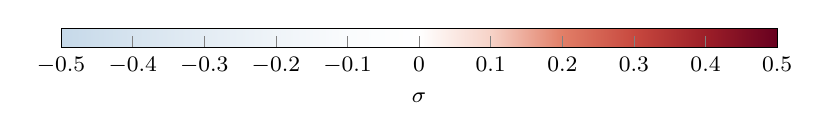
\begin{tikzpicture}
\begin{axis}[
hide axis, scale only axis,
width=0.75\textwidth, height=0pt,
colormap={sigmamap}{rgb(0.0000)=(0.7760,0.8510,0.9140); rgb(0.1000)=(0.8392,0.8918,0.9369); rgb(0.2000)=(0.8913,0.9259,0.9563); rgb(0.3000)=(0.9374,0.9569,0.9743); rgb(0.4000)=(0.9799,0.9861,0.9917); rgb(0.5000)=(1.0000,0.9999,0.9999); rgb(0.6000)=(0.9659,0.8254,0.7818); rgb(0.7000)=(0.8840,0.4951,0.4053); rgb(0.8000)=(0.7820,0.2849,0.2466); rgb(0.9000)=(0.6131,0.1208,0.1566); rgb(1.0000)=(0.4040,0.0000,0.1220)},
point meta min=-0.5, point meta max=0.5,
colorbar horizontal,
colorbar style={
  width=0.75\textwidth, height=7pt,
  at={(0,0)}, anchor=north west,
  xlabel={$\sigma$},
  xlabel style={font=\footnotesize},
  tick label style={font=\footnotesize},
  xtick pos=bottom,
},
]
\addplot[draw=none] coordinates {(0,0)};
\end{axis}
\end{tikzpicture}

  \caption{Per-wavenumber growth-rate fields in the Boussinesq limit for \(\Sch=1\) and
  \(\delta_0=2\). (a)~Non-autonomous mean growth rate \(\overline{\sigma}_{1D}(k,t)\), with the
  early-time window \(t\leq2\) shown in the inset. (b)~QSSA growth rate
  \(\sigma_{\mathrm{QSSA}}(k,t_0)\).}
  \label{fig:BQ_P3_sigma_map}
\end{figure}






\subsection{Three-dimensional perturbation growth}
From the family of spectra introduced in~\cref{sec:statistics_of_the_initial_perturbations}, we fix
\(n=1\), the simplest member, which corresponds to a Gaussian spatial correlation. The
higher-order spectra produce the same qualitative behaviour and are therefore omitted here so that
we can isolate the effect of the horizontal correlation length. Keeping the initial variance
\(\mean{\eta_0^2}\) fixed, we vary the integral correlation length \(\lambda\) of the \(n=1\)
spectrum defined in~\eqref{eq:eta_spectrum_family}. For this spectrum,
\(\lambda_0=2\lambda/\sqrt{\pi}\), where \(\lambda_0\) is the Gaussian reference scale defined in
\eqref{eq:lambda0_k0_relation}. The mean energy growth defined in~\eqref{eq:gmean_eta_spectrum}
therefore reduces, after switching to polar coordinates \((k,\theta)\) and integrating by parts, to
\begin{equation}
    \label{eq:bq_gmean_isotropic}
    \Gm(t)
    =
    g(0,t)
    +
    \int_{0}^{\infty}
    \frac{\partial g(k,t)}{\partial k}
    \exp\!\left(-\frac{\lambda^{2}k^{2}}{\pi}\right)\mathrm{d}k.
\end{equation}

\Cref{fig:compare_dns}(b) shows a representative evolution of \(\Gm(t)\) for a
fixed correlation length. The mean energy initially decays, reflecting the dominance of stable
contributions at early times. This decay continues until the minimum \(\Gm_{\min}(\lambda)\) is
reached. Beyond this point, the trajectory reverses and exhibits growth driven by the unstable
modes represented in the spectrum. A key feature of this behaviour is the delay before the mean
energy returns to its initial level. In terms of the quantities defined in
\eqref{eq:minimum_growth_critical_time_definitions}, \(\Gm_{\min}\) measures the maximum transient
energy loss, whereas \(t_c\) measures how long the perturbation takes to recover its initial mean
energy.

\begin{figure}
  \centering
  \begin{minipage}{0.48\textwidth}
    \centering
    % This file was created by matlab2tikz.
%
\definecolor{mycolor1}{rgb}{0.75000,0.08000,0.08000}%
\definecolor{mycolor2}{rgb}{0.83368,0.83368,0.83368}%
\definecolor{mycolor3}{rgb}{0.78737,0.78737,0.78737}%
\definecolor{mycolor4}{rgb}{0.74105,0.74105,0.74105}%
\definecolor{mycolor5}{rgb}{0.69474,0.69474,0.69474}%
\definecolor{mycolor6}{rgb}{0.64842,0.64842,0.64842}%
\definecolor{mycolor7}{rgb}{0.60211,0.60211,0.60211}%
\definecolor{mycolor8}{rgb}{0.50947,0.50947,0.50947}%
\definecolor{mycolor9}{rgb}{0.46316,0.46316,0.46316}%
%
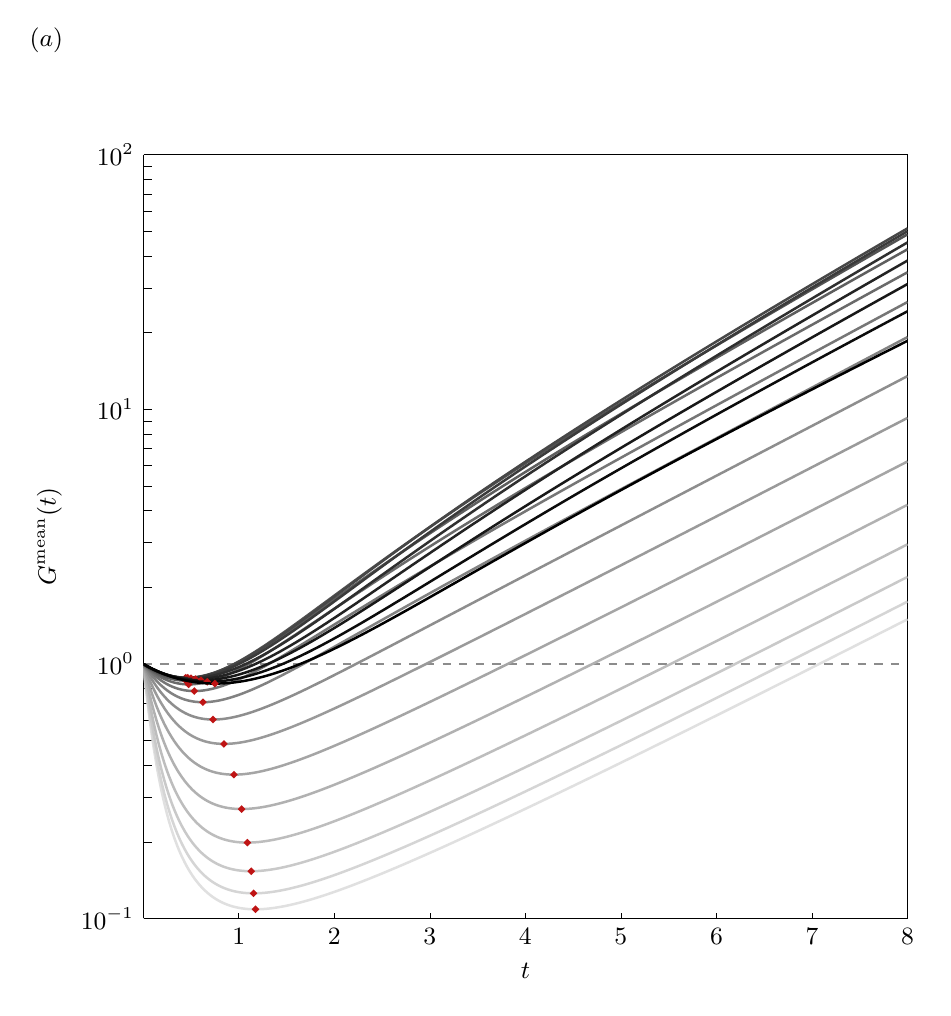
\begin{tikzpicture}

\begin{axis}[%
width=11.252in,
height=7.131in,
at={(1.887in,0.962in)},
scale only axis,
clip=true,
separate axis lines,
every outer x axis line/.append style={black},
every x tick label/.append style={font=\color{black}},
every x tick/.append style={black},
xmin=0.005,
xmax=8,
xlabel={$t$},
every outer y axis line/.append style={black},
every y tick label/.append style={font=\color{black}},
every y tick/.append style={black},
ymode=log,
ymin=0.1,
ymax=100,
yminorticks=true,
ylabel={$\mathscr{G}^{\mathrm{mean}}(t)$},
axis background/.style={fill=white},
clip=true,
clip mode=individual,
axis lines=box,
xtick pos=bottom,
ytick pos=left,
tick align=inside,
major tick length=2pt,
width=0.8\linewidth,
height=0.8\linewidth,
every axis/.append style={font=\fontsize{9}{9}\selectfont},xlabel style={font=\fontsize{9}{9}\selectfont},title style={font=\fontsize{9}{9}\selectfont},
legend style={font=\fontsize{8}{9}\selectfont,inner sep=1pt,row sep=1pt,column sep=2pt,nodes={scale=1.00},draw=none},legend image post style={xscale=0.35},
legend columns=1,
scaled x ticks=false,
tick label style={/pgf/number format/fixed,/pgf/number format/precision=2},
every x tick label/.append style={font=\fontsize{9}{9}\selectfont\color{black}},
every y tick label/.append style={font=\fontsize{9}{9}\selectfont\color{black}},
,,
colormap={sigmamap}{rgb(0.0000)=(0.0200,0.1880,0.3800); rgb(0.1000)=(0.0743,0.3456,0.5616); rgb(0.2000)=(0.1918,0.4980,0.7060); rgb(0.3000)=(0.3890,0.6708,0.8226); rgb(0.4000)=(0.7552,0.8682,0.9228); rgb(0.5000)=(0.9690,0.9689,0.9689); rgb(0.6000)=(0.9425,0.8044,0.7614); rgb(0.7000)=(0.8767,0.4910,0.4020); rgb(0.8000)=(0.7869,0.2866,0.2470); rgb(0.9000)=(0.6186,0.1239,0.1568); rgb(1.0000)=(0.4040,0.0000,0.1220)}
]
\addplot [color=white!55!black, dashed, line width=0.7pt, forget plot]
  table[row sep=crcr]{%
0.005	1\\
8	1\\
};
\addplot [color=white!88!black, line width=0.9pt, forget plot]
  table[row sep=crcr]{%
0.005	0.959051936801755\\
0.03	0.786622229327457\\
0.06	0.634528217945405\\
0.085	0.540096388507333\\
0.11	0.46667404537218\\
0.14	0.398746788498769\\
0.165	0.354524829253815\\
0.19	0.318695676138571\\
0.22	0.284098969809706\\
0.245	0.260638865906569\\
0.27	0.240970544521686\\
0.3	0.221314853434199\\
0.325	0.207557168028668\\
0.355	0.193552959443092\\
0.38	0.183586450015501\\
0.405	0.174896039567011\\
0.435	0.165870786594321\\
0.46	0.15933198135657\\
0.485	0.153549055135064\\
0.515	0.147461587181857\\
0.54	0.142999076105584\\
0.565	0.139016539204789\\
0.595	0.134789359848328\\
0.62	0.131669437223373\\
0.645	0.12887173268871\\
0.675	0.125890933092623\\
0.7	0.123685799654635\\
0.725	0.121706957760053\\
0.755	0.119600220215998\\
0.78	0.118045525724334\\
0.805	0.116655807448684\\
0.835	0.11518561448178\\
0.86	0.114110143165207\\
0.885	0.113158833833264\\
0.915	0.112167314561309\\
0.94	0.111455851055121\\
0.97	0.11072829471931\\
0.995	0.110219111163394\\
1.02	0.109791658689233\\
1.05	0.109378876680707\\
1.075	0.109112568650033\\
1.1	0.10891213100725\\
1.13	0.108752924365368\\
1.155	0.108683770989646\\
1.18	0.108668862142593\\
1.21	0.108718398088749\\
1.235	0.108812701218992\\
1.26	0.108952586010286\\
1.29	0.109177473426788\\
1.315	0.109410009553778\\
1.34	0.109681585253684\\
1.37	0.110056617017258\\
1.395	0.110408268474274\\
1.42	0.110793966202364\\
1.45	0.111299908584993\\
1.475	0.111756043151122\\
1.5	0.112242382286623\\
1.53	0.112864441011134\\
1.555	0.113413779524707\\
1.585	0.114108863521928\\
1.61	0.11471708588891\\
1.635	0.11535089579696\\
1.665	0.116144320338243\\
1.69	0.116832177355282\\
1.715	0.117543688643448\\
1.745	0.1184280118542\\
1.77	0.119189826327699\\
1.795	0.119973802103961\\
1.825	0.120943277414146\\
1.85	0.121774675606844\\
1.875	0.122627092107432\\
1.905	0.123677320132539\\
1.93	0.124574968490897\\
1.955	0.125492773722522\\
1.985	0.126620438678425\\
2.01	0.127581843743809\\
2.035	0.128562773448434\\
2.065	0.129765441470972\\
2.09	0.130788796268215\\
2.115	0.131831232222962\\
2.145	0.133107195599691\\
2.17	0.134191260638556\\
2.2	0.135516942366521\\
2.225	0.136642276446065\\
2.25	0.137786286793492\\
2.28	0.139183703282516\\
2.305	0.140368693422417\\
2.33	0.141572285620825\\
2.36	0.143041149397919\\
2.385	0.144285673838851\\
2.41	0.145548828080824\\
2.44	0.147089243678282\\
2.465	0.148393491592169\\
2.49	0.149716485732398\\
2.52	0.151328898624726\\
2.545	0.152693330731551\\
2.57	0.154076703563642\\
2.6	0.155761859345211\\
2.625	0.157187176396131\\
2.65	0.158631698241253\\
2.68	0.160390609908167\\
2.705	0.161877727410953\\
2.73	0.163384376522708\\
2.76	0.165218298218467\\
2.785	0.16676832615477\\
2.815	0.168654659839379\\
2.84	0.170248675742009\\
2.865	0.17186290230651\\
2.895	0.17382685254802\\
2.92	0.175486049222594\\
2.945	0.17716592782631\\
2.975	0.17920930384315\\
3	0.180935242154863\\
3.025	0.1826823810971\\
3.055	0.184807174351432\\
3.08	0.186601564252003\\
3.105	0.188417718589389\\
3.135	0.190626093826845\\
3.16	0.192490787511916\\
3.185	0.194377852749989\\
3.215	0.196672141093591\\
3.24	0.198609127769553\\
3.265	0.200569135077012\\
3.295	0.202951828842209\\
3.32	0.204963230844535\\
3.345	0.206998343549422\\
3.375	0.209472092511534\\
3.4	0.211560162567233\\
3.43	0.214098129649751\\
3.455	0.216240282638421\\
3.48	0.218407402104518\\
3.51	0.221041246486127\\
3.535	0.223264160173831\\
3.56	0.225512838115331\\
3.59	0.228245623259352\\
3.615	0.230551894358107\\
3.64	0.232884767354722\\
3.67	0.235719709845447\\
3.695	0.238112062823826\\
3.72	0.240531895414647\\
3.75	0.243472365732355\\
3.775	0.245953653655037\\
3.8	0.248463339347015\\
3.83	0.251512863293342\\
3.855	0.254086069181481\\
3.88	0.256688631961402\\
3.91	0.259850892666645\\
3.935	0.26251913132633\\
3.96	0.265217727626221\\
3.99	0.268496568083427\\
4.015	0.271263088359085\\
4.045	0.27462439113607\\
4.07	0.277460435515063\\
4.095	0.280328622932599\\
4.125	0.283813361630922\\
4.15	0.286753481533873\\
4.175	0.289726861304626\\
4.205	0.293339324711937\\
4.23	0.296387143302755\\
4.255	0.299469383665188\\
4.285	0.303214033670304\\
4.31	0.306373319623556\\
4.335	0.30956823550411\\
4.365	0.313449711617198\\
4.39	0.316724382989394\\
4.415	0.320035939967634\\
4.445	0.324059064200426\\
4.47	0.3274531925976\\
4.495	0.330885511163788\\
4.525	0.335055293257219\\
4.55	0.338573108288825\\
4.575	0.342130468386131\\
4.605	0.346452111375905\\
4.63	0.350098005387953\\
4.66	0.354527174172372\\
4.685	0.358263757344955\\
4.71	0.362042290428044\\
4.74	0.366632555134397\\
4.765	0.370505012477596\\
4.79	0.374420917746101\\
4.82	0.379178031017581\\
4.845	0.383191217802176\\
4.87	0.387249406943351\\
4.9	0.392179338075172\\
4.925	0.396338292116706\\
4.95	0.400543861209951\\
4.98	0.405652803243757\\
5.005	0.409962750907482\\
5.03	0.414320986514539\\
5.06	0.419615363659417\\
5.085	0.424081726138596\\
5.11	0.42859811166738\\
5.14	0.434084587049644\\
5.165	0.43871298691908\\
5.19	0.4433932092641\\
5.22	0.449078693011665\\
5.245	0.453874961060766\\
5.275	0.459701403853549\\
5.3	0.464616575190053\\
5.325	0.469586757540694\\
5.355	0.475624453277258\\
5.38	0.480717824371351\\
5.405	0.485868189885686\\
5.435	0.492124755214765\\
5.46	0.497402752513177\\
5.485	0.502739800497738\\
5.515	0.509223131863334\\
5.54	0.514692417729638\\
5.565	0.520222885942843\\
5.595	0.526941169321147\\
5.62	0.532608650255913\\
5.645	0.538339523227016\\
5.675	0.54530124423923\\
5.7	0.551174079417599\\
5.725	0.557112597084636\\
5.755	0.564326551496869\\
5.78	0.570412161631587\\
5.805	0.576565828307862\\
5.835	0.58404113292925\\
5.86	0.59034720946807\\
5.89	0.598007653054724\\
5.915	0.604469907136169\\
5.94	0.611004421804513\\
5.97	0.618942359922614\\
5.995	0.62563870040593\\
6.02	0.632409915103689\\
6.05	0.640635384574641\\
6.075	0.647574278786116\\
6.1	0.654590755851724\\
6.13	0.663114158361287\\
6.155	0.670304381339735\\
6.18	0.677574994190676\\
6.21	0.686407109217126\\
6.235	0.693857754621567\\
6.26	0.701391698785071\\
6.29	0.71054369699996\\
6.315	0.718264188415316\\
6.34	0.726070992961443\\
6.37	0.735554450119027\\
6.395	0.743554552773223\\
6.42	0.751644092162982\\
6.45	0.76147100349314\\
6.475	0.769760836398893\\
6.505	0.779831055753588\\
6.53	0.788326137884266\\
6.555	0.79691618642002\\
6.585	0.807351094918034\\
6.61	0.816153820651702\\
6.635	0.825054949596217\\
6.665	0.835867745217041\\
6.69	0.844989247974341\\
6.715	0.854212715010149\\
6.745	0.865417072922753\\
6.77	0.874868888591254\\
6.795	0.884426358292284\\
6.825	0.896036447844801\\
6.85	0.905830529111434\\
6.875	0.915734087433268\\
6.905	0.927764589752483\\
6.93	0.937913320945799\\
6.955	0.948175490233948\\
6.985	0.960641616452918\\
7.01	0.971157828919422\\
7.035	0.98179158345199\\
7.065	0.994709093590183\\
7.09	1.00560608161706\\
7.12	1.01884335481844\\
7.145	1.03001008621964\\
7.17	1.04130162352544\\
7.2	1.0550181751501\\
7.225	1.06658921222004\\
7.25	1.07828956903364\\
7.28	1.09250273306911\\
7.305	1.10449269760837\\
7.33	1.11661665835403\\
7.36	1.13134439329173\\
7.385	1.14376843381891\\
7.41	1.15633131543033\\
7.44	1.1715922265079\\
7.465	1.18446603701819\\
7.49	1.19748370790365\\
7.52	1.21329707013792\\
7.545	1.22663690952747\\
7.57	1.24012580920638\\
7.6	1.25651159124044\\
7.625	1.27033430341967\\
7.65	1.28431146285627\\
7.68	1.30129035165412\\
7.705	1.31561338637362\\
7.735	1.3330124216263\\
7.76	1.34768987544438\\
7.785	1.36253130985754\\
7.815	1.38056006167157\\
7.84	1.39576871873975\\
7.865	1.41114727972953\\
7.895	1.42982849478567\\
7.92	1.4455875420354\\
7.945	1.46152262932997\\
7.975	1.48087987148436\\
8	1.49720918505694\\
};
\addplot [color=mycolor1, line width=1.4pt, only marks, mark size=0.4pt, mark=*, mark options={solid, fill=mycolor1, mycolor1}, forget plot]
  table[row sep=crcr]{%
1.175	0.108667651227639\\
};
\addplot [color=mycolor2, line width=0.9pt, forget plot]
  table[row sep=crcr]{%
0.005	0.961707842717039\\
0.03	0.799460446285425\\
0.06	0.654646276767796\\
0.085	0.563645139599043\\
0.11	0.492129910071565\\
0.14	0.425214171316473\\
0.165	0.381170028601366\\
0.19	0.345150388287714\\
0.22	0.310037933930232\\
0.245	0.286016465240029\\
0.27	0.265730269316037\\
0.3	0.245310500935774\\
0.325	0.230924352181741\\
0.355	0.216196431151661\\
0.38	0.205661158619046\\
0.405	0.196437371813497\\
0.435	0.186820800469046\\
0.46	0.179829796995251\\
0.485	0.173630541747616\\
0.515	0.167088719904601\\
0.54	0.162283205266665\\
0.565	0.157988037693065\\
0.595	0.153423113413825\\
0.62	0.1500507354806\\
0.645	0.147025047234302\\
0.675	0.143800626219563\\
0.7	0.141415619918082\\
0.725	0.139276412771715\\
0.755	0.137001128315837\\
0.78	0.135324464279381\\
0.805	0.133828395776939\\
0.835	0.132249772299823\\
0.86	0.131098845276331\\
0.885	0.130084723755595\\
0.915	0.129033432135786\\
0.94	0.128284331827419\\
0.97	0.127525257490332\\
0.995	0.12700049330635\\
1.02	0.126566601181478\\
1.05	0.12615746884713\\
1.075	0.125903157108386\\
1.1	0.125722417917874\\
1.13	0.125596487074754\\
1.155	0.12556268994566\\
1.18	0.125589732203869\\
1.21	0.125697905866218\\
1.235	0.125847674035879\\
1.26	0.12604876194903\\
1.29	0.126354350022129\\
1.315	0.126659940532139\\
1.34	0.12700964281338\\
1.37	0.127484874562402\\
1.395	0.127925209520082\\
1.42	0.128404143902913\\
1.45	0.129027787549954\\
1.475	0.129586706068757\\
1.5	0.130179977356563\\
1.53	0.130935679911884\\
1.555	0.131600710582804\\
1.585	0.132439677017438\\
1.61	0.133171914364017\\
1.635	0.133933397328866\\
1.665	0.134884760496843\\
1.69	0.135708100861191\\
1.715	0.13655854959434\\
1.745	0.137614082569128\\
1.77	0.138522252544808\\
1.795	0.139455883074311\\
1.825	0.140609243307358\\
1.85	0.141597419615375\\
1.875	0.142609798679597\\
1.905	0.143856144879799\\
1.93	0.144920664367385\\
1.955	0.146008443347643\\
1.985	0.147344144674196\\
2.01	0.148482283388075\\
2.035	0.149642994968492\\
2.065	0.15106540803458\\
2.09	0.15227521125669\\
2.115	0.153507112545343\\
2.145	0.155014408855734\\
2.17	0.156294559195304\\
2.2	0.157859510122772\\
2.225	0.159187540987469\\
2.25	0.16053725520872\\
2.28	0.162185490426978\\
2.305	0.163582813599598\\
2.33	0.165001761373978\\
2.36	0.166733052471063\\
2.385	0.16819961080713\\
2.41	0.169687850355133\\
2.44	0.171502412486637\\
2.465	0.173038500947475\\
2.49	0.174596427810397\\
2.52	0.176494862804218\\
2.545	0.178101084566285\\
2.57	0.179729390673243\\
2.6	0.181712641520741\\
2.625	0.183389872836418\\
2.65	0.185089513710209\\
2.68	0.187158828083252\\
2.705	0.188908190097728\\
2.73	0.19068035854514\\
2.76	0.192837259523404\\
2.785	0.194660095662778\\
2.815	0.196878227663703\\
2.84	0.198752463272158\\
2.865	0.200650321126919\\
2.895	0.20295917130455\\
2.92	0.204909603384974\\
2.945	0.206884220247171\\
2.975	0.209285948240668\\
3	0.21131443769238\\
3.025	0.213367729084113\\
3.055	0.215864704392751\\
3.08	0.217973283916095\\
3.105	0.220107334584163\\
3.135	0.222702126656282\\
3.16	0.224892993195159\\
3.185	0.227110050154355\\
3.215	0.229805420786414\\
3.24	0.232080929781646\\
3.265	0.234383397072013\\
3.295	0.237182294745955\\
3.32	0.239544955911461\\
3.345	0.241935390800632\\
3.375	0.244840946659351\\
3.4	0.247293421049389\\
3.43	0.250274214341842\\
3.455	0.252790056681783\\
3.48	0.255335154861275\\
3.51	0.258428297593623\\
3.535	0.261038782222559\\
3.56	0.263679463387694\\
3.59	0.266888567845268\\
3.615	0.26959675606709\\
3.64	0.272336127992298\\
3.67	0.27566498494029\\
3.695	0.27847408702624\\
3.72	0.281315406735803\\
3.75	0.284767986499766\\
3.775	0.287681362809307\\
3.8	0.290628037890601\\
3.83	0.294208492177555\\
3.855	0.297229654872719\\
3.88	0.300285245363543\\
3.91	0.303997909747041\\
3.935	0.307130525041215\\
3.96	0.310298745835141\\
3.99	0.314148142842595\\
4.015	0.317396033735455\\
4.045	0.321342156719763\\
4.07	0.324671600211417\\
4.095	0.32803874967065\\
4.125	0.332129671362394\\
4.15	0.335581206357394\\
4.175	0.339071760914883\\
4.205	0.343312525713034\\
4.23	0.34689041348261\\
4.255	0.350508687219353\\
4.285	0.354904542329541\\
4.31	0.358613214648278\\
4.335	0.362363693547376\\
4.365	0.366920094352327\\
4.39	0.370764158094212\\
4.415	0.374651504745458\\
4.445	0.379374120591656\\
4.47	0.383358362668924\\
4.495	0.387387421311852\\
4.525	0.392282141698599\\
4.55	0.396411534332348\\
4.575	0.400587336229311\\
4.605	0.405660277389791\\
4.63	0.409939983704711\\
4.66	0.415139120688698\\
4.685	0.419525264702665\\
4.71	0.423960644641303\\
4.74	0.429348857276454\\
4.765	0.433894477268899\\
4.79	0.438491093821522\\
4.82	0.444075143262269\\
4.845	0.448785945595956\\
4.87	0.453549571344957\\
4.9	0.459336473043973\\
4.925	0.464218378356061\\
4.95	0.469155002335518\\
4.98	0.47515203440512\\
5.005	0.480211184683509\\
5.03	0.485327019555136\\
5.06	0.49154173151017\\
5.085	0.496784497489258\\
5.11	0.502085987038125\\
5.14	0.508526208923197\\
5.165	0.513959197801442\\
5.19	0.5194530247552\\
5.22	0.526126876663319\\
5.245	0.531756940147906\\
5.275	0.538596278447651\\
5.3	0.544365936312634\\
5.325	0.550200178997572\\
5.355	0.557287535513878\\
5.38	0.563266408197994\\
5.405	0.56931219628188\\
5.435	0.57665652087574\\
5.46	0.582852159667638\\
5.485	0.589117130018651\\
5.515	0.596727701192433\\
5.54	0.603147934488745\\
5.565	0.609640004065366\\
5.595	0.617526440417675\\
5.62	0.624179383393132\\
5.645	0.63090675903014\\
5.675	0.639079031151612\\
5.7	0.645973095801507\\
5.725	0.652944284370212\\
5.755	0.661412727193457\\
5.78	0.668556632758011\\
5.805	0.675780451712034\\
5.835	0.684555777328928\\
5.86	0.691958561110103\\
5.89	0.700951284844929\\
5.915	0.708537460386625\\
5.94	0.716208488970245\\
5.97	0.725527064690993\\
5.995	0.733388121603641\\
6.02	0.741337102497315\\
6.05	0.750993323188234\\
6.075	0.759139210337827\\
6.1	0.767376204040185\\
6.13	0.777382291375649\\
6.155	0.785823319172165\\
6.18	0.794358751684204\\
6.21	0.804727371229734\\
6.235	0.8134742244523\\
6.26	0.822318900247047\\
6.29	0.833063177215489\\
6.315	0.842126928305107\\
6.34	0.851292043770011\\
6.37	0.862425579351784\\
6.395	0.871817702187386\\
6.42	0.881314859554296\\
6.45	0.892851747839197\\
6.475	0.902584132012682\\
6.505	0.914406765471842\\
6.53	0.924380199303951\\
6.555	0.93446516491121\\
6.585	0.946716101712322\\
6.61	0.9570508447111\\
6.635	0.967501157676142\\
6.665	0.98019590523176\\
6.69	0.990905039002894\\
6.715	1.00173392695296\\
6.745	1.01488855342639\\
6.77	1.02598563252144\\
6.795	1.03720680123111\\
6.825	1.05083795550971\\
6.85	1.06233702427548\\
6.875	1.07396467470153\\
6.905	1.08808960708677\\
6.93	1.10000521711383\\
6.955	1.1120540630389\\
6.985	1.12669064667458\\
7.01	1.1390378748736\\
7.035	1.15152316117799\\
7.065	1.16668991424552\\
7.09	1.17948438156571\\
7.12	1.19502671429192\\
7.145	1.20813801185707\\
7.17	1.22139590267231\\
7.2	1.23750118138974\\
7.225	1.25108736644192\\
7.25	1.26482544862835\\
7.28	1.2815140412461\\
7.305	1.29559229483457\\
7.33	1.30982794056056\\
7.36	1.32712094891931\\
7.385	1.34170907110682\\
7.41	1.3564602783625\\
7.44	1.37437956438184\\
7.465	1.38949599629659\\
7.49	1.40478141118856\\
7.52	1.42334962394382\\
7.545	1.43901347061414\\
7.57	1.45485241044957\\
7.6	1.47409301420562\\
7.625	1.49032406820445\\
7.65	1.50673654539469\\
7.68	1.52667384863613\\
7.705	1.54349261456327\\
7.735	1.56392345259\\
7.76	1.581158546861\\
7.785	1.59858626669145\\
7.815	1.61975682339029\\
7.84	1.63761591675999\\
7.865	1.65567459609065\\
7.895	1.67761160070464\\
7.92	1.69611723946488\\
7.945	1.71482967468857\\
7.975	1.73756081689083\\
8	1.75673635736723\\
};
\addplot [color=mycolor1, line width=1.4pt, only marks, mark size=0.4pt, mark=*, mark options={solid, fill=mycolor1, mycolor1}, forget plot]
  table[row sep=crcr]{%
1.155	0.12556268994566\\
};
\addplot [color=mycolor3, line width=0.9pt, forget plot]
  table[row sep=crcr]{%
0.005	0.965582581329303\\
0.03	0.818326278313415\\
0.06	0.684460688031333\\
0.085	0.598781461558633\\
0.11	0.530360135731492\\
0.14	0.465259657383791\\
0.165	0.421720303451766\\
0.19	0.385632718155537\\
0.22	0.349976127793189\\
0.245	0.325277056364376\\
0.27	0.304205776160398\\
0.3	0.282783266203527\\
0.325	0.267554638698581\\
0.355	0.251841984789343\\
0.38	0.240524045723158\\
0.405	0.230560465539586\\
0.435	0.220118157844473\\
0.46	0.212492346807002\\
0.485	0.205706523723853\\
0.515	0.198522753167361\\
0.54	0.19323175896303\\
0.565	0.188493810949771\\
0.595	0.183450691846933\\
0.62	0.179721386168037\\
0.645	0.176374134778945\\
0.675	0.172807447797278\\
0.7	0.170171134416928\\
0.725	0.167809379211337\\
0.755	0.165302455530153\\
0.78	0.163460306622273\\
0.805	0.161822142009088\\
0.835	0.160101868430468\\
0.86	0.15885541252102\\
0.885	0.157764938902782\\
0.915	0.156645779330961\\
0.94	0.155858723917831\\
0.97	0.15507503191264\\
0.995	0.154546193231645\\
1.02	0.154122336643403\\
1.05	0.15374286224222\\
1.075	0.15352717088063\\
1.1	0.153397046139891\\
1.13	0.153346901716747\\
1.155	0.153388200054875\\
1.18	0.153500689464753\\
1.21	0.153724454670675\\
1.235	0.153980960342441\\
1.26	0.154297858374241\\
1.29	0.154753919006989\\
1.315	0.155194121581695\\
1.34	0.155686509756298\\
1.37	0.156343250350273\\
1.395	0.156943128419968\\
1.42	0.157588898805006\\
1.45	0.158422081701795\\
1.475	0.159163173035899\\
1.5	0.159945299866474\\
1.53	0.160936223686182\\
1.555	0.161804260414313\\
1.585	0.162895017026846\\
1.61	0.163843752824848\\
1.635	0.164827679229792\\
1.665	0.166053675329918\\
1.69	0.167112182022827\\
1.715	0.168203436587606\\
1.745	0.169555269548493\\
1.77	0.170716382814763\\
1.795	0.171908366054209\\
1.825	0.173378807757287\\
1.85	0.174637038902254\\
1.875	0.175924713929306\\
1.905	0.177508275233884\\
1.93	0.178859481086184\\
1.955	0.180239070407503\\
1.985	0.181931669356999\\
2.01	0.183372799913474\\
2.035	0.184841552929916\\
2.065	0.186640259508985\\
2.09	0.188169163195523\\
2.115	0.189725176298128\\
2.145	0.191628014361183\\
2.17	0.193243286491934\\
2.2	0.195216989065666\\
2.225	0.196891155093106\\
2.25	0.198592019068112\\
2.28	0.200668265625047\\
2.305	0.202427804374581\\
2.33	0.204214017940533\\
2.36	0.206392716427014\\
2.385	0.208237708882683\\
2.41	0.210109489761308\\
2.44	0.212391073848133\\
2.465	0.214322018810009\\
2.49	0.216279985426423\\
2.52	0.218665348658474\\
2.545	0.220683111929097\\
2.57	0.222728236012066\\
2.6	0.225218679099735\\
2.625	0.227324452779959\\
2.65	0.229458021371213\\
2.68	0.23205520992505\\
2.705	0.234250479764952\\
2.73	0.236474064742888\\
2.76	0.239179995370398\\
2.785	0.241466514586513\\
2.815	0.244248522400411\\
2.84	0.246598921384243\\
2.865	0.248978689706051\\
2.895	0.251873486391828\\
2.92	0.254318643468047\\
2.945	0.256793890443779\\
2.975	0.259804242386666\\
3	0.262346537262013\\
3.025	0.264919709059013\\
3.055	0.268048637980242\\
3.08	0.2706906596119\\
3.105	0.273364408704069\\
3.135	0.276615180335525\\
3.16	0.279359718316624\\
3.185	0.282136895575239\\
3.215	0.285513011046204\\
3.24	0.288363049118826\\
3.265	0.291246697918424\\
3.295	0.294751887422836\\
3.32	0.297710598784046\\
3.345	0.300703950810983\\
3.375	0.304342169206298\\
3.4	0.307412913337745\\
3.43	0.311144998607249\\
3.455	0.314294809904984\\
3.48	0.317481130707315\\
3.51	0.32135342115034\\
3.535	0.3246213521029\\
3.56	0.327926977156956\\
3.59	0.331944021652232\\
3.615	0.335333926207669\\
3.64	0.338762767018086\\
3.67	0.342929335501002\\
3.695	0.346445252205777\\
3.72	0.350001405308359\\
3.75	0.354322490427705\\
3.775	0.357968644070841\\
3.8	0.361656392906895\\
3.83	0.36613721256776\\
3.855	0.369918016535818\\
3.88	0.373741834014711\\
3.91	0.378387834718158\\
3.935	0.382307893992205\\
3.96	0.386272445676783\\
3.99	0.391089306584425\\
4.015	0.395153421322757\\
4.045	0.400091166128116\\
4.07	0.404257206849303\\
4.095	0.408470376510162\\
4.125	0.413589106160734\\
4.15	0.417907756925516\\
4.175	0.422275184892209\\
4.205	0.427581228963454\\
4.23	0.432057836283208\\
4.255	0.436584934961904\\
4.285	0.442084876086223\\
4.31	0.446724999261526\\
4.335	0.451417395627863\\
4.365	0.457118076329944\\
4.39	0.461927493294284\\
4.415	0.466791034869924\\
4.445	0.472699564911519\\
4.47	0.477684278494932\\
4.495	0.482725039739063\\
4.525	0.488848803957546\\
4.55	0.494015048557714\\
4.575	0.499239337664187\\
4.605	0.50558600429328\\
4.63	0.510940252945601\\
4.66	0.517444764623541\\
4.685	0.522932148501024\\
4.71	0.528481120342875\\
4.74	0.535222141937508\\
4.765	0.540909015235479\\
4.79	0.546659683360555\\
4.82	0.553645689620336\\
4.845	0.559539204785864\\
4.87	0.565498804487982\\
4.9	0.572738588311337\\
4.925	0.578846165886128\\
4.95	0.58502220329387\\
4.98	0.592524886252033\\
5.005	0.598854223776225\\
5.03	0.605254484880469\\
5.06	0.613029528214293\\
5.085	0.61958860952725\\
5.11	0.626221169606315\\
5.14	0.634278385701133\\
5.165	0.641075490642672\\
5.19	0.647948724090128\\
5.22	0.656298288437991\\
5.245	0.663342002957037\\
5.275	0.671898653951083\\
5.3	0.679117057175355\\
5.325	0.68641628385425\\
5.355	0.695283312577003\\
5.38	0.702763537830423\\
5.405	0.710327506833005\\
5.435	0.719516127760996\\
5.46	0.727267636995012\\
5.485	0.735105917448171\\
5.515	0.744627756631591\\
5.54	0.752660358843097\\
5.565	0.760782870662671\\
5.595	0.770649980103877\\
5.62	0.778973843472769\\
5.645	0.787390869645947\\
5.675	0.797615742229105\\
5.7	0.806241406721312\\
5.725	0.814963606056918\\
5.755	0.825559191045535\\
5.78	0.83449758149366\\
5.805	0.843536001854691\\
5.835	0.854515720973748\\
5.86	0.86377816064868\\
5.89	0.875030011120754\\
5.915	0.8845220167996\\
5.94	0.894120241489327\\
5.97	0.905779993390774\\
5.995	0.915616099295723\\
6.02	0.925562271904632\\
6.05	0.937644701102006\\
6.075	0.947837372528829\\
6.1	0.958144098217002\\
6.13	0.970664517681856\\
6.155	0.981226672910074\\
6.18	0.991907014786238\\
6.21	1.00488129366136\\
6.235	1.01582632004023\\
6.26	1.02689381542874\\
6.29	1.04033839878978\\
6.315	1.05168016940996\\
6.34	1.06314884670992\\
6.37	1.07708077604615\\
6.395	1.08883366701686\\
6.42	1.10071806317221\\
6.45	1.11515499760841\\
6.475	1.12733390595982\\
6.505	1.14212860654091\\
6.53	1.15460932284749\\
6.555	1.16722968507967\\
6.585	1.18256065273901\\
6.61	1.19549375841316\\
6.635	1.20857156971305\\
6.665	1.22445823465056\\
6.69	1.23786012048187\\
6.715	1.25141195463089\\
6.745	1.26787444977026\\
6.77	1.28176209924098\\
6.795	1.2958051292358\\
6.825	1.31286431527067\\
6.85	1.32725532568444\\
6.875	1.34180734509815\\
6.905	1.35948483643673\\
6.93	1.37439744079838\\
6.955	1.38947688590492\\
6.985	1.40779507754001\\
7.01	1.42324816722228\\
7.035	1.4388741399083\\
7.065	1.45785623524882\\
7.09	1.47386938346423\\
7.12	1.49332180626453\\
7.145	1.50973171465407\\
7.17	1.52632520076369\\
7.2	1.54648259699101\\
7.225	1.56348720800344\\
7.25	1.58068204269272\\
7.28	1.60156993406728\\
7.305	1.6191907762398\\
7.33	1.63700872758747\\
7.36	1.65865355571202\\
7.385	1.67691293343433\\
7.41	1.6953765539087\\
7.44	1.717805713055\\
7.465	1.73672673422069\\
7.49	1.75585938863527\\
7.52	1.77910125969621\\
7.545	1.79870786433544\\
7.57	1.81853375879445\\
7.6	1.84261774443602\\
7.625	1.86293473436371\\
7.65	1.88347894623522\\
7.68	1.90843550729792\\
7.705	1.92948857681242\\
7.735	1.95506327104373\\
7.76	1.97663777894933\\
7.785	1.99845354661724\\
7.815	2.02495472411759\\
7.84	2.04731078364516\\
7.865	2.06991682521254\\
7.895	2.09737798115924\\
7.92	2.12054384580851\\
7.945	2.14396872827512\\
7.975	2.17242456173868\\
8	2.19642950038594\\
};
\addplot [color=mycolor1, line width=1.4pt, only marks, mark size=0.4pt, mark=*, mark options={solid, fill=mycolor1, mycolor1}, forget plot]
  table[row sep=crcr]{%
1.13	0.153346901716747\\
};
\addplot [color=mycolor4, line width=0.9pt, forget plot]
  table[row sep=crcr]{%
0.005	0.970872099258847\\
0.03	0.84436814636939\\
0.06	0.726149097399875\\
0.085	0.648419077990237\\
0.11	0.584901552846846\\
0.14	0.52303012939518\\
0.165	0.48073041883824\\
0.19	0.445027928732667\\
0.22	0.409110799326526\\
0.245	0.383820426186479\\
0.27	0.361957401880175\\
0.3	0.339442001133725\\
0.325	0.32325164159219\\
0.355	0.306380206200183\\
0.38	0.294120970048508\\
0.405	0.283254543071193\\
0.435	0.271792314916088\\
0.46	0.263375395623777\\
0.485	0.255854409790341\\
0.515	0.247862884487803\\
0.54	0.241959911168704\\
0.565	0.236663965583826\\
0.595	0.231019708396329\\
0.62	0.226843878542514\\
0.645	0.223097068540184\\
0.675	0.219109556901465\\
0.7	0.216168682186811\\
0.725	0.213541884069224\\
0.755	0.210766035233564\\
0.78	0.20873832327656\\
0.805	0.206947582196063\\
0.835	0.205085231644008\\
0.86	0.203752591675302\\
0.885	0.20260355576056\\
0.915	0.201448549967696\\
0.94	0.200658742312173\\
0.97	0.199902442068615\\
0.995	0.19942067088987\\
1.02	0.199064793906225\\
1.05	0.198793130298012\\
1.075	0.198688089223346\\
1.1	0.198686644555774\\
1.13	0.198813637685341\\
1.155	0.199020654812187\\
1.18	0.199314623488634\\
1.21	0.199776119266107\\
1.235	0.200246709719914\\
1.26	0.200791666930823\\
1.29	0.201539177190986\\
1.315	0.202236555784066\\
1.34	0.202998689254124\\
1.37	0.203995190899594\\
1.395	0.204891188214158\\
1.42	0.205844543462526\\
1.45	0.207061551525301\\
1.475	0.208134450524823\\
1.5	0.209258986919441\\
1.53	0.210674476168237\\
1.555	0.211907466678214\\
1.585	0.213449260301259\\
1.61	0.214784565312426\\
1.635	0.216164621836789\\
1.665	0.217878389142645\\
1.69	0.219353561709496\\
1.715	0.22087061669706\\
1.745	0.222745314183006\\
1.77	0.224351952323476\\
1.795	0.225998279098023\\
1.825	0.228025462757544\\
1.85	0.229757171494328\\
1.875	0.231526918239819\\
1.905	0.233700234448067\\
1.93	0.235552239210275\\
1.955	0.237441073297052\\
1.985	0.239755868933544\\
2.01	0.241724718535085\\
2.035	0.243729552475905\\
2.065	0.246182573620641\\
2.09	0.248265910046099\\
2.115	0.250384688553607\\
2.145	0.252973845733556\\
2.17	0.255170224307426\\
2.2	0.257852278585556\\
2.225	0.260125941541563\\
2.25	0.262434689485689\\
2.28	0.265251499649749\\
2.305	0.267637458058415\\
2.33	0.270058562582784\\
2.36	0.273010359495041\\
2.385	0.275509001521877\\
2.41	0.278043020841298\\
2.44	0.281130689129318\\
2.465	0.283742923429267\\
2.49	0.286390915729788\\
2.52	0.289615914834822\\
2.545	0.292343109607197\\
2.57	0.29510657618078\\
2.6	0.298470877110247\\
2.625	0.301314811249556\\
2.65	0.30419565089948\\
2.68	0.30770168550432\\
2.705	0.31066450942348\\
2.73	0.313664981902643\\
2.76	0.317315602218387\\
2.785	0.320399806463086\\
2.815	0.324151686425611\\
2.84	0.327320948938009\\
2.865	0.330529339122381\\
2.895	0.334431483000966\\
2.92	0.337727032555457\\
2.945	0.341062709463031\\
2.975	0.345118955357877\\
3	0.348544086364364\\
3.025	0.352010430300225\\
3.055	0.356224946304535\\
3.08	0.359783224017916\\
3.105	0.363383882684019\\
3.135	0.367761153618179\\
3.16	0.371456404091417\\
3.185	0.37519528340407\\
3.215	0.379740100873513\\
3.24	0.38357640352088\\
3.265	0.387457660902947\\
3.295	0.392175116159921\\
3.32	0.396156798527242\\
3.345	0.400184838298342\\
3.375	0.405080317486486\\
3.4	0.409211951903104\\
3.43	0.414233098815328\\
3.455	0.418470603904285\\
3.48	0.422757005752241\\
3.51	0.427965927693774\\
3.535	0.432361651556273\\
3.56	0.436807878941188\\
3.59	0.442210745944892\\
3.615	0.446769914011867\\
3.64	0.45138126866068\\
3.67	0.456984543785531\\
3.695	0.461712626362028\\
3.72	0.466494655603757\\
3.75	0.472305097724052\\
3.775	0.477207812645432\\
3.8	0.482166312357634\\
3.83	0.488190980069646\\
3.855	0.493274296255456\\
3.88	0.498415314681008\\
3.91	0.504661571218733\\
3.935	0.509931713040875\\
3.96	0.515261555395891\\
3.99	0.521737074468989\\
4.015	0.527200526866232\\
4.045	0.533838279803104\\
4.07	0.539438533158014\\
4.095	0.545102047441598\\
4.125	0.551982735348573\\
4.15	0.557787849960571\\
4.175	0.563658450265698\\
4.205	0.570790616581771\\
4.23	0.576807808213267\\
4.255	0.582892798560887\\
4.285	0.590285325665049\\
4.31	0.596522095158257\\
4.335	0.602829067098818\\
4.365	0.61049118571582\\
4.39	0.616955327023041\\
4.415	0.623492167839953\\
4.445	0.631433467110158\\
4.47	0.638133075872193\\
4.495	0.644907977327526\\
4.525	0.653138415522818\\
4.55	0.66008189818114\\
4.575	0.667103365793281\\
4.605	0.675633281665995\\
4.63	0.682829365099291\\
4.66	0.691571372594439\\
4.685	0.698946352698278\\
4.71	0.706404094378674\\
4.74	0.715463922634622\\
4.765	0.723106985292293\\
4.79	0.730835783957229\\
4.82	0.740224855324537\\
4.845	0.748145640351917\\
4.87	0.756155247192158\\
4.9	0.765885411725457\\
4.925	0.774093919384788\\
4.95	0.782394449751495\\
4.98	0.792477999472462\\
5.005	0.800984602537482\\
5.03	0.809586548172125\\
5.06	0.820036231963563\\
5.085	0.828851688313587\\
5.11	0.837765930107868\\
5.14	0.848594969245373\\
5.165	0.85773043499371\\
5.19	0.866968256287049\\
5.22	0.878190360621641\\
5.245	0.887657403788438\\
5.275	0.89915795516936\\
5.3	0.908859889014843\\
5.325	0.918670503756016\\
5.355	0.930588410860061\\
5.38	0.94064241711989\\
5.405	0.950809038523604\\
5.435	0.963159409600786\\
5.46	0.973578235388201\\
5.485	0.98411375485242\\
5.515	0.99691225223288\\
5.54	1.00770911188851\\
5.565	1.01862689309467\\
5.595	1.03188975260864\\
5.62	1.04307834409254\\
5.645	1.05439223959204\\
5.675	1.06813629072988\\
5.7	1.0797308126387\\
5.725	1.09145518106796\\
5.755	1.10569786790317\\
5.78	1.11771303712915\\
5.805	1.12986276107278\\
5.835	1.14462216397083\\
5.86	1.15707323402088\\
5.89	1.17219870864921\\
5.915	1.18495859667679\\
5.94	1.19786137667374\\
5.97	1.21353558398058\\
5.995	1.22675838323648\\
6.02	1.24012925762063\\
6.05	1.25637210191452\\
6.075	1.27007460417526\\
6.1	1.28393055313273\\
6.13	1.30076266225012\\
6.155	1.31496226951303\\
6.18	1.32932089014944\\
6.21	1.34676364117914\\
6.235	1.3614783873653\\
6.26	1.37635791565249\\
6.29	1.39443346159663\\
6.315	1.40968203504258\\
6.34	1.42510136856287\\
6.37	1.44383266596644\\
6.395	1.45963443273161\\
6.42	1.47561315424497\\
6.45	1.49502399182395\\
6.475	1.51139901984031\\
6.505	1.53129128722176\\
6.53	1.54807245000698\\
6.555	1.5650415341\\
6.585	1.5856554553136\\
6.61	1.60304540570555\\
6.635	1.62063009351544\\
6.665	1.64199184370744\\
6.69	1.66001266242538\\
6.715	1.67823528125914\\
6.745	1.70037198251992\\
6.77	1.71904654896565\\
6.795	1.7379302336104\\
6.825	1.76086998875669\\
6.85	1.78022200951263\\
6.875	1.79979073104711\\
6.905	1.82356265861528\\
6.93	1.84361669695517\\
6.955	1.86389529259025\\
6.985	1.88852956307731\\
7.01	1.90931106953784\\
7.035	1.93032527351862\\
7.065	1.95585314691962\\
7.09	1.97738849095766\\
7.12	2.00354943434293\\
7.145	2.02561883125252\\
7.17	2.04793533403094\\
7.2	2.07504521110057\\
7.225	2.09791511970998\\
7.25	2.12104108805256\\
7.28	2.14913428332655\\
7.305	2.17283370842145\\
7.33	2.19679846997232\\
7.36	2.22591060780505\\
7.385	2.25046959988747\\
7.41	2.27530353952106\\
7.44	2.30547152832063\\
7.465	2.33092122090249\\
7.49	2.3566558184275\\
7.52	2.38791789644706\\
7.545	2.41429054466725\\
7.57	2.44095841386553\\
7.6	2.47335419661302\\
7.625	2.50068321722407\\
7.65	2.52831814627569\\
7.68	2.5618886756087\\
7.705	2.59020868838046\\
7.735	2.6246114289798\\
7.76	2.65363347667586\\
7.785	2.68298034726407\\
7.815	2.71863046948335\\
7.84	2.74870477834946\\
7.865	2.77911566268384\\
7.895	2.81605829861614\\
7.92	2.84722293820552\\
7.945	2.8787363284466\\
7.975	2.9170182330685\\
8	2.94931264170054\\
};
\addplot [color=mycolor1, line width=1.4pt, only marks, mark size=0.4pt, mark=*, mark options={solid, fill=mycolor1, mycolor1}, forget plot]
  table[row sep=crcr]{%
1.09	0.198675168593949\\
};
\addplot [color=mycolor5, line width=0.9pt, forget plot]
  table[row sep=crcr]{%
0.005	0.977212300208905\\
0.03	0.876116473648082\\
0.06	0.777970765986068\\
0.085	0.711078575945561\\
0.11	0.654762331237564\\
0.14	0.598250476224996\\
0.165	0.558550896556022\\
0.19	0.524296627244214\\
0.22	0.489086707104119\\
0.245	0.463811378605152\\
0.27	0.44162207032704\\
0.3	0.418428945121897\\
0.325	0.401531470453929\\
0.355	0.383725238271462\\
0.38	0.370660577421427\\
0.405	0.358993325863222\\
0.435	0.346601579341817\\
0.46	0.337450497794626\\
0.485	0.329240498847976\\
0.515	0.320488397708855\\
0.54	0.314009865274923\\
0.565	0.30819249298663\\
0.595	0.301993988551332\\
0.62	0.297415011045564\\
0.645	0.293317169666882\\
0.675	0.288975076606471\\
0.7	0.285792262023611\\
0.725	0.282970270869596\\
0.755	0.280019289736618\\
0.78	0.277892717227297\\
0.805	0.27604398575272\\
0.835	0.274163526253946\\
0.86	0.272856718772897\\
0.885	0.271769004109867\\
0.915	0.270732286924046\\
0.94	0.270076618728665\\
0.97	0.269521944329158\\
0.995	0.269240592735811\\
1.02	0.269113323492496\\
1.05	0.269151640447335\\
1.075	0.269333413458741\\
1.1	0.269643660551609\\
1.13	0.270176260684679\\
1.155	0.270746618438265\\
1.18	0.27142613084808\\
1.21	0.272378573668297\\
1.235	0.273281080552667\\
1.26	0.274278013297114\\
1.29	0.275593563436238\\
1.315	0.276785074637812\\
1.34	0.278059692494572\\
1.37	0.27969475877505\\
1.395	0.281142052034368\\
1.42	0.282663705272136\\
1.45	0.284584609965706\\
1.475	0.286261985151827\\
1.5	0.288006942808361\\
1.53	0.290187594017219\\
1.555	0.292075134316837\\
1.585	0.294422338193052\\
1.61	0.296445196310896\\
1.635	0.298527490149893\\
1.665	0.301103081344923\\
1.69	0.303312206019396\\
1.715	0.305577395226815\\
1.745	0.308368397824635\\
1.77	0.310753946402335\\
1.795	0.313193008916274\\
1.825	0.316189605260579\\
1.85	0.318744180234661\\
1.875	0.32135038377521\\
1.905	0.324545316013359\\
1.93	0.327263509407044\\
1.955	0.33003199136236\\
1.985	0.333420099841996\\
2.01	0.336298140743073\\
2.035	0.339225582328245\\
2.065	0.342803446602061\\
2.09	0.34583892632413\\
2.115	0.348923297925906\\
2.145	0.35268895550945\\
2.17	0.355880611780103\\
2.2	0.359774888826654\\
2.225	0.363073697212174\\
2.25	0.366421243675847\\
2.28	0.370502712655474\\
2.305	0.373957708934133\\
2.33	0.377461699760991\\
2.36	0.381731340821399\\
2.385	0.385343592993144\\
2.41	0.389005314915999\\
2.44	0.393464949075241\\
2.465	0.397236196302199\\
2.49	0.401057582257528\\
2.52	0.405709775372223\\
2.545	0.409642353821056\\
2.57	0.413625913739089\\
2.6	0.41847389951593\\
2.625	0.422570682894864\\
2.65	0.426719448204285\\
2.68	0.431767066479078\\
2.705	0.436031418385906\\
2.73	0.440348897565748\\
2.76	0.44560054491112\\
2.785	0.450036280741783\\
2.815	0.455431018624265\\
2.84	0.459987014195093\\
2.865	0.464598370846096\\
2.895	0.470205713715265\\
2.92	0.474940474831603\\
2.945	0.479732086800528\\
2.975	0.485557754583104\\
3	0.490476178016733\\
3.025	0.495453058792852\\
3.055	0.501503219805419\\
3.08	0.506610571126498\\
3.105	0.511778098985557\\
3.135	0.518059354498343\\
3.16	0.523361256477842\\
3.185	0.528725163971934\\
3.215	0.535244536953446\\
3.24	0.540746961254334\\
3.265	0.546313327824487\\
3.295	0.553078255230218\\
3.32	0.55878751689285\\
3.345	0.564562764141958\\
3.375	0.571581092229715\\
3.4	0.577503846551629\\
3.43	0.584701150681505\\
3.455	0.590774718055703\\
3.48	0.596917959540016\\
3.51	0.604382828343009\\
3.535	0.610681888690052\\
3.56	0.617052951796555\\
3.59	0.624794327421153\\
3.615	0.631326450189106\\
3.64	0.637933011672288\\
3.67	0.645960248388202\\
3.695	0.652733347753705\\
3.72	0.659583430409954\\
3.75	0.667906299643418\\
3.775	0.674928639142348\\
3.8	0.68203061682139\\
3.83	0.690659313656618\\
3.855	0.69793951199501\\
3.88	0.705302115758027\\
3.91	0.714247266770981\\
3.935	0.721794304713505\\
3.96	0.729426630040183\\
3.99	0.738699302357892\\
4.015	0.746522530610324\\
4.045	0.756027027409403\\
4.07	0.764045757074586\\
4.095	0.772154905092662\\
4.125	0.782006626888906\\
4.15	0.790318190021379\\
4.175	0.798723375690887\\
4.205	0.808934627061295\\
4.23	0.817549414639613\\
4.255	0.826261154784793\\
4.285	0.836844723591012\\
4.31	0.845773533219371\\
4.335	0.854802754905847\\
4.365	0.865771926177359\\
4.39	0.875025973918723\\
4.415	0.884384026524828\\
4.445	0.895752597255497\\
4.47	0.905343530219954\\
4.495	0.915042198256319\\
4.525	0.926824493094003\\
4.55	0.936764402766184\\
4.575	0.946815919432989\\
4.605	0.959026807248296\\
4.63	0.96932824354409\\
4.66	0.981842705273635\\
4.685	0.992400216340342\\
4.71	1.00307620238944\\
4.74	1.01604563140752\\
4.765	1.02698692815798\\
4.79	1.03805097580918\\
4.82	1.05149179242056\\
4.845	1.06283073206911\\
4.87	1.0742968581216\\
4.9	1.08822609547125\\
4.925	1.09997705176643\\
4.95	1.11185979493307\\
4.98	1.12629511966534\\
5.005	1.13847300035933\\
5.03	1.15078743896944\\
5.06	1.16574717278036\\
5.085	1.17836743784778\\
5.11	1.1911292083011\\
5.14	1.20663235039504\\
5.165	1.21971103101005\\
5.19	1.23293634699415\\
5.22	1.2490025974656\\
5.245	1.26255631575325\\
5.275	1.27902150667106\\
5.3	1.29291177239627\\
5.325	1.30695776197573\\
5.355	1.32402096275601\\
5.38	1.33841571366332\\
5.405	1.3529718410006\\
5.435	1.370654758597\\
5.46	1.38557230905067\\
5.485	1.40065709564101\\
5.515	1.41898223242848\\
5.54	1.43444156756622\\
5.565	1.45007421296854\\
5.595	1.46906489474448\\
5.62	1.48508569411038\\
5.645	1.50128609985855\\
5.675	1.52096650490308\\
5.7	1.53756916697541\\
5.725	1.55435796138939\\
5.755	1.57475315061828\\
5.78	1.59195881825669\\
5.805	1.60935738218235\\
5.835	1.63049333042617\\
5.86	1.64832391726501\\
5.89	1.66998469518437\\
5.915	1.68825803921158\\
5.94	1.70673625703161\\
5.97	1.72918378984734\\
5.995	1.74812085689638\\
6.02	1.76727024400124\\
6.05	1.79053312677229\\
6.075	1.81015804038306\\
6.1	1.83000299101906\\
6.13	1.85411085836734\\
6.155	1.87444861886663\\
6.18	1.89501441371278\\
6.21	1.9199979768651\\
6.235	1.94107449261681\\
6.26	1.96238733038518\\
6.29	1.98827841556049\\
6.315	2.01012053534908\\
6.34	2.03220756553111\\
6.37	2.05903915371959\\
6.395	2.08167470030564\\
6.42	2.10456405710119\\
6.45	2.13237032527842\\
6.475	2.15582813016493\\
6.505	2.18432495805802\\
6.53	2.20836533146354\\
6.555	2.23267527091474\\
6.585	2.26220728418418\\
6.61	2.28712095746523\\
6.635	2.31231398981996\\
6.665	2.34291879554039\\
6.69	2.36873749330075\\
6.715	2.3948456976244\\
6.745	2.42656226407103\\
6.77	2.45331885901247\\
6.795	2.48037547513156\\
6.825	2.51324418040603\\
6.85	2.54097273434787\\
6.875	2.5690122043206\\
6.905	2.60307488671895\\
6.93	2.63181069307447\\
6.955	2.6608687041414\\
6.985	2.6961687143172\\
7.01	2.72594834209628\\
7.035	2.75606187115869\\
7.065	2.7926441261514\\
7.09	2.82350546552539\\
7.12	2.86099615994225\\
7.145	2.89262386439999\\
7.17	2.92460617389048\\
7.2	2.96345861942512\\
7.225	2.99623510330907\\
7.25	3.02937905865911\\
7.28	3.06964266483495\\
7.305	3.10360960747445\\
7.33	3.13795735225337\\
7.36	3.17968331135881\\
7.385	3.21488389574216\\
7.41	3.25047909375028\\
7.44	3.29372044448341\\
7.465	3.3301994109343\\
7.49	3.36708730047001\\
7.52	3.41189899384597\\
7.545	3.44970269560505\\
7.57	3.4879301456536\\
7.6	3.53436911324157\\
7.625	3.57354557401947\\
7.65	3.61316114243708\\
7.68	3.66128636702311\\
7.705	3.70188534059331\\
7.735	3.75120518238313\\
7.76	3.79281192309938\\
7.785	3.83488495500009\\
7.815	3.88599544369549\\
7.84	3.92911275277387\\
7.865	3.97271324419729\\
7.895	4.02567924502256\\
7.92	4.07036183764666\\
7.945	4.11554511158689\\
7.975	4.17043382386159\\
8	4.21673838384699\\
};
\addplot [color=mycolor1, line width=1.4pt, only marks, mark size=0.4pt, mark=*, mark options={solid, fill=mycolor1, mycolor1}, forget plot]
  table[row sep=crcr]{%
1.03	0.26910355910422\\
};
\addplot [color=mycolor6, line width=0.9pt, forget plot]
  table[row sep=crcr]{%
0.005	0.983391670316749\\
0.03	0.907845222731039\\
0.06	0.831248691332097\\
0.085	0.776938399233969\\
0.11	0.729729000395768\\
0.14	0.680854282641563\\
0.165	0.645546565197057\\
0.19	0.614393461955687\\
0.22	0.581673380287177\\
0.245	0.557733215916079\\
0.27	0.536397343242062\\
0.3	0.513775138298066\\
0.325	0.497088436544932\\
0.355	0.479322407715303\\
0.38	0.466174545146756\\
0.405	0.454359040885725\\
0.435	0.441743363464012\\
0.46	0.432392044725438\\
0.485	0.423986087842368\\
0.515	0.415020463299352\\
0.54	0.408391731365805\\
0.565	0.402455715878233\\
0.595	0.396162266348848\\
0.62	0.391546943374917\\
0.645	0.387453523531183\\
0.675	0.38317191188926\\
0.7	0.380085949691638\\
0.725	0.377403015238533\\
0.755	0.374674120910435\\
0.78	0.372777964042798\\
0.805	0.371200087526165\\
0.835	0.369696841577437\\
0.86	0.368746793571849\\
0.885	0.368053377294548\\
0.915	0.367537997490389\\
0.94	0.367355783137467\\
0.97	0.36741462279824\\
0.995	0.367681240508422\\
1.02	0.368134341911133\\
1.05	0.368910644068476\\
1.075	0.369741040828129\\
1.1	0.370729639748103\\
1.13	0.372114439976206\\
1.155	0.373425940816794\\
1.18	0.374874037161207\\
1.21	0.376784111347953\\
1.235	0.378513389266723\\
1.26	0.380362631006151\\
1.29	0.382733931960361\\
1.315	0.384832151570413\\
1.34	0.387037467203052\\
1.37	0.389820451053674\\
1.395	0.392249790552512\\
1.42	0.394776245391548\\
1.45	0.397932489653271\\
1.475	0.400663611013781\\
1.5	0.403484110216946\\
1.53	0.406983830935587\\
1.555	0.409994014003547\\
1.585	0.413716187571605\\
1.61	0.416907806613252\\
1.635	0.420179555506507\\
1.665	0.424209609521081\\
1.69	0.427653238511782\\
1.715	0.431173228915308\\
1.745	0.435496658186524\\
1.77	0.439181362533495\\
1.795	0.44293963833295\\
1.825	0.447545702838274\\
1.85	0.451463474020486\\
1.875	0.45545282854561\\
1.905	0.460333873241663\\
1.93	0.464479109207551\\
1.955	0.468694604702989\\
1.985	0.473845529901894\\
2.01	0.478214629459297\\
2.035	0.482653221143748\\
2.065	0.488071067200213\\
2.09	0.49266211123873\\
2.115	0.497322351279196\\
2.145	0.503005970898987\\
2.17	0.507818470379541\\
2.2	0.51368495941063\\
2.225	0.518650071775333\\
2.25	0.523684767505035\\
2.28	0.529818504856558\\
2.305	0.535006951808657\\
2.33	0.540265654718118\\
2.36	0.546669217578199\\
2.385	0.55208346998092\\
2.41	0.557568933326459\\
2.44	0.564245984374863\\
2.465	0.569889382595614\\
2.49	0.575605199516381\\
2.52	0.582560372960204\\
2.545	0.588437038843438\\
2.57	0.594387560202277\\
2.6	0.60162637039383\\
2.625	0.607741136703629\\
2.65	0.613931405269643\\
2.68	0.621460173561073\\
2.705	0.627818527566061\\
2.73	0.634254225453671\\
2.76	0.642080021880893\\
2.785	0.648688060465886\\
2.815	0.656722531533618\\
2.84	0.663506064510408\\
2.865	0.670370458747813\\
2.895	0.678715462483865\\
2.92	0.685760255924223\\
2.945	0.692888223462292\\
2.975	0.701552640262488\\
3	0.708866274994442\\
3.025	0.716265558951167\\
3.055	0.725258892646354\\
3.08	0.732849463674329\\
3.105	0.740528316982974\\
3.135	0.749860678055897\\
3.16	0.757736782152524\\
3.185	0.765703956511814\\
3.215	0.775386050535945\\
3.24	0.783556777951354\\
3.265	0.791821516693676\\
3.295	0.801864637229496\\
3.32	0.810339566923332\\
3.345	0.818911601244451\\
3.375	0.82932762656951\\
3.4	0.8381168244837\\
3.43	0.848796415968875\\
3.455	0.857807765748331\\
3.48	0.866921785726668\\
3.51	0.877995654055248\\
3.535	0.887339366287269\\
3.56	0.896789253319669\\
3.59	0.908270856444212\\
3.615	0.917958316745189\\
3.64	0.927755612275255\\
3.67	0.939659006609786\\
3.695	0.949702101781417\\
3.72	0.959858850861615\\
3.75	0.972198700578198\\
3.775	0.982609826929547\\
3.8	0.993138587048326\\
3.83	1.00593017531864\\
3.855	1.01672224855855\\
3.88	1.02763609999751\\
3.91	1.04089534201734\\
3.935	1.05208180859332\\
3.96	1.06339436619619\\
3.99	1.07713782386473\\
4.015	1.088732673648\\
4.045	1.10281898056171\\
4.07	1.11470299805719\\
4.095	1.12672077829322\\
4.125	1.14132076144503\\
4.15	1.1536380417712\\
4.175	1.16609387223064\\
4.205	1.18122591599743\\
4.23	1.19399198192418\\
4.255	1.20690157120414\\
4.285	1.22258477359164\\
4.31	1.23581574856958\\
4.335	1.24919541150706\\
4.365	1.26544960549551\\
4.39	1.27916223181601\\
4.415	1.29302890798451\\
4.445	1.30987468416502\\
4.47	1.32408634218981\\
4.495	1.33845761545783\\
4.525	1.35591634593879\\
4.55	1.37064507438292\\
4.575	1.38553919352567\\
4.605	1.40363305709687\\
4.63	1.41889757435691\\
4.66	1.43744138917036\\
4.685	1.45308548325971\\
4.71	1.46890520978755\\
4.74	1.4881234878421\\
4.765	1.5043365621342\\
4.79	1.52073164385703\\
4.82	1.54064886629576\\
4.845	1.55745157961482\\
4.87	1.5744429124098\\
4.9	1.59508447070956\\
4.925	1.61249824927558\\
4.95	1.63010750451232\\
4.98	1.65149973157762\\
5.005	1.66954679528891\\
5.03	1.68779644645364\\
5.06	1.70996664901864\\
5.085	1.72867003883269\\
5.11	1.74758338925442\\
5.14	1.77055988161275\\
5.165	1.78994348804154\\
5.19	1.80954469974103\\
5.22	1.83335683883696\\
5.245	1.85344543158242\\
5.275	1.8778496663813\\
5.3	1.89843777717643\\
5.325	1.91925703593444\\
5.355	1.94454892395968\\
5.38	1.96588590000577\\
5.405	1.98746244646658\\
5.435	2.01367433152515\\
5.46	2.03578746133237\\
5.485	2.05814889240897\\
5.515	2.08531430263156\\
5.54	2.10823187350918\\
5.565	2.13140679582857\\
5.595	2.15956048559262\\
5.62	2.183311819028\\
5.645	2.2073298847232\\
5.675	2.23650787814787\\
5.7	2.26112336651389\\
5.725	2.2860153103523\\
5.755	2.31625494641652\\
5.78	2.34176609104519\\
5.805	2.36756376893723\\
5.835	2.39890374827189\\
5.86	2.42534319893483\\
5.89	2.45746284443172\\
5.915	2.48456006126796\\
5.94	2.51196165711264\\
5.97	2.54525017692058\\
5.995	2.57333351527108\\
6.02	2.60173232725298\\
6.05	2.63623232683077\\
6.075	2.6653377299391\\
6.1	2.69477010480794\\
6.13	2.73052573915296\\
6.155	2.76069045721854\\
6.18	2.79119406309939\\
6.21	2.82825109212148\\
6.235	2.85951372901383\\
6.26	2.89112760264332\\
6.29	2.92953344854451\\
6.315	2.96193401020733\\
6.34	2.99469860587903\\
6.37	3.03450241260887\\
6.395	3.06808235721236\\
6.42	3.10203959748617\\
6.45	3.14329229233824\\
6.475	3.17809458223783\\
6.505	3.22037388670545\\
6.53	3.25604226790318\\
6.555	3.29211142346744\\
6.585	3.33592977869886\\
6.61	3.37289656597936\\
6.635	3.41027872135013\\
6.665	3.45569217000486\\
6.69	3.4940046403605\\
6.715	3.53274760121163\\
6.745	3.57981421618748\\
6.77	3.6195213590435\\
6.795	3.65967466240396\\
6.825	3.70845461949742\\
6.85	3.74960719800609\\
6.875	3.79122217422753\\
6.905	3.8417778273961\\
6.93	3.88442844190665\\
6.955	3.92755827884181\\
6.985	3.97995423814757\\
7.01	4.02415739195589\\
7.035	4.06885720141916\\
7.065	4.12316041375881\\
7.09	4.16897258119109\\
7.12	4.22462711872517\\
7.145	4.27157930050205\\
7.17	4.31905899742463\\
7.2	4.37673929426878\\
7.225	4.42540045728924\\
7.25	4.47460831413231\\
7.28	4.53438802002097\\
7.305	4.58482029217839\\
7.33	4.6358191295503\\
7.36	4.69777455436829\\
7.385	4.75004230727598\\
7.41	4.80289721426742\\
7.44	4.86710742314936\\
7.465	4.92127735234548\\
7.49	4.97605576761703\\
7.52	5.04260267942845\\
7.545	5.0987438874282\\
7.57	5.15551568317025\\
7.6	5.22448417247082\\
7.625	5.28266825476556\\
7.65	5.34150582364058\\
7.68	5.41298382627353\\
7.705	5.47328496037883\\
7.735	5.54654090615117\\
7.76	5.60834192795903\\
7.785	5.67083696561589\\
7.815	5.74675806472699\\
7.84	5.81080742639561\\
7.865	5.87557598904125\\
7.895	5.95425895711626\\
7.92	6.02063824137665\\
7.945	6.08776281899231\\
7.975	6.16930785565121\\
8	6.23810158375973\\
};
\addplot [color=mycolor1, line width=1.4pt, only marks, mark size=0.4pt, mark=*, mark options={solid, fill=mycolor1, mycolor1}, forget plot]
  table[row sep=crcr]{%
0.95	0.367342664722113\\
};
\addplot [color=mycolor7, line width=0.9pt, forget plot]
  table[row sep=crcr]{%
0.005	0.988188115174213\\
0.03	0.933297224004141\\
0.06	0.875576023531237\\
0.085	0.833292776372284\\
0.11	0.795567049673737\\
0.14	0.755514150059352\\
0.165	0.725926714105225\\
0.19	0.69935603804931\\
0.22	0.670976279361158\\
0.245	0.649907649146324\\
0.27	0.630920400573073\\
0.3	0.610583304366803\\
0.325	0.595458843918176\\
0.355	0.579258498623096\\
0.38	0.567219871699123\\
0.405	0.556380485033046\\
0.435	0.544806666872572\\
0.46	0.536246326926567\\
0.485	0.528583343970329\\
0.515	0.520469057920219\\
0.54	0.514531637412156\\
0.565	0.509281598475837\\
0.595	0.503815876262972\\
0.62	0.49990180156505\\
0.645	0.496525586739496\\
0.675	0.493131360703282\\
0.7	0.490810868856768\\
0.725	0.488919629073765\\
0.755	0.487177978508557\\
0.78	0.486137156803564\\
0.805	0.485445361576106\\
0.835	0.485046987277219\\
0.86	0.485052857999419\\
0.885	0.485347649481108\\
0.915	0.48606091144569\\
0.94	0.486938231466949\\
0.97	0.488311178233463\\
0.995	0.489708251087676\\
1.02	0.491323732295695\\
1.05	0.493536678062384\\
1.075	0.495598777545649\\
1.1	0.49785013123429\\
1.13	0.50079080224481\\
1.155	0.503432310335614\\
1.18	0.50624050022641\\
1.21	0.509821985612325\\
1.235	0.5129765203169\\
1.26	0.516280193974404\\
1.29	0.520434958373467\\
1.315	0.524050897455418\\
1.34	0.527802324151152\\
1.37	0.532477819478814\\
1.395	0.536515004696823\\
1.42	0.540677072545136\\
1.45	0.545832480246841\\
1.475	0.550259760484129\\
1.5	0.554803729778826\\
1.53	0.560407514058935\\
1.555	0.565200893125625\\
1.585	0.571098563424848\\
1.61	0.576132747715604\\
1.635	0.581273973716821\\
1.665	0.587582888514423\\
1.69	0.592955129631021\\
1.715	0.598430610674026\\
1.745	0.605136134934962\\
1.77	0.610835545109643\\
1.795	0.616635508884195\\
1.825	0.623727298780909\\
1.85	0.629746341756682\\
1.875	0.635864179248077\\
1.905	0.643335457567791\\
1.93	0.649669392747418\\
1.955	0.656101142307871\\
1.985	0.663948127633501\\
2.01	0.670594571311726\\
2.035	0.677338510691954\\
2.065	0.685559965209026\\
2.09	0.692518542385566\\
2.115	0.699574864518552\\
2.145	0.708171734102766\\
2.17	0.715443800951903\\
2.2	0.724300312278305\\
2.225	0.731789481846982\\
2.25	0.739377903722243\\
2.28	0.74861560416501\\
2.305	0.75642388012056\\
2.33	0.764332853537408\\
2.36	0.773957286257126\\
2.385	0.782089695547001\\
2.41	0.790324605234502\\
2.44	0.800342688502327\\
2.465	0.808805364696391\\
2.49	0.817372668807264\\
2.52	0.827792568288239\\
2.545	0.836592652941687\\
2.57	0.845499791023948\\
2.6	0.856330817488562\\
2.625	0.865476381243447\\
2.65	0.874731700732742\\
2.68	0.885984228505469\\
2.705	0.895484208326466\\
2.73	0.905096906206571\\
2.76	0.916782308636865\\
2.785	0.926646458320827\\
2.815	0.938636554117636\\
2.84	0.948757134289306\\
2.865	0.958995985968639\\
2.895	0.971440279329858\\
2.92	0.981943238265952\\
2.945	0.992568073079052\\
2.975	1.00548040387819\\
3	1.01637752469691\\
3.025	1.0274003511575\\
3.055	1.04079542507624\\
3.08	1.05209920723849\\
3.105	1.06353274611533\\
3.135	1.07742611890579\\
3.16	1.08914976700247\\
3.185	1.10100744174958\\
3.215	1.11541550981121\\
3.24	1.12757292734614\\
3.265	1.13986885930072\\
3.295	1.15480885569977\\
3.32	1.16741464318809\\
3.345	1.18016365089942\\
3.375	1.19565364611571\\
3.4	1.208723102945\\
3.43	1.22460214203451\\
3.455	1.23799961193406\\
3.48	1.25154874153485\\
3.51	1.2680101876852\\
3.535	1.28189874521808\\
3.56	1.2959442631719\\
3.59	1.3130084716955\\
3.615	1.32740532813124\\
3.64	1.34196467291501\\
3.67	1.35965287171101\\
3.695	1.37457596999847\\
3.72	1.38966731611598\\
3.75	1.40800162235289\\
3.775	1.423469651774\\
3.8	1.43911192507223\\
3.83	1.45811536442233\\
3.855	1.47414777731397\\
3.88	1.49036067232169\\
3.91	1.51005720056082\\
3.935	1.52667423096325\\
3.96	1.54347823011641\\
3.99	1.56389275694418\\
4.015	1.5811154410623\\
4.045	1.6020385495578\\
4.07	1.6196902506732\\
4.095	1.63754044906067\\
4.125	1.65922582756837\\
4.15	1.67752056259082\\
4.175	1.69602098398466\\
4.205	1.71849623987368\\
4.23	1.73745731532416\\
4.255	1.75663154207699\\
4.285	1.77992534198334\\
4.31	1.79957695638892\\
4.335	1.81944947145929\\
4.365	1.84359157430788\\
4.39	1.86395884624556\\
4.415	1.88455506171868\\
4.445	1.9095763535736\\
4.47	1.93068535123331\\
4.495	1.95203163835334\\
4.525	1.97796416908062\\
4.55	1.99984194133492\\
4.575	2.02196566204689\\
4.605	2.04884268378381\\
4.63	2.07151729276201\\
4.66	2.09906358491077\\
4.685	2.12230284019108\\
4.71	2.14580339536716\\
4.74	2.17435313089046\\
4.765	2.19843897111584\\
4.79	2.22279566491822\\
4.82	2.25238553173169\\
4.845	2.27734891531789\\
4.87	2.30259306028067\\
4.9	2.33326110618831\\
4.925	2.35913413810649\\
4.95	2.3852982055869\\
4.98	2.41708388539338\\
5.005	2.44389985697641\\
5.03	2.47101751746445\\
5.06	2.50396174201487\\
5.085	2.53175517238358\\
5.11	2.55986133743861\\
5.14	2.59400652462026\\
5.165	2.62281320375785\\
5.19	2.65194406960683\\
5.22	2.68733419736737\\
5.245	2.71719123088408\\
5.275	2.7534636029507\\
5.3	2.78406498514828\\
5.325	2.8150108407815\\
5.355	2.85260605829673\\
5.38	2.88432352433623\\
5.405	2.91639808023094\\
5.435	2.95536459264635\\
5.46	2.98823901928215\\
5.485	3.02148361410129\\
5.515	3.06187164468217\\
5.54	3.09594540472926\\
5.565	3.13040288964842\\
5.595	3.1722644986641\\
5.62	3.20758151431888\\
5.645	3.24329630696416\\
5.675	3.28668545722767\\
5.7	3.32329125537434\\
5.725	3.36030939575857\\
5.755	3.40528202059379\\
5.78	3.44322379015507\\
5.805	3.48159299867973\\
5.835	3.52820707239503\\
5.86	3.56753372378954\\
5.89	3.61531101875877\\
5.915	3.6556190723199\\
5.94	3.69638129910088\\
5.97	3.74590270758327\\
5.995	3.78768225580902\\
6.02	3.82993259854605\\
6.05	3.88126194947158\\
6.075	3.9245668410208\\
6.1	3.96835975351265\\
6.13	4.02156319966137\\
6.155	4.06644924332582\\
6.18	4.1118411612072\\
6.21	4.16698726255265\\
6.235	4.21351229756502\\
6.26	4.26056170939803\\
6.29	4.31772151946315\\
6.315	4.36594548834252\\
6.34	4.41471300927556\\
6.37	4.47396016460593\\
6.395	4.5239451886299\\
6.42	4.57449363670674\\
6.45	4.63590444956147\\
6.475	4.68771490695283\\
6.505	4.75065893776892\\
6.53	4.80376293654425\\
6.555	4.85746554346717\\
6.585	4.9227083454244\\
6.61	4.97775176076117\\
6.635	5.03341565522244\\
6.665	5.10104121702549\\
6.69	5.15809490217486\\
6.715	5.21579173093078\\
6.745	5.28588708849661\\
6.77	5.34502446700013\\
6.795	5.40482847556832\\
6.825	5.47748382135313\\
6.85	5.53878097926727\\
6.875	5.6007691051644\\
6.905	5.6760779014048\\
6.93	5.73961368279932\\
6.955	5.80386565210504\\
6.985	5.88192474809361\\
7.01	5.94778085397969\\
7.035	6.01437928133519\\
7.065	6.09528903488907\\
7.09	6.16355012566038\\
7.12	6.24647980500589\\
7.145	6.31644502109429\\
7.17	6.38719882261936\\
7.2	6.47315682193859\\
7.225	6.54567689547043\\
7.25	6.61901430896905\\
7.28	6.70811105109729\\
7.305	6.78327913210217\\
7.33	6.8592943479216\\
7.36	6.9516442507026\\
7.385	7.02955685890273\\
7.41	7.10834747434391\\
7.44	7.20406909372899\\
7.465	7.28482623922714\\
7.49	7.36649338056126\\
7.52	7.46570955880014\\
7.545	7.54941486705475\\
7.57	7.63406331586519\\
7.6	7.73690133494065\\
7.625	7.82366217617848\\
7.65	7.91140050019393\\
7.68	8.01799224071695\\
7.705	8.10791986393726\\
7.735	8.21717125734739\\
7.76	8.30934265823134\\
7.785	8.40255232995953\\
7.815	8.51579088245232\\
7.84	8.61132598251975\\
7.865	8.70793713048472\\
7.895	8.82530791306886\\
7.92	8.92432908685213\\
7.945	9.02446544875082\\
7.975	9.14611876721904\\
8	9.24875280454203\\
};
\addplot [color=mycolor1, line width=1.4pt, only marks, mark size=0.4pt, mark=*, mark options={solid, fill=mycolor1, mycolor1}, forget plot]
  table[row sep=crcr]{%
0.845	0.48501361022756\\
};
\addplot [color=black!25!mycolor4, line width=0.9pt, forget plot]
  table[row sep=crcr]{%
0.005	0.99143513371636\\
0.03	0.95110262914609\\
0.06	0.907725980713031\\
0.085	0.875308736637338\\
0.11	0.84592249636603\\
0.14	0.814248023358463\\
0.165	0.790542787513805\\
0.19	0.769042957035969\\
0.22	0.745876465182951\\
0.245	0.728560738002519\\
0.27	0.712888792617598\\
0.3	0.696059669191645\\
0.325	0.683540017970218\\
0.355	0.670159853102546\\
0.38	0.660265960072258\\
0.405	0.651421689412732\\
0.435	0.642084897493003\\
0.46	0.635285858242561\\
0.485	0.629311910751724\\
0.515	0.623152342171978\\
0.54	0.618799975758094\\
0.565	0.615107458123739\\
0.595	0.611487975677463\\
0.62	0.609102923176932\\
0.645	0.607254310923859\\
0.675	0.605699269360449\\
0.7	0.604922028636903\\
0.725	0.604587899054242\\
0.755	0.604737705078565\\
0.78	0.605295428164087\\
0.805	0.6062249280102\\
0.835	0.607804809168549\\
0.86	0.60948832803726\\
0.885	0.61148861880727\\
0.915	0.614286751329887\\
0.94	0.616934391209125\\
0.97	0.620472307231683\\
0.995	0.623708021686809\\
1.02	0.627194009924774\\
1.05	0.631694155200536\\
1.075	0.635698100445749\\
1.1	0.639924143700404\\
1.13	0.645278061483597\\
1.155	0.649967132697829\\
1.18	0.65485621463904\\
1.21	0.660978893741726\\
1.235	0.666287945131686\\
1.26	0.671779703842334\\
1.29	0.678604550842571\\
1.315	0.684482594545848\\
1.34	0.690529839231357\\
1.37	0.698004876442926\\
1.395	0.704412198203448\\
1.42	0.710978257998202\\
1.45	0.719063220335928\\
1.475	0.725969170171274\\
1.5	0.733025857766698\\
1.53	0.741689956297811\\
1.555	0.749071241647275\\
1.585	0.758119716661924\\
1.61	0.765817461269434\\
1.635	0.773656818045833\\
1.665	0.783249304047279\\
1.69	0.791396196999084\\
1.715	0.799681347562396\\
1.745	0.809804927408085\\
1.77	0.818391631188754\\
1.795	0.827114462119587\\
1.825	0.837760926501414\\
1.85	0.846781803508532\\
1.875	0.855937713178367\\
1.905	0.867102836629832\\
1.93	0.876555391061705\\
1.955	0.886142769399373\\
1.985	0.897825732137973\\
2.01	0.90771016367575\\
2.035	0.917729975634688\\
2.065	0.929932900084099\\
2.09	0.940251745694663\\
2.115	0.95070719665919\\
2.145	0.963434774796496\\
2.17	0.974192620487778\\
2.2	0.98728480936489\\
2.225	0.998348079928323\\
2.25	1.00955132839467\\
2.28	1.02318110662283\\
2.305	1.03469513669351\\
2.33	1.04635181991168\\
2.36	1.06052945383714\\
2.385	1.0725033060066\\
2.41	1.0846229342047\\
2.44	1.09936041039794\\
2.465	1.11180453920233\\
2.49	1.12439797944494\\
2.52	1.13970886965237\\
2.545	1.15263501734266\\
2.57	1.16571439637866\\
2.6	1.18161374970109\\
2.625	1.19503486324191\\
2.65	1.20861349035108\\
2.68	1.22511774791164\\
2.705	1.23904791355385\\
2.73	1.25314021997903\\
2.76	1.27026714828355\\
2.785	1.28472154077475\\
2.815	1.30228752507482\\
2.84	1.31711167293192\\
2.865	1.33210651699936\\
2.895	1.35032802264253\\
2.92	1.36570437064119\\
2.945	1.38125691283277\\
2.975	1.40015505129262\\
3	1.41610153677793\\
3.025	1.43223002610859\\
3.055	1.45182710600737\\
3.08	1.46836265992443\\
3.105	1.48508633605983\\
3.135	1.50540585179918\\
3.16	1.5225503914489\\
3.185	1.53988947939564\\
3.215	1.56095610722104\\
3.24	1.57873053492256\\
3.265	1.59670624537792\\
3.295	1.61854584593242\\
3.32	1.63697205285351\\
3.345	1.65560658752221\\
3.375	1.67824621410954\\
3.4	1.69734708866218\\
3.43	1.7205530521971\\
3.455	1.74013156189382\\
3.48	1.75993100219817\\
3.51	1.78398538803502\\
3.535	1.80427948739122\\
3.56	1.82480241739971\\
3.59	1.84973556268136\\
3.615	1.87077089200457\\
3.64	1.89204328095533\\
3.67	1.91788678606033\\
3.695	1.93969004610392\\
3.72	1.96173893102972\\
3.75	1.98852568777739\\
3.775	2.01112466422005\\
3.8	2.03397817529082\\
3.83	2.06174239847133\\
3.855	2.08516598910304\\
3.88	2.10885337762618\\
3.91	2.13763063965218\\
3.935	2.16190888411383\\
3.96	2.18646055304452\\
3.99	2.2162878215697\\
4.015	2.24145193352487\\
4.045	2.27202326998574\\
4.07	2.29781514875529\\
4.095	2.32389755040006\\
4.125	2.35558455417358\\
4.15	2.38231773295522\\
4.175	2.40935209179216\\
4.205	2.44219568832819\\
4.23	2.46990471325606\\
4.255	2.49792598108122\\
4.285	2.53196865367438\\
4.31	2.56068938324498\\
4.335	2.5897338373132\\
4.365	2.62501967739179\\
4.39	2.65478932511215\\
4.415	2.68489461145896\\
4.445	2.72146937145731\\
4.47	2.75232655064496\\
4.495	2.78353172955456\\
4.525	2.82144287836429\\
4.55	2.85342764909624\\
4.575	2.88577324272645\\
4.605	2.9250700237345\\
4.63	2.95822394195424\\
4.66	2.99850286120483\\
4.685	3.03248547585366\\
4.71	3.06685164466141\\
4.74	3.10860348842116\\
4.765	3.14382891221907\\
4.79	3.17945203536679\\
4.82	3.222731123838\\
4.845	3.25924519317918\\
4.87	3.29617163080782\\
4.9	3.34103429548799\\
4.925	3.37888454280021\\
4.95	3.41716236946281\\
4.98	3.46366702372526\\
5.005	3.50290273708627\\
5.03	3.54258180210214\\
5.06	3.59078901460088\\
5.085	3.63146129973092\\
5.11	3.67259328992779\\
5.14	3.7225658608846\\
5.165	3.76472770556173\\
5.19	3.80736621046217\\
5.22	3.85916925092188\\
5.245	3.90287559188743\\
5.275	3.95597608977955\\
5.3	4.00077718552924\\
5.325	4.04608497795364\\
5.355	4.10113129106943\\
5.38	4.14757420316143\\
5.405	4.19454249274158\\
5.435	4.25160635898766\\
5.46	4.29975161358019\\
5.485	4.34844161134459\\
5.515	4.40759739865531\\
5.54	4.45750774028389\\
5.565	4.50798290018939\\
5.595	4.56930770082375\\
5.62	4.62104817196443\\
5.645	4.67337427137443\\
5.675	4.73694799969851\\
5.7	4.79058602327683\\
5.725	4.84483124640568\\
5.755	4.91073674027837\\
5.78	4.96634220521444\\
5.805	5.02257722963991\\
5.835	5.09090035552258\\
5.86	5.14854570540652\\
5.89	5.21858238844683\\
5.915	5.27767355365143\\
5.94	5.337433878662\\
5.97	5.41004026651566\\
5.995	5.47129961593379\\
6.02	5.53325274809391\\
6.05	5.6085233975631\\
6.075	5.67203070529069\\
6.1	5.73625731719234\\
6.13	5.81429023547201\\
6.155	5.88012818610547\\
6.18	5.94671189319892\\
6.21	6.02760866213579\\
6.235	6.09586295559505\\
6.26	6.16489042217849\\
6.29	6.24875632701772\\
6.315	6.31951578714932\\
6.34	6.39107683618427\\
6.37	6.47802099896074\\
6.395	6.55137768605506\\
6.42	6.62556541293121\\
6.45	6.71570093065665\\
6.475	6.79175025801177\\
6.505	6.88414757140341\\
6.53	6.96210523622579\\
6.555	7.04094609089986\\
6.585	7.136735025487\\
6.61	7.21755428235276\\
6.635	7.2992891502484\\
6.665	7.39859420954781\\
6.69	7.48238009344847\\
6.715	7.56711518888085\\
6.745	7.67006540523917\\
6.77	7.75692677133041\\
6.795	7.84477217122679\\
6.825	7.95150126881912\\
6.85	8.04155092992178\\
6.875	8.1326207128344\\
6.905	8.24326727650301\\
6.93	8.3366221454896\\
6.955	8.43103453557208\\
6.985	8.54574218568588\\
7.01	8.6425234229852\\
7.035	8.7404009390957\\
7.065	8.85931851266808\\
7.09	8.95965167901389\\
7.12	9.08155271255939\\
7.145	9.18440302741306\\
7.17	9.28841824204324\\
7.2	9.41479271663684\\
7.225	9.52141726594865\\
7.25	9.62924937045353\\
7.28	9.76026109100701\\
7.305	9.87079806104421\\
7.33	9.98258678903783\\
7.36	10.1184055025577\\
7.385	10.2329980917603\\
7.41	10.3488882446\\
7.44	10.4896898536008\\
7.465	10.6084864525748\\
7.49	10.7286280813378\\
7.52	10.8745948648586\\
7.545	10.9977492427718\\
7.57	11.1222978366924\\
7.6	11.2736186791475\\
7.625	11.4012901767529\\
7.65	11.5304068583681\\
7.68	11.6872774865522\\
7.705	11.8196312160702\\
7.735	11.9804345317474\\
7.76	12.1161061717882\\
7.785	12.2533132238851\\
7.815	12.4200128180825\\
7.84	12.5606589845775\\
7.865	12.7028966426977\\
7.895	12.8757078715898\\
7.92	13.0215102337813\\
7.945	13.1689621960825\\
7.975	13.3481082072237\\
8	13.4992550062012\\
};
\addplot [color=mycolor1, line width=1.4pt, only marks, mark size=0.4pt, mark=*, mark options={solid, fill=mycolor1, mycolor1}, forget plot]
  table[row sep=crcr]{%
0.73	0.604572068479323\\
};
\addplot [color=mycolor8, line width=0.9pt, forget plot]
  table[row sep=crcr]{%
0.005	0.99355997261173\\
0.03	0.963035001791439\\
0.06	0.929848153195925\\
0.085	0.904815588005181\\
0.11	0.881967163630303\\
0.14	0.857195556336991\\
0.165	0.838580505695449\\
0.19	0.821663557929446\\
0.22	0.803432018003734\\
0.245	0.789832784183189\\
0.27	0.777574997573161\\
0.3	0.764508215416565\\
0.325	0.75489088750039\\
0.355	0.744763739228993\\
0.38	0.737422461086764\\
0.405	0.731012919686357\\
0.435	0.724471464553997\\
0.46	0.719917602514052\\
0.485	0.716128691103397\\
0.515	0.71253040882027\\
0.54	0.710275227780443\\
0.565	0.70865659661206\\
0.595	0.707506970894844\\
0.62	0.707173076711826\\
0.645	0.707375989807082\\
0.675	0.708290962352853\\
0.7	0.709584445102555\\
0.725	0.711336670085263\\
0.755	0.714015708430949\\
0.78	0.716706056654805\\
0.805	0.719793677018231\\
0.835	0.724000173003728\\
0.86	0.727905586360676\\
0.885	0.732159647216326\\
0.915	0.737706461669511\\
0.94	0.742682973417384\\
0.97	0.749063155401312\\
0.995	0.754708228378213\\
1.02	0.760641555491852\\
1.05	0.768129654589465\\
1.075	0.774666921873494\\
1.1	0.781466293854104\\
1.13	0.789961694139885\\
1.155	0.797313741758421\\
1.18	0.804907182294063\\
1.21	0.814330194126097\\
1.235	0.822435802145267\\
1.26	0.830766489482715\\
1.29	0.841054346630566\\
1.315	0.849865429899482\\
1.34	0.858888866449528\\
1.37	0.869992605066891\\
1.395	0.879471821833831\\
1.42	0.889153616710095\\
1.45	0.901035624334028\\
1.475	0.911154493873324\\
1.5	0.921468613859629\\
1.53	0.934100691970823\\
1.555	0.94483810348428\\
1.585	0.957973641953048\\
1.61	0.969127308451863\\
1.635	0.980468333167837\\
1.665	0.994323560227182\\
1.69	1.00607366015688\\
1.715	1.01800860014459\\
1.745	1.03257381265852\\
1.77	1.04491379093989\\
1.795	1.05743741406885\\
1.825	1.07270799542855\\
1.85	1.08563532426642\\
1.875	1.09874624654359\\
1.905	1.11472197745089\\
1.93	1.12823762217623\\
1.955	1.14193780750881\\
1.985	1.1586223072958\\
2.01	1.17273029303348\\
2.035	1.1870246471445\\
2.065	1.20442491997052\\
2.09	1.21913197947249\\
2.115	1.2340280197773\\
2.145	1.25215408560409\\
2.17	1.26746937282156\\
2.2	1.28610165532988\\
2.225	1.30184155435748\\
2.25	1.31777641154964\\
2.28	1.33715742507066\\
2.305	1.35352586149548\\
2.33	1.37009363019516\\
2.36	1.39024016463062\\
2.385	1.40725176386671\\
2.41	1.42446763196515\\
2.44	1.44539863845059\\
2.465	1.4630697848176\\
2.49	1.48095066356535\\
2.52	1.50268711775358\\
2.545	1.52103584908495\\
2.57	1.53960027501185\\
2.6	1.56216506847666\\
2.625	1.58121099277608\\
2.65	1.60047905048709\\
2.68	1.6238969057323\\
2.705	1.64366113637735\\
2.73	1.66365439893959\\
2.76	1.68795180434193\\
2.785	1.70845691098272\\
2.815	1.73337526658832\\
2.84	1.75440355692033\\
2.865	1.77567352974471\\
2.895	1.80152001178386\\
2.92	1.82333047254511\\
2.945	1.84539069800291\\
2.975	1.87219634161298\\
3	1.89481531029849\\
3.025	1.91769255672061\\
3.055	1.94549005183481\\
3.08	1.96894524299221\\
3.105	1.99266765481269\\
3.135	2.02149134246931\\
3.16	2.04581184720982\\
3.185	2.07040894673246\\
3.215	2.10029482405007\\
3.24	2.12551111648294\\
3.265	2.15101381231425\\
3.295	2.18199954515237\\
3.32	2.20814349497295\\
3.345	2.23458409639881\\
3.375	2.26670903888768\\
3.4	2.29381392948787\\
3.43	2.32674579655174\\
3.455	2.35453138646913\\
3.48	2.38263193804694\\
3.51	2.41677332758117\\
3.535	2.44557929627957\\
3.56	2.47471169351559\\
3.59	2.51010663990232\\
3.615	2.53997019715342\\
3.64	2.57017212110525\\
3.67	2.6068664686482\\
3.695	2.63782634482033\\
3.72	2.66913700874448\\
3.75	2.70717845620535\\
3.775	2.73927494064875\\
3.8	2.7717351295161\\
3.83	2.81117327900536\\
3.855	2.84444826199784\\
3.88	2.87810037552002\\
3.91	2.91898678552875\\
3.935	2.95348380362373\\
3.96	2.98837190263565\\
3.99	3.03076014505144\\
4.015	3.06652442970435\\
4.045	3.10997733309503\\
4.07	3.1466400067737\\
4.095	3.18371853615429\\
4.125	3.22876841150777\\
4.15	3.26677866905479\\
4.175	3.30522022297468\\
4.205	3.35192636525836\\
4.23	3.39133425857381\\
4.255	3.43118947648571\\
4.285	3.47961343701354\\
4.31	3.5204709192817\\
4.335	3.56179236132568\\
4.365	3.61199802226542\\
4.39	3.65435901108751\\
4.415	3.69720122217461\\
4.445	3.74925487470132\\
4.47	3.7931753182714\\
4.495	3.83759489520818\\
4.525	3.89156532131862\\
4.55	3.93710326765587\\
4.575	3.9831589293406\\
4.605	4.03911748735777\\
4.63	4.08633315662176\\
4.66	4.14370133015903\\
4.685	4.19210653114161\\
4.71	4.24106239107958\\
4.74	4.30054520625234\\
4.765	4.35073488898618\\
4.79	4.40149573355407\\
4.82	4.46317192533664\\
4.845	4.51521253033116\\
4.87	4.56784556155229\\
4.9	4.63179678928752\\
4.925	4.68575722331497\\
4.95	4.74033213644698\\
4.98	4.80664308742829\\
5.005	4.86259481100123\\
5.03	4.91918388308477\\
5.06	4.98794238023763\\
5.085	5.04595949853803\\
5.11	5.10463768041577\\
5.14	5.17593479417054\\
5.165	5.23609415150337\\
5.19	5.29693916339679\\
5.22	5.37086932788337\\
5.245	5.43325060575902\\
5.275	5.50904757740387\\
5.3	5.573004170177\\
5.325	5.63768998912735\\
5.355	5.7162873349353\\
5.38	5.78260703000873\\
5.405	5.84968305524656\\
5.435	5.93118485977865\\
5.46	5.99995547892316\\
5.485	6.06951052995867\\
5.515	6.15402470927973\\
5.54	6.22533730628973\\
5.565	6.29746347063008\\
5.595	6.38510191047558\\
5.62	6.45905088774699\\
5.645	6.53384363881297\\
5.675	6.62472233785903\\
5.7	6.70140556727904\\
5.725	6.77896388666527\\
5.755	6.87320310507554\\
5.78	6.95272205336044\\
5.805	7.03314855759105\\
5.835	7.13087297102031\\
5.86	7.2133328296411\\
5.89	7.31352800708631\\
5.915	7.3980727607884\\
5.94	7.48358258065104\\
5.97	7.58748380345942\\
5.995	7.67515580200144\\
6.02	7.76382863302134\\
6.05	7.87157325077948\\
6.075	7.96248837699979\\
6.1	8.054441412766\\
6.13	8.16617180858961\\
6.155	8.260450191477\\
6.18	8.35580491914738\\
6.21	8.47166869177397\\
6.235	8.56943486008178\\
6.26	8.66831721570893\\
6.29	8.78846736817942\\
6.315	8.88985040958898\\
6.34	8.99239093906425\\
6.37	9.1169860742226\\
6.395	9.22211980025402\\
6.42	9.32845382605072\\
6.45	9.45765834908767\\
6.475	9.56668146595436\\
6.505	9.69915342652255\\
6.53	9.81093358818046\\
6.555	9.92398987379587\\
6.585	10.0613624017685\\
6.61	10.1772776164963\\
6.635	10.2945161038447\\
6.665	10.4369702591676\\
6.69	10.5571732825968\\
6.715	10.6787484496936\\
6.745	10.8264719066004\\
6.77	10.9511210739196\\
6.795	11.0771930405774\\
6.825	11.2303803265889\\
6.85	11.3596397541626\\
6.875	11.4903744858319\\
6.905	11.6492272293389\\
6.93	11.7832670235079\\
6.955	11.9188365424138\\
6.985	12.0835637291113\\
7.01	12.2225602025155\\
7.035	12.3631428063335\\
7.065	12.5339610448555\\
7.09	12.6780969404695\\
7.12	12.8532325198369\\
7.145	13.0010112258871\\
7.17	13.1504759490693\\
7.2	13.3320861644476\\
7.225	13.4853279035093\\
7.25	13.6403177623587\\
7.28	13.8286410998469\\
7.305	13.9875470695138\\
7.33	14.148265523791\\
7.36	14.3435491566292\\
7.385	14.5083278824375\\
7.41	14.6749858013837\\
7.44	14.8774859030848\\
7.465	15.0483535026193\\
7.49	15.2211694319772\\
7.52	15.431151500645\\
7.545	15.6083319570623\\
7.57	15.7875323956042\\
7.6	16.0052715897762\\
7.625	16.1889970350803\\
7.65	16.3748167210056\\
7.68	16.6005982074962\\
7.705	16.7911092159049\\
7.735	17.0225905704088\\
7.76	17.2179107375363\\
7.785	17.4154566292929\\
7.815	17.6554851998\\
7.84	17.8580168943757\\
7.865	18.0628560503812\\
7.895	18.311745721809\\
7.92	18.5217537422369\\
7.945	18.7341539298719\\
7.975	18.99222998852\\
8	19.2099887503896\\
};
\addplot [color=mycolor1, line width=1.4pt, only marks, mark size=0.4pt, mark=*, mark options={solid, fill=mycolor1, mycolor1}, forget plot]
  table[row sep=crcr]{%
0.625	0.707171590419843\\
};
\addplot [color=mycolor9, line width=0.9pt, forget plot]
  table[row sep=crcr]{%
0.005	0.994944927918554\\
0.03	0.970923661047974\\
0.06	0.944708754529787\\
0.085	0.92488563283485\\
0.11	0.906774570652525\\
0.14	0.887149147387562\\
0.165	0.872435257452983\\
0.19	0.859116328734616\\
0.22	0.844858572788021\\
0.245	0.83432548095364\\
0.27	0.824943695670296\\
0.3	0.815115101292134\\
0.325	0.808046620588487\\
0.355	0.800829657753971\\
0.38	0.795811258856891\\
0.405	0.791648810975598\\
0.435	0.787723767173696\\
0.46	0.785298190021579\\
0.485	0.783602056637182\\
0.515	0.782481971349988\\
0.54	0.782274478812734\\
0.565	0.782695817022138\\
0.595	0.783993470350333\\
0.62	0.785705431829291\\
0.645	0.787965738135322\\
0.675	0.791371416140704\\
0.7	0.794763568942202\\
0.725	0.798639394590715\\
0.755	0.803904266067633\\
0.78	0.808784146712095\\
0.805	0.814095577147455\\
0.835	0.821019113789338\\
0.86	0.827231509387329\\
0.885	0.833833382042021\\
0.915	0.842253734027874\\
0.94	0.849673351258404\\
0.97	0.859045363352585\\
0.995	0.86723505196531\\
1.02	0.875760834825228\\
1.05	0.886424318721225\\
1.075	0.895662407124938\\
1.1	0.905213094494546\\
1.13	0.917077676638131\\
1.155	0.927294434842606\\
1.18	0.937805060077733\\
1.21	0.950798689151932\\
1.235	0.961938705082073\\
1.26	0.973357818220796\\
1.29	0.987423681486295\\
1.315	0.999443482498763\\
1.34	1.01173093168079\\
1.37	1.02682498703354\\
1.395	1.03969113254593\\
1.42	1.05281628175327\\
1.45	1.06890527147378\\
1.475	1.08259281511955\\
1.5	1.09653310496623\\
1.53	1.11359294913347\\
1.555	1.12808419289357\\
1.585	1.14580166770807\\
1.61	1.16083846431034\\
1.635	1.17612194494087\\
1.665	1.19478692954674\\
1.69	1.21061126222859\\
1.715	1.22668092368683\\
1.745	1.24628818412224\\
1.77	1.26289731333464\\
1.795	1.27975182906684\\
1.825	1.30030156260115\\
1.85	1.31769708427453\\
1.875	1.33533930096689\\
1.905	1.35683651211733\\
1.93	1.3750238715725\\
1.955	1.39346035188503\\
1.985	1.41591433930717\\
2.01	1.43490243145464\\
2.035	1.45414307787471\\
2.065	1.47756701227855\\
2.09	1.49736785277807\\
2.115	1.51742559833029\\
2.145	1.54183617554519\\
2.17	1.5624646306505\\
2.2	1.58756490355904\\
2.225	1.60877234129274\\
2.25	1.63024590646523\\
2.28	1.65636822175739\\
2.305	1.67843422751786\\
2.33	1.70077284679569\\
2.36	1.72794210461447\\
2.385	1.75088821906863\\
2.41	1.77411413866032\\
2.44	1.80235794971406\\
2.465	1.82620793208786\\
2.49	1.850345582863\\
2.52	1.87969413806536\\
2.545	1.90447386592027\\
2.57	1.9295497704334\\
2.6	1.9600357384077\\
2.625	1.98577312940745\\
2.65	2.0118158298655\\
2.68	2.04347427828502\\
2.705	2.07019923081221\\
2.73	2.09723923502549\\
2.76	2.13010757246373\\
2.785	2.15785192248976\\
2.815	2.19157495515358\\
2.84	2.22003960090093\\
2.865	2.24883709296023\\
2.895	2.28383834467763\\
2.92	2.31338042980633\\
2.945	2.34326670029121\\
2.975	2.37958971288364\\
3	2.41024617043402\\
3.025	2.44125874173027\\
3.055	2.47894932053986\\
3.08	2.51075897115037\\
3.105	2.54293725537672\\
3.135	2.58204347742071\\
3.16	2.61504703906659\\
3.185	2.64843235039589\\
3.215	2.68900458244123\\
3.24	2.72324468814943\\
3.265	2.75788026285459\\
3.295	2.79997118845506\\
3.32	2.83549241124076\\
3.345	2.87142343475553\\
3.375	2.91508808944653\\
3.4	2.95193697384843\\
3.43	2.9967167346551\\
3.455	3.0345064282438\\
3.48	3.07273152793939\\
3.51	3.11918334593868\\
3.535	3.15838382319573\\
3.56	3.19803574426616\\
3.59	3.24622120663027\\
3.615	3.28688451253017\\
3.64	3.32801596202834\\
3.67	3.37799919854607\\
3.695	3.4201795153479\\
3.72	3.46284535488089\\
3.75	3.51469310425542\\
3.775	3.55844680839805\\
3.8	3.60270411249307\\
3.83	3.65648579430554\\
3.855	3.70187151795666\\
3.88	3.74777963703488\\
3.91	3.80356742916528\\
3.935	3.85064612627327\\
3.96	3.89826675408046\\
3.99	3.95613567544093\\
4.015	4.00497069217384\\
4.045	4.06431542502895\\
4.07	4.11439593603555\\
4.095	4.16505308552651\\
4.125	4.2266122318071\\
4.15	4.27856159401126\\
4.175	4.33110923535261\\
4.205	4.39496589916714\\
4.23	4.4488542700249\\
4.255	4.50336339148361\\
4.285	4.56960386745457\\
4.31	4.62550409325298\\
4.335	4.68204839970216\\
4.365	4.75076227962283\\
4.39	4.80874998581279\\
4.415	4.86740599038993\\
4.445	4.93868627496468\\
4.47	4.9988399607429\\
4.495	5.05968708076194\\
4.525	5.13363029647415\\
4.55	5.19603143365374\\
4.575	5.25915209082993\\
4.605	5.33585841199947\\
4.63	5.40059154822065\\
4.66	5.47925756976824\\
4.685	5.54564464936015\\
4.71	5.61279751572465\\
4.74	5.69440431609593\\
4.765	5.76327334570276\\
4.79	5.83293696890315\\
4.82	5.91759517188209\\
4.845	5.98903951134135\\
4.87	6.0613083303864\\
4.9	6.14913270399389\\
4.925	6.22324920843374\\
4.95	6.29822119607711\\
4.98	6.38933080025341\\
5.005	6.46621994481184\\
5.03	6.54399673379781\\
5.06	6.63851507392545\\
5.085	6.71828108338971\\
5.11	6.79896809764769\\
5.14	6.89702328405488\\
5.165	6.97977426753095\\
5.19	7.06348085844912\\
5.22	7.16520577208354\\
5.245	7.25105386285054\\
5.275	7.35538135655857\\
5.3	7.44342591521446\\
5.325	7.53248741591503\\
5.355	7.6407201737388\\
5.38	7.7320605970316\\
5.405	7.82445613036208\\
5.435	7.93674072488396\\
5.46	8.03150069589198\\
5.485	8.12735536095657\\
5.515	8.24384380256304\\
5.54	8.34215159165214\\
5.565	8.44159512616461\\
5.595	8.56244506016166\\
5.62	8.66443369131168\\
5.645	8.76760063983868\\
5.675	8.89297555088203\\
5.7	8.99878297419016\\
5.725	9.10581286262039\\
5.755	9.23588228670726\\
5.78	9.34565155726924\\
5.805	9.4566890737275\\
5.835	9.59162881801302\\
5.86	9.70550828138286\\
5.89	9.84390172043666\\
5.915	9.96069583447908\\
5.94	10.0788393189477\\
5.97	10.2224146122747\\
5.995	10.3435817880564\\
6.02	10.4661488039522\\
6.05	10.6150997650492\\
6.075	10.7408035386967\\
6.1	10.867959484989\\
6.13	11.0224870810218\\
6.155	11.1528970236768\\
6.18	11.2848134020864\\
6.21	11.4451260140066\\
6.235	11.5804179512739\\
6.26	11.7172725881783\\
6.29	11.8835862802992\\
6.315	12.0239425196623\\
6.34	12.1659197960674\\
6.37	12.3384585954265\\
6.395	12.4840681619131\\
6.42	12.631359251751\\
6.45	12.810355437588\\
6.475	12.9614143179727\\
6.505	13.1449891287785\\
6.53	13.2999118387517\\
6.555	13.4566232345921\\
6.585	13.6470669568508\\
6.61	13.8077862043475\\
6.635	13.970360794161\\
6.665	14.1679294016255\\
6.69	14.3346611625653\\
6.715	14.5033173734743\\
6.745	14.7082762529923\\
6.77	14.8812444442984\\
6.795	15.0562087334509\\
6.825	15.2688330268101\\
6.85	15.448269794802\\
6.875	15.6297769409581\\
6.905	15.8503518990634\\
6.93	16.0364979181717\\
6.955	16.2247913237739\\
6.985	16.4536126735445\\
7.01	16.6467174558338\\
7.035	16.8420494599156\\
7.065	17.0794237844069\\
7.09	17.2797460001864\\
7.12	17.5231841665519\\
7.145	17.7286233347126\\
7.17	17.9364311446659\\
7.2	18.1889653660141\\
7.225	18.4020801722783\\
7.25	18.6176515715356\\
7.28	18.8796195975172\\
7.305	19.1006950041631\\
7.33	19.3243181786869\\
7.36	19.5960701385096\\
7.385	19.8254015510651\\
7.41	20.0573752468337\\
7.44	20.339274097671\\
7.465	20.5771677431376\\
7.49	20.8178016485578\\
7.52	21.1102236400445\\
7.545	21.3569969586648\\
7.57	21.6066121006611\\
7.6	21.9099472559684\\
7.625	22.1659293070196\\
7.65	22.42485846132\\
7.68	22.7395110754908\\
7.705	23.0050429575944\\
7.735	23.3277185105724\\
7.76	23.6000202297472\\
7.785	23.8754555162115\\
7.815	24.2101645859305\\
7.84	24.4926202610819\\
7.865	24.7783254508063\\
7.895	25.1255132971997\\
7.92	25.4184985834655\\
7.945	25.7148535679524\\
7.975	26.0749817193318\\
8	26.3788859951692\\
};
\addplot [color=mycolor1, line width=1.4pt, only marks, mark size=0.4pt, mark=*, mark options={solid, fill=mycolor1, mycolor1}, forget plot]
  table[row sep=crcr]{%
0.535	0.78226477063024\\
};
\addplot [color=black!50!mycolor2, line width=0.9pt, forget plot]
  table[row sep=crcr]{%
0.005	0.995846249400233\\
0.03	0.976092736561551\\
0.06	0.954520182300844\\
0.085	0.938213760202286\\
0.11	0.923337821957493\\
0.14	0.907267952872717\\
0.165	0.895278537101997\\
0.19	0.884494740617598\\
0.22	0.873061607798609\\
0.245	0.864725362002574\\
0.27	0.857417545738931\\
0.3	0.849939006258308\\
0.325	0.844730961135641\\
0.355	0.839649189390989\\
0.38	0.836343239893616\\
0.405	0.83384413435971\\
0.435	0.831864163828843\\
0.46	0.831027500677612\\
0.485	0.830899822023262\\
0.515	0.831645126796661\\
0.54	0.832985905431917\\
0.565	0.834956242492797\\
0.595	0.838121264615318\\
0.62	0.841402266383925\\
0.645	0.845248094989634\\
0.675	0.850583835929961\\
0.7	0.855611543766713\\
0.725	0.861151186678745\\
0.755	0.868454210165146\\
0.78	0.875070434034673\\
0.805	0.882155334817049\\
0.835	0.891259270093497\\
0.86	0.899334651382368\\
0.885	0.907843361438377\\
0.915	0.918612266930605\\
0.94	0.928041187569231\\
0.97	0.93988917506573\\
0.995	0.950197769241185\\
1.02	0.960894324693448\\
1.05	0.974232815543245\\
1.075	0.985759724254962\\
1.1	0.997654511674233\\
1.13	1.0124062761447\\
1.155	1.02509191236456\\
1.18	1.03812945001454\\
1.21	1.054233044023\\
1.235	1.06803026085836\\
1.26	1.08216690112175\\
1.29	1.09957433468559\\
1.315	1.11444661564381\\
1.34	1.12964884740108\\
1.37	1.14832368463261\\
1.395	1.16424366627089\\
1.42	1.18048672696335\\
1.45	1.20040253020261\\
1.475	1.21735079052314\\
1.5	1.23461752640166\\
1.53	1.2557565768245\\
1.555	1.27372063768858\\
1.585	1.29569441158009\\
1.61	1.31435280624098\\
1.635	1.33332630932105\\
1.665	1.35651034621739\\
1.69	1.37617700211709\\
1.715	1.39615902644154\\
1.745	1.42055429974838\\
1.77	1.44123169949923\\
1.795	1.46222619524509\\
1.825	1.4878393180631\\
1.85	1.50953448289912\\
1.875	1.53154980118495\\
1.905	1.55839249689613\\
1.93	1.58111657279917\\
1.955	1.60416507517463\\
1.985	1.63225373787407\\
2.01	1.65602165207535\\
2.035	1.68011938655073\\
2.065	1.70947471662083\\
2.09	1.7343048930553\\
2.115	1.75947132600835\\
2.145	1.7901180289004\\
2.17	1.81603215333436\\
2.2	1.8475829672485\\
2.225	1.87425648691291\\
2.25	1.90127931412493\\
2.28	1.93417160430288\\
2.305	1.96197254304002\\
2.33	1.99013173981301\\
2.36	2.02439987062744\\
2.385	2.05335782225223\\
2.41	2.08268384100941\\
2.44	2.11836547507003\\
2.465	2.14851274768724\\
2.49	2.17903872649968\\
2.52	2.21617471451275\\
2.545	2.24754624656017\\
2.57	2.27930793198001\\
2.6	2.31794222870514\\
2.625	2.35057552573226\\
2.65	2.3836112154949\\
2.68	2.42379081846924\\
2.705	2.45772590804331\\
2.73	2.49207641117188\\
2.76	2.5338513194174\\
2.785	2.569130721975\\
2.815	2.61203295385888\\
2.84	2.6482625246102\\
2.865	2.68493123842855\\
2.895	2.72951989672083\\
2.92	2.76717115065044\\
2.945	2.8052766494073\\
2.975	2.85160972546378\\
3	2.89073184259325\\
3.025	2.93032408423346\\
3.055	2.97846255710088\\
3.08	3.01910721380344\\
3.105	3.06023865963071\\
3.135	3.11024652291688\\
3.16	3.15246791750936\\
3.185	3.19519356060527\\
3.215	3.24713786020679\\
3.24	3.29099274733284\\
3.265	3.3353701495441\\
3.295	3.38932103138434\\
3.32	3.43486876451948\\
3.345	3.48095810138326\\
3.375	3.53698886844465\\
3.4	3.58429144996942\\
3.43	3.64179633139699\\
3.455	3.69034274111556\\
3.48	3.73946487949586\\
3.51	3.79918069098519\\
3.535	3.8495927473154\\
3.56	3.90060192100812\\
3.59	3.96261079859628\\
3.615	4.01495792478288\\
3.64	4.06792445256361\\
3.67	4.13231197141722\\
3.695	4.18666648296472\\
3.72	4.2416636004263\\
3.75	4.30851886912528\\
3.775	4.36495605442503\\
3.8	4.42205999645066\\
3.83	4.49147575838256\\
3.855	4.55007396520804\\
3.88	4.60936405427915\\
3.91	4.68143679597324\\
3.935	4.74227752372607\\
3.96	4.80383626394168\\
3.99	4.87866633023944\\
4.015	4.94183432786161\\
4.045	5.01862032586244\\
4.07	5.08343922059176\\
4.095	5.14902259009709\\
4.125	5.22874433668645\\
4.15	5.2960411749572\\
4.175	5.36413148055662\\
4.205	5.44690031265028\\
4.23	5.51676910514426\\
4.255	5.58746148797164\\
4.285	5.67339308368905\\
4.31	5.7459315001503\\
4.335	5.81932479862056\\
4.365	5.90853932404685\\
4.39	5.98384881753495\\
4.415	6.06004569338052\\
4.445	6.1526679561712\\
4.47	6.23085389304235\\
4.495	6.3099609630957\\
4.525	6.40612057301575\\
4.55	6.48729236871456\\
4.575	6.56942034253657\\
4.605	6.66925187904631\\
4.63	6.75352313979703\\
4.66	6.85595985845737\\
4.685	6.94243015025441\\
4.71	7.02991882078512\\
4.74	7.13626632865315\\
4.765	7.22603771360842\\
4.79	7.31686623102314\\
4.82	7.42727335008135\\
4.845	7.52047144633027\\
4.87	7.61476690028139\\
4.9	7.72938810343638\\
4.925	7.82614329552338\\
4.95	7.92403759484205\\
4.98	8.04303320858812\\
5.005	8.14348081862277\\
5.03	8.24511086457638\\
5.06	8.36864727969604\\
5.085	8.47292774528367\\
5.11	8.57843561164939\\
5.14	8.70668550215625\\
5.165	8.81494456126242\\
5.19	8.92447768140508\\
5.22	9.05762023199605\\
5.245	9.17000911496802\\
5.275	9.30662280667032\\
5.3	9.4219416183905\\
5.325	9.53861724734433\\
5.355	9.68044139943347\\
5.38	9.80015825001108\\
5.405	9.92128344582277\\
5.435	10.0685159361113\\
5.46	10.1927978259465\\
5.485	10.3185415230752\\
5.515	10.4713876565301\\
5.54	10.6004078519815\\
5.565	10.7309453213845\\
5.595	10.8896181010458\\
5.62	11.0235563630568\\
5.645	11.1590694434662\\
5.675	11.3237898514977\\
5.7	11.4628326727716\\
5.725	11.6035100105951\\
5.755	11.7745072998036\\
5.78	11.9188481508153\\
5.805	12.0648854489645\\
5.835	12.2423974451617\\
5.86	12.3922370292854\\
5.89	12.5743704489384\\
5.915	12.7281107207696\\
5.94	12.8836572388556\\
5.97	13.0727270159698\\
5.995	13.2323218511128\\
6.02	13.3937912758022\\
6.05	13.5900598622407\\
6.075	13.7557307408173\\
6.1	13.9233471009807\\
6.13	14.1270867362938\\
6.155	14.2990633962192\\
6.18	14.4730590718112\\
6.21	14.6845521414751\\
6.235	14.863072880717\\
6.26	15.0436889084389\\
6.29	15.2632283152226\\
6.315	15.4485403051106\\
6.34	15.636026695272\\
6.37	15.8639162441774\\
6.395	16.0562758541648\\
6.42	16.2508919190964\\
6.45	16.487446716343\\
6.475	16.6871198506165\\
6.505	16.9298208626968\\
6.53	17.1346814116283\\
6.555	17.3419438579809\\
6.585	17.593868646355\\
6.61	17.8065140320928\\
6.635	18.0216518234855\\
6.665	18.2831479576869\\
6.69	18.5038714732998\\
6.715	18.7271812625764\\
6.745	18.9986092143358\\
6.77	19.2277150382264\\
6.795	19.4595044864031\\
6.825	19.7412381013487\\
6.85	19.9790416952274\\
6.875	20.2196298739033\\
6.905	20.512056860391\\
6.93	20.7588853815936\\
6.955	21.0086031899253\\
6.985	21.3121256255431\\
7.01	21.5683183543576\\
7.035	21.8275089511034\\
7.065	22.1425438075515\\
7.09	22.4084525899638\\
7.12	22.7316521115998\\
7.145	23.0044515281031\\
7.17	23.2804412345482\\
7.2	23.6158921154616\\
7.225	23.8990311059473\\
7.25	24.1854801066617\\
7.28	24.5336420963049\\
7.305	24.8275085967341\\
7.33	25.1248092542296\\
7.36	25.4861591008683\\
7.385	25.7911553883441\\
7.41	26.0997145676813\\
7.44	26.4747466382111\\
7.465	26.7912898538259\\
7.49	27.1115294512791\\
7.52	27.5007563734167\\
7.545	27.8292790639326\\
7.57	28.1616365546842\\
7.6	28.5655898822257\\
7.625	28.9065405612673\\
7.65	29.2514695668515\\
7.68	29.6707004689421\\
7.705	30.0245441983855\\
7.735	30.4546086886123\\
7.76	30.8175950496811\\
7.785	31.1848140419702\\
7.815	31.6311326864748\\
7.84	32.0078361034659\\
7.865	32.3889303455759\\
7.895	32.8521106398836\\
7.92	33.2430436933168\\
7.945	33.6385315931461\\
7.975	34.1192034109486\\
8	34.5248975600891\\
};
\addplot [color=mycolor1, line width=1.4pt, only marks, mark size=0.4pt, mark=*, mark options={solid, fill=mycolor1, mycolor1}, forget plot]
  table[row sep=crcr]{%
0.475	0.830867556656114\\
};
\addplot [color=black!50!mycolor4, line width=0.9pt, forget plot]
  table[row sep=crcr]{%
0.005	0.996432130227977\\
0.03	0.979455895236085\\
0.06	0.960907314020902\\
0.085	0.946890237774176\\
0.11	0.934116041455791\\
0.14	0.920347042576085\\
0.165	0.910110753044427\\
0.19	0.900947425832824\\
0.22	0.891303788961486\\
0.245	0.884344852954382\\
0.27	0.878323498222011\\
0.3	0.872284139660586\\
0.325	0.868200006904739\\
0.355	0.864390139515078\\
0.38	0.862089954590414\\
0.405	0.860555609581302\\
0.435	0.859689190164708\\
0.46	0.85975133819262\\
0.485	0.860502389656786\\
0.515	0.862283453060009\\
0.54	0.864477762799883\\
0.565	0.867297942625204\\
0.595	0.871484039942424\\
0.62	0.875621723121825\\
0.645	0.880333479110777\\
0.675	0.88672540063003\\
0.7	0.892651244007556\\
0.725	0.899108549852821\\
0.755	0.907542431856876\\
0.78	0.915128772190252\\
0.805	0.923211556592043\\
0.835	0.933552739374712\\
0.86	0.942694755716625\\
0.885	0.952304533870878\\
0.915	0.964442727147802\\
0.94	0.975054721709949\\
0.97	0.988375180771245\\
0.995	0.99995657180615\\
1.02	1.01196900312217\\
1.05	1.0269452719358\\
1.075	1.03988740196823\\
1.1	1.05324449782744\\
1.13	1.06981476570858\\
1.155	1.08407018324878\\
1.18	1.09872800561073\\
1.21	1.11684396895441\\
1.235	1.13237593764127\\
1.26	1.14830080361159\\
1.29	1.16792589644619\\
1.315	1.18470701742628\\
1.34	1.20187420343713\\
1.37	1.22298214280028\\
1.395	1.24099322034137\\
1.42	1.25938589360168\\
1.45	1.28195947828528\\
1.475	1.30118858168889\\
1.5	1.32079691552947\\
1.53	1.34482703038269\\
1.555	1.36526871557855\\
1.585	1.39029870856213\\
1.61	1.4115739429829\\
1.635	1.43322860498458\\
1.665	1.45971584218216\\
1.69	1.48220742789804\\
1.715	1.50508076122294\\
1.745	1.53303413162887\\
1.77	1.55675114080411\\
1.795	1.58085368957735\\
1.825	1.61028773785241\\
1.85	1.63524382721797\\
1.875	1.66059061025516\\
1.905	1.69152511426744\\
1.93	1.71773819467484\\
1.955	1.74434839360402\\
1.985	1.77680801336154\\
2.01	1.8042999755179\\
2.035	1.83219667624058\\
2.065	1.86621066334254\\
2.09	1.89500715125181\\
2.115	1.92421713083154\\
2.145	1.95981908955587\\
2.17	1.9899493147386\\
2.2	2.02666466450541\\
2.225	2.05773055975019\\
2.25	2.08922715050033\\
2.28	2.12759652501919\\
2.305	2.16005313608578\\
2.33	2.19295201703263\\
2.36	2.23301985786376\\
2.385	2.26690531958189\\
2.41	2.30124561760384\\
2.44	2.34306017681287\\
2.465	2.37841577513033\\
2.49	2.41423974832947\\
2.52	2.45785301197461\\
2.545	2.49472312716278\\
2.57	2.53207611415135\\
2.6	2.57754374913474\\
2.625	2.61597581767482\\
2.65	2.65490620486283\\
2.68	2.70228752654158\\
2.705	2.74233201964573\\
2.73	2.78289122459298\\
2.76	2.83224918295712\\
2.785	2.87395960000336\\
2.815	2.92471490167654\\
2.84	2.96760325178094\\
2.865	3.0110361272151\\
2.895	3.0638825508935\\
2.92	3.10853399688008\\
2.945	3.1537489193666\\
2.975	3.20875923915668\\
3	3.25523548644425\\
3.025	3.30229512924271\\
3.055	3.35954583623522\\
3.08	3.40791170177804\\
3.105	3.4568818634816\\
3.135	3.51645321870647\\
3.16	3.56677667843438\\
3.185	3.6177263333542\\
3.215	3.67970243204255\\
3.24	3.73205467751917\\
3.265	3.78505603510975\\
3.295	3.84952488159055\\
3.32	3.90398038535977\\
3.345	3.95910895818732\\
3.375	4.02616255085424\\
3.4	4.08279914003912\\
3.43	4.15168523252306\\
3.455	4.20986824577234\\
3.48	4.26876718357024\\
3.51	4.34040259443029\\
3.535	4.40090586393167\\
3.56	4.46215193871511\\
3.59	4.53663989464606\\
3.615	4.59955068786098\\
3.64	4.66323230966241\\
3.67	4.74068042517292\\
3.695	4.80608970174377\\
3.72	4.87229900594753\\
3.75	4.95281941072247\\
3.775	5.02082193104488\\
3.8	5.08965488915708\\
3.83	5.1733643638826\\
3.855	5.24405880469424\\
3.88	5.31561534211724\\
3.91	5.40263546267122\\
3.935	5.47612453960148\\
3.96	5.55050866034473\\
3.99	5.64096595032344\\
4.015	5.71735654737667\\
4.045	5.81025293280592\\
4.07	5.88870255727449\\
4.095	5.96810586325817\\
4.125	6.06466459832139\\
4.15	6.14620594538233\\
4.175	6.22873759730939\\
4.205	6.32909932289963\\
4.23	6.41385117454438\\
4.255	6.49963140807156\\
4.285	6.60394234749555\\
4.31	6.69202819191342\\
4.335	6.78118199890373\\
4.365	6.88959414991903\\
4.39	6.98114234401166\\
4.415	7.07379963732058\\
4.445	7.18647097289457\\
4.47	7.28161491210175\\
4.495	7.37791069771455\\
4.525	7.49500537566523\\
4.55	7.59388367124832\\
4.575	7.69395822792189\\
4.605	7.8156468096225\\
4.63	7.91840347354432\\
4.66	8.04335273954823\\
4.685	8.14886221844921\\
4.71	8.25564685604991\\
4.74	8.38549300862203\\
4.765	8.49513666340716\\
4.79	8.60610467405024\\
4.82	8.74103664029043\\
4.845	8.85497397434715\\
4.87	8.97028676025428\\
4.9	9.11050075917102\\
4.925	9.22889742719006\\
4.95	9.348722610684\\
4.98	9.49442241741922\\
5.005	9.61745044854282\\
5.03	9.74196209794003\\
5.06	9.89335931848513\\
5.085	10.021197348305\\
5.11	10.1505762127161\\
5.14	10.3078905694095\\
5.165	10.4407240810365\\
5.19	10.575157834335\\
5.22	10.7386174624973\\
5.245	10.8766390370102\\
5.275	11.0444603946958\\
5.3	11.1861642873017\\
5.325	11.3295738638493\\
5.355	11.5039454128625\\
5.38	11.6511791738644\\
5.405	11.8001843197545\\
5.435	11.9813583651627\\
5.46	12.134334968228\\
5.485	12.2891511593054\\
5.515	12.4773896150217\\
5.54	12.6363301412718\\
5.565	12.7971810529348\\
5.595	12.9927557954351\\
5.62	13.1578897319792\\
5.645	13.3250075411989\\
5.675	13.5282007765789\\
5.7	13.6997663262947\\
5.725	13.8733920249864\\
5.755	14.0844966697989\\
5.78	14.2627410727535\\
5.805	14.4431247929102\\
5.835	14.6624448692851\\
5.86	14.847624736168\\
5.89	15.0727752452745\\
5.915	15.2628771326461\\
5.94	15.4552587906567\\
5.97	15.68916410112\\
5.995	15.8866567017846\\
6.02	16.0865165533628\\
6.05	16.3295126072615\\
6.075	16.5346794654048\\
6.1	16.7423043603174\\
6.13	16.9947397938099\\
6.155	17.2078751646886\\
6.18	17.4235627858633\\
6.21	17.6857993980111\\
6.235	17.9072086435606\\
6.26	18.1312679071844\\
6.29	18.4036811461152\\
6.315	18.633681145149\\
6.34	18.8664326155612\\
6.37	19.14941208255\\
6.395	19.3883316560846\\
6.42	19.6301079759271\\
6.45	19.9240579480366\\
6.475	20.1722383002746\\
6.505	20.4739728922533\\
6.53	20.7287246084269\\
6.555	20.9865197839438\\
6.585	21.2999418969043\\
6.61	21.5645595360136\\
6.635	21.8323368937167\\
6.665	22.1578929866808\\
6.69	22.4327533451929\\
6.715	22.7108940496804\\
6.745	23.0490473561608\\
6.77	23.3345413844029\\
6.795	23.6234409152728\\
6.825	23.9746720620601\\
6.85	24.2712053863375\\
6.875	24.5712740661788\\
6.905	24.936081714787\\
6.93	25.24407517849\\
6.955	25.5557387201436\\
6.985	25.9346402316471\\
7.01	26.2545304562099\\
7.035	26.5782305299895\\
7.065	26.9717626541858\\
7.09	27.3040026204701\\
7.12	27.7079150645022\\
7.145	28.0489170317528\\
7.17	28.3939766826213\\
7.2	28.8134714732573\\
7.225	29.1676263737348\\
7.25	29.5259932386097\\
7.28	29.9616628449989\\
7.305	30.3294706729327\\
7.33	30.701650515038\\
7.36	31.1541095604255\\
7.385	31.5360890024589\\
7.41	31.922606489655\\
7.44	32.3924925662985\\
7.465	32.7891816889881\\
7.49	33.1905810889693\\
7.52	33.6785556027123\\
7.545	34.0905125649863\\
7.57	34.5073584657141\\
7.6	35.0141075111484\\
7.625	35.441911302633\\
7.65	35.8747893589548\\
7.68	36.4010246264187\\
7.705	36.8452758325483\\
7.735	37.3853344637737\\
7.76	37.8412532552636\\
7.785	38.3025748501642\\
7.815	38.863381357068\\
7.84	39.3368122449828\\
7.865	39.8158504130546\\
7.895	40.3981900271139\\
7.92	40.8897956449116\\
7.945	41.3872206321887\\
7.975	41.9919078185509\\
8	42.5023754644529\\
};
\addplot [color=mycolor1, line width=1.4pt, only marks, mark size=0.4pt, mark=*, mark options={solid, fill=mycolor1, mycolor1}, forget plot]
  table[row sep=crcr]{%
0.445	0.859629978517138\\
};
\addplot [color=black!50!mycolor6, line width=0.9pt, forget plot]
  table[row sep=crcr]{%
0.005	0.996812577806015\\
0.03	0.981630456151203\\
0.06	0.965012583842477\\
0.085	0.95243549341809\\
0.11	0.940961304671028\\
0.14	0.928584034191075\\
0.165	0.919379972202635\\
0.19	0.911143583105823\\
0.22	0.902486266238931\\
0.245	0.896254277973131\\
0.27	0.890881967967431\\
0.3	0.885528947237165\\
0.325	0.881947655805156\\
0.355	0.878667713883221\\
0.38	0.876754769802773\\
0.405	0.875564066910386\\
0.435	0.875059613231882\\
0.46	0.875386954413968\\
0.485	0.876374788818422\\
0.515	0.878408299511377\\
0.54	0.880791102357556\\
0.565	0.883783742131436\\
0.595	0.888160385705315\\
0.62	0.8924469057939\\
0.645	0.897301626536834\\
0.675	0.903861280628756\\
0.7	0.909926790479369\\
0.725	0.916526294930911\\
0.755	0.925137422196518\\
0.78	0.932879537819142\\
0.805	0.941127635394414\\
0.835	0.951682520659152\\
0.86	0.961017551088977\\
0.885	0.970835770367901\\
0.915	0.983246771398566\\
0.94	0.994106834103057\\
0.97	1.00775205884632\\
0.995	1.0196283017204\\
1.02	1.03195901988524\\
1.05	1.04734995265673\\
1.075	1.06066632246488\\
1.1	1.07442497032103\\
1.13	1.09151470771796\\
1.155	1.10623559763364\\
1.18	1.12138959503353\\
1.21	1.1401428680398\\
1.235	1.15624194526597\\
1.26	1.17276762757468\\
1.29	1.19315942246427\\
1.315	1.21061855403419\\
1.34	1.22850016131597\\
1.37	1.25051458450023\\
1.395	1.2693229516981\\
1.42	1.28855179427771\\
1.45	1.31218113396803\\
1.475	1.33233449938994\\
1.5	1.3529082665584\\
1.53	1.378152214628\\
1.555	1.39965231385156\\
1.585	1.42600966061344\\
1.61	1.44843950504237\\
1.635	1.47129354085965\\
1.665	1.49928001470628\\
1.69	1.52307169741495\\
1.715	1.54729191911398\\
1.745	1.57692419938188\\
1.77	1.60209323249001\\
1.795	1.62769658620546\\
1.825	1.65899686152102\\
1.85	1.68556324890105\\
1.875	1.71257108778668\\
1.905	1.74556673027613\\
1.93	1.77355471342927\\
1.955	1.80199255850367\\
1.985	1.83671585555432\\
2.01	1.86615370491057\\
2.035	1.89605104914323\\
2.065	1.93253898437716\\
2.09	1.963458829513\\
2.115	1.99484897908877\\
2.145	2.03314305573854\\
2.17	2.06558074919536\\
2.2	2.10514290379759\\
2.225	2.13864679785622\\
2.25	2.17264180814067\\
2.28	2.21409001492649\\
2.305	2.24918041468163\\
2.33	2.28477574480751\\
2.36	2.32816304765652\\
2.385	2.36488535063872\\
2.41	2.40212747916015\\
2.44	2.44751107398431\\
2.465	2.48591412443429\\
2.49	2.5248529664297\\
2.52	2.57229416197149\\
2.545	2.61243022428691\\
2.57	2.65311911017279\\
2.6	2.70268330941632\\
2.625	2.74460805816811\\
2.65	2.78710372855497\\
2.68	2.83886042874002\\
2.705	2.88263295367708\\
2.73	2.92699556877476\\
2.76	2.98101837832086\\
2.785	3.02670120303565\\
2.815	3.08232681288258\\
2.84	3.12936103627114\\
2.865	3.17702014941327\\
2.895	3.2350455024778\\
2.92	3.28410341330232\\
2.945	3.33380831140591\\
2.975	3.39431826489385\\
3	3.44547180185943\\
3.025	3.49729554300349\\
3.055	3.56037925298745\\
3.08	3.61370395917513\\
3.105	3.66772322682414\\
3.135	3.73347422889735\\
3.16	3.78904932228795\\
3.185	3.84534449877736\\
3.215	3.91386080008243\\
3.24	3.9717692534078\\
3.265	4.03042450262813\\
3.295	4.10180868476859\\
3.32	4.16213731430794\\
3.345	4.22324067322895\\
3.375	4.2976000056618\\
3.4	4.3604395686728\\
3.43	4.43690903654666\\
3.455	4.50152961101123\\
3.48	4.56697491155534\\
3.51	4.64661152613751\\
3.535	4.71390542231783\\
3.56	4.78205542529304\\
3.59	4.864979694432\\
3.615	4.93504880815142\\
3.64	5.00600676140276\\
3.67	5.09234438508862\\
3.695	5.16529498370466\\
3.72	5.23916854812269\\
3.75	5.32905057788268\\
3.775	5.40499343584842\\
3.8	5.48189482340566\\
3.83	5.57545783122527\\
3.855	5.65450837358002\\
3.88	5.73455449330829\\
3.91	5.8319407500695\\
3.935	5.9142192038754\\
3.96	5.99753181578334\\
3.99	6.09888947927615\\
4.015	6.18452103304041\\
4.045	6.28869813529521\\
4.07	6.37671022261817\\
4.095	6.46582519378076\\
4.125	6.5742376236\\
4.15	6.66582578768306\\
4.175	6.75855979826244\\
4.205	6.87137254107662\\
4.23	6.96667615702234\\
4.255	7.06317031754456\\
4.285	7.1805550232118\\
4.31	7.2797190859665\\
4.335	7.38012018782962\\
4.365	7.5022554049927\\
4.39	7.60543072759976\\
4.415	7.70989144403266\\
4.445	7.83696286487069\\
4.47	7.9443062854476\\
4.495	8.05298538126007\\
4.525	8.18518609687073\\
4.55	8.29686069452911\\
4.575	8.40992324485905\\
4.605	8.5474540115288\\
4.63	8.66362933142879\\
4.66	8.80494507833659\\
4.685	8.92431646634949\\
4.71	9.04516875415798\\
4.74	9.19217148853659\\
4.765	9.31634502662346\\
4.79	9.44205747261601\\
4.82	9.59496995779405\\
4.845	9.72413375739072\\
4.87	9.85489675048462\\
4.9	10.0139504957822\\
4.925	10.1483000475303\\
4.95	10.2843114395316\\
4.98	10.4497470216596\\
5.005	10.5894854668426\\
5.03	10.7309508472263\\
5.06	10.9030182444621\\
5.085	11.0483566572271\\
5.11	11.1954896387777\\
5.14	11.3744485782991\\
5.165	11.525606258951\\
5.19	11.6786287746004\\
5.22	11.8647490934197\\
5.245	12.0219538731855\\
5.275	12.2131595996263\\
5.3	12.3746585043548\\
5.325	12.53814706195\\
5.355	12.7369934945358\\
5.38	12.9049441963068\\
5.405	13.0749623867433\\
5.435	13.2817484313002\\
5.46	13.4564032910947\\
5.485	13.6332064871019\\
5.515	13.8482426151697\\
5.54	14.0298637539663\\
5.565	14.2137172004691\\
5.595	14.4373258801895\\
5.62	14.6261855426793\\
5.645	14.8173647247866\\
5.675	15.0498808681916\\
5.7	15.2462618003006\\
5.725	15.4450528252483\\
5.755	15.6868242524784\\
5.78	15.8910200932094\\
5.805	16.0977200867685\\
5.835	16.349108007863\\
5.86	16.5614236959142\\
5.89	16.8196396836338\\
5.915	17.0377207285752\\
5.94	17.2584729242908\\
5.97	17.5269467128956\\
5.995	17.7536889957878\\
6.02	17.9832065189274\\
6.05	18.262337833755\\
6.075	18.4980787964305\\
6.1	18.7367030803953\\
6.13	19.0269069752089\\
6.155	19.2719969952046\\
6.18	19.5200825582162\\
6.21	19.8217899877948\\
6.235	20.0765928615832\\
6.26	20.3345077954473\\
6.29	20.648166209573\\
6.315	20.9130596537944\\
6.34	21.1811861309306\\
6.37	21.5072600904765\\
6.395	21.7826362618394\\
6.42	22.0613710611388\\
6.45	22.4003428770779\\
6.475	22.6866089115969\\
6.505	23.0347373225216\\
6.53	23.3287343599959\\
6.555	23.6263129322414\\
6.585	23.9881952080629\\
6.61	24.2938046861214\\
6.635	24.6031345891899\\
6.665	24.9793040972015\\
6.69	25.2969762380162\\
6.715	25.6185129850203\\
6.745	26.0095234107924\\
6.77	26.3397255828814\\
6.795	26.6739420306288\\
6.825	27.0803681358503\\
6.85	27.4235854935967\\
6.875	27.7709724893764\\
6.905	28.1934108977199\\
6.93	28.5501470443967\\
6.955	28.9112140966076\\
6.985	29.3502841085426\\
7.01	29.7210617838865\\
7.035	30.0963377573903\\
7.065	30.5526821951095\\
7.09	30.9380439882028\\
7.12	31.4066501225581\\
7.145	31.8023639087043\\
7.17	32.202872997091\\
7.2	32.6898941139866\\
7.225	33.101154720006\\
7.25	33.5173956360398\\
7.28	34.0235422033319\\
7.305	34.4509493021252\\
7.33	34.8835287274307\\
7.36	35.4095381279356\\
7.385	35.8537141047612\\
7.41	36.303261693949\\
7.44	36.8498992261812\\
7.465	37.3114900230329\\
7.49	37.7786592576048\\
7.52	38.3467191732907\\
7.545	38.8263951642208\\
7.57	39.3118642377891\\
7.6	39.9021708173362\\
7.625	40.4006277158682\\
7.65	40.9051004518604\\
7.68	41.518509119323\\
7.705	42.0364689191003\\
7.735	42.6662732210527\\
7.76	43.1980742008067\\
7.785	43.7362861507359\\
7.815	44.3907099308434\\
7.84	44.9432945033183\\
7.865	45.5025361183194\\
7.895	46.1825243445852\\
7.92	46.7566900630543\\
7.945	47.3377681718119\\
7.975	48.0443014315448\\
8	48.6408759055089\\
};
\addplot [color=mycolor1, line width=1.4pt, only marks, mark size=0.4pt, mark=*, mark options={solid, fill=mycolor1, mycolor1}, forget plot]
  table[row sep=crcr]{%
0.435	0.875059613231882\\
};
\addplot [color=black!60!mycolor5, line width=0.9pt, forget plot]
  table[row sep=crcr]{%
0.005	0.997059383032884\\
0.03	0.983027873986184\\
0.06	0.967617164421305\\
0.085	0.955911778173906\\
0.11	0.945195983033454\\
0.14	0.933589899894362\\
0.165	0.924921036007622\\
0.19	0.917129162935545\\
0.22	0.908894157253146\\
0.245	0.902928186651185\\
0.27	0.897749469769383\\
0.3	0.892540141259851\\
0.325	0.889010188724388\\
0.355	0.885716251788451\\
0.38	0.883733397265042\\
0.405	0.882423886466132\\
0.435	0.881717330961814\\
0.46	0.881830569671846\\
0.485	0.882566127391964\\
0.515	0.884250674967864\\
0.54	0.886307413764715\\
0.565	0.888944730709274\\
0.595	0.892859837859969\\
0.62	0.896735184509707\\
0.645	0.901156931175911\\
0.675	0.907171156088137\\
0.7	0.912762889464116\\
0.725	0.918873091965438\\
0.755	0.926879026619838\\
0.78	0.934103734358368\\
0.805	0.941824207941149\\
0.835	0.951734551302004\\
0.86	0.960524623744565\\
0.885	0.96979218622978\\
0.915	0.981536663635001\\
0.94	0.99183792628625\\
0.97	1.00481026803621\\
0.995	1.01612511581142\\
1.02	1.02789494514937\\
1.05	1.04261486789991\\
1.075	1.05537488037348\\
1.1	1.06858069063033\\
1.13	1.08501287503368\\
1.155	1.09919164213855\\
1.18	1.11380966044657\\
1.21	1.13192892382858\\
1.235	1.14750814093018\\
1.26	1.16352240926764\\
1.29	1.18331258779401\\
1.315	1.20028118587347\\
1.34	1.2176827433459\\
1.37	1.23913577470043\\
1.395	1.25748920551432\\
1.42	1.27627541550781\\
1.45	1.2993905831911\\
1.475	1.31913022975264\\
1.5	1.33930422460198\\
1.53	1.3640875337413\\
1.555	1.38522022310047\\
1.585	1.41115710577328\\
1.61	1.43325410607348\\
1.635	1.45579170635045\\
1.665	1.48342071043475\\
1.69	1.50693352966489\\
1.715	1.53089261704113\\
1.745	1.56023549621912\\
1.77	1.58518378501772\\
1.795	1.61058536931014\\
1.825	1.64166909872275\\
1.85	1.66807678186239\\
1.875	1.69494608155545\\
1.905	1.72780260607519\\
1.93	1.75569768710266\\
1.955	1.78406394643004\\
1.985	1.81872997676419\\
2.01	1.84814438045387\\
2.035	1.87804072252927\\
2.065	1.91455757242452\\
2.09	1.94552701979745\\
2.115	1.97699033091737\\
2.145	2.0154037899907\\
2.17	2.04796770162568\\
2.2	2.08771392007243\\
2.225	2.12139878025463\\
2.25	2.15560020434472\\
2.28	2.19733019659587\\
2.305	2.23268424231607\\
2.33	2.26856980455984\\
2.36	2.31234098751171\\
2.385	2.34941328510267\\
2.41	2.38703315799457\\
2.44	2.4329071969916\\
2.465	2.47175034865852\\
2.49	2.5111582381571\\
2.52	2.55920103767755\\
2.545	2.59987117911938\\
2.57	2.64112432701348\\
2.6	2.69140603957168\\
2.625	2.73396285230527\\
2.65	2.7771220528645\\
2.68	2.82971710454675\\
2.705	2.87422384168766\\
2.73	2.9193534714274\\
2.76	2.97434060273423\\
2.785	3.02086412719647\\
2.815	3.07754375685226\\
2.84	3.12549450766271\\
2.865	3.17410534191397\\
2.895	3.23331986886417\\
2.92	3.28340856755245\\
2.945	3.33418095420586\\
2.975	3.39602102333417\\
3	3.44832451060452\\
3.025	3.50133648325249\\
3.055	3.5658973205877\\
3.08	3.62049628250595\\
3.105	3.67582974630943\\
3.135	3.743211259642\\
3.16	3.80019031469953\\
3.185	3.85793113633919\\
3.215	3.92823802692953\\
3.24	3.98768582224032\\
3.265	4.04792392891143\\
3.295	4.12126581394209\\
3.32	4.18327513031059\\
3.345	4.24610461751619\\
3.375	4.32259616301945\\
3.4	4.38726402867047\\
3.43	4.46599017295234\\
3.455	4.53254434068254\\
3.48	4.59997215350846\\
3.51	4.6820533098387\\
3.535	4.75143973810296\\
3.56	4.82173339632739\\
3.59	4.90729853729192\\
3.615	4.97962629843382\\
3.64	5.05289633963798\\
3.67	5.14208006473002\\
3.695	5.21746297087177\\
3.72	5.29382471936683\\
3.75	5.38676743527864\\
3.775	5.46532419144004\\
3.8	5.54489791400134\\
3.83	5.64174602497452\\
3.855	5.723600390589\\
3.88	5.80651146061756\\
3.91	5.9074175689189\\
3.935	5.99269852782318\\
3.96	6.07907759799099\\
3.99	6.18420071463911\\
4.015	6.27304265363055\\
4.045	6.38116063826267\\
4.07	6.47253160301453\\
4.095	6.56507449911246\\
4.125	6.67769297683626\\
4.15	6.77286447720524\\
4.175	6.86925409375996\\
4.205	6.98655042420329\\
4.23	7.08567232008178\\
4.255	7.18606041190794\\
4.285	7.30821923163884\\
4.31	7.41144752075394\\
4.335	7.51599204849042\\
4.365	7.6432055321088\\
4.39	7.75070257084381\\
4.415	7.85956792474559\\
4.445	7.99203605739704\\
4.47	8.10397079120546\\
4.495	8.21732802462252\\
4.525	8.35525888622985\\
4.55	8.47180708992257\\
4.575	8.58983416270385\\
4.605	8.73344422423083\\
4.63	8.85478875236494\\
4.66	9.00243334181291\\
4.685	9.1271852165641\\
4.71	9.25351626425526\\
4.74	9.4072252420435\\
4.765	9.53709879425268\\
4.79	9.66861416870318\\
4.82	9.82862812171283\\
4.845	9.96382655512334\\
4.87	10.1007319582045\\
4.9	10.2673010666383\\
4.925	10.4080356805293\\
4.95	10.5505450027459\\
4.98	10.7239293976911\\
5.005	10.8704198888691\\
5.03	11.0187555150855\\
5.06	11.1992256503426\\
5.085	11.3517004271814\\
5.11	11.5060935544863\\
5.14	11.6939305931183\\
5.165	11.8526271019883\\
5.19	12.013318070092\\
5.22	12.2088142861908\\
5.245	12.3739793507387\\
5.275	12.5749167665562\\
5.3	12.7446771815244\\
5.325	12.9165673551744\\
5.355	13.1256835275622\\
5.38	13.3023512658968\\
5.405	13.4812331980953\\
5.435	13.6988523763818\\
5.46	13.8827012483282\\
5.485	14.0688520649515\\
5.515	14.2953112311656\\
5.54	14.4866257934156\\
5.565	14.680333491853\\
5.595	14.9159828410161\\
5.62	15.1150588021831\\
5.645	15.3166226616126\\
5.675	15.5618261004963\\
5.7	15.7689707421177\\
5.725	15.9787017494899\\
5.755	16.2338374144184\\
5.78	16.4493700280842\\
5.805	16.6675913203964\\
5.835	16.9330521148443\\
5.86	17.1573044559749\\
5.89	17.4300996321992\\
5.915	17.6605459320242\\
5.94	17.893862690927\\
5.97	18.1776810725267\\
5.995	18.4174365212716\\
6.02	18.6601758120437\\
6.05	18.9554528138557\\
6.075	19.2048850477005\\
6.1	19.4574189156942\\
6.13	19.7646068846855\\
6.155	20.0240978309944\\
6.18	20.2868127794286\\
6.21	20.6063816347271\\
6.235	20.8763280522684\\
6.26	21.1496255886918\\
6.29	21.4820634857958\\
6.315	21.7628775252986\\
6.34	22.0471747287027\\
6.37	22.3929887486536\\
6.395	22.6850985344643\\
6.42	22.9808286436755\\
6.45	23.3405455081542\\
6.475	23.6443957417628\\
6.505	24.0139869125244\\
6.53	24.3261755792318\\
6.555	24.642228165433\\
6.585	25.026657641529\\
6.61	25.3513765362214\\
6.635	25.6801112327208\\
6.665	26.079962274491\\
6.69	26.4177038182146\\
6.715	26.7596189096101\\
6.745	27.1754972946284\\
6.77	27.5267729131847\\
6.795	27.8823859100733\\
6.825	28.314920782762\\
6.85	28.680261623752\\
6.875	29.0501099880132\\
6.905	29.4999547410036\\
6.93	29.8799124175307\\
6.955	30.2645543146315\\
6.985	30.7323875029405\\
7.01	31.1275348651164\\
7.035	31.5275499444745\\
7.065	32.0140762338287\\
7.09	32.4250081690109\\
7.12	32.9248087651035\\
7.145	33.3469495237808\\
7.17	33.7742837865613\\
7.2	34.2940285740591\\
7.225	34.7330100774799\\
7.25	35.1773881505789\\
7.28	35.7178569440068\\
7.305	36.1743375039181\\
7.33	36.6364254909971\\
7.36	37.1984280275263\\
7.385	37.6730912096093\\
7.41	38.1535807613234\\
7.44	38.7379578259636\\
7.465	39.2315133993581\\
7.49	39.7311226736813\\
7.52	40.3387472662618\\
7.545	40.8519321882477\\
7.57	41.3714068464072\\
7.6	42.0031853917117\\
7.625	42.5367648288632\\
7.65	43.0768790682021\\
7.68	43.7337526710076\\
7.705	44.2885210581455\\
7.735	44.9632120708113\\
7.76	45.5330244295887\\
7.785	46.1098065679922\\
7.815	46.8112630423441\\
7.84	47.4036744082286\\
7.865	48.0033266043333\\
7.895	48.7325894311958\\
7.92	49.3484784527718\\
7.945	49.9718896990045\\
7.975	50.7300394915482\\
8	51.3703183404126\\
};
\addplot [color=mycolor1, line width=1.4pt, only marks, mark size=0.4pt, mark=*, mark options={solid, fill=mycolor1, mycolor1}, forget plot]
  table[row sep=crcr]{%
0.445	0.881687018461777\\
};
\addplot [color=black!50!mycolor9, line width=0.9pt, forget plot]
  table[row sep=crcr]{%
0.005	0.997219326376158\\
0.03	0.98391990065497\\
0.06	0.969245419156423\\
0.085	0.958041827107726\\
0.11	0.947732032165614\\
0.14	0.936493784075681\\
0.165	0.928037485536111\\
0.19	0.920377432521057\\
0.22	0.91219978111902\\
0.245	0.906202069580544\\
0.27	0.900923129392242\\
0.3	0.895507854370926\\
0.325	0.891738571187541\\
0.355	0.888080593364805\\
0.38	0.88573357303512\\
0.405	0.884007393834799\\
0.435	0.882734961973493\\
0.46	0.882324432356405\\
0.485	0.882491066828259\\
0.515	0.883436159717127\\
0.54	0.884831642300519\\
0.565	0.886768678548807\\
0.595	0.889794326273952\\
0.62	0.892889400253386\\
0.645	0.896496980382918\\
0.675	0.901491468486098\\
0.7	0.906199382720154\\
0.725	0.911396174320586\\
0.755	0.9182686354559\\
0.78	0.92451895389595\\
0.805	0.931239056676209\\
0.835	0.939916069788013\\
0.86	0.94765207193788\\
0.885	0.955842611214909\\
0.915	0.966265544937542\\
0.94	0.975442187125998\\
0.97	0.987038097417593\\
0.995	0.997184334411508\\
1.02	1.00776663397281\\
1.05	1.02103741966912\\
1.075	1.03257041719236\\
1.1	1.04453216002709\\
1.13	1.05944967731101\\
1.155	1.07234863246267\\
1.18	1.0856713310857\\
1.21	1.10221633583508\\
1.235	1.11646757257207\\
1.26	1.13113962052044\\
1.29	1.14930082256623\\
1.315	1.16489705684752\\
1.34	1.18091303874812\\
1.37	1.20068632904099\\
1.395	1.21762606748954\\
1.42	1.23498619383782\\
1.45	1.25637401062665\\
1.475	1.27466105689504\\
1.5	1.29337069975969\\
1.53	1.31638150763619\\
1.555	1.33602455651005\\
1.585	1.36015900486146\\
1.61	1.38074172913076\\
1.635	1.40175403277759\\
1.665	1.42753826427584\\
1.69	1.44950185335553\\
1.715	1.47190094741128\\
1.745	1.49935770652929\\
1.77	1.52272250840948\\
1.795	1.54652998814532\\
1.825	1.57568681080868\\
1.85	1.60047710416266\\
1.875	1.62571844293339\\
1.905	1.65660745425155\\
1.93	1.68285129220745\\
1.955	1.70955569586986\\
1.985	1.7422134487986\\
2.01	1.76994253508488\\
2.035	1.79814282729391\\
2.065	1.83261017652403\\
2.09	1.86185976954567\\
2.115	1.89159230380612\\
2.145	1.92791431025667\\
2.17	1.95872315149595\\
2.2	1.99634852574902\\
2.225	2.02825360856153\\
2.25	2.06066387232282\\
2.28	2.10022930178607\\
2.305	2.13376677626577\\
2.33	2.16782403832753\\
2.36	2.20938561205353\\
2.385	2.24460338314783\\
2.41	2.28035660628952\\
2.44	2.32397447609469\\
2.465	2.36092383470769\\
2.49	2.39842536943319\\
2.52	2.4441637566345\\
2.545	2.48289938997531\\
2.57	2.52220498904557\\
2.6	2.57013220725484\\
2.625	2.61071222217688\\
2.65	2.65188106778667\\
2.68	2.70206956046493\\
2.705	2.74455551877343\\
2.73	2.78765026142002\\
2.76	2.84017665310886\\
2.785	2.88463361799312\\
2.815	2.93881396648632\\
2.84	2.98466558657209\\
2.865	3.03116217946692\\
2.895	3.08781939602483\\
2.92	3.13575991970193\\
2.945	3.18436838700418\\
2.975	3.24359068330516\\
3	3.29369489272476\\
3.025	3.3444911818931\\
3.055	3.40637124481927\\
3.08	3.45871768075941\\
3.105	3.51178152542521\\
3.135	3.57641662282165\\
3.16	3.63108767581388\\
3.185	3.68650268959993\\
3.215	3.75399478638048\\
3.24	3.81107679637513\\
3.265	3.86893057519004\\
3.295	3.93938645953414\\
3.32	3.99896982392082\\
3.345	4.05935405655618\\
3.375	4.13288547601596\\
3.4	4.19506476585349\\
3.43	4.27077808476434\\
3.455	4.33479916014386\\
3.48	4.39967324451569\\
3.51	4.47866232956252\\
3.535	4.54544873365355\\
3.56	4.61312091210209\\
3.59	4.69551158905918\\
3.615	4.76516974835789\\
3.64	4.83574789138568\\
3.67	4.92167153139267\\
3.695	4.99431254464311\\
3.72	5.06790924230821\\
3.75	5.15750294353769\\
3.775	5.23324273592063\\
3.8	5.3099754545783\\
3.83	5.40338223371381\\
3.855	5.4823417192399\\
3.88	5.56233296652813\\
3.91	5.65970196016157\\
3.935	5.74200721237767\\
3.96	5.82538471053192\\
3.99	5.92687138663909\\
4.015	6.01265381776567\\
4.045	6.11706498016675\\
4.07	6.20531706507712\\
4.095	6.29471361373887\\
4.125	6.40351979067093\\
4.15	6.49548344591379\\
4.175	6.58863677363218\\
4.205	6.70201157645378\\
4.23	6.79783351666847\\
4.255	6.89489221331172\\
4.285	7.01301645469609\\
4.31	7.1128494694281\\
4.335	7.21396826784023\\
4.365	7.33703022317653\\
4.39	7.44103339794762\\
4.415	7.54637339797845\\
4.445	7.67456907816591\\
4.47	7.78290802511377\\
4.495	7.8926369273307\\
4.525	8.02617036328258\\
4.55	8.13901746167895\\
4.575	8.25330981099531\\
4.605	8.39239335018356\\
4.63	8.50992799706495\\
4.66	8.65295487970049\\
4.685	8.77382005201345\\
4.71	8.89622892326097\\
4.74	9.04518397115405\\
4.765	9.17105607062328\\
4.79	9.29853339280214\\
4.82	9.45365287084099\\
4.845	9.58473147856793\\
4.87	9.71747931187883\\
4.9	9.87900900519961\\
4.925	10.0155017370766\\
4.95	10.1537302697519\\
4.98	10.3219258418565\\
5.005	10.4640486510488\\
5.03	10.6079765055959\\
5.06	10.7831038708344\\
5.085	10.9310813623971\\
5.11	11.0809359140718\\
5.14	11.2632716249702\\
5.165	11.4173373829588\\
5.19	11.5733550908802\\
5.22	11.7631867408071\\
5.245	11.9235836683596\\
5.275	12.1187415404231\\
5.3	12.283637061439\\
5.325	12.4506177341968\\
5.355	12.6537830695515\\
5.38	12.8254417826362\\
5.405	12.9992688160559\\
5.435	13.2107610003879\\
5.46	13.3894526438537\\
5.485	13.5703990748354\\
5.515	13.7905501611013\\
5.54	13.9765551656525\\
5.565	14.1649048490118\\
5.595	14.3940600394576\\
5.62	14.5876699351839\\
5.645	14.783717955493\\
5.675	15.0222361023824\\
5.7	15.2237539414568\\
5.725	15.4278070407946\\
5.755	15.6760611664084\\
5.78	15.8858019621213\\
5.805	16.0981789843226\\
5.835	16.356556821012\\
5.86	16.5748480036773\\
5.89	16.8404187189553\\
5.915	17.0647849066122\\
5.94	17.2919667969822\\
5.97	17.5683504512639\\
5.995	17.8018490492679\\
6.02	18.0382753500505\\
6.05	18.3259020480348\\
6.075	18.5688962540673\\
6.1	18.8149345602674\\
6.13	19.1142512933006\\
6.155	19.3671185594138\\
6.18	19.6231508881125\\
6.21	19.9346221781365\\
6.235	20.1977547543419\\
6.26	20.4641780946187\\
6.29	20.7882866626766\\
6.315	21.0620921611873\\
6.34	21.339319045026\\
6.37	21.6765665051085\\
6.395	21.9614684860143\\
6.42	22.249927580819\\
6.45	22.6008351600616\\
6.475	22.8972737392277\\
6.505	23.257885552154\\
6.53	23.5625197489984\\
6.555	23.8709522289769\\
6.585	24.2461503031384\\
6.61	24.5631031051566\\
6.635	24.8840046299281\\
6.665	25.274366685998\\
6.69	25.6041258958232\\
6.715	25.9379901303503\\
6.745	26.3441164015523\\
6.77	26.6871888247471\\
6.795	27.0345286600901\\
6.825	27.4570427492198\\
6.85	27.8139549176369\\
6.875	28.1753032027086\\
6.905	28.6148529714635\\
6.93	28.9861518937765\\
6.955	29.3620621946106\\
6.985	29.8193206863432\\
7.01	30.2055746268565\\
7.035	30.596622014485\\
7.065	31.0722884117385\\
7.09	31.4740876985068\\
7.12	31.9628291694168\\
7.145	32.3756701843272\\
7.17	32.7936280475805\\
7.2	33.3020193539809\\
7.225	33.7314542769614\\
7.25	34.1662077190329\\
7.28	34.6950233197862\\
7.305	35.1417060180087\\
7.33	35.59391671582\\
7.36	36.1439610609935\\
7.385	36.6085707162399\\
7.41	37.0789259577069\\
7.44	37.6510346264543\\
7.465	38.1342766954716\\
7.49	38.6234903508552\\
7.52	39.2185312319431\\
7.545	39.7211384426728\\
7.57	40.2299519723006\\
7.6	40.8488264887046\\
7.625	41.3715598737422\\
7.65	41.9007433734314\\
7.68	42.5443877527839\\
7.705	43.0880377214469\\
7.735	43.7492731828691\\
7.76	44.3077775992463\\
7.785	44.8731650497721\\
7.815	45.5608328770152\\
7.84	46.1416574264595\\
7.865	46.7296348995403\\
7.895	47.4447715255267\\
7.92	48.0487911943834\\
7.945	48.660244069797\\
7.975	49.4039258403004\\
8	50.0320493024431\\
};
\addplot [color=mycolor1, line width=1.4pt, only marks, mark size=0.4pt, mark=*, mark options={solid, fill=mycolor1, mycolor1}, forget plot]
  table[row sep=crcr]{%
0.465	0.882311978386633\\
};
\addplot [color=black!75!mycolor4, line width=0.9pt, forget plot]
  table[row sep=crcr]{%
0.005	0.997322858541116\\
0.03	0.984484867929324\\
0.06	0.970244794331434\\
0.085	0.959308375037595\\
0.11	0.94918343133056\\
0.14	0.938063115285451\\
0.165	0.929622234891033\\
0.19	0.921905431824525\\
0.22	0.913568306039056\\
0.245	0.907364587772887\\
0.27	0.901815760431086\\
0.3	0.895995487809219\\
0.325	0.891823589192243\\
0.355	0.887607307019799\\
0.38	0.884734579194285\\
0.405	0.882429599446599\\
0.435	0.880394829838398\\
0.46	0.879294343068193\\
0.485	0.878722856991531\\
0.515	0.878720535735103\\
0.54	0.879276607339482\\
0.565	0.880330143384047\\
0.595	0.882238966497193\\
0.62	0.884357396541437\\
0.645	0.886947602551939\\
0.675	0.890668770973687\\
0.7	0.894272868772949\\
0.725	0.898327868470099\\
0.755	0.903781106301841\\
0.78	0.908808664498382\\
0.805	0.914270270529867\\
0.835	0.921390765118095\\
0.86	0.927791723805513\\
0.885	0.934613277891373\\
0.915	0.943349298608071\\
0.94	0.951083920302269\\
0.97	0.960906495762422\\
0.995	0.96953962440024\\
1.02	0.978577052933941\\
1.05	0.98995248835683\\
1.075	0.999871755478194\\
1.1	1.01018886745602\\
1.13	1.02309233520402\\
1.155	1.03427938695727\\
1.18	1.04585986904343\\
1.21	1.06027438468399\\
1.235	1.0727171476929\\
1.26	1.08555075031945\\
1.29	1.10146633889338\\
1.315	1.1151583731672\\
1.34	1.12924030361918\\
1.37	1.14665332055068\\
1.395	1.16159329166819\\
1.42	1.17692371846029\\
1.45	1.19583629438057\\
1.475	1.21202754157285\\
1.5	1.22861118859886\\
1.53	1.24903077445425\\
1.555	1.26648095656092\\
1.585	1.28794351782963\\
1.61	1.30626576444925\\
1.635	1.32498656971486\\
1.665	1.34797977184594\\
1.69	1.3675828894235\\
1.715	1.38758979809411\\
1.745	1.41213372521012\\
1.77	1.43303568648319\\
1.795	1.45434777747659\\
1.825	1.48046676309199\\
1.85	1.50268902845016\\
1.875	1.52532882314658\\
1.905	1.55305127638671\\
1.93	1.57661865985493\\
1.955	1.60061199740143\\
1.985	1.62997026505693\\
2.01	1.65491082860373\\
2.035	1.68028676822037\\
2.065	1.71131702758939\\
2.09	1.7376619998349\\
2.115	1.76445274648229\\
2.145	1.79719492492282\\
2.17	1.82497864106623\\
2.2	1.85892284558182\\
2.225	1.88771720922582\\
2.25	1.91697706957686\\
2.28	1.95270892482417\\
2.305	1.98300690978799\\
2.33	2.01378335476707\\
2.36	2.05135263959347\\
2.385	2.08319676956935\\
2.41	2.11553326940278\\
2.44	2.15499339794473\\
2.465	2.18842922710327\\
2.49	2.22237228475303\\
2.52	2.26378031506523\\
2.545	2.29885643936869\\
2.57	2.33445560549541\\
2.6	2.37787226217199\\
2.625	2.41464034201483\\
2.65	2.45194824096168\\
2.68	2.49743795063246\\
2.705	2.535952743922\\
2.73	2.57502510990662\\
2.76	2.62265604867284\\
2.785	2.66297545362754\\
2.815	2.71212001104742\\
2.84	2.75371532849748\\
2.865	2.79590043556771\\
2.895	2.8473099399108\\
2.92	2.890814842035\\
2.945	2.9349299944593\\
2.975	2.98868301811434\\
3	3.03416412385951\\
3.025	3.0802769864494\\
3.055	3.13645611830177\\
3.08	3.18398342009235\\
3.105	3.2321650559442\\
3.135	3.29085699661629\\
3.16	3.34050394235938\\
3.185	3.39082889723054\\
3.215	3.45212456344214\\
3.24	3.5039681460601\\
3.265	3.55651454022295\\
3.295	3.62050917805516\\
3.32	3.67463003240024\\
3.345	3.72947965983304\\
3.375	3.79627296675875\\
3.4	3.85275547378705\\
3.43	3.92153307356418\\
3.455	3.97969016417377\\
3.48	4.03862256231953\\
3.51	4.11037753293164\\
3.535	4.17104747753378\\
3.56	4.23252198125714\\
3.59	4.30736665485001\\
3.615	4.37064447391106\\
3.64	4.43475739941199\\
3.67	4.51280908408243\\
3.695	4.57879399041545\\
3.72	4.6456458885518\\
3.75	4.72702703083911\\
3.775	4.79582256750316\\
3.8	4.86551836396701\\
3.83	4.950356720084\\
3.855	5.02207090559889\\
3.88	5.09472004844869\\
3.91	5.1831488643652\\
3.935	5.25789434535151\\
3.96	5.33361095997481\\
3.99	5.42576916050527\\
4.015	5.50366337185415\\
4.045	5.5984691572663\\
4.07	5.67859881056299\\
4.095	5.75976414328671\\
4.125	5.85854718313941\\
4.15	5.94203506754772\\
4.175	6.02659904447689\\
4.205	6.1295145338661\\
4.23	6.2164918064174\\
4.255	6.3045872659161\\
4.285	6.41179685664478\\
4.31	6.50240012096762\\
4.335	6.59416540887281\\
4.365	6.70583744322721\\
4.39	6.80020894726333\\
4.415	6.89578811725123\\
4.445	7.01209787199193\\
4.47	7.1103857142871\\
4.495	7.20992873693073\\
4.525	7.33105867778803\\
4.55	7.43341702265506\\
4.575	7.53708000336788\\
4.605	7.66322005034312\\
4.63	7.76980935209678\\
4.66	7.89950802118969\\
4.685	8.0091025620833\\
4.71	8.12008979865735\\
4.74	8.25513674299109\\
4.765	8.36924792627304\\
4.79	8.48480684250083\\
4.82	8.62541341735422\\
4.845	8.74421978639428\\
4.87	8.86453114727945\\
4.9	9.01091723945028\\
4.925	9.13460453786016\\
4.95	9.25985639212217\\
4.98	9.4122507405418\\
5.005	9.5410121829958\\
5.03	9.67140013727353\\
5.06	9.83004066653279\\
5.085	9.96407722049502\\
5.11	10.0998047245428\\
5.14	10.2649388917739\\
5.165	10.404459570463\\
5.19	10.5457382137186\\
5.22	10.7176233692598\\
5.245	10.8628455362878\\
5.275	11.0395265998227\\
5.3	11.1887991185858\\
5.325	11.3399488045847\\
5.355	11.5238386209585\\
5.38	11.6791992528215\\
5.405	11.8365114845778\\
5.435	12.0278958915857\\
5.46	12.1895860457862\\
5.485	12.3533051882581\\
5.515	12.5524813742943\\
5.54	12.7207520410981\\
5.565	12.8911321527962\\
5.595	13.0984090889263\\
5.62	13.2735212044865\\
5.645	13.4508264066873\\
5.675	13.6665252955858\\
5.7	13.8487501209296\\
5.725	14.0332549812189\\
5.755	14.2577097234507\\
5.78	14.447329238182\\
5.805	14.6393191688578\\
5.835	14.8728768472181\\
5.86	15.0701841584197\\
5.89	15.3102085311254\\
5.915	15.5129772127938\\
5.94	15.7182769796994\\
5.97	15.9680212938298\\
5.995	16.1789988140536\\
6.02	16.3926076890327\\
6.05	16.6524570014706\\
6.075	16.8719685225\\
6.1	17.0942156090018\\
6.13	17.3645701116731\\
6.155	17.5929535717832\\
6.18	17.824180899807\\
6.21	18.1054564976416\\
6.235	18.3430630990463\\
6.26	18.5836261187544\\
6.29	18.8762550297941\\
6.315	19.1234497451789\\
6.34	19.3737178394463\\
6.37	19.678149217781\\
6.395	19.9353113161624\\
6.42	20.1956683325984\\
6.45	20.5123689150789\\
6.475	20.7798925077001\\
6.505	21.1053083696712\\
6.53	21.3801920885192\\
6.555	21.6584866955122\\
6.585	21.9970011336708\\
6.61	22.2829466550615\\
6.635	22.5724377935864\\
6.665	22.9245681964894\\
6.69	23.2220123883317\\
6.715	23.5231421831242\\
6.745	23.8894261266249\\
6.77	24.1988228974661\\
6.795	24.5120507144459\\
6.825	24.8930467318498\\
6.85	25.2148676809354\\
6.875	25.5406707848476\\
6.905	25.9369591662186\\
6.93	26.2716942581067\\
6.955	26.6105684949976\\
6.985	27.0227521166402\\
7.01	27.3709103812988\\
7.035	27.7233708868534\\
7.065	28.1520760721936\\
7.09	28.5141863316111\\
7.12	28.954626019822\\
7.145	29.3266456790107\\
7.17	29.7032573011499\\
7.2	30.1613311479784\\
7.225	30.5482421840303\\
7.25	30.9399258652344\\
7.28	31.4163277291916\\
7.305	31.8187159708424\\
7.33	32.2260645476579\\
7.36	32.7215151988974\\
7.385	33.1399891908807\\
7.41	33.5636184825473\\
7.44	34.0788666266561\\
7.465	34.5140584938338\\
7.49	34.9546081763102\\
7.52	35.4904315166353\\
7.545	35.9429978605314\\
7.57	36.4011323734287\\
7.6	36.9583387132468\\
7.625	37.4289615422319\\
7.65	37.905371029818\\
7.68	38.4847994159614\\
7.705	38.9741871103426\\
7.735	39.569396668824\\
7.76	40.0721103070094\\
7.785	40.5809986204389\\
7.815	41.1999202920035\\
7.84	41.7226567967679\\
7.865	42.2518098949844\\
7.895	42.8953726971353\\
7.92	43.4389163902989\\
7.945	43.9891279288848\\
7.975	44.6582967226775\\
8	45.2234621801596\\
};
\addplot [color=mycolor1, line width=1.4pt, only marks, mark size=0.4pt, mark=*, mark options={solid, fill=mycolor1, mycolor1}, forget plot]
  table[row sep=crcr]{%
0.5	0.878629465830066\\
};
\addplot [color=black!80!mycolor5, line width=0.9pt, forget plot]
  table[row sep=crcr]{%
0.005	0.997389784582587\\
0.03	0.984839228855067\\
0.06	0.970843250004699\\
0.085	0.96002936805559\\
0.11	0.949956103844403\\
0.14	0.938807539459076\\
0.165	0.930270441079108\\
0.19	0.922393507782177\\
0.22	0.913782515884615\\
0.245	0.907284552939983\\
0.27	0.90138321945973\\
0.3	0.895065200948829\\
0.325	0.890417922072026\\
0.355	0.885560484096817\\
0.38	0.882096015145423\\
0.405	0.879148323868547\\
0.435	0.876276560643339\\
0.46	0.874424996946623\\
0.485	0.873054742973068\\
0.515	0.872032201384887\\
0.54	0.871687647819288\\
0.565	0.871795527797381\\
0.595	0.872511132601842\\
0.62	0.873587303094593\\
0.645	0.875092352791944\\
0.675	0.877455511090971\\
0.7	0.879882030910803\\
0.725	0.882718237702335\\
0.755	0.886655140696411\\
0.78	0.890374738833242\\
0.805	0.894488458182755\\
0.835	0.899939247445636\\
0.86	0.904905595564931\\
0.885	0.910253554620068\\
0.915	0.917170123225279\\
0.94	0.923346152024383\\
0.97	0.931247806945423\\
0.995	0.938238155858896\\
1.02	0.945594729213387\\
1.05	0.954902995430293\\
1.075	0.963057902917488\\
1.1	0.971572763875092\\
1.13	0.982263524008764\\
1.155	0.991564961874302\\
1.18	1.00122188785144\\
1.21	1.0132779651017\\
1.235	1.02371345549936\\
1.26	1.03450157638226\\
1.29	1.04791197320164\\
1.315	1.05947399807939\\
1.34	1.07138724259766\\
1.37	1.08614652151876\\
1.395	1.09883204157374\\
1.42	1.11186868574447\\
1.45	1.12797646371576\\
1.475	1.14178652508818\\
1.5	1.15594882269848\\
1.53	1.17340935695133\\
1.555	1.18834876890411\\
1.585	1.20674403936029\\
1.61	1.22246449698065\\
1.635	1.23854156755077\\
1.665	1.25830638360866\\
1.69	1.27517212694742\\
1.715	1.29239844636018\\
1.745	1.31354801865541\\
1.77	1.33157278971605\\
1.795	1.34996305350728\\
1.825	1.37251625572392\\
1.85	1.39171679986745\\
1.875	1.41128866530837\\
1.905	1.43526787411997\\
1.93	1.45566381633265\\
1.955	1.47643778701181\\
1.985	1.50186875399117\\
2.01	1.52348250037937\\
2.035	1.54548183480445\\
2.065	1.57239358567945\\
2.09	1.59525024660686\\
2.115	1.61850088748993\\
2.145	1.64692564501349\\
2.17	1.67105297696763\\
2.2	1.70053825194697\\
2.225	1.72555662577198\\
2.25	1.75098498958242\\
2.28	1.78204474754173\\
2.305	1.80838652225318\\
2.33	1.83514885571248\\
2.36	1.86782368021081\\
2.385	1.89552355608447\\
2.41	1.92365535936208\\
2.44	1.95798890606511\\
2.465	1.98708414245122\\
2.49	2.01662347497347\\
2.52	2.05266247232715\\
2.545	2.08319289176181\\
2.57	2.11418037947056\\
2.6	2.15197464141781\\
2.625	2.18398264347537\\
2.65	2.21646149553896\\
2.68	2.25606394527095\\
2.705	2.28959452934409\\
2.73	2.32361056359406\\
2.76	2.36507726747963\\
2.785	2.40017806383478\\
2.815	2.44296061922059\\
2.84	2.47916995129914\\
2.865	2.51589125986363\\
2.895	2.56063993411303\\
2.92	2.5985059318738\\
2.945	2.63690076831528\\
2.975	2.68368031486253\\
3	2.72325789137425\\
3.025	2.76338204008646\\
3.055	2.81226055857407\\
3.08	2.85360743593061\\
3.105	2.89551950966388\\
3.135	2.94656852015137\\
3.16	2.98974529351429\\
3.185	3.033506799392\\
3.215	3.08680132416544\\
3.24	3.13187153206772\\
3.265	3.1775469438174\\
3.295	3.23316559658274\\
3.32	3.2801957973557\\
3.345	3.32785263361578\\
3.375	3.38587771595033\\
3.4	3.43493757014428\\
3.43	3.49466677997518\\
3.455	3.54516408368455\\
3.48	3.59632644242122\\
3.51	3.6586096203813\\
3.535	3.71126141330094\\
3.56	3.76460241252645\\
3.59	3.82953230435517\\
3.615	3.88441703846834\\
3.64	3.94001619907486\\
3.67	4.00768965538613\\
3.695	4.06488923987729\\
3.72	4.12282957371702\\
3.75	4.19334767966217\\
3.775	4.25294759099485\\
3.8	4.31331571281622\\
3.83	4.38678392486746\\
3.855	4.44887332282261\\
3.88	4.51175956820443\\
3.91	4.58828785814501\\
3.935	4.65295970790899\\
3.96	4.71845825722195\\
3.99	4.79816126345941\\
4.015	4.86551246382274\\
4.045	4.94746708758515\\
4.07	5.01671865866462\\
4.095	5.08685017644344\\
4.125	5.17218399676645\\
4.15	5.24428773261996\\
4.175	5.31730474344373\\
4.205	5.4061457479559\\
4.23	5.48120980279951\\
4.255	5.55722183837814\\
4.285	5.64970330459795\\
4.31	5.72784029382008\\
4.335	5.80696139585619\\
4.365	5.90322207867307\\
4.39	5.98454923741413\\
4.415	6.06689811831667\\
4.445	6.16708244571389\\
4.47	6.25172179435315\\
4.495	6.33742200496759\\
4.525	6.44168028221299\\
4.55	6.52975879901823\\
4.575	6.61893890350352\\
4.605	6.72742752604584\\
4.63	6.8190773271207\\
4.66	6.93056830442333\\
4.685	7.02475276057294\\
4.71	7.12011128735617\\
4.74	7.2361109600177\\
4.765	7.33410182313474\\
4.79	7.4333120376669\\
4.82	7.55399429368308\\
4.845	7.65593843865255\\
4.87	7.75914902688252\\
4.9	7.88469470907467\\
4.925	7.9907448792304\\
4.95	8.09811046255725\\
4.98	8.22870762593335\\
5.005	8.33902265044891\\
5.03	8.4507040058315\\
5.06	8.58654818530901\\
5.085	8.70129320533858\\
5.11	8.81745749422006\\
5.14	8.95875198306814\\
5.165	9.07809868690162\\
5.19	9.19891969325626\\
5.22	9.34587583257427\\
5.245	9.47000270016051\\
5.275	9.62097814443121\\
5.3	9.748498557665\\
5.325	9.87759111472671\\
5.355	10.0346039411879\\
5.38	10.1672218167818\\
5.405	10.3014728989597\\
5.435	10.4647576017465\\
5.46	10.6026709594759\\
5.485	10.7422809867878\\
5.515	10.9120812774781\\
5.54	11.0554959163621\\
5.565	11.2006731783597\\
5.595	11.3772423326438\\
5.62	11.5263721236977\\
5.645	11.6773330756925\\
5.675	11.8609342935598\\
5.7	12.0160014838319\\
5.725	12.1729710545865\\
5.755	12.3638778343768\\
5.78	12.5251133627661\\
5.805	12.6883252740733\\
5.835	12.8868218009634\\
5.86	13.0544656261917\\
5.89	13.2583507001107\\
5.915	13.430544274169\\
5.94	13.6048457153577\\
5.97	13.8168254640135\\
5.995	13.9958536739049\\
6.02	14.1770717641932\\
6.05	14.397461136108\\
6.075	14.5835899055101\\
6.1	14.7719937592194\\
6.13	15.0011199556636\\
6.155	15.1946255499408\\
6.18	15.3904947437509\\
6.21	15.6286976820498\\
6.235	15.8298670993617\\
6.26	16.0334920679569\\
6.29	16.2811248625049\\
6.315	16.4902562397851\\
6.34	16.7019386866497\\
6.37	16.9593681481236\\
6.395	17.176771182491\\
6.42	17.3968245062326\\
6.45	17.6644316598071\\
6.475	17.8904280459658\\
6.505	18.165261030919\\
6.53	18.3973584060463\\
6.555	18.6322822902769\\
6.585	18.9179696886448\\
6.61	19.159231754378\\
6.635	19.4034302056366\\
6.665	19.7003939663021\\
6.69	19.9511769585119\\
6.715	20.2050104574463\\
6.745	20.5136888300917\\
6.77	20.7743627431484\\
6.795	21.0382056894949\\
6.825	21.3590538413269\\
6.85	21.6300029486102\\
6.875	21.9042441877583\\
6.905	22.2377348434713\\
6.93	22.5193582374964\\
6.955	22.8044016068531\\
6.985	23.1510257126662\\
7.01	23.4437378654777\\
7.035	23.7400027614964\\
7.065	24.1002701742189\\
7.09	24.4045015189874\\
7.12	24.7744546306306\\
7.145	25.0868636873306\\
7.17	25.4030612217152\\
7.2	25.787562910384\\
7.225	26.1122554006714\\
7.25	26.440883312866\\
7.28	26.8404978754627\\
7.305	27.1779501813727\\
7.33	27.5194904996021\\
7.36	27.934803915783\\
7.385	28.2855107199799\\
7.41	28.640463986465\\
7.44	29.0720847375753\\
7.465	29.4365597145642\\
7.49	29.8054456845642\\
7.52	30.2540056032738\\
7.545	30.6327821364023\\
7.57	31.0161405035198\\
7.6	31.482295655212\\
7.625	31.8759275804877\\
7.65	32.2743187291074\\
7.68	32.7587503263085\\
7.705	33.1678127040155\\
7.735	33.6652180350239\\
7.76	34.0852338406306\\
7.785	34.5103237559269\\
7.815	35.0272147622306\\
7.84	35.4636818078108\\
7.865	35.9054192009876\\
7.895	36.442549477365\\
7.92	36.8961039138699\\
7.945	37.3551324417364\\
7.975	37.9132844069982\\
8	38.3845867126442\\
};
\addplot [color=mycolor1, line width=1.4pt, only marks, mark size=0.4pt, mark=*, mark options={solid, fill=mycolor1, mycolor1}, forget plot]
  table[row sep=crcr]{%
0.545	0.871673288599548\\
};
\addplot [color=black!80!mycolor9, line width=0.9pt, forget plot]
  table[row sep=crcr]{%
0.005	0.997432976763871\\
0.03	0.985058713025646\\
0.06	0.971189106428493\\
0.085	0.9604117459313\\
0.11	0.950314322654645\\
0.14	0.939058941216902\\
0.165	0.930369738098328\\
0.19	0.922284840923145\\
0.22	0.913352394360669\\
0.245	0.906528065400268\\
0.27	0.900248407288087\\
0.3	0.893409301459442\\
0.325	0.888273025137914\\
0.355	0.882764451852276\\
0.38	0.878704754028244\\
0.405	0.875114847180939\\
0.435	0.871411438652615\\
0.46	0.868816817337329\\
0.485	0.866658710083509\\
0.515	0.86463243916245\\
0.54	0.863403492206052\\
0.565	0.862583918699803\\
0.595	0.862130384319569\\
0.62	0.862185935102065\\
0.645	0.862628648890918\\
0.675	0.863662426254312\\
0.7	0.864936014097158\\
0.725	0.866578575049284\\
0.755	0.869029710326429\\
0.78	0.871466931253676\\
0.805	0.874258260150278\\
0.835	0.878069590112067\\
0.86	0.881626054174195\\
0.885	0.885524546821625\\
0.915	0.890649623071017\\
0.94	0.895289365997157\\
0.97	0.901295477498128\\
0.995	0.906662884702333\\
1.02	0.912357119310586\\
1.05	0.919618525671371\\
1.075	0.926024273092134\\
1.1	0.932750398242081\\
1.13	0.94124229811902\\
1.155	0.948667567293058\\
1.18	0.95640837453124\\
1.21	0.966112155634521\\
1.235	0.974543066586695\\
1.26	0.98328610031343\\
1.29	0.99418862517307\\
1.315	1.00361568245388\\
1.34	1.01335272062141\\
1.37	1.02544574578496\\
1.395	1.03586338718451\\
1.42	1.04659001760177\\
1.45	1.05986971903015\\
1.475	1.07127594628574\\
1.5	1.08299121950126\\
1.53	1.09745780330103\\
1.555	1.10985387890248\\
1.585	1.12513850307531\\
1.61	1.13821740535394\\
1.635	1.15160760311582\\
1.665	1.16808773147389\\
1.69	1.18216533272205\\
1.715	1.19655673247421\\
1.745	1.21424196919133\\
1.77	1.22932717851085\\
1.795	1.24472949729866\\
1.825	1.26363255040245\\
1.85	1.2797368160464\\
1.875	1.2961622697969\\
1.905	1.31629879632197\\
1.93	1.33343598543907\\
1.955	1.35089917625679\\
1.985	1.37228765643687\\
2.01	1.39047395768136\\
2.035	1.40899178288108\\
2.065	1.43165341903731\\
2.09	1.45090726468633\\
2.115	1.47049884441877\\
2.145	1.49445748103206\\
2.17	1.51479948586679\\
2.2	1.53966498494695\\
2.225	1.56076816884725\\
2.25	1.58222108357643\\
2.28	1.60842964791397\\
2.305	1.63066060375706\\
2.33	1.6532492811487\\
2.36	1.68083159421154\\
2.385	1.70421660615781\\
2.41	1.72796797837356\\
2.44	1.75695721239688\\
2.465	1.78152463426503\\
2.49	1.80646770015105\\
2.52	1.83689950470251\\
2.545	1.86267975349095\\
2.57	1.8888455748071\\
2.6	1.92075807568529\\
2.625	1.94778363343499\\
2.65	1.97520533914156\\
2.68	2.00863914666334\\
2.705	2.03694456988589\\
2.73	2.06565736781387\\
2.76	2.1006555936726\\
2.785	2.13027752972952\\
2.815	2.1663776128458\\
2.84	2.1969270070729\\
2.865	2.22790421698615\\
2.895	2.26564721411472\\
2.92	2.29757977123562\\
2.945	2.32995315851295\\
2.975	2.36938904692573\\
3	2.40274716306176\\
3.025	2.43655980814866\\
3.055	2.4777411931874\\
3.08	2.51256946822568\\
3.105	2.54786666834314\\
3.135	2.59084883334716\\
3.16	2.62719411431451\\
3.185	2.66402342840918\\
3.215	2.70886439072346\\
3.24	2.74677582014804\\
3.265	2.78518711878221\\
3.295	2.83194769160863\\
3.32	2.87147676072419\\
3.345	2.91152228075292\\
3.375	2.96026614071375\\
3.4	3.00146674735493\\
3.43	3.05161257748305\\
3.455	3.09399491153351\\
3.48	3.13692342264385\\
3.51	3.18916669367208\\
3.535	3.23331715141407\\
3.56	3.27803247011997\\
3.59	3.33244493169901\\
3.615	3.37842420112518\\
3.64	3.42498783830591\\
3.67	3.48164440016106\\
3.695	3.52951582883703\\
3.72	3.57799197918985\\
3.75	3.63697080426299\\
3.775	3.68680047847344\\
3.8	3.73725610106762\\
3.83	3.79863870404108\\
3.855	3.85049553243775\\
3.88	3.90300043580346\\
3.91	3.96687178705117\\
3.935	4.02082758886091\\
3.96	4.07545452058259\\
3.99	4.14190315561993\\
4.015	4.19803275342064\\
4.045	4.26630653612767\\
4.07	4.32397562882956\\
4.095	4.38235694595662\\
4.125	4.45336582350814\\
4.15	4.51334205940044\\
4.175	4.57405622209578\\
4.205	4.64789889675717\\
4.23	4.71026566581661\\
4.255	4.7733971101648\\
4.285	4.85017630148636\\
4.31	4.91502037988923\\
4.335	4.98065696365716\\
4.365	5.06047954473473\\
4.39	5.12789121013555\\
4.415	5.19612432961509\\
4.445	5.27910146940787\\
4.47	5.34917462128128\\
4.495	5.42009933328797\\
4.525	5.50634664514495\\
4.55	5.57917893038687\\
4.575	5.65289407947871\\
4.605	5.74253177603392\\
4.63	5.81822471988851\\
4.66	5.91026550581247\\
4.685	5.9879861256188\\
4.71	6.06664526811675\\
4.74	6.16229017996681\\
4.765	6.24305195969107\\
4.79	6.32478699773776\\
4.82	6.42416942748237\\
4.845	6.50808500733311\\
4.87	6.59300994265248\\
4.9	6.69626851070677\\
4.925	6.783454940871\\
4.95	6.87168823390541\\
4.98	6.97896697636671\\
5.005	7.06954587515574\\
5.03	7.16121060518538\\
5.06	7.27265916857076\\
5.085	7.36675688689873\\
5.11	7.46198091853283\\
5.14	7.5777547622712\\
5.165	7.675502554647\\
5.19	7.77441871090668\\
5.22	7.89467931778584\\
5.245	7.99621352007717\\
5.275	8.11965568384272\\
5.3	8.22387485720822\\
5.325	8.32933707130365\\
5.355	8.45755277264218\\
5.38	8.56580046323655\\
5.405	8.67533774894139\\
5.435	8.80850576622306\\
5.46	8.92093290132473\\
5.485	9.03469797567297\\
5.515	9.17300396030334\\
5.54	9.2897672658819\\
5.565	9.40791871013749\\
5.595	9.5515554381646\\
5.62	9.67281765134774\\
5.645	9.79552012595209\\
5.675	9.94468775939613\\
5.7	10.0706178490089\\
5.725	10.1980423167522\\
5.755	10.3529486748672\\
5.78	10.483722070432\\
5.805	10.6160460281489\\
5.835	10.776906869021\\
5.86	10.9127056984592\\
5.89	11.0777896679537\\
5.915	11.2171527303647\\
5.94	11.3581660667194\\
5.97	11.5295874327382\\
5.995	11.674299151163\\
6.02	11.8207232686488\\
6.05	11.9987206043601\\
6.075	12.1489823573673\\
6.1	12.3010209970983\\
6.13	12.4858419483304\\
6.155	12.6418627698465\\
6.18	12.7997274155767\\
6.21	12.9916290359012\\
6.235	13.1536258980327\\
6.26	13.3175360622008\\
6.29	13.516785160672\\
6.315	13.6849832671358\\
6.34	13.8551667877422\\
6.37	14.0620402895763\\
6.395	14.236673380129\\
6.42	14.4133667286595\\
6.45	14.6281520494756\\
6.475	14.8094627157283\\
6.505	15.029859772551\\
6.53	15.2159067506637\\
6.555	15.4041467637209\\
6.585	15.6329655301567\\
6.61	15.8261204485739\\
6.635	16.0215510988113\\
6.665	16.2591091477487\\
6.69	16.4596400450842\\
6.715	16.6625324947065\\
6.745	16.9091593942267\\
6.77	17.1173444308309\\
6.795	17.3279800794698\\
6.825	17.5840178371515\\
6.85	17.8001456700187\\
6.875	18.0188165339436\\
6.905	18.284620057656\\
6.93	18.5089902292826\\
6.955	18.7359993346579\\
6.985	19.0119369104462\\
7.01	19.2448602520177\\
7.035	19.4805220428587\\
7.065	19.7669758305731\\
7.09	20.0087748802514\\
7.12	20.3026877014548\\
7.145	20.5507821886043\\
7.17	20.801791625202\\
7.2	21.1068984546648\\
7.225	21.364440695989\\
7.25	21.6250077887217\\
7.28	21.9417306722873\\
7.305	22.2090768624441\\
7.33	22.4795619372808\\
7.36	22.8083387860909\\
7.385	23.0858585070564\\
7.41	23.366635430422\\
7.44	23.7079206085275\\
7.465	23.9959973255006\\
7.49	24.2874540056568\\
7.52	24.6417189393356\\
7.545	24.94075051484\\
7.57	25.2432894218771\\
7.6	25.6110232314016\\
7.625	25.921422458349\\
7.65	26.2354611633383\\
7.68	26.6171713181002\\
7.705	26.9393664724773\\
7.735	27.3309895961797\\
7.76	27.6615512040538\\
7.785	27.9959866181255\\
7.815	28.4024859545619\\
7.84	28.7456029222718\\
7.865	29.0927395786399\\
7.895	29.5146753459284\\
7.92	29.8708204592042\\
7.945	30.2311366068783\\
7.975	30.6690900032178\\
8	31.0387537508139\\
};
\addplot [color=mycolor1, line width=1.4pt, only marks, mark size=0.4pt, mark=*, mark options={solid, fill=mycolor1, mycolor1}, forget plot]
  table[row sep=crcr]{%
0.605	0.862105739970475\\
};
\addplot [color=black!90!mycolor9, line width=0.9pt, forget plot]
  table[row sep=crcr]{%
0.005	0.997460795963732\\
0.03	0.985192374205362\\
0.06	0.971378102889025\\
0.085	0.960588678719563\\
0.11	0.950427615759807\\
0.14	0.939029390806281\\
0.165	0.930166998967769\\
0.19	0.921860736381515\\
0.22	0.912600347669706\\
0.245	0.90545181455714\\
0.27	0.898802509214617\\
0.3	0.891460878791883\\
0.325	0.885857512521619\\
0.355	0.879731397239968\\
0.38	0.875110241514545\\
0.405	0.870916875961441\\
0.435	0.866434582841816\\
0.46	0.863145823554311\\
0.485	0.860253064034538\\
0.515	0.857292282818926\\
0.54	0.855240891913777\\
0.565	0.853559509762834\\
0.595	0.852020260547621\\
0.62	0.851128409134919\\
0.645	0.850585213313513\\
0.675	0.850385368510386\\
0.7	0.850589048606791\\
0.725	0.851123794247377\\
0.755	0.852195707608458\\
0.78	0.853442176046907\\
0.805	0.855005214923116\\
0.835	0.857293147472\\
0.86	0.859538965139959\\
0.885	0.86208943614462\\
0.915	0.865547565327128\\
0.94	0.868757074438401\\
0.97	0.872997529770665\\
0.995	0.876852355412535\\
1.02	0.880996483819377\\
1.05	0.886348114109104\\
1.075	0.891120891178209\\
1.1	0.896176204144513\\
1.13	0.902612991545979\\
1.155	0.908283711358913\\
1.18	0.914231652913328\\
1.21	0.921733164319825\\
1.235	0.928286262705942\\
1.26	0.935112543897903\\
1.29	0.943663248024007\\
1.315	0.95108707558696\\
1.34	0.958781177804837\\
1.37	0.968369889532731\\
1.395	0.976656279751191\\
1.42	0.985211049068042\\
1.45	0.995830474807459\\
1.475	1.00497439005025\\
1.5	1.01438570426509\\
1.53	1.02603206823902\\
1.555	1.03603130839243\\
1.585	1.0483831808407\\
1.61	1.05897053859287\\
1.635	1.06982550043983\\
1.665	1.08320508292984\\
1.69	1.09464983663332\\
1.715	1.10636331472232\\
1.745	1.12077490189388\\
1.77	1.13308139706262\\
1.795	1.14565841876282\\
1.825	1.161108924831\\
1.85	1.17428364316663\\
1.875	1.18773133211018\\
1.905	1.20423013735677\\
1.93	1.21828157696776\\
1.955	1.2326090402549\\
1.985	1.25016786438677\\
2.01	1.265106441116\\
2.035	1.2803246765543\\
2.065	1.29895747477465\\
2.09	1.31479544143117\\
2.115	1.33091726179049\\
2.145	1.35064014021494\\
2.17	1.36739152107764\\
2.2	1.3878742571652\\
2.225	1.40526264059643\\
2.25	1.42294317907215\\
2.28	1.44454786924771\\
2.305	1.46287720941623\\
2.33	1.48150432709203\\
2.36	1.50425256030403\\
2.385	1.52354141401553\\
2.41	1.54313417966717\\
2.44	1.56704951121361\\
2.465	1.58731806630817\\
2.49	1.60789717366924\\
2.52	1.63300510185715\\
2.545	1.65427516040923\\
2.57	1.67586291372599\\
2.6	1.70219086549117\\
2.625	1.72448583422332\\
2.65	1.74710614074008\\
2.68	1.77468346532108\\
2.705	1.79802835247486\\
2.73	1.82170672120779\\
2.76	1.85056469107634\\
2.785	1.87498610914766\\
2.815	1.90474366598444\\
2.84	1.92992147377168\\
2.865	1.95544764760146\\
2.895	1.98654300711728\\
2.92	2.01284591711446\\
2.945	2.03950669692857\\
2.975	2.07197635450664\\
3	2.09943534433109\\
3.025	2.12726222333356\\
3.055	2.16114465442712\\
3.08	2.18979235929554\\
3.105	2.21881849558253\\
3.135	2.25415418368617\\
3.16	2.28402492112209\\
3.185	2.3142851636274\\
3.215	2.35111663303385\\
3.24	2.38224643147676\\
3.265	2.41377734976811\\
3.295	2.45214920285104\\
3.32	2.48457583401145\\
3.345	2.51741575176901\\
3.375	2.5573747106502\\
3.4	2.59113772543564\\
3.43	2.63221604541256\\
3.455	2.66692170989392\\
3.48	2.70206247780922\\
3.51	2.74481168366792\\
3.535	2.78092461985449\\
3.56	2.81748637181228\\
3.59	2.86195912116577\\
3.615	2.8995238662347\\
3.64	2.93755174067086\\
3.67	2.98380300009168\\
3.695	3.02286603236209\\
3.72	3.06240712463049\\
3.75	3.11049423028056\\
3.775	3.15110402083298\\
3.8	3.19220743583972\\
3.83	3.2421901579663\\
3.855	3.28439722549121\\
3.88	3.32711413358595\\
3.91	3.37905474488994\\
3.935	3.42291171379328\\
3.96	3.46729540983415\\
3.99	3.52125875774066\\
4.015	3.56682041946764\\
4.045	3.62221338968594\\
4.07	3.66897996798024\\
4.095	3.71630334557527\\
4.125	3.77383453489748\\
4.15	3.82240336204484\\
4.175	3.87154777802932\\
4.205	3.93128934169511\\
4.23	3.98172136219418\\
4.255	4.03274850974665\\
4.285	4.09477547808492\\
4.31	4.14713405798229\\
4.335	4.20010807549357\\
4.365	4.26449844479694\\
4.39	4.31884944859983\\
4.415	4.37383699765214\\
4.445	4.4406718251894\\
4.47	4.49708369622808\\
4.495	4.55415404308987\\
4.525	4.6235175463421\\
4.55	4.68206139070941\\
4.575	4.74128649136529\\
4.605	4.81326615157514\\
4.63	4.87401582566419\\
4.66	4.94784658734592\\
4.685	5.01015708464529\\
4.71	5.07318928640224\\
4.74	5.14979153354353\\
4.765	5.21443898591324\\
4.79	5.27983334988008\\
4.82	5.35930388268723\\
4.845	5.42637000074264\\
4.87	5.49420919702677\\
4.9	5.57664850029632\\
4.925	5.64621810055533\\
4.95	5.71658793776213\\
4.98	5.80210030610849\\
5.005	5.8742614167545\\
5.03	5.94725094906594\\
5.06	6.03594461713582\\
5.085	6.11078858798789\\
5.11	6.18649022646663\\
5.14	6.27847750429757\\
5.165	6.35609912109469\\
5.19	6.43460874935307\\
5.22	6.53000616298632\\
5.245	6.61050376615379\\
5.275	6.70831550303959\\
5.3	6.79084929810766\\
5.325	6.87432490606347\\
5.355	6.97575338647639\\
5.38	7.06133752387829\\
5.405	7.14789696110829\\
5.435	7.25307078126635\\
5.46	7.34181377897465\\
5.485	7.43156680897607\\
5.515	7.5406193481608\\
5.54	7.63263375746589\\
5.565	7.72569422073471\\
5.595	7.83876380896877\\
5.62	7.93416635605229\\
5.645	8.03065231327235\\
5.675	8.14788240536862\\
5.7	8.24679413813964\\
5.725	8.34682801874519\\
5.755	8.46836737483872\\
5.78	8.57091381530384\\
5.805	8.67462257160751\\
5.835	8.80062544442531\\
5.86	8.90693674672764\\
5.89	9.0361007130425\\
5.915	9.14507834287602\\
5.94	9.25528945720515\\
5.97	9.389190241502\\
5.995	9.50216333177343\\
6.02	9.61641417433911\\
6.05	9.75522177339774\\
6.075	9.87233375631128\\
6.1	9.99076938559761\\
6.13	10.1346600414267\\
6.155	10.256059616377\\
6.18	10.3788304158901\\
6.21	10.5279868377333\\
6.235	10.6538281586347\\
6.26	10.7810900263089\\
6.29	10.9357016208571\\
6.315	11.0661444903373\\
6.34	11.1980590349647\\
6.37	11.3583221449084\\
6.395	11.4935322156057\\
6.42	11.6302669603865\\
6.45	11.7963851117385\\
6.475	11.9365340949465\\
6.505	12.10679950363\\
6.53	12.2504468469185\\
6.555	12.3957127288582\\
6.585	12.5721936367428\\
6.61	12.7210840003353\\
6.635	12.8716512662234\\
6.665	13.05457180083\\
6.69	13.2088942722693\\
6.715	13.3649541386325\\
6.745	13.5545466031614\\
6.77	13.7144971658397\\
6.795	13.8762478211901\\
6.825	14.0727529869282\\
6.85	14.2385347667378\\
6.875	14.4061816209877\\
6.905	14.6098490302867\\
6.93	14.7816725512304\\
6.955	14.9554284941079\\
6.985	15.1665167743203\\
7.01	15.3446002232741\\
7.035	15.5246858921738\\
7.065	15.7434630809453\\
7.09	15.9280325821224\\
7.12	16.1522564294854\\
7.145	16.341420521793\\
7.17	16.5327104210218\\
7.2	16.7650977742297\\
7.225	16.9611482991635\\
7.25	17.1594014584425\\
7.28	17.4002473493994\\
7.305	17.6034332002174\\
7.33	17.8089013028552\\
7.36	18.058511477994\\
7.385	18.2690905853888\\
7.41	18.4820344522353\\
7.44	18.7407257565385\\
7.465	18.9589654126413\\
7.49	19.1796553295358\\
7.52	19.4477561043751\\
7.545	19.6739332983165\\
7.57	19.9026493554105\\
7.6	20.1804998506717\\
7.625	20.4149016162091\\
7.65	20.6519340594608\\
7.68	20.939886860521\\
7.705	21.1828106361229\\
7.735	21.477919920958\\
7.76	21.7268807012791\\
7.785	21.9786347032701\\
7.815	22.2844704935013\\
7.84	22.5424798511198\\
7.865	22.8033834600026\\
7.895	23.1203337284166\\
7.92	23.3877189505647\\
7.945	23.6581031113284\\
7.975	23.9865698771823\\
8	24.2636700990563\\
};
\addplot [color=mycolor1, line width=1.4pt, only marks, mark size=0.4pt, mark=*, mark options={solid, fill=mycolor1, mycolor1}, forget plot]
  table[row sep=crcr]{%
0.67	0.850384806860622\\
};
\addplot [color=black, line width=0.9pt, forget plot]
  table[row sep=crcr]{%
0.005	0.99747866917676\\
0.03	0.985271857259535\\
0.06	0.971471522136607\\
0.085	0.960644831918275\\
0.11	0.950403009165189\\
0.14	0.938851611712845\\
0.165	0.929815583444764\\
0.19	0.921294625986456\\
0.22	0.911723327124952\\
0.245	0.904272018549605\\
0.27	0.897280827763574\\
0.3	0.889478045488961\\
0.325	0.88344854721743\\
0.355	0.876761536938085\\
0.38	0.871632172705005\\
0.405	0.866893918267437\\
0.435	0.861709833645405\\
0.46	0.857796688725455\\
0.485	0.854243895530285\\
0.515	0.850444396702932\\
0.54	0.847655463435543\\
0.565	0.845201673771011\\
0.595	0.84268979192997\\
0.62	0.840949500614533\\
0.645	0.839523565051046\\
0.675	0.83821934714184\\
0.7	0.837465281488113\\
0.725	0.83700835409711\\
0.755	0.836845587440901\\
0.78	0.837026001784662\\
0.805	0.837489258660076\\
0.835	0.83841297222746\\
0.86	0.83948488874656\\
0.885	0.840827772463013\\
0.915	0.842792305964601\\
0.94	0.844720038199347\\
0.97	0.847377754048995\\
0.995	0.849876385015484\\
1.02	0.852630379298577\\
1.05	0.856268923081687\\
1.075	0.859576570281873\\
1.1	0.863132487409479\\
1.13	0.867724588489495\\
1.155	0.871820062277475\\
1.18	0.876158042959349\\
1.21	0.881681545382851\\
1.235	0.886547715546441\\
1.26	0.891651788035106\\
1.29	0.898088989156911\\
1.315	0.903712271796128\\
1.34	0.90956987067824\\
1.37	0.91690698265319\\
1.395	0.923276921449582\\
1.42	0.92987849420112\\
1.45	0.93810520279437\\
1.475	0.945214125287308\\
1.5	0.952552808756734\\
1.53	0.961661909935226\\
1.555	0.96950464392472\\
1.585	0.979217681682817\\
1.61	0.987563096251358\\
1.635	0.996136734800498\\
1.665	1.00672624751341\\
1.69	1.01580177923413\\
1.715	1.02510548528163\\
1.745	1.0365712750766\\
1.77	1.0463774137277\\
1.795	1.05641225722153\\
1.825	1.06875635525771\\
1.85	1.07929540154707\\
1.875	1.09006422347179\\
1.905	1.10329073656246\\
1.93	1.11456668199432\\
1.955	1.12607398081551\\
1.985	1.14018896335015\\
2.01	1.15220738993072\\
2.035	1.16445922684223\\
2.065	1.17947057398519\\
2.09	1.19223857067011\\
2.115	1.20524249071202\\
2.145	1.22115984960946\\
2.17	1.23468594293735\\
2.2	1.25123265585208\\
2.225	1.26528560598894\\
2.25	1.27957970285539\\
2.28	1.29705248153985\\
2.305	1.31188102222321\\
2.33	1.32695436308519\\
2.36	1.34536723514068\\
2.385	1.36098350124975\\
2.41	1.37684862236831\\
2.44	1.39621715704447\\
2.465	1.41263455794349\\
2.49	1.42930526150379\\
2.52	1.44964653682338\\
2.545	1.46687973131993\\
2.57	1.48437106248181\\
2.6	1.50570364030693\\
2.625	1.5237685179853\\
2.65	1.54209674802666\\
2.68	1.56444065618504\\
2.705	1.58335432437137\\
2.73	1.60253693930243\\
2.76	1.62591365998892\\
2.785	1.64569443576829\\
2.815	1.66979442919138\\
2.84	1.69018259366724\\
2.865	1.71085000045005\\
2.895	1.73602234143064\\
2.92	1.75731125923315\\
2.945	1.77888602747081\\
2.975	1.80515609147558\\
3	1.82736732526765\\
3.025	1.84987139691502\\
3.055	1.87726601607251\\
3.08	1.90042234514947\\
3.105	1.92387888164535\\
3.135	1.95242635566033\\
3.16	1.9765517861647\\
3.185	2.00098517962936\\
3.215	2.03071529050555\\
3.24	2.05583506872401\\
3.265	2.08127095618584\\
3.295	2.11221498648118\\
3.32	2.13835561505921\\
3.345	2.16482089552945\\
3.375	2.19701164999255\\
3.4	2.22420090687494\\
3.43	2.25726861631973\\
3.455	2.28519559150162\\
3.48	2.31346255148711\\
3.51	2.34783586541833\\
3.535	2.37686129732528\\
3.56	2.40623635615792\\
3.59	2.44195230162117\\
3.615	2.4721075093679\\
3.64	2.50262241023401\\
3.67	2.53971964278841\\
3.695	2.57103731253305\\
3.72	2.60272517491951\\
3.75	2.64124401424001\\
3.775	2.6737582296205\\
3.8	2.70665358046895\\
3.83	2.746636048671\\
3.855	2.78038232351053\\
3.88	2.81452113066423\\
3.91	2.85601099332755\\
3.935	2.89102630661275\\
3.96	2.9264460144345\\
3.99	2.96948882432484\\
4.015	3.00581165738544\\
4.045	3.0499494935034\\
4.07	3.08719436807271\\
4.095	3.12486474394755\\
4.125	3.17063658059425\\
4.15	3.20925742966382\\
4.175	3.24831695471093\\
4.205	3.2957733847342\\
4.23	3.33581292846446\\
4.255	3.37630483615681\\
4.285	3.42549842362874\\
4.31	3.46700104069505\\
4.335	3.50897023764255\\
4.365	3.55995557400938\\
4.39	3.60296734916664\\
4.415	3.64646046337787\\
4.445	3.69929422630706\\
4.47	3.74386300020089\\
4.495	3.7889284316214\\
4.525	3.84366944658272\\
4.55	3.88984486786461\\
4.575	3.93653284119845\\
4.605	3.99324214581682\\
4.63	4.04107572556986\\
4.66	4.0991748175641\\
4.685	4.14817925667005\\
4.71	4.19772442520267\\
4.74	4.25790001267071\\
4.765	4.30865391786011\\
4.79	4.35996608390123\\
4.82	4.42228549049418\\
4.845	4.4748456662792\\
4.87	4.52798227864756\\
4.9	4.59251530224755\\
4.925	4.64694063707064\\
4.95	4.70196124883398\\
4.98	4.76878023961209\\
5.005	4.82513177177296\\
5.03	4.88209810699538\\
5.06	4.95127804857983\\
5.085	5.00961903478285\\
5.11	5.06859505789984\\
5.14	5.14021365173889\\
5.165	5.20060963831792\\
5.19	5.26166162621728\\
5.22	5.33579937919739\\
5.245	5.39831827610646\\
5.275	5.47423615262384\\
5.3	5.53825520843187\\
5.325	5.60296736603826\\
5.355	5.68154687390622\\
5.38	5.74780901322588\\
5.405	5.81478730202816\\
5.435	5.89611694831318\\
5.46	5.96469682201928\\
5.485	6.0340167153446\\
5.515	6.11818816548164\\
5.54	6.18916308590914\\
5.565	6.26090274569049\\
5.595	6.34801092769372\\
5.62	6.4214609565961\\
5.645	6.49570132231582\\
5.675	6.58584453485606\\
5.7	6.66185257456565\\
5.725	6.73867745546061\\
5.755	6.83195747988238\\
5.78	6.91060936782257\\
5.805	6.99010553845959\\
5.835	7.08662775487509\\
5.86	7.16801236150102\\
5.89	7.26682664124072\\
5.915	7.35014316840219\\
5.94	7.43435249868319\\
5.97	7.53659529725502\\
5.995	7.62280167423188\\
6.02	7.70993097278495\\
6.05	7.81571795027227\\
6.075	7.90491171188271\\
6.1	7.99505957187989\\
6.13	8.10451045263188\\
6.155	8.19679255936578\\
6.18	8.29006103533224\\
6.21	8.40329974494754\\
6.235	8.49877469850889\\
6.26	8.59526942311201\\
6.29	8.71242423032597\\
6.315	8.81120019327938\\
6.34	8.91103049830543\\
6.37	9.03223416186206\\
6.395	9.13442308151599\\
6.42	9.23770212309797\\
6.45	9.36309204384411\\
6.475	9.46880978050989\\
6.505	9.59715994385811\\
6.53	9.7053730471282\\
6.555	9.81473950691299\\
6.585	9.94751875921447\\
6.61	10.0594654391424\\
6.635	10.1726047113747\\
6.665	10.3099637248731\\
6.69	10.4257710290058\\
6.715	10.5428115285389\\
6.745	10.6849062261599\\
6.77	10.8047056282623\\
6.795	10.9257802427308\\
6.825	11.0727719769132\\
6.85	11.1966995277513\\
6.875	11.321945769987\\
6.905	11.4740015077543\\
6.93	11.6021979911676\\
6.955	11.731758156927\\
6.985	11.8890506714192\\
7.01	12.0216617657872\\
7.035	12.15568309703\\
7.065	12.3183911657191\\
7.09	12.4555676111312\\
7.12	12.6221057964516\\
7.145	12.7625110747214\\
7.17	12.9044088459139\\
7.2	13.07667846282\\
7.225	13.2219154287564\\
7.25	13.3686959140807\\
7.28	13.546892913053\\
7.305	13.6971267839194\\
7.33	13.8489569705078\\
7.36	14.0332840987505\\
7.385	14.188685821604\\
7.41	14.3457384870249\\
7.44	14.5364055211086\\
7.465	14.6971519689954\\
7.49	14.8596058794609\\
7.52	15.0568298660315\\
7.545	15.2231040409301\\
7.57	15.3911441564313\\
7.6	15.5951496612536\\
7.625	15.7671409040495\\
7.65	15.9409585905847\\
7.68	16.1519779562294\\
7.705	16.3298821639395\\
7.735	16.5458625043572\\
7.76	16.7279490254333\\
7.785	16.9119688760238\\
7.815	17.1353735371811\\
7.84	17.3237190961946\\
7.865	17.5140642810501\\
7.895	17.7451478523446\\
7.92	17.939967101464\\
7.945	18.1368545659649\\
7.975	18.3758804431218\\
8	18.5773954586942\\
};
\addplot [color=mycolor1, line width=1.4pt, only marks, mark size=0.4pt, mark=*, mark options={solid, fill=mycolor1, mycolor1}, forget plot]
  table[row sep=crcr]{%
0.75	0.836843809772079\\
};
\node[right, align=left, inner sep=0]
at (rel axis cs:-0.15,1.15) {$(a)$};
\end{axis}
\end{tikzpicture}%
  \end{minipage}
  \hfill
  \begin{minipage}{0.48\textwidth}
    \centering
    % This file was created by matlab2tikz.
%
\begin{tikzpicture}

\begin{axis}[%
name=ax_main,width=11.252in,
height=7.131in,
at={(1.887in,0.962in)},
scale only axis,
clip=true,
separate axis lines,
every outer x axis line/.append style={black},
every x tick label/.append style={font=\color{black}},
every x tick/.append style={black},
xmode=log,
xmin=0.5,
xmax=30,
xminorticks=true,
xlabel={$\lambda$},
every outer y axis line/.append style={black},
every y tick label/.append style={font=\color{black}},
every y tick/.append style={black},
ymin=0,
ymax=8,
ylabel={$t_c$},
axis background/.style={fill=white},
clip=true,
clip mode=individual,
axis lines=box,
xtick pos=bottom,
ytick pos=left,
tick align=inside,
major tick length=2pt,
width=0.8\linewidth,
height=0.8\linewidth,
every axis/.append style={font=\fontsize{9}{9}\selectfont},xlabel style={font=\fontsize{9}{9}\selectfont},title style={font=\fontsize{9}{9}\selectfont},
legend style={font=\fontsize{8}{9}\selectfont,inner sep=1pt,row sep=1pt,column sep=2pt,nodes={scale=1.00},draw=none},legend image post style={xscale=0.35},
legend columns=1,
scaled x ticks=false,
tick label style={/pgf/number format/fixed,/pgf/number format/precision=2},
every x tick label/.append style={font=\fontsize{9}{9}\selectfont\color{black}},
every y tick label/.append style={font=\fontsize{9}{9}\selectfont\color{black}},
,,
colormap={sigmamap}{rgb(0.0000)=(0.0200,0.1880,0.3800); rgb(0.1000)=(0.0743,0.3456,0.5616); rgb(0.2000)=(0.1918,0.4980,0.7060); rgb(0.3000)=(0.3890,0.6708,0.8226); rgb(0.4000)=(0.7552,0.8682,0.9228); rgb(0.5000)=(0.9690,0.9689,0.9689); rgb(0.6000)=(0.9425,0.8044,0.7614); rgb(0.7000)=(0.8767,0.4910,0.4020); rgb(0.8000)=(0.7869,0.2866,0.2470); rgb(0.9000)=(0.6186,0.1239,0.1568); rgb(1.0000)=(0.4040,0.0000,0.1220)}
]
\addplot [color=black, line width=1.0pt, mark size=1.5pt, mark=*, mark options={solid, fill=black, black}, forget plot]
  table[row sep=crcr]{%
0.5	7.07717180368207\\
0.620235917330657	6.71101473416963\\
0.769385186294003	6.19875905971079\\
0.954400653603358	5.5221767475147\\
1.18390712977731	4.7028236385544\\
1.46860344934348	3.81614126277316\\
1.82176121519704	2.96231615336066\\
2.25984347693029	2.22870480860547\\
2.80327218387512	1.67712469715036\\
3.4773801889866	1.31614219420198\\
4.31359218284711	1.10484080806223\\
5.35088960903706	0.995091690978841\\
6.63762785039236	0.953131764000139\\
8.23379039737524	0.959050136183402\\
10.2137850804488	1.00174839730939\\
12.6699127175806	1.07531561691457\\
15.716669873776	1.17688257535553\\
19.4960863130891	1.30550680676947\\
24.1843459575129	1.46148748713865\\
30	1.64605071648603\\
};
\node[right, align=left, inner sep=0]
at (rel axis cs:-0.15,1.15) {$(b)$};
\end{axis}

\begin{axis}[%
name=ax_inset,
width=0.304\linewidth,
height=0.28\linewidth,
at={(ax_main.north east)}, anchor=north east, xshift=-10pt, yshift=-10pt,
scale only axis,
separate axis lines,
every outer x axis line/.append style={black},
every x tick label/.append style={font=\color{black}},
every x tick/.append style={black},
xmode=log,
xmin=0.5,
xmax=30,
xminorticks=true,
xlabel={$\lambda$},
every outer y axis line/.append style={black},
every y tick label/.append style={font=\color{black}},
every y tick/.append style={black},
ymode=log,
ymin=0.108667651227639,
ymax=0.882311978386633,
yminorticks=true,
ylabel={$\mathscr{G}^{\mathrm{mean}}_{\min}$},
axis background/.style={fill=white},
clip=true,
clip mode=individual,
axis lines=box,
xtick pos=bottom,
ytick pos=left,
tick align=inside,
major tick length=2pt,
every axis/.append style={font=\fontsize{6}{7}\selectfont},xlabel style={font=\fontsize{6}{7}\selectfont},title style={font=\fontsize{6}{7}\selectfont},
legend style={font=\fontsize{6}{7}\selectfont,inner sep=1pt,row sep=1pt,column sep=2pt,nodes={scale=1.00},draw=none},legend image post style={xscale=0.35},
legend columns=1,
scaled x ticks=false,
tick label style={/pgf/number format/fixed,/pgf/number format/precision=2},
every x tick label/.append style={font=\fontsize{6}{7}\selectfont\color{black}},
every y tick label/.append style={font=\fontsize{6}{7}\selectfont\color{black}},
,,
colormap={sigmamap}{rgb(0.0000)=(0.0200,0.1880,0.3800); rgb(0.1000)=(0.0743,0.3456,0.5616); rgb(0.2000)=(0.1918,0.4980,0.7060); rgb(0.3000)=(0.3890,0.6708,0.8226); rgb(0.4000)=(0.7552,0.8682,0.9228); rgb(0.5000)=(0.9690,0.9689,0.9689); rgb(0.6000)=(0.9425,0.8044,0.7614); rgb(0.7000)=(0.8767,0.4910,0.4020); rgb(0.8000)=(0.7869,0.2866,0.2470); rgb(0.9000)=(0.6186,0.1239,0.1568); rgb(1.0000)=(0.4040,0.0000,0.1220)}
]
\addplot [color=black, line width=0.8pt, forget plot]
  table[row sep=crcr]{%
0.5	0.108667651227639\\
0.620235917330657	0.12556268994566\\
0.769385186294003	0.153346901716747\\
0.954400653603358	0.198675168593949\\
1.18390712977731	0.26910355910422\\
1.46860344934348	0.367342664722113\\
1.82176121519704	0.48501361022756\\
2.25984347693029	0.604572068479323\\
2.80327218387512	0.707171590419843\\
3.4773801889866	0.78226477063024\\
4.31359218284711	0.830867556656114\\
5.35088960903706	0.859629978517138\\
6.63762785039236	0.875059613231882\\
8.23379039737524	0.881687018461777\\
10.2137850804488	0.882311978386633\\
12.6699127175806	0.878629465830066\\
15.716669873776	0.871673288599548\\
19.4960863130891	0.862105739970475\\
24.1843459575129	0.850384806860622\\
30	0.836843809772079\\
};
\end{axis}
\end{tikzpicture}%
  \end{minipage}
  \caption{Three-dimensional mean energy growth in the Boussinesq limit for the \(n=1\) initial
  spectrum. (a)~Evolution of \(\Gm(t)\) for 20 logarithmically spaced integral correlation
  lengths \(0.5\leq\lambda\leq20\). The curves progress from light gray to black as \(\lambda\)
  increases. The horizontal dashed line marks \(\Gm=1\), and the small red markers identify
  \(\Gm_{\min}\) for each history. (b)~Critical time \(t_c\) as a function of \(\lambda\);
  the inset shows the corresponding minimum \(\Gm_{\min}\).}
  \label{fig:BQ_P3_Gmean_analysis}
\end{figure}

The light-to-dark family in \cref{fig:BQ_P3_Gmean_analysis}(a) shows that changing
\(\lambda\) modifies both the depth of the initial decay and the time required for the mean energy
to recover. The red markers trace the non-monotonic variation of \(\Gm_{\min}\) across
the family. The physical mechanisms responsible for this behaviour can be
understood directly from the structure of~\eqref{eq:bq_gmean_isotropic}. For the \(n=1\) spectrum,
increasing the integral correlation length is equivalent to increasing the Gaussian reference scale
in that equation. The exponential kernel acts as a low-pass filter on the wavenumber contributions
to \(\Gm\). As \(\lambda\) increases from zero, the strongly damped
large-\(k\) contributions are progressively filtered out, causing \(\Gm_{\min}\) to increase until
a maximum is reached. Beyond this optimal \(\lambda\), amplifying contributions at lower
wavenumbers are also suppressed, leading to a subsequent decrease in \(\Gm_{\min}\). This
non-monotonic behaviour highlights the sensitivity of the mean energy growth to the horizontal
correlation length. Correspondingly, \cref{fig:BQ_P3_Gmean_analysis}(b) shows that \(t_c\) reaches
a minimum at an intermediate correlation length. Perturbations recover most rapidly when the initial
spectrum reduces the strongly damped small-scale content without concentrating all of its energy
at the largest scales. The inset confirms that the same intermediate range of \(\lambda\) also
produces the shallowest transient energy loss.
